%  ========================================================================
%  Copyright (c) 2006 The University of Washington
%
%  Licensed under the Apache License, Version 2.0 (the "License");
%  you may not use this file except in compliance with the License.
%  You may obtain a copy of the License at
%
%      http://www.apache.org/licenses/LICENSE-2.0
%
%  Unless required by applicable law or agreed to in writing, software
%  distributed under the License is distributed on an "AS IS" BASIS,
%  WITHOUT WARRANTIES OR CONDITIONS OF ANY KIND, either express or implied.
%  See the License for the specific language governing permissions and
%  limitations under the License.
%  ========================================================================
%

% Documentation for UW thesis document style for LaTeX
% by Jim Fox
% fox@washington.edu
%
%    Revised for version 2006/08/02 of uwthesis.cls
%
%    This document is contained in a single file ONLY because
%    I wanted to be able to distribute it easily.  A real thesis ought
%    to be contained on many files (e.g., one for each chapter, at least).
%
%    To help you identify the files and sections in this large file
%    I use the string '==========' to identify new files.
%
%    To help you ignore the unusual things I do with this sample document
%    I try to use the notation
%       
%    % --- sample stuff only -----
%    special stuff for my document, but you don't need it in your thesis
%    % --- end-of-sample-stuff ---
%    Printed in twoside style now that that's allowed
%
% \documentclass [11pt, twoside] {uwthesis}
 \documentclass [11pt, oneside] {uwthesis}
 %
% The following line would print the thesis in a postscript font 
% \usepackage{newcent}
\setcounter{tocdepth}{1}  % Print the chapter and sections to the toc
 % ==========   Local defs and mods
%
\usepackage{graphicx}
\usepackage{latexsym}

% Allow sub figures
\usepackage{subfigure}

\newcommand{\ppbar} 	{\mbox{$p\bar{p}$}}
\newcommand{\ttbar} 	{\mbox{$t\bar{t}$}}
\newcommand{\dilepton} 	{\mbox{$t\bar{t}$} \rightarrow \ell \ell}
\newcommand{\lepjets} 	{\mbox{$t\bar{t}$} \rightarrow \ell + jets}
\newcommand{\met}		{\mbox{ME$_{T}$}}
\newcommand{\dzero} 	{\mbox{D\O}}
\newcommand{\pderiv}[2]{\frac{\partial #1}{\partial #2}}
\newcommand{\rargap}    {\mbox{ $\rightarrow$ }}
\newcommand{\rar}       	{\rightarrow}


\usepackage{alltt}  % 
\newenvironment{demo}
  {\begin{alltt}\leftskip3em
     \def\\{\ttfamily\char`\\}%
     \def\{{\ttfamily\char`\{}%
     \def\}{\ttfamily\char`\}}}
  {\end{alltt}}
 
% metafont font.  If logo not available, use the second form
%
% \font\mffont=logosl10 scaled\magstep1
\let\mffont=\sf
% --- end-of-sample-stuff ---
 



\begin{document}
 
% ==========   Preliminary pages
%

\prelimpages
 
%
% ----- title page
%
\Title{Evidence for Electroweak Top Quark Production in Proton-Antiproton~Collisions at sqrt(s)~= 1.96 TeV}
\Author{Thomas Gadfort}
\Year{2007}
\Program{Physics}
% \titlepage  

% --- sample stuff only -----
% unusual footnote not found in a real thesis
{\Degreetext{A dissertation submitted in partial fulfillment of\\
  the requirements for the degree of}
 \def\thefootnote{\fnsymbol{footnote}}
 \let\footnoterule\relax
 \titlepage
 }
\setcounter{footnote}{0}
% --- end-of-sample-stuff ---
 
%
% ----- signature page (put real names in these)
%

\Chair{Gordon Watts}{Professor}{Physics}

\Signature{Gordon Watts}
%\Signature{Steve Ellis}
\Signature{Peter Doe}
\Signature{Henry Lubatti}
%\Signature{Larry Dalton}
\signaturepage

% These are the quote slips
%  \thesisquoteslip
\doctoralquoteslip
%  \doctoralabstractquoteslip

% ----- abstract
\setcounter{page}{-1}
\abstract{We present the first evidence for electroweak single top quark production using nearly $1$~fb$^{-1}$ of Tevatron Run II data at $\sqrt{s}=1.96$~TeV. We select
single-top-like data events in the lepton+jets decay channel and separate them from backgrounds using
the matrix element analysis method. This technique uses leading order matrix elements to compute an event probability for both signal and background hypotheses. Using the expected signal acceptance, background, and observed data we measure the single top quark cross section:
$$
\begin{array}{lll}
\sigma\left({\ppbar}{\rargap}tb+tqb+X\right) = 4.6 ^{+1.8}_{-1.5}~{\rm pb}\\
\end{array}
$$
The probability for the background to have fluctuated up to give at
least the cross section measured in this analysis is
$0.21\%$, which corresponds to a Gaussian equivalent significance of
$2.9\sigma$.}

 
%
% ----- contents & etc.
%
\tableofcontents
\listoffigures
\listoftables  % I have no tables
 
%
% ----- glossary 
%
%\chapter*{Glossary}      % starred form omits the `chapter x'
%\addcontentsline{toc}{chapter}{Glossary}
%\thispagestyle{plain}
%
%\begin{glossary}
%\item[eta] Pseudo rapdity
%\item[pt] Transverse momentum
 
%\end{glossary}
 
%
% ----- acknowledgments
%
%\acknowledgments{% \vskip2pc
  % {\narrower\noindent
%  The author wishes to express sincere appreciation to
%  University Computing Services, where he has had the opportunity
%  to work with the \TeX\ formatting system,
%  and to the author of \TeX, Donald Knuth, {\it il miglior fabbro}.
  % \par}
%}
%
% end of the preliminary pages
 
 
 
%
% ==========      Text pages
%

\textpages
 
% ========== Chapter 1

%---------------------------------------------------------------------
\section{Introduction}

The search for single top quark production at the Tevatron has turned
out to be a significantly more difficult task than anybody
anticipated. Despite the large production cross section predicted by
the standard model (about half of that for top quark pairs) and the
distinct event signature involving a leptonic $W$ boson decay and two
or more jets (at least one being a $b$~jet), this top quark production
mode has not yet been observed. The main reason is that signal events
are overwhelmed by a background from $W$+jets orders of magnitude
larger. At jet multiplicities above two, even $t\bar{t}$ becomes a
significant background. Both backgrounds can mimic the signal event
characteristics in such a way that no cut on a single distribution can
be used to effectively remove the background while preserving a large
enough signal fraction. However, the combined information from
several discriminant variables in a multivariate approach can
potentially achieve enough sensitivity to unambiguously establish a
signal. By now this is widely acknowledged as a requirement for any
viable search for single top production, and all ongoing analyses at
{\dzero} are of a multivariate nature.

Methods such as neural networks or decision trees are being
succesfully used at D{\O} to build efficient event discriminants to
separate signal from background. These methods rely on identifying an
optimal (and usually very large) set of kinematic and topological
variables that collectively encode most of the available information
to classify signal and background events. These methods are ``learning
machines'' since they adjust to minimize the misclassification rate in
samples of pseudo-data containing pure signal and background events
that are presented to them. In this note we describe the so-called
``Matrix Element-based Single Top Search'' which, as will be explained
below, is intrinsically different in approach.

First of all, the matrix element (ME) method attempts to maximize the
sensitivity to the signal by making exhaustive use of the available
kinematic information in the event, as contained in the four-momenta
for the reconstructed objects. Information regarding $b$~tagging has
also been incorporated in the current version of the analysis. This is
the complete set of variables considered in this analysis. Then,
starting from these four-momenta, this method uses the matrix elements
for the different signal and background processes to numerically
compute the event probability density for each hypothesis (signal and
background). This method has been developed and successfully applied
at {\dzero} in the past for parameter estimation such as the top quark
mass~\cite{Abazov:2004cs,Abazov:2006bd} or the longitudinal $W$~boson
helicity fraction in top quark decays~\cite{Abazov:2004ym}. In this
analysis, the computed event probability densities are used to build
an optimal event discriminant between signal and background,
representing the first application of this method to a search at
{\dzero}.

The analysis described in this note is based on the selected
``lepton+jets'' data samples described in Ref.~\cite{general-note}.
The current analysis is restricted to two-jet and three-jet events,
with at least one of the jets $b$~tagged.

This note is organized as follows. Section~\ref{separation-ME}
presents an overview of the method, from the calculation of the event
probability density functions, to the construction of the different
event discriminants. Section~\ref{data-MC} contains comparisons
between data and the background model for the different event
discriminant distributions from control and signal samples.
Section~\ref{sec:ensembles} presents results of the analysis run on a
number of Monte Carlo ensembles. Section~\ref{exp-performance} is
devoted to a discussion of the expected performance, both in terms of
significance and cross section measurement. Section~\ref{results}
presents the measured results from data, followed by
Section~\ref{sec:eventcharacteristics} which shows characteristics of
the events selected according to their values of the signal
discriminants. Finally, Section~\ref{summary} is devoted to a summary
and conclusions.



  
% ========== Chapter 2

\chapter{Theory} 
\label{Theory}
\label{theory}

All particles and their interactions at short distances are described by a quantum field theory known as the Standard Model. In the Standard Model there are two fundamental divisions of particles: matter particles (Section~\ref{matter}) and particles which facilitate interactions between the matter particles (Section~\ref{interaction}). The heaviest matter particle in the Standard Model is the top quark and its properties and production via the strong interaction are discussed in Section~\ref{topquark}. Finally, Section~\ref{electroweaktopquark}~explains how the top quark is singly produced via an electroweak interaction.


\section{Standard Model: Matter Particles}
\label{matter}

All matter particles in the Standard Model can be categorized either as quarks or leptons. Quarks are spin-$\frac{1}{2}$~particles that are grouped into three generations. Each generation contains two quarks: one with fractional electric charge +$\frac{2}{3}$e (commonly called up type) and one with charge -$\frac{1}{3}$e (commonly called down type). Leptons are also spin-$\frac{1}{2}$~particles that are grouped into three generations. In the lepton generation, one particle has unit charge ($\pm1$e) and the other has no charge and essentially no mass. The lightest particles in both the quark and lepton generations are found in the first generation while the heaviest are found in the third generation. Table ~\ref{fermions} summarizes the spin-$\frac{1}{2}$ matter particles in the Standard Model.

\begin{table}[!h!tbp]
\begin{center}
\caption{Properties of the fundamental spin-$\frac{1}{2}$ fermions in the Standard Model~\cite{Yao:2006px}.}
\begin{tabular}{c|ccc|ccc}
& \multicolumn{3}{c|}{\underline{Quarks}}
& \multicolumn{3}{c}{\underline{Leptons}} \\
Gen.	&	Flavor	&	Charge	&	Mass [MeV]				&	Flavor					&	Charge	&	Mass [MeV]	\\
\hline
I	&	Up (u)		&	+$\frac{2}{3}$e	&	1.5 to 3.0					&	Electron (e)				&	-e		&	0.511	\\
	&	Down (d)		&	-$\frac{1}{3}$e	&	3 to 7					&	(e) neutrino ($\nu_{e}$)	&	0		&	$<$ 2.2 $\times$ $10^{-6}$	\\
\hline
II	&	Charm (c)		&	+$\frac{2}{3}$e	&	1.25 $\times$ $10^{3}$		&	Muon ($\mu$)				&	-e		&	105.7	\\
	&	Strange (s)	&	-$\frac{1}{3}$e	&	80-130					&	($\mu$) neutrino ($\nu_{\mu}$)	&	0		&	$<$ 1.7 $\times$ $10^{-4}$	\\
\hline
III	&	Top (t)		&	+$\frac{2}{3}$e	&	171.4 $\times$ $10^{3}$		&	Tau ($\tau$)				&	-e		&	1777		\\
	&	Bottom (b)		&	-$\frac{1}{3}$e	&	4.7 $\times$ $10^{3}$		&	($\tau$) neutrino ($\nu_{\tau}$)	&	0		&	$<$ 15.5	\\
\end{tabular}
\vspace{-0.1 in}
\label{fermions}
\end{center}
\end{table}

\section{Standard Model: Particle Interactions}
\label{interaction}

There are three fundamental interactions described by the Standard Model. The first is the electromagnetic interaction between any objects that carry electric charge such as the electron or proton. The second is the weak interaction which, at low energies, is responsible for nuclear beta decay (e.g. neutron $\rightarrow$ proton + electron + neutrino). The third interaction described by the Standard Model is the strong interaction, which binds protons and neutrons together in the atomic nucleus.

The electromagnetic and weak interactions are unified in the Standard Model in an $SU(2)_{L} \otimes U(1)_{Y}$ gauge theory. This theory predicts four force carriers: two neutral ($B$ and $W^{0}$) and two charged  ($W^{\pm}$). These particles are required to explain neutral and charged current interactions, however the theory does not explain why three of these particles are observed to be massive and one is massless. To allow for massive force carriers, a neutral scalar particle ($\phi=[\phi_{1}~\phi_{2}]^{T}$) is added to the theory, with a potential shown in Fig.~\ref{HiggsPotential}. The addition of this particle and its potential breaks the $SU(2)_{L} \otimes U(1)_{Y}$ gauge symmetry. This new term gives mass to the two charged force carries ($W^{\pm}$) and mixes the two neutral particles such that one acquires mass ($Z^{0}$) and the other remains massless ($\gamma$). While this theory is very elegant, its prediction of a neutral scalar particle has yet to be verified experimentally. The search for this particle, known as the Higgs boson, is one of the foremost challenges in high energy physics.

\begin{figure}[!h!tbp]
\begin{center}
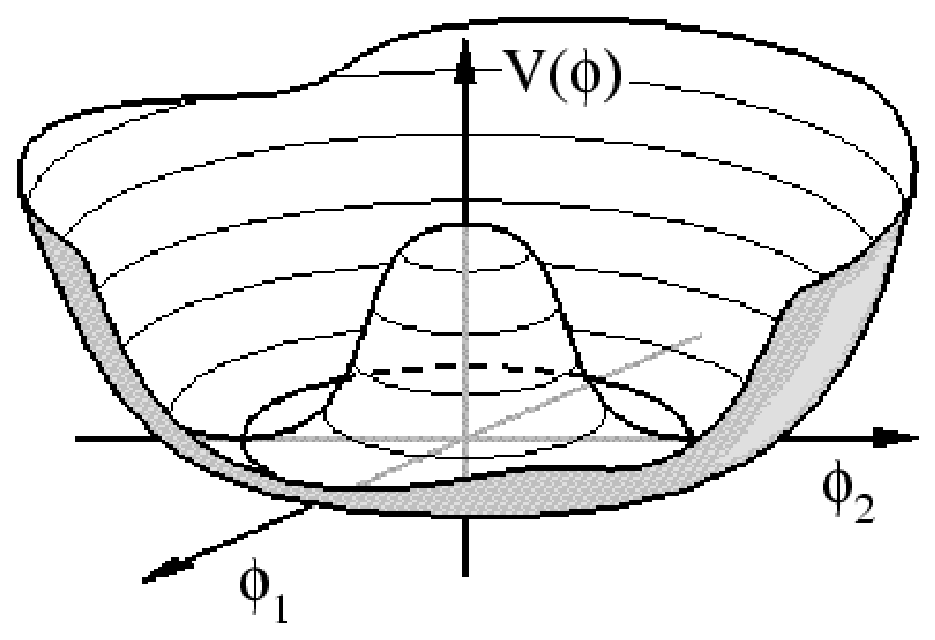
\includegraphics[width=0.50\textwidth]{eps/Theory/HiggsPotential.eps}
\end{center}
\vspace{-0.1in}
\caption{The Higgs "wine-bottle" potential~\cite{higgspotential}.}
\label{HiggsPotential}
\end{figure}

The strong interaction is an SU(3) gauge theory mediated by eight massless gauge bosons called gluons. The gluons interact with any particle that carries color charge, which in the Standard Model are quarks and the gluons themselves. The strong interaction exhibits an interesting property that the strength of the interaction decreases as the energy of the processes increases. Eq.~\ref{alphas}~shows the strong coupling parameter ($\alpha_{S}$) dependence on the energy of the process. 

\begin{equation}
\label{alphas}
\alpha_{S}(E) = \frac{12\pi}{33-2n_{f}\ln\left[\left(\frac{E}{\Lambda}\right)^{2}\right]}
\end{equation}

\noindent $n_{f}$ is the number of active\footnote{The number of active quark flavors depends on the energy of the process. At energies of $\sim100$ MeV, there are three quark flavors (u,d,s). At higher energies of $\sim10$ GeV, there are five quark flavors (u,d,s,c,b).} quark flavors and $\Lambda$ is the natural scale of the strong interaction ($\Lambda\sim$200 MeV).
The decreased coupling strength at energies greater than $\Lambda$ allows quarks to break their confined states and travel as bare color charges. As the quark begins to propagate however, it polarizes the vacuum between itself and its color partner until it becomes energetically favorable to create a new quark-antiquark pair. This process can repeat itself many times with a net effect of creating of a large number of strongly interacting particles traveling in the same direction as the originating colored particle. 

A summary of the guage bosons which mediate interactions in the Standard Model is given in Table~\ref{bosons}.

\begin{table}[!h!tbp]
\begin{center}
\caption{Properties of the fundamental spin-1 gauge bosons in the Standard Model~\cite{Yao:2006px}.}
\label{bosons}
\begin{tabular}{c|ccc}
%\multicolumn{4}{c}
%{\underline{Properties of the Fundamental Spin-1 Gauge Bosons}} \\
Interaction		&	Gauge Boson		&	Electric Charge		&	Mass [GeV] \\
\hline
Strong			&	Gluon (g)			&	0				&	0	\\
Weak			&	W				&	$\pm 1$e			&	80.4	\\
Weak			&	Z				&	0				&	91.2	\\
Electromagnetic	&	Photon ($\gamma$)	&	0				&	0	\\
\end{tabular}
\vspace{-0.1 in}
\end{center}
\end{table}
\subsection{Cabibbo-Kobayashi-Maskawa Quark Mixing Matrix}

It has been observed that the quantum states that describe a quark when produced via the strong interaction (e.g. $g\rightarrow b\bar{b}$) are not the same as the states used to describe the quark under a flavor changing weak transition (e.g. $W\rightarrow t\bar{b}$). The relationship between the strong and weak basis states is summarized by the Cabbibo-Kobayahski-Maskawa (CKM) unitary quark mixing matrix, shown in Eq.~\ref{ckm}.

\begin{equation}
\left[ \begin{array}{c}
d^{'}	\\
s^{'}	\\
b^{'}	\\
\end{array}\right]
=
\left[ \begin{array}{ccc}
V_{ud} & V_{us} & V_{ub} \\
V_{cd} & V_{cs} & V_{cb} \\
V_{td} & V_{ts} & V_{tb} \\
\end{array}\right]
\left[ \begin{array}{c}
d	\\
s	\\
b	\\
\end{array}\right]
\label{ckm}
\end{equation}

\noindent where $[d^{'}~s^{'}~b^{'}]^{T}$ are the weak eigenstates and $[d~s~b]^{T}$ are the strong eigenstates.

The CKM matrix contains the probabilities for charged current transitions of one quark to another within the same generation or between generations. For example, $V_{ud}$ is the probability for a down quark to transition to an up quark in a flavor changing weak decay. The experimentally determined values for the CKM matrix elements are shown in Eq.~\ref{ckmval}~\cite{Yao:2006px}. As seen from this matrix transitions within the same generation are preferred over transitions between generations.

\begin{equation}
\left[ \begin{array}{ccc}
0.97383^{+0.00024}	_{-0.00023}	&	0.2272^{+0.0010}_{-0.0010}			&	3.96^{+0.09}_{-0.09} \times 10^{-3}		\\
0.2271^{+0.0010}_{-0.0010}		&	0.97296^{+0.00024}_{-0.00024}		&	42.21^{+0.10}_{-0.80} \times 10^{-3}		\\
8.14^{+0.32}_{-0.64} \times 10^{-3}	&	41.61^{+0.12}_{-0.78} \times 10^{-3}		&	0.999100^{+0.000034}_{-0.000004}		\\
\end{array}\right]
\label{ckmval}
\end{equation}

Of particular interest for this thesis is the $V_{tb}$ matrix element. This matrix element has never been directly measured although it is heavily constrained once the unitarity of the matrix is imposed. A direct measurement of this quantity is possible through an observation of electroweak top quark production. The measurement of this process in $\ppbar$~collisions at the Tevatron is the subject of this thesis.

\section{The Top Quark}
\label{topquark}

In the Standard Model all quarks exist in left-handed isospin doublets. Thus when the bottom quark was discovered in 1977, a new left-handed isospin partner quark was required to exist. The long predicted top quark was finally discovered in $p\bar{p}$ collisions at the Tevatron in 1995 by the $\dzero$ and CDF collaborations~\cite{Abe:1995hr,Abachi:1995iq}. The top quark is unique from previously measured quarks because its mass is nearly forty times larger than the next heaviest quark with a mass of $171.4~\pm~2.1$~GeV/$c^{2}$~\cite{Brubaker:2006xn}.

Due to its very large mass the top quark has an relatively large decay width. The width of the top quark can be calculated within the framework of the Standard Model and is shown in Eq.~\ref{toplife}\footnote{In Eq.~\ref{toplife}, $G_{F}$ is the Fermi constant, $m_{t}$ is the top quark mass, $m_{W}$ is the $W$ boson mass, and $\alpha_{S}$ is the strong coupling constant.}. The top quark width is estimated to be $1.53$~GeV, which can be converted to a lifetime of $0.4 \times 10^{-24}$~sec. This lifetime is almost one order of magnitude smaller than the typical time scale for all strong interactions ($1/\Lambda\sim10^{-23}$~s) and leads to the property that the top quark does not form strong bound states~\cite{Bigi:1986jk}.

\begin{equation}
\Gamma(t \rightarrow Wb) = \frac{G_{F}m_{t}^{3}|V_{tb}|^{2}}{8\pi\sqrt{2}} \left[1-\frac{m_{W}^{2}}{m_{t}^{2}}\right]\left[1+2\frac{m_{W}^{2}}{m_{t}^{2}}\right]\left[1-\frac{2\alpha_{s}(4\pi-15)}{18\pi}\right]
\label{toplife}
\end{equation}

%Another interesting property of the top quark is it's relatively large coupling to the predicted Higgs boson. Within the Standard Model all particles acquire mass through the Higgs mechanism. The mass of the particle is related to the coupling strength of the particle to the Higgs field. The top quark's large mass requires that it has a coupling to the Higgs field of order 1. The order unity coupling of the top quark to the Higgs field suggests that it may have a unique role in electroweak symmetry breaking~\cite{PhysRevD.41.1647}.

At the Tevatron the top quark is primarily produced through pair production via the strong interaction. The cross section for this process has been calculated as $6.77 \pm 0.42$~pb for a top mass at $175$~GeV~\cite{Kidonakis:2003qe}. The $t\bar{t}$ system has been extensively studied at the Tevatron and the measured cross section in all decay channels agrees well with theory~\cite{Abazov:2006ka,Abazov:2005yt,Abazov:2005ey,Abazov:2005ex,Abulencia:2006se,Abulencia:2006kv,Abulencia:2006in,Abulencia:2006yk,Acosta:2005zd,Acosta:2005am}. The leading order Feynman diagrams for $\ttbar$~production are shown in Fig.~\ref{ttbar}.

\begin{figure}[!h!tbp]
\begin{center}
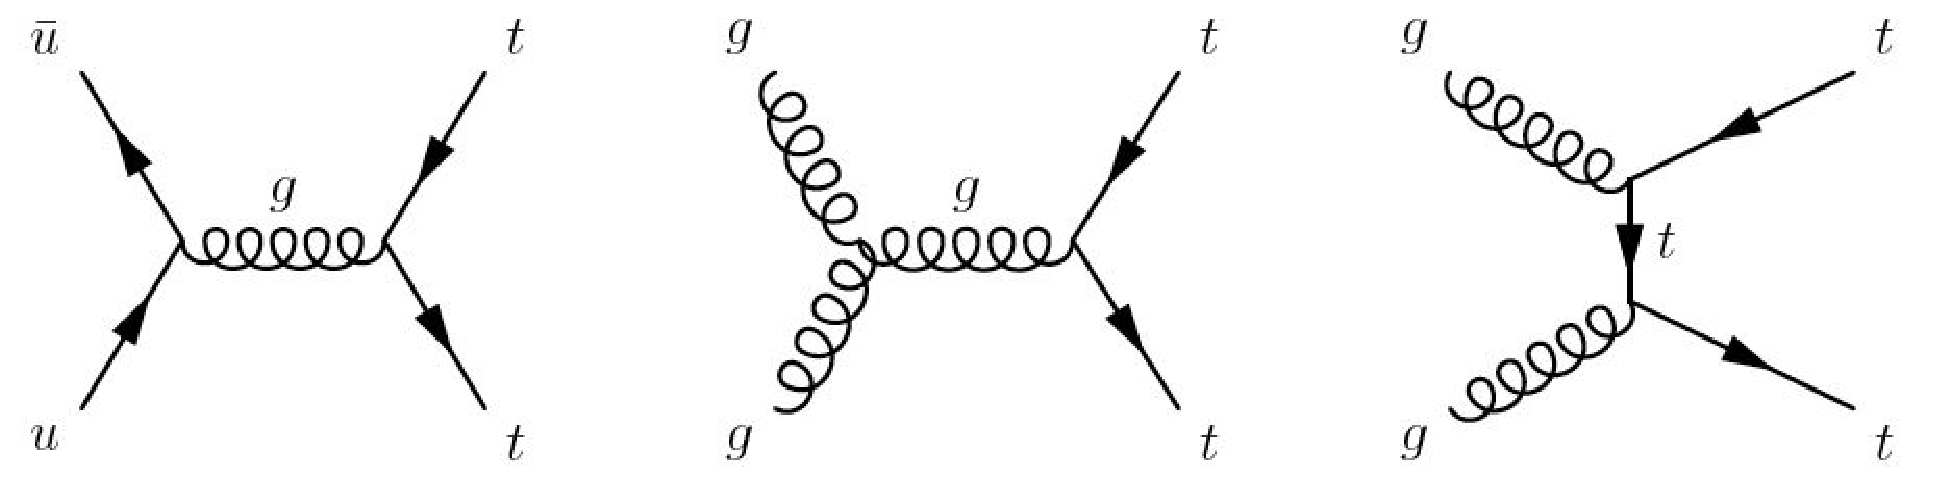
\includegraphics[width=0.9\textwidth]{eps/Theory/TTbar.eps}
\end{center}
\vspace{-0.1in}
\caption{Main leading order $t\bar{t}$ pair production Feynman diagrams~\cite{Jabeen:2006km}.}
\label{ttbar}
\end{figure}

\section{Electroweak Top Quark Production}
\label{electroweaktopquark}

Top quarks can also be produced via an electroweak interaction commonly called single top because only one top quark is produced in the event. At the Tevatron there are two dominant modes of single top production. The first is the $s$-channel process defined by a virtual time-like ($Q^{2}_{W} > 0$) $W$ boson formed from a $q\bar{q}'$ annihilation and decaying to a top and bottom quark. The second is the $t$-channel process defined by a virtual space-like ($Q^{2}_{W} < 0$) $W$ boson produced by a light and bottom quark exchange and producing a forward scattered light quark and a top quark. There is a third mode of production where the top quark is created in association with an on-shell ($Q^{2}_{W}=M^{2}_{W}$) $W$ boson; however, the cross section for this production mode is negligible at the Tevatron. Feynman diagrams for the $s$-channel and $t$-channel production modes are shown in Figs.~\ref{schannel} and~\ref{tchannel}.  The $s$-channel and $t$-channel cross sections have been calculated in~\cite{Smith:1996ij,PhysRevD.56.3114,Stelzer:1997ns,Harris:2002md,Sullivan:2004ie,Cao:2004ap,Cao:2005pq,Kidonakis:2006bu} with the cross sections used in the data analysis shown in Table~\ref{singletopcross}.

\begin{figure}[!h!tbp]
\begin{center}
\includegraphics[width=0.45\textwidth]{eps/Theory/schannel.eps}
\end{center}
\vspace{-0.1in}
\caption{The leading order Feynman diagram for the $s$-channel single top production mode~\cite{Jabeen:2006km}.}
\label{schannel}
\end{figure}

\begin{figure}[!h!tbp]
\begin{center}
\includegraphics[width=0.50\textwidth]{eps/Theory/tchannel.eps}
\end{center}
\vspace{-0.1in}
\caption{The leading order (left) and an important next-to-leading order (right) Feynman diagrams for the $t$-channel single top production mode~\cite{Jabeen:2006km}.}
\label{tchannel}
\end{figure}

As stated earlier in this chapter, the top quark prefers to decay to a $W$ boson and a $b$~quark. The common decay mode to detect single top events is when the $W$ boson either decays to an electron or muon and an associated neutrino\footnote{The $W\rightarrow \tau \nu_{\tau}$ and $W\rightarrow q\bar{q}^{'}$ channels are not considered in this thesis due to the large expected background rate.}. For the $s$-channel, the final state particles for the leading order process are (1) lepton, (1) neutrino, and (2) $b$ quarks. The $t$-channel final state is characterized by (1) lepton, (1) neutrino, (1) light quark, and at least one (1) $b$ quark. The $s$-channel and $t$-channel processes are sometimes referred to as $tb$ and $tqb$, respectively.

\vspace{0.2in}
\begin{table}[!h!tbp]
\begin{center}
\caption{Total cross sections for single top quark
production at $\sqrt{s} = 1.96$~TeV with $m_t=175$~GeV.}
\label{singletopcross}
\begin{minipage}{2.2 in}
\begin{tabular}{lc}
Process & Cross Section [pb] \\
\hline
$s$-channel ($tb$)	&	$0.88 \pm 0.11$		\\
$t$-channel ($tqb$)	&	$1.98 \pm 0.25$		\\
$s+t$			&	$2.86 \pm 0.27$		\\
\end{tabular}
\vspace{-0.1 in}
\end{minipage}
\end{center}
\end{table}



\subsection{Motivation for Single Top}
\label{motivation}

Measuring the single top quark production cross section ($\sigma$) and the angular differential cross section ($\frac{d\sigma}{d\Omega}$) is interesting as a test of the Standard Model as well as a probe for new physics beyond the Standard Model. Perhaps the most interesting product of a single top quark cross section measurement is a direct determination of the CKM matrix element $|V_{tb}|$ since the cross section is proportional to the square of this quantity ($\sigma\propto|V_{tb}|^{2}$).
If one assumes a unitary 3x3 CKM matrix then by measuring $|V_{ub}|$ and $|V_{cb}|$, $|V_{tb}|$ is required to be within the following range:
\begin{equation}
0.9991 < |V_{tb}| < 0.9994
\label{vtb}
\end{equation}

By relaxing the assumption on a unitary 3x3 CKM matrix~\cite{PhysRevD.63.014018}, $|V_{tb}|$ is allowed in the following range:
\begin{equation}
0.06 < |V_{tb}| < 0.9994
\end{equation}

A measurement of $|V_{tb}|$ that differed significantly from the range shown in Eq.~\ref{vtb} would be clear evidence for physics beyond the Standard Model such as a fourth generation of quarks.

Another interesting test of the Standard Model that can be made as a result of measuring single top is to probe the structure of the $Wtb$ vertex. In the Standard Model all single top quarks are produced via the left-handed electroweak interaction. If one were to boost into the top quark rest frame and know the four momenta of the decay products, then the angular decay distribution for the charged lepton from the $W$ boson decay would follow the distribution shown in Eq.~\ref{decay} where the angle $\theta_{l}$ is calculated with respect the top quark spin vector.

\begin{equation}
\frac{1}{\sigma}\frac{d\sigma}{d(\cos(\theta_{l})} = \frac{1}{2}\left[ 1 + \cos(\theta_{l}) \right]
\label{decay}
\end{equation}

In practice, boosting into the correct top quark frame does not always result in 100$\%$ left handed polarized ($\hat{s} \bullet \hat{p}=-1$) top quarks~\cite{Mahlon:1998uv}. For the $s$-channel process there an ambiguity resulting from the possibility of the up-type quark originating from the proton and the down-type quark origination from anti-proton and the reverse case. By boosting into the top quark frame and choosing the spin of the top quark along the direction of the anti-proton, one can expect to measure 98$\%$ polarization of top quarks. For the $t$-channel, the addition of higher order diagrams reduces the fraction of polarized top quarks. By boosting into the top frame and choosing the spin of the top quark along the direction of the forward down-type quark as seen in Fig.~\ref{tchannel}, one expects to measure 96$\%$ of top quarks to be polarized. By measuring the degree to which top quarks are polarized one can test the left-handed structure of the $Wtb$ vertex.

Finally, the $s$ and $t$-channel cross sections are sensitive to new particles predicted by theories beyond the Standard Model~\cite{PhysRevD.63.014018}. The Standard Model $s$-channel amplitude will interfere with any other diagram that includes a charged vector boson as the interaction mediator. One example of such a boson is the $W^{'}$ which results from an additional SU(2) group structure in the electroweak Lagrangian. The leading order Feynman diagrams for the $W^{'}$ boson production is shown in Fig.~\ref{schannelnew}.

\begin{figure}[!h!tbp]
\begin{center}
\includegraphics[width=0.45\textwidth]{eps/Theory/wprime.eps}
\end{center}
\vspace{-0.1in}
\caption{The leading order Feynman diagrams for the $s$-channel like process involving a $W^{'}$ boson~\cite{Jabeen:2006km}.}
\label{schannelnew}
\end{figure}

The Standard Model $t$-channel diagram will interfere primarily with new diagrams that involve flavor changing neutral currents (FCNC) including the top quark, which are predicted by models such as supersymmetry and technicolor~\cite{PhysRevD.63.014018}. A leading order Feynman diagram for this process is shown in Fig.~\ref{tchannelnew}.

\begin{figure}[!h!tbp]
\begin{center}
\includegraphics[width=0.2\textwidth]{eps/Theory/FCNC.eps}
\end{center}
\vspace{-0.1in}
\caption{A leading order Feynman diagram for a $t$-channel-like process produced through FCNC~\cite{Jabeen:2006km}.}
\label{tchannelnew}
\end{figure}

Thus, by measuring each production cross section to high accuracy, one can test the validity of new physics models.



\subsection{Signal Event Generation}
\label{singletopgeneration}

An important part of a physics analysis is to have a determination of the kinematic distributions of signal events along with a cross section estimate to provide a normalization for the number of events to expect from the $\ppbar$~collisions. Both of these tasks can be accomplished by Monte Carlo generators. Monte Carlo generators use a set of random numbers to sample the N-dimensional phase space defined by the number of initial and final state particles in the event. The trial event is given a weight determined by the differential cross section, shown in Eq.~\ref{diffcross}, and is selected as a signal event if the weight is greater than a new random number sampled from the properly normalized differential cross section distribution. This method allows for more events to be selected from a region in phase space where the differential cross section is large and few events are selected from regions of low differential cross section. The final step of the Monte Carlo simulation is to hadronize\footnote{Hadronization is the process of forming bound states (hadrons) between two or three quarks. A bound state of two quarks is called a meson and a three quark bound state is called a baryon.} and shower\footnote{A shower, or parton shower, is the result of multiple gluon emission from final state particles.} the final state partons and allow for additional energy in the event resulting from the breakup of the two protons in the collision. This final step is performed using the Pythia~\cite{Sjostrand:2001yu} Monte Carlo generator.

\begin{equation}
\label{diffcross}
\pderiv{\sigma(\vec{y})}{\vec{y}} = \sum_{i,j} f_{i}(Q^{2},x_{1})f_{j}(Q^{2},x_{2}) \times \pderiv{\sigma_{hs,ij}(\vec{y})}{\vec{y}}
\end{equation}

In Eq.~\ref{diffcross}, $\pderiv{\sigma_{hs,ij}(\vec{y})}{\vec{y}}$ is the differential cross section for the parton-parton\footnote{A parton is a constituent particle within the proton.} collision and $f_{i}(x_{1},Q^{2})$ and $f_{j}(x_{2},Q^{2})$ are the parton distribution functions (PDFs) that describe the number density of partons $i$ and $j$ inside the proton. The two parameters in these functions are the proton momentum fraction ($x=p_{\rm{parton}}/p_{\rm{proton}}$) and the energy scale (factorization scale) at which the two partons collide (Q). A plot of the parton density functions from the CTEQ~\cite{Pumplin:2002vw} collaboration is shown in Fig.~\ref{cteqpdfs} for two distinct momentum transfers. 

\begin{figure}[!h!tbp]
\begin{center}
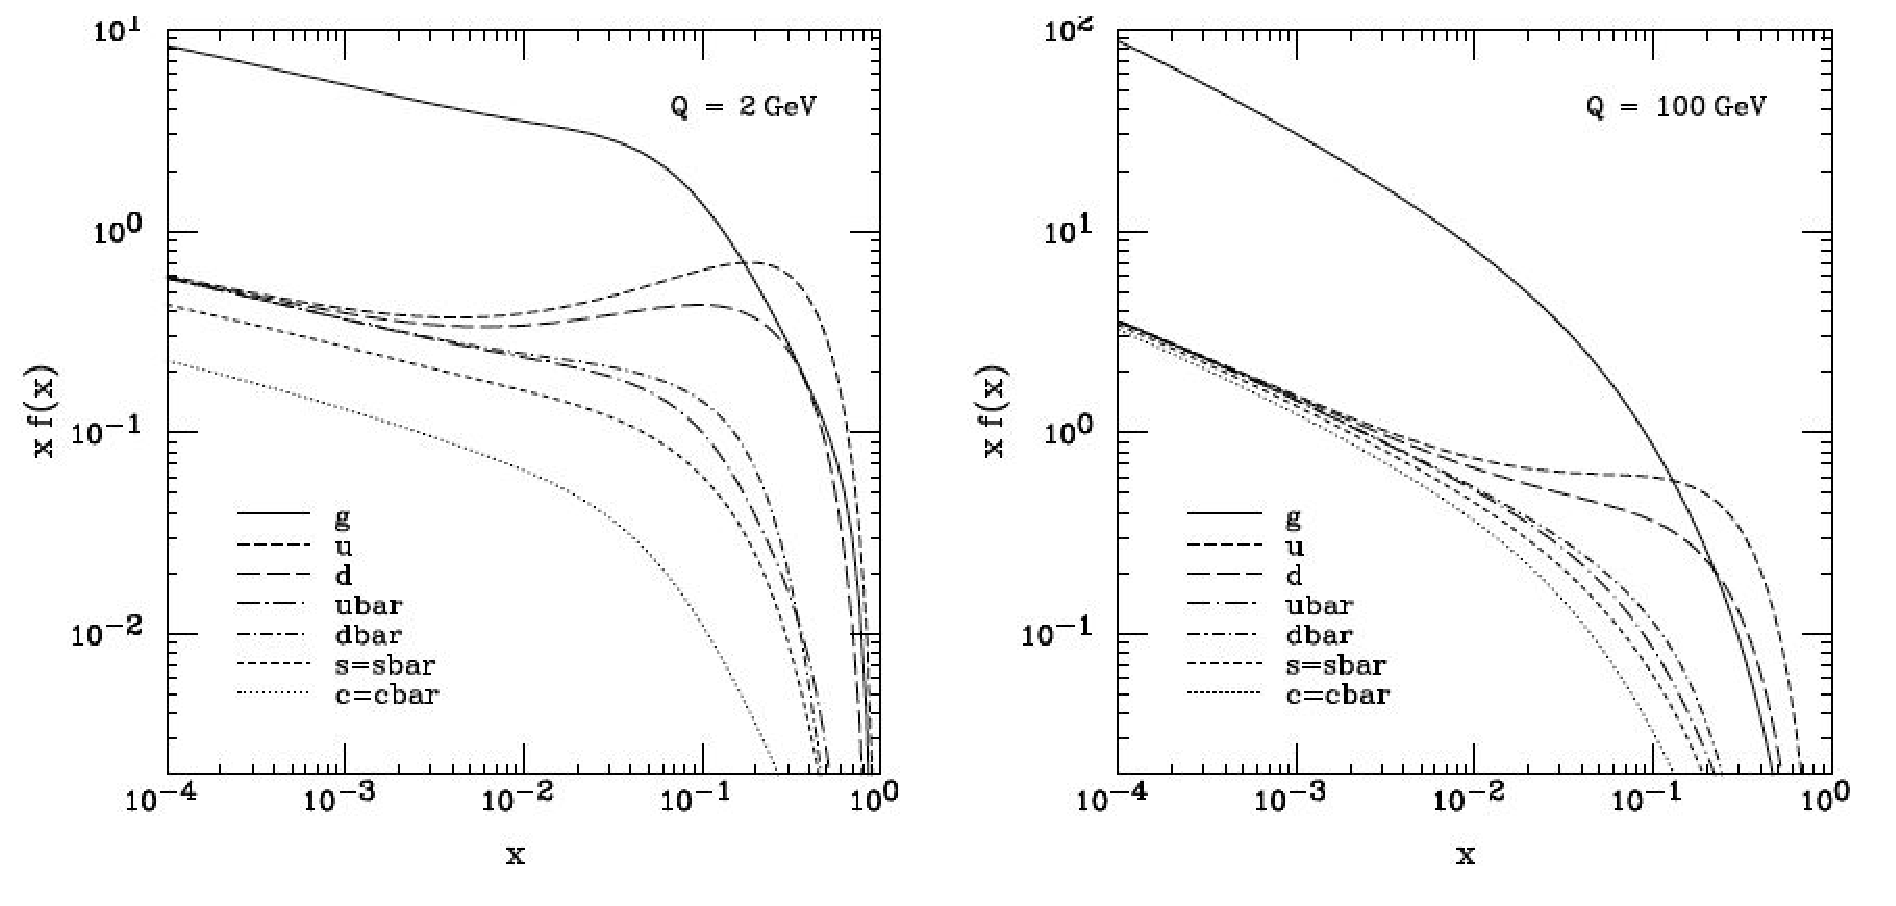
\includegraphics[width=0.90\textwidth]{eps/Theory/CTEQ_pdfs.eps}
\end{center}
\vspace{-0.1in}
\caption{CTEQ 6M parton distribution functions for the gluon and all quark flavors for a small momentum transfer (left) and large momentum transfer (right). The $x$-axis is the proton momentum fraction of the parton and the $y$-axis is the parton density~\cite{Pumplin:2002vw}.}
\label{cteqpdfs}
\end{figure}


Single top signal events are generated using the CompHEP based SingleTop~\cite{Boos:SingleTop} Monte Carlo generator. The following two sections describe the generation of $s$-channel and $t$-channel production. All events were generated using CTEQ6L1 PDFs. The $s$-channel events were generated with $Q^{2}=m_{t}^{2}$ and $t$-channel events were generated with $Q^{2}=(m_{t}/2)^{2}$.

\subsubsection{$s$-channel Generation Using CompHEP}
\label{schannelgen}

It has been shown in~\cite{Sullivan:2004ie} that $s$-channel kinematic distributions between leading order (LO) and next-to-leading order (NLO) in $\alpha_{s}$ are the same up to an overall normalization. The ratio of NLO to LO events, called a k-factor, is $1.3$~for the $s$-channel production mode. Fig.~\ref{schannelevents} shows the transverse momentum ($p_{T}$) and pseudorapidity\footnote{The pseudorapidity is related to the polar angle $\theta$. More discussion of this variable is given in Chaper~\ref{experiment}.}($\eta$) distributions for $s$-channel events generated by SingleTop.


\begin{figure}[!h!tbp]
\begin{center}
\includegraphics[width=0.49\textwidth]{eps/Theory/Hist_tb_Pt.eps}
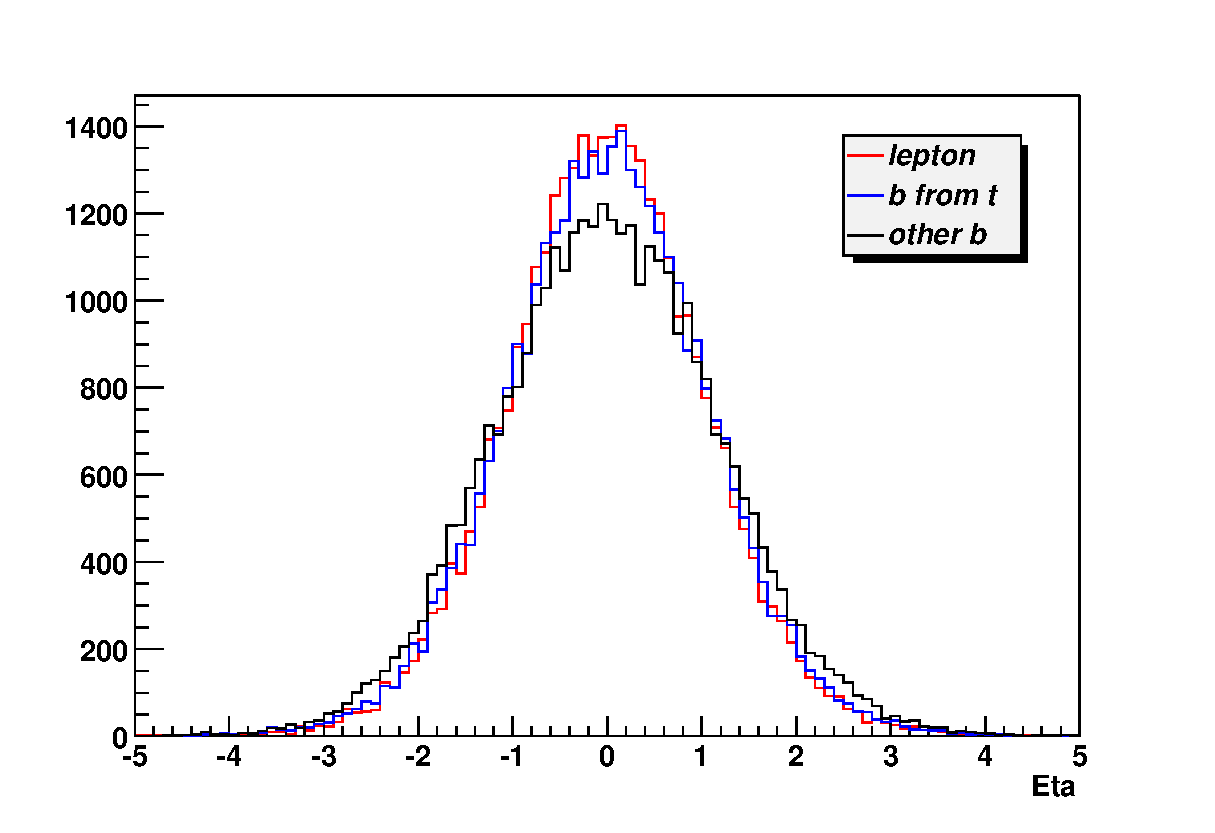
\includegraphics[width=0.49\textwidth]{eps/Theory/Hist_tb_Eta.eps}
\end{center}
\vspace{-0.1in}
\caption{$p_{T}$ (left) and $\eta$ (right) distributions of final state particles in $s$-channel events~\cite{Jabeen:2006km}.}
\label{schannelevents}
\end{figure}


\subsubsection{$t$-channel Generation Using CompHEP and Pythia}
\label{tchannelgen}

Generating $t$-channel Monte Carlo events is slightly more difficult than $s$-channel events because the effective cross section of higher order Feynman diagrams ($qg\rightarrow q^{'}tb$), shown in Fig.~\ref{tchannel}, is of the same order as the leading order diagram ($qb\rightarrow tq^{'}$). A proper treatment of the combination is required to avoid double counting regions of phase space where the two matrix elements overlap. The SingleTop generator avoids double counting by defining two distinct regions of phase space where the different processes are the dominant contribution to the total $t$-channel cross section. The first region of phase space is defined by $p_{T}(b)<10$~GeV. In this region the final state $b$~quark is produced by Pythia through initial state radiation (ISR). The second phase space region is defined by $p_{T}(b)>10$~GeV. In this region the $b$~quark is produced by the next-to-leading order Feynman diagram shown in Fig~\ref{tchannel}. To ensure a smooth transition from low to high $b$~quark $p_{T}$, the weight for the low $p_{T}$ region is multiplied by a k-factor to make the leading order Pythia generated $b$~quark $p_{T}$~match the next-to-leading order $b$~quark $p_{T}$ distribution. The k-factor used at the Tevatron is 1.21 and the effective NLO cross section used in the SingleTop generator is shown in Eq.~\ref{tchannelcross}.

\begin{equation}
\label{tchannelcross}
\sigma_{\rm{NLO}} = K\sigma_{\rm{Pythia}}|_{P_{T}(b)<10} + \sigma_{\rm{CompHEP-SingleTop}}|_{P_{T}(b)>10}
\end{equation}

The result of the $b$~quark $p_{T}$ splicing is an almost exact reproduction of many NLO differential distributions. Fig.~\ref{tchannelevents} shows $p_{T}$ and $\eta$ distributions for $t$-channel events generated by SingleTop.

\begin{figure}[!h!tbp]
\begin{center}
\includegraphics[width=0.49\textwidth]{eps/Theory/Hist_tqb_Pt.eps}
\includegraphics[width=0.49\textwidth]{eps/Theory/Hist_tqb_Eta.eps}
\end{center}
\vspace{-0.1in}
\caption{$p_{T}$ (left) and $\eta$ (right) distributions of final state particles in $s$-channel events~\cite{Jabeen:2006km}.}
\label{tchannelevents}
\end{figure}


 

% ========== Chapter 3

\chapter{Experimental Apparatus}
\label{experiment}

All data used in the single top quark analysis was produced by high energy $\ppbar$ collisions at the Tevatron accelerator and recorded by the $\dzero$~detector. The Tevatron is currently the only collider with enough center of mass energy to directly produce top quarks in relative abundance. Section~\ref{tevatron} describes how protons are accelerated to an energy of 980 GeV as well as how antiprotons are created to produce $\ppbar$~collisions at $\sqrt{s}=1.96$~TeV. Sections~\ref{ppbarcollisions} and~\ref{coordinate} give an introduction to $\ppbar$~collisions at the Tevatron and explain several useful quantities which described particles produced in the collisions. Finally, Section~\ref{detector} describes the $\dzero$~detector that is used to collection information about the particles produced in the $\ppbar$~collisions. 

\section{Fermilab Accelerator Complex}
\label{tevatron}

The Fermilab accelerator complex is a chain of accelerators designed to produce and collide two circulating beams of protons and antiprotons each with an energy of 980 GeV. Fermilab employs five unique accelerators to create and accelerate protons and antiprotons: the Cockcroft-Walton, the LINAC, the Booster, the Main Injector, and the Tevatron. Fig.~\ref{FermilabAccelerator} shows a schematic of these accelerators.

\begin{figure}\centering
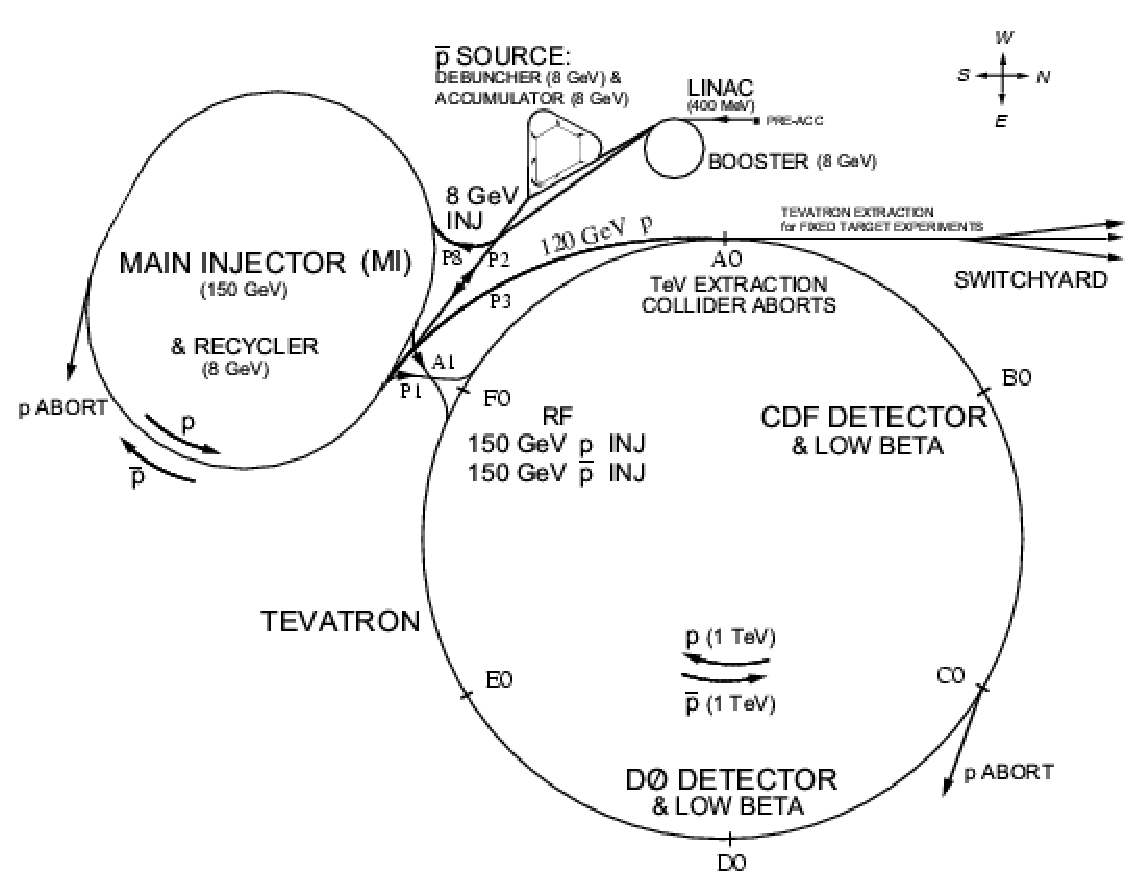
\includegraphics[width=6in,angle=0]{eps/Tevatron/Tevatron.eps}
\caption{Schematic of the Fermilab accelerator complex~\cite{Haas:2004rx}.}
\label{FermilabAccelerator}
\end{figure}

\subsection{Cockcroft-Walton}
The first accelerator in the chain is the Crockroft-Walton. In this accelerator a hydrogen gas is heated which allows an additional electron to bond with the hydrogen atom producing a net negative charge. The Crockroft-Walton is a DC voltage ladder that produces a voltage difference of 750~kV across which the newly negatively hydrogen ions are accelerated.

\subsection{LINAC}
After the negatively charged hydrogen ions have been accelerated to an energy of 750keV, they are further accelerated by the LINAC (LINear ACcelerator). The LINAC is a 130-m long set of metallic drift tubes separated by vacuum gaps. An alternating electric field produced by a radio frequency (RF) power source accelerates the negatively charged hydrogen ions across the gap while the electric field is parallel with the ion direction of motion. When the field direction reverses the ions are shielded by the metallic drift tubes. As the ions increase their speed the gap length and drift tube length increases as shown in Fig.~\ref{LINAC}. Because the LINAC uses an alternating electric field the continuous ion beam produced by the Crockoft-Walton is altered such that the protons are concentrated or ``bunched" together. By the end of the acceleration the proton bunches are separated by 5 ns and have an energy of 400 MeV. Finally, the orbital electrons are removed by passing the ions through a carbon foil leaving behind the positively charged protons.

\begin{figure}[!h!tbp]
\begin{center}
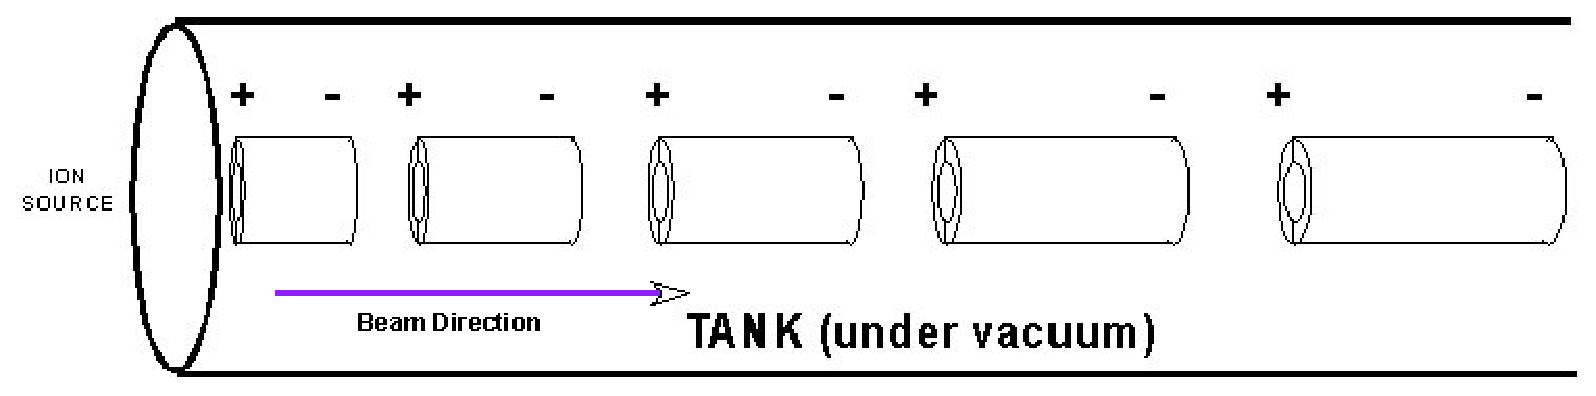
\includegraphics[width=0.75\textwidth]{eps/Tevatron/LINAC.eps}
\end{center}
\vspace{-0.1in}
\caption{Cartoon example of the linear accelerator's alternating series of gaps and drift tubes~\cite{proton}.}
\label{LINAC}
\end{figure}

\subsection{Booster}
The next accelerator in the chain is the Booster, which is a circular synchrotron accelerator 475-m in circumference. The Booster consists of RF cavities that accelerate the 400 MeV proton bunches to an energy of 8 GeV. The proton bunches circulate the Booster 16,000 times and the entire acceleration process takes 33 ms.

\subsection{Main Injector}
The Main Injector is the next accelerator in the chain after the Booster. This accelerator uses RF cavities to accelerate the proton bunches to an energy of 120 GeV and employs strong magnets to keep the protons moving along a circular path. After the acceleration there are two possible paths for the protons: $\bar{p}$~production or continued acceleration. The protons that will eventually circulate in the Tevatron ring are further accelerated to an energy of 150 GeV and then continue to circulate the Main Injector ring until needed~\cite{proton}. The remaining protons are used to create antiprotons that will also eventually circulate in the Tevatron ring. Antiprotons are created when 120 GeV protons from the Main Injector strike a fixed 7 cm thick nickel target producing a spray of short lived particles and anti-particles. From this spray roughly 20 antiprotons are produced for every million protons used~\cite{Antiproton}. All particles produced from the collision are focused and collimated by a lithium lens. A bending magnetic is employed to separate the negatively charged antiprotons from all positively charged particles. To remove the remnant bunch structure the antiprotons are passed through a debuncher, which separates the antiprotons in space-time as well as reducing their energy spread. A process known as stochastic cooling is applied to further reduce the energy spread. This process uses ultra-cold electronics (-$269^{\circ}$~C) to detect and alter the particles trajectories to make their orbits and thereby their energies more uniform. Because each $\ppbar$~collision requires $\sim10^{10}$ antiprotons the final stage for $\bar{p}$~production is to collect and store large quantities of antiprotons. This is done with the accumulator, which allows for many circulating beams of antiprotons to be kept for many hours. Once enough antiprotons have been collected they are sent to the Main Injector where they are accelerated to a final energy of 150 GeV.

\subsection{Tevatron}

The Tevatron is the final acceleration stage for the protons and antiprotons, which reach an energy of 980 GeV using RF cavities in the same manner as the Booster and the Main Injector~\cite{tevatron}. The Tevatron uses nearly 1,000 superconducting magnets running at $4.3^{\circ}$~K with a magnetic field strength of $4.2$~T to bend the two circulating beams around the nearly 6~$\frac{1}{2}$ km circumference ring. At an energy of 980 GeV the bunches circulate the Tevatron ring nearly 57,000 times per second crossing one-another every 396 ns. The two circulating beams are separated in the ring to avoid direct collisions unless they are further focused. In the Tevatron ring there are two places where the beams are focused, which correspond to the two large experiments: $\dzero$ and CDF.

\section{$\ppbar$~Collisions}
\label{ppbarcollisions}

When the two circulating beams at the Tevatron are brought into focus, an enormous range of kinematically allowed processes and final state decays are possible. While the outcome of a particular $\ppbar$~collision is random, the rate at which certain processes occur can be calculated within the Standard Model framework. The most common type of collision is an inelastic $\ppbar$~collision which produces one or more particles scattered at low angles with respect to the beam axis. These processes usually do not involve much energy transfer between the colliding particles and are therefore called low-$p_{T}$ events. More rare processes, such as top quark or $W$ boson production, require much more energy to be transferred between colliding particles. These processes occur when one of the constituent quarks or gluons inside the proton collide with another quark or gluon from the antiproton. This process is referred to as the hard scatter process. The hard scatter process can produce on-shell resonances ($Q^{2} = M^{2}$) of heavy particles such as a $W$ Boson or sometimes it can produce very short lived vritual particles ($Q^{2} \neq M^{2}$) such as the case with $s$-channel single top quark production where a $W$ boson is produced with $Q^{2} > M_{W}^{2}$.

The heavy particles produced in the hard scatter collision will decay into more stable particles as governed by the interactions allowed in the Standard Model. For very heavy particles with short lifetimes the decay occurs in a space much smaller than the resolution of any detector. For instance, the top quark lifetime is $\sim10^{-24}$~s which is more than nine orders of magnitude smaller than the fastest detector electronics. In fact almost all short-lived particles produced in the hard scatter can not be measured directly, but instead their presence is inferred from precise measurements of the their decay products.

The remainder of this chapter is dedicated to describing the $\dzero$~detector and how it makes the measurements required to infer the presence of heavy resonances such as the top quark. Section~\ref{coordinate} gives a short introduction to the coordinate system convention used throughout the rest of the chapter as well as introduces several new units typically used in high energy physics. Section~\ref{detector} describes the $\dzero$~detector and explains how it is used to measure the particles resulting from the $\ppbar$~collisions at the Tevatron.

\section{Coordinate System and Units Convention}
\label{coordinate}

The $\dzero$~detector is typically referenced using a spherical coordinate system ($r$,$\theta$,$\phi$) with an origin located at the center of the detector. The polar angle $\theta$ is defined with respect to the beam axis where $0^{\circ}$ is aligned with the proton direction and $180^{\circ}$ is aligned with the antiproton direction. The azimuthal angle $\phi$ is defined with respect to the $x$-axis as shown in Fig.~\ref{coordinate-eps}. The $z$-axis is defined to be parallel with the beam axis with the positive direction corresponding to $\theta = 0^{\circ}$ and the negative direction corresponding to $\theta = 180^{\circ}$.

\begin{figure}[!h!tbp]
\begin{center}
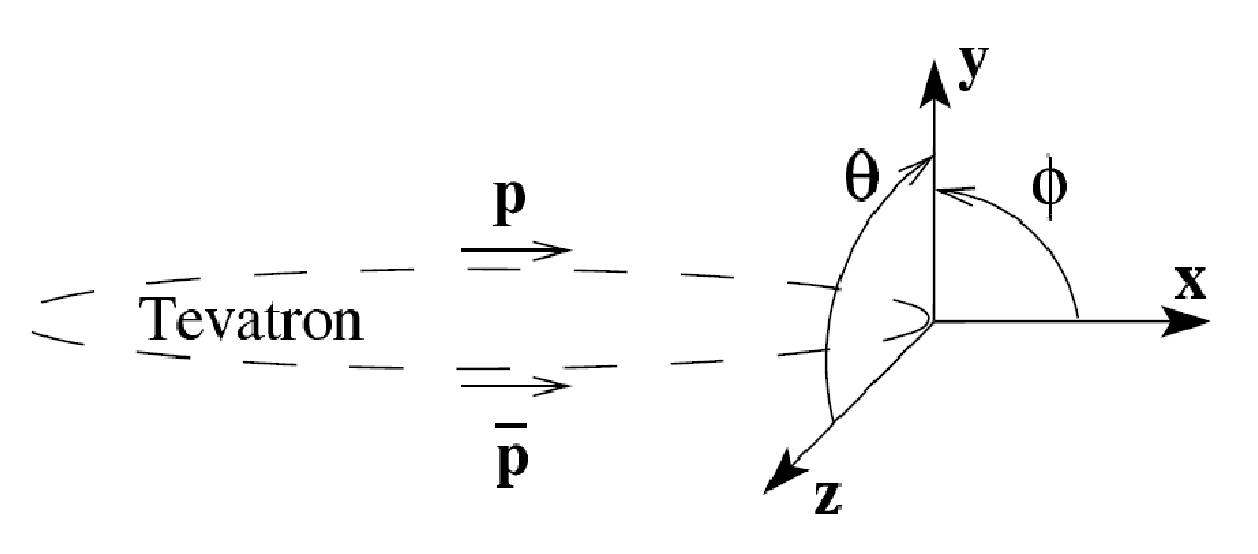
\includegraphics[width=0.75\textwidth]{eps/Tevatron/Coordinate.eps}
\end{center}
\vspace{-0.1in}
\caption{$\dzero$ coordinate system with respect to the Tevatron ring~\cite{Stelzer:2005kz}.}
\label{coordinate-eps}
\end{figure}

It often convenient to convert the angle $\theta$ to a quantity called pseudorapidity $\eta$ defined in Eq.~\ref{pseudorapidity}.

\begin{equation}
\label{pseudorapidity}
\eta = -\ln \left[ \tan \left( \frac{\theta}{2} \right) \right]
\end{equation}

This quantity is identical, in the limit of massless particles, to the true rapidity $y$, shown in Eq.~\ref{rapidity}, which is invariant under a Lorentz boost along the $z$-direction. This is useful because $\ppbar$~collisions at the Tevatron usually occur with such a boost. The pseudorapidity is $0$ for a particle with $\theta = 90^{\circ}$ and approaches $\infty$ as $\theta \rightarrow 0^{\circ}$.

\begin{equation}
\label{rapidity}
y = \frac{1}{2}\log \left[ \frac{E + p_{z}}{E - p_{z}} \right]
\end{equation}

Another quantity used when describing the relationship between two objects or the size of an object in the $\dzero$~detector is the solid angle $\Delta R$ defined in terms of $\Delta\phi=\phi_{1} - \phi_{2}$~and $\Delta\eta=\eta_{1} - \eta_{2}$.

\begin{equation}
\Delta R = \sqrt{(\Delta\phi)^{2} + (\Delta\eta)^{2}}
\end{equation}

Finally, the luminosity is important when describing the intensity of an interaction or of the accumulated amount of data. The rate of a certain process is equal to the luminosity $\mathcal{L}$ times the Lorentz invariant cross section $\sigma$, as shown in Eq.~\ref{rate}.

\begin{equation}
\label{rate}
\rm{Rate} = \frac{dN}{dt} = \sigma * \mathcal{L}
\end{equation}

Most cross sections at the Tevatron are given in terms of pico-barns ($10^{-36}$~cm$^{2}$) thus the units of luminosity are pb$^{-1}$s$^{-1}$. The time integrated luminosity $\int \mathcal{L} dt$, with units of pb$^{-1}$, is used when discussing the total number of collected events.

\section{\dzero~ Detector}
\label{detector}

The $\dzero$~detector~\cite{Abazov:2005pn} is a collection of smaller sub-detectors working in tandem  to detect and measure all particles produced from the hard scatter collision. The inner-most detectors near the beam pipe are the tracking detectors, described in Section~\ref{tracking}, which record the paths of charged particles as they enter and leave the detector. The next layer of the detector is the calorimeter, described in Section~\ref{calorimetry}. The calorimeter measures the energy of the lightest electromagnetically interacting particles, such as the electron and the photon, and strongly interacting particles, such as pions or neutrons. Another sub-detector, called the luminosity monitor, described in Section~\ref{luminositydetector}, is designed to record the presence of an inelastic $\ppbar$~collision in the bunch crossing. This information is used in the analysis to normalize backgrounds and expected signal yields. The outer-most layer of the $\dzero$~detector is the muon detector, which is described in Section~\ref{muondetector}. Once the collision has been measured a complex set of trigger decisions, described in Section~\ref{triggersystem}, must be satisfied before the event is recorded to tape for later analysis.

\begin{figure}[!h!tbp]
\begin{center}
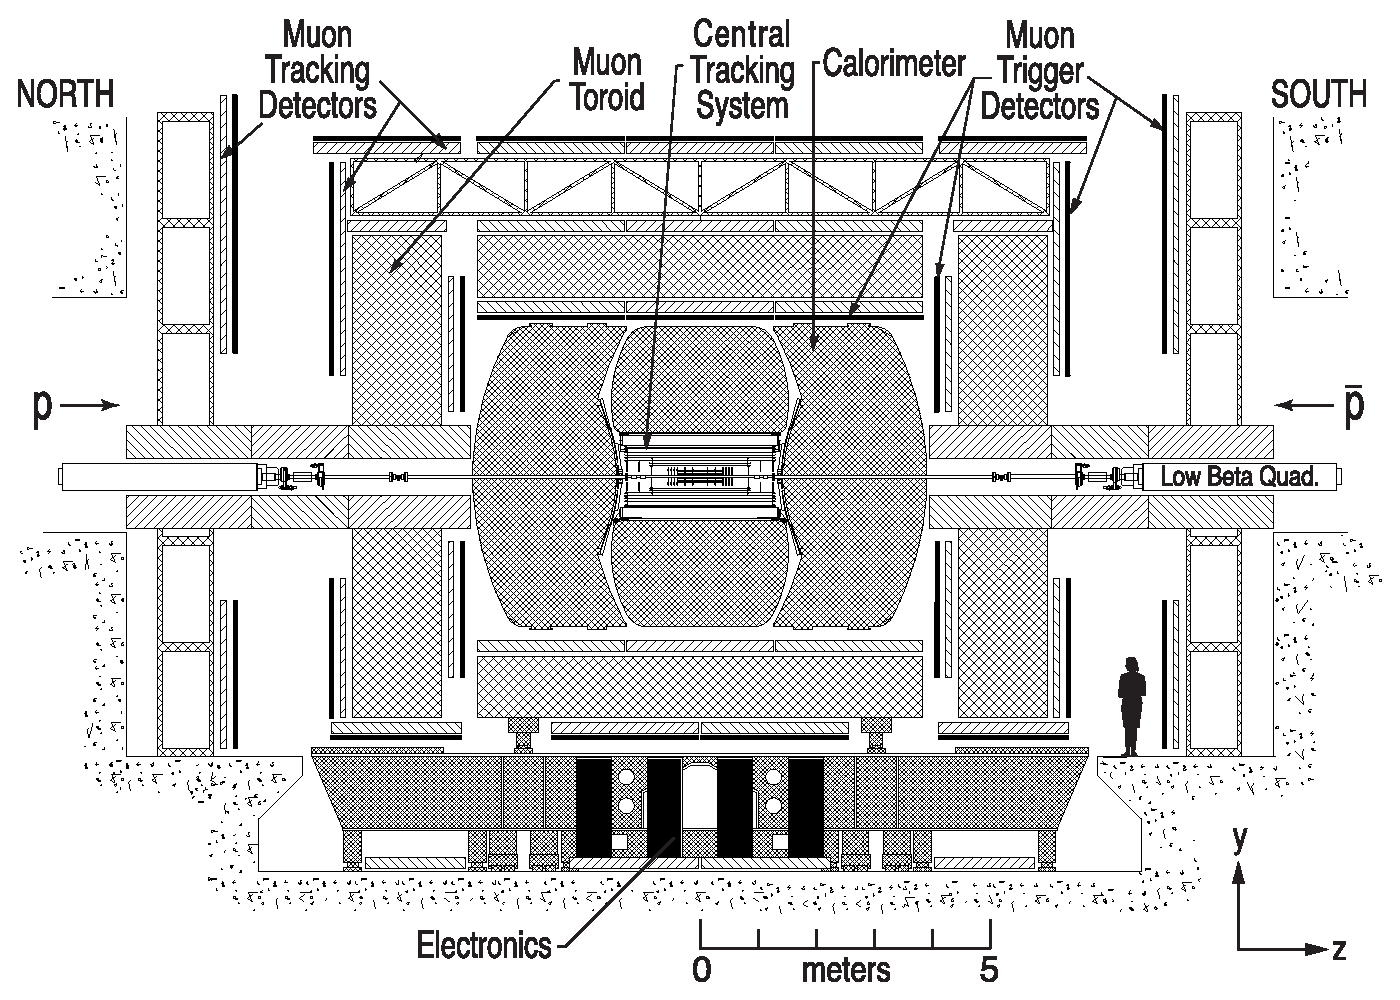
\includegraphics[width=1.0\textwidth]{eps/D0/DetectorSlice.eps}
\end{center}
\vspace{-0.1in}
\caption{Schematic side-view of the $\dzero$~detector~\cite{Abazov:2005pn}.}
\label{D0}
\end{figure}

\subsection{Tracking Detectors}
\label{tracking}

The innermost layer of the $\dzero$~detector is a set of two tracking detectors designed to measure the flight path of charged particles. The two detectors, shown in Fig.~\ref{InnerDetector}, are the silicon microstrip tracker (SMT) and the central fiber tracker (CFT). The SMT and CFT are located within a 2T magnetic field generated by a superconducting solenoid magnet. The presence of the magnetic field within the tracking detectors will deflect all charged particles allowing a measure of the their charge and momentum through the sign and radius of the induced curvature.

\begin{figure}[!h!tbp]
\begin{center}
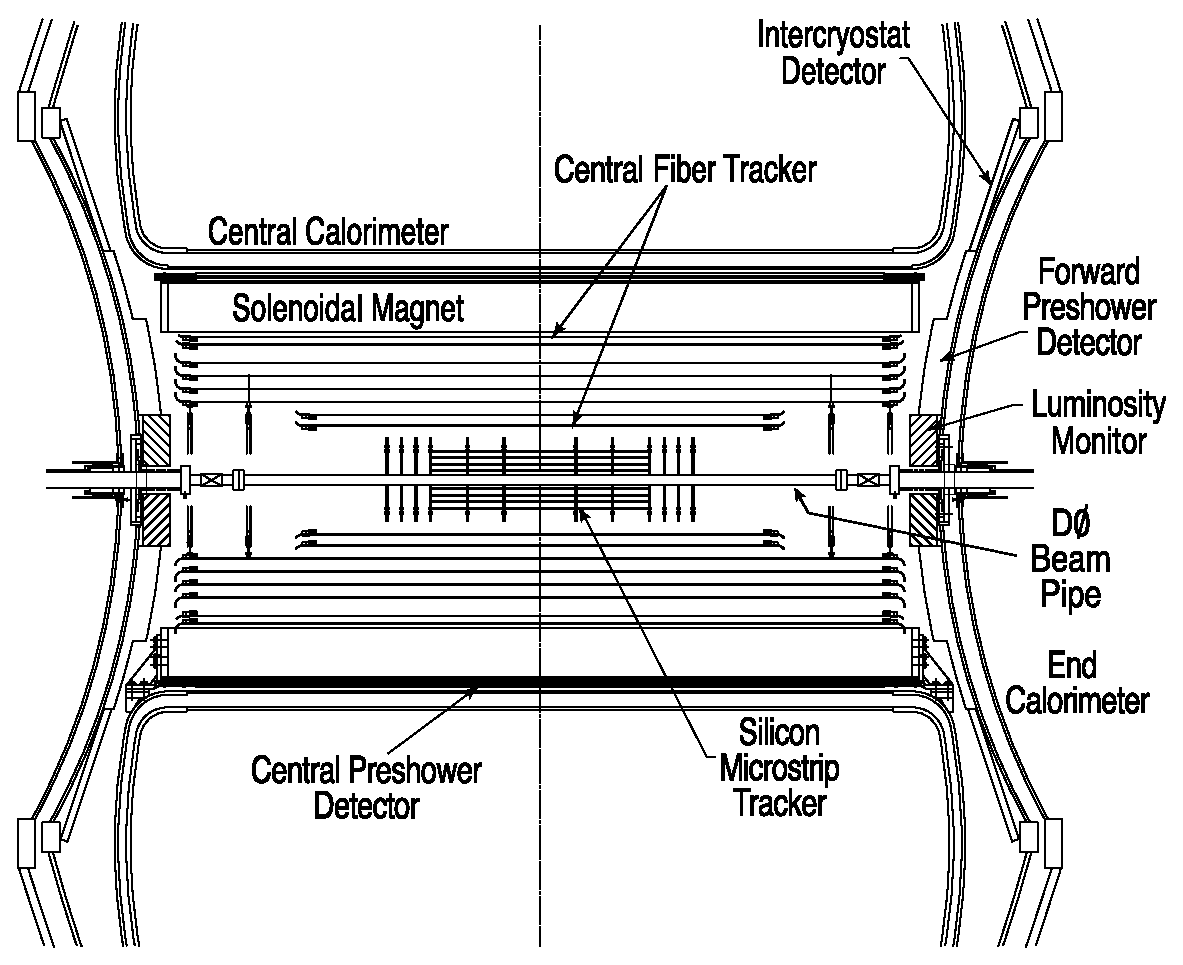
\includegraphics[width=0.75\textwidth]{eps/D0/InnerDetector.eps}
\end{center}
\vspace{-0.1in}
\caption{Schematic of the two tracking detectors (SMT and CFT) as well as the superconducting solenoid magnet~\cite{Abazov:2005pn}.}
\label{InnerDetector}
\end{figure}

\subsubsection{Silicon Microstrip Tracker}

The SMT is located immediately outside the Tevatron beam pipe and is designed to provide high resolution position measurements of charged particles. The SMT is a collection of doped silicon detectors depleted of electric charge by the application of a reverse bias voltage. As a charged particle enters the depleted region it ionizes the silicon creating electron-hole pairs. The result of the applied electric field is to force the charges to drift towards active sensors. The typical drift distance for charges in the silicon is $300$~$\mu$m. A schematic of the SMT is shown in Fig.~\ref{SMT}.

\begin{figure}[!h!tbp]
\begin{center}
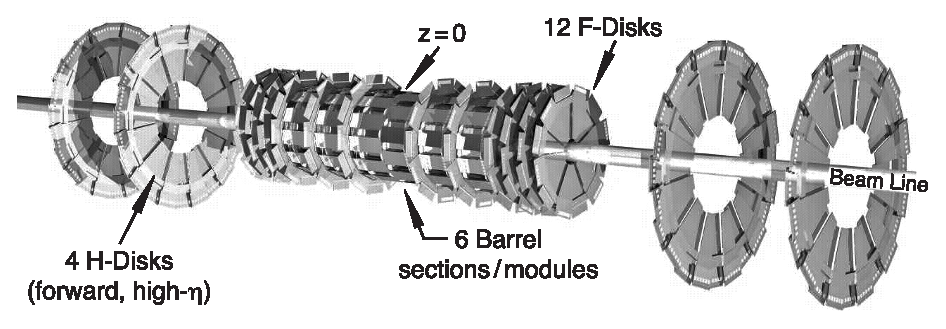
\includegraphics[width=0.75\textwidth]{eps/D0/SMT.eps}
\end{center}
\vspace{-0.1in}
\caption{Schematic of the silicon microstrip tracker sub-detector~\cite{Abazov:2005pn}.}
\label{SMT}
\end{figure}

The geometry of the SMT is dictated by the length of the interaction region\footnote{The typical Gaussian width of the hard scatter interactions is $25$~cm centered around z=0.} and a desire to maximize the number of layers a charge particle traverses. To achieve this goal the detector is organized into three structures: the barrel detector, the F-discs, and the H-discs. The barrel detector is a set of six barrels concentric with the beam pipe that each contain four double-sided layers of silicon wafers. The barrels provide coverage for centrally produced charged particles with $|\eta|<1.1$. The F-discs are also double-sided silicon wafers. These silicon detectors are oriented perpendicular to the beam axis in contrast with the concentric barrels. There are twelve F-disks in the SMT, six in the central region that cap each barrel and six in the forward region. The SMT also has four silicon detectors at high $|z|$ called H-disks, which are oriented perpendicular to the beam axis. In total the SMT has 912 individual readout modules and nearly 800,000 individual readout channels.


\subsubsection{Central Fiber Tracker}

Immediately outside of the SMT is the central fiber tracker (CFT) which occupies the radial distance of 20 to 52 cm from the beam pipe. The CFT is organized into 8 layers of scintillating fibers which produce light when a charged particle traverses the fibers. Each layer of the CFT consists of two sets of fibers: one that is parallel with the beam axis and one that is rotated $3^{\circ}$ with respect to the beam axis. 
The fibers in the tracker are $835$~$\mu$m in diameter and composed of organic scintillating compounds surrounded by a thin layer of cladding designed to provide total internal reflection inside the fiber. The light produced in the fiber is carried out of the detector by wave guides with typical travel distances between 8 and 11 m. Because the light is only read out at one end of the fiber the other end is coated with sputtered aluminum which reflects 90$\%$ of the light back to the end which is read out. An endview schematic of the CFT layers and their associated waveguides is shown in Fig.~\ref{CFT}.  Light produced in the CFT is recorded on silicon avalanche photon counters called VLPCs (visible light photon counter). The VLPCs operate at $9^{\circ}$~K to reduce thermal noise and achieve a quantum efficiency of $75\%$.

\begin{figure}[!h!tbp]
\begin{center}
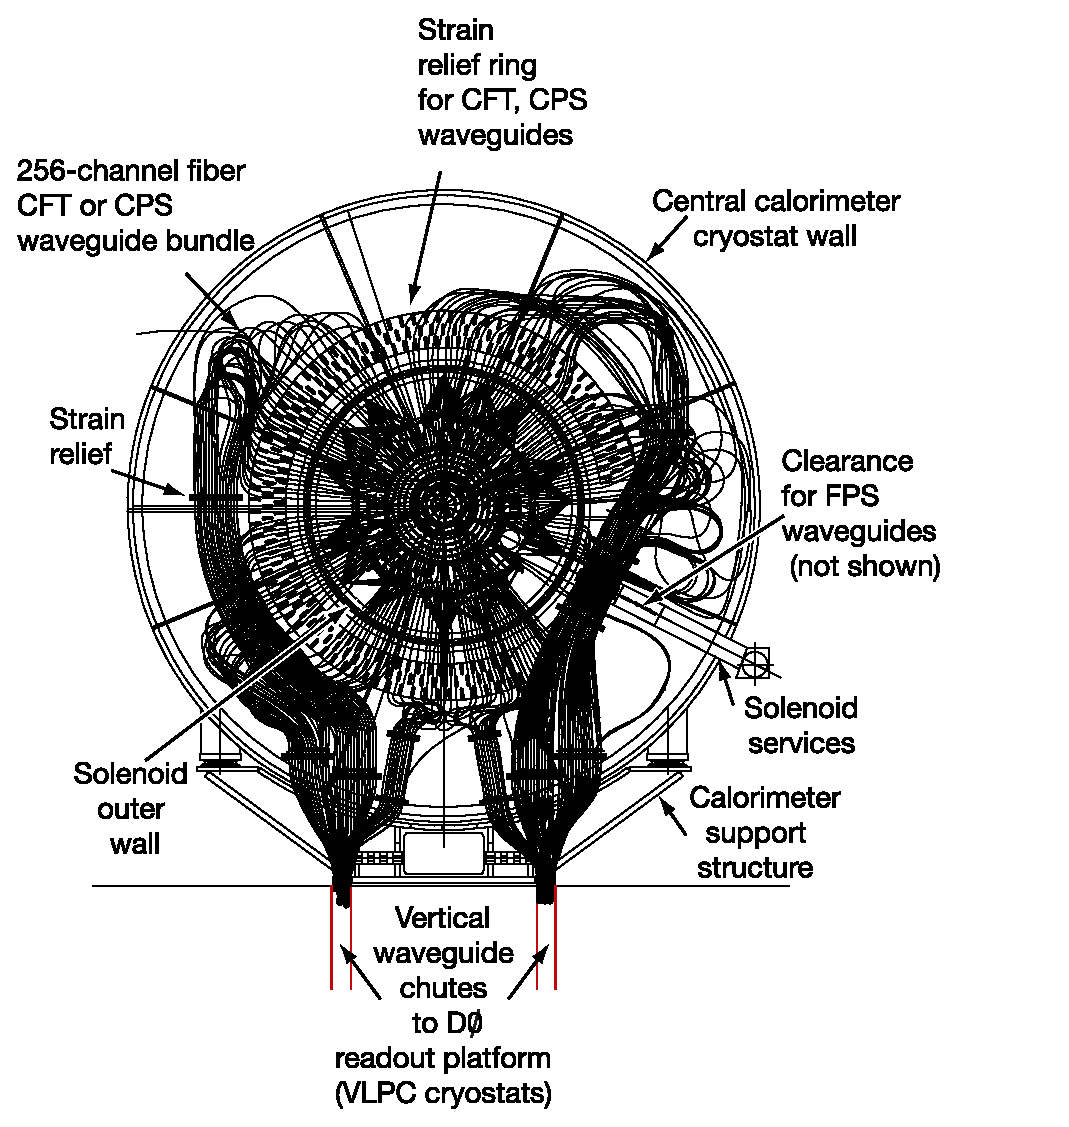
\includegraphics[width=0.75\textwidth]{eps/D0/CFT.eps}
\end{center}
\vspace{-0.1in}
\caption{Schematic endview of the central fiber tracker with corresponding waveguides~\cite{Abazov:2005pn}.}
\label{CFT}
\end{figure}

\subsection{Calorimetry}
\label{calorimetry}

The next layer of the $\dzero$~detector is the calorimeter. The calorimeter is designed to measure the energy of electromagnetically interacting particles such as electrons and photons as well as strongly interacting particles such as pions and neutrons. The $\dzero$~calorimeter is divided into three sub-detectors: one central region (CC) and two end-cap regions (EC) as seen in Fig.~\ref{Calorimeter}. Each region is encased in its own cryostat held at a constant temperature of $90^{\circ}$~K. The region between the two cryostats, $0.8 < |\eta| < 1.4$, is called the inner cryostat region (ICR) and contains active scintillator to provide a minimal energy measurement in this region.

\begin{figure}[!h!tbp]
\begin{center}
\includegraphics[width=0.75\textwidth]{eps/D0/Calorimeter.eps}
\end{center}
\vspace{-0.1in}
\caption{3D view of the $\dzero$ calorimeter~\cite{Abazov:2005pn}.}
\label{Calorimeter}
\end{figure}

Each detector region, except the ICR, measures energy using a similar approach by inducing the incoming particles to produce an electromagnetic shower as they collide with a dense material. As particles from the shower enter the active region they will ionize the material. The ions in the active material move towards a sensor due to an applied bias voltage. The amount of charge collected on the sensor is then proportional to the energy deposited by the ionizing particle. An example of an electromagnetic shower originating from a photon is shown in Fig.~\ref{EMshower}.  The typical ion drift time in the $\dzero$~calorimeter is $\sim450$~ns.


\begin{figure}[!h!tbp]
\begin{center}
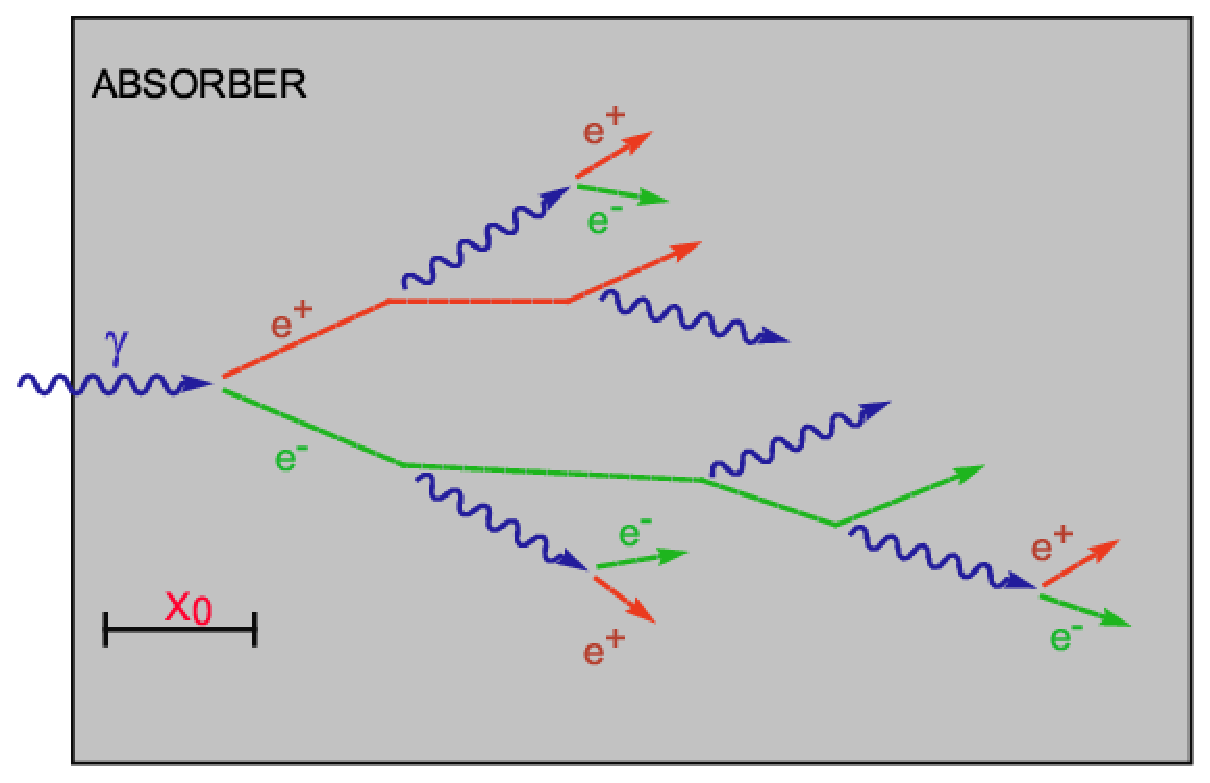
\includegraphics[width=0.75\textwidth]{eps/D0/shower.eps}
\end{center}
\vspace{-0.1in}
\caption{Initial stages of an electromagnetic shower caused by a photon interacting with an absorber material. The radiation length $x_{0}$ is the typical distance a photon will travel before producing an $e^{+}e^{-}$ pair or the distance before an electron will radiate a photon~\cite{shower}.}
\label{EMshower}
\end{figure}

The $\dzero$ calorimeter consists of an inner detector called the EM calorimeter and an outer detector called the hadronic calorimeter. The EM calorimeter is constructed of alternating layers of depleted Uranium, which acts as the shower inducing material, and liquid Argon, which acts as the active medium. The depleted Uranium plates are 3 mm thick in the central region and 4 mm thick in the forward end-cap region while the liquid Argon active region is 2.3 mm thick. An cartoon drawing of this arrangement can been seen in Fig.~\ref{CalorimeterCell}. The EM calorimeter has four layers of cells representing nearly 21 radiation lengths. The hadronic calorimeter is actually two detectors: one called the fine hadronic calorimeter which employs 6 mm thick Ur-Ni alloy as the shower inducing material and the coarse hadronic calorimeter which uses 46.5 mm thick plates of copper in the central region and stainless steel in the forward region. The hadronic calorimeter also uses liquid Argon as the active material. The combination of the fine and coarse hadronic calorimeters provides an additional 7 radiation lengths to the detector. The numerous radiation lengths are important to ensure that a particle deposits nearly all of its energy in the detector.


\begin{figure}[!h!tbp]
\begin{center}
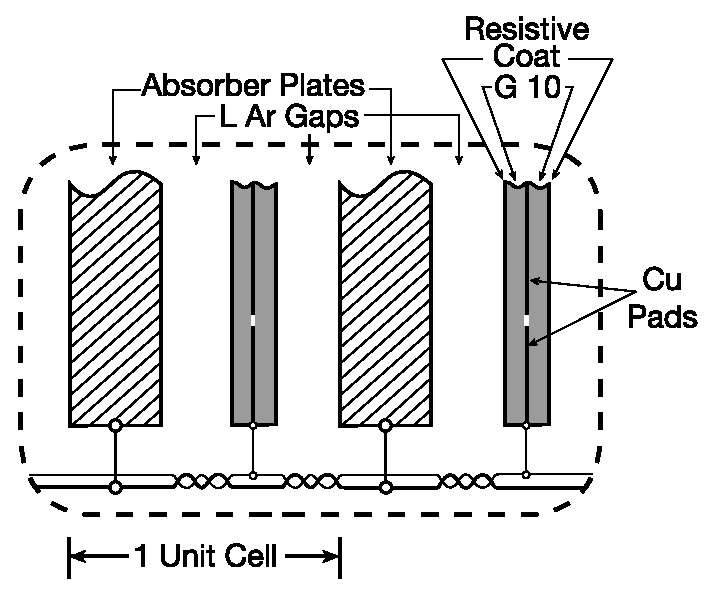
\includegraphics[width=0.75\textwidth]{eps/D0/CalorimeterCell.eps}
\end{center}
\vspace{-0.1in}
\caption{Example of a typical calorimeter cell of alternating absorber and active material. Particles traverse the calorimeter cell from left to right in this diagram~\cite{Abazov:2005pn}.}
\label{CalorimeterCell}
\end{figure}

The $\dzero$~calorimeter also has fine segmentation (i.e. radial size of the cells), which allows for excellent energy and position measurement of particles as they shower in the detector. The segmentation of the EM calorimeter in $\delta\eta \times \delta\phi$ is $0.1 \times 0.1$ for all layers except the third layer, where the segmentation is $0.05 \times 0.05$. The fine segmentation in the third layer 
is because the electromagnetic shower is expected to reach a maximum in this layer. The fine hadronic layers of the calorimeter also have a segmentation of $0.1 \times 0.1$, while the segmentation in the coarse hadronic calorimeter is $0.2 \times 0.2$. An octant of the $\dzero$~calorimeter including segmentation can be seen in Fig.~\ref{CalorimeterSegmentation}. 

\begin{figure}[!h!tbp]
\begin{center}
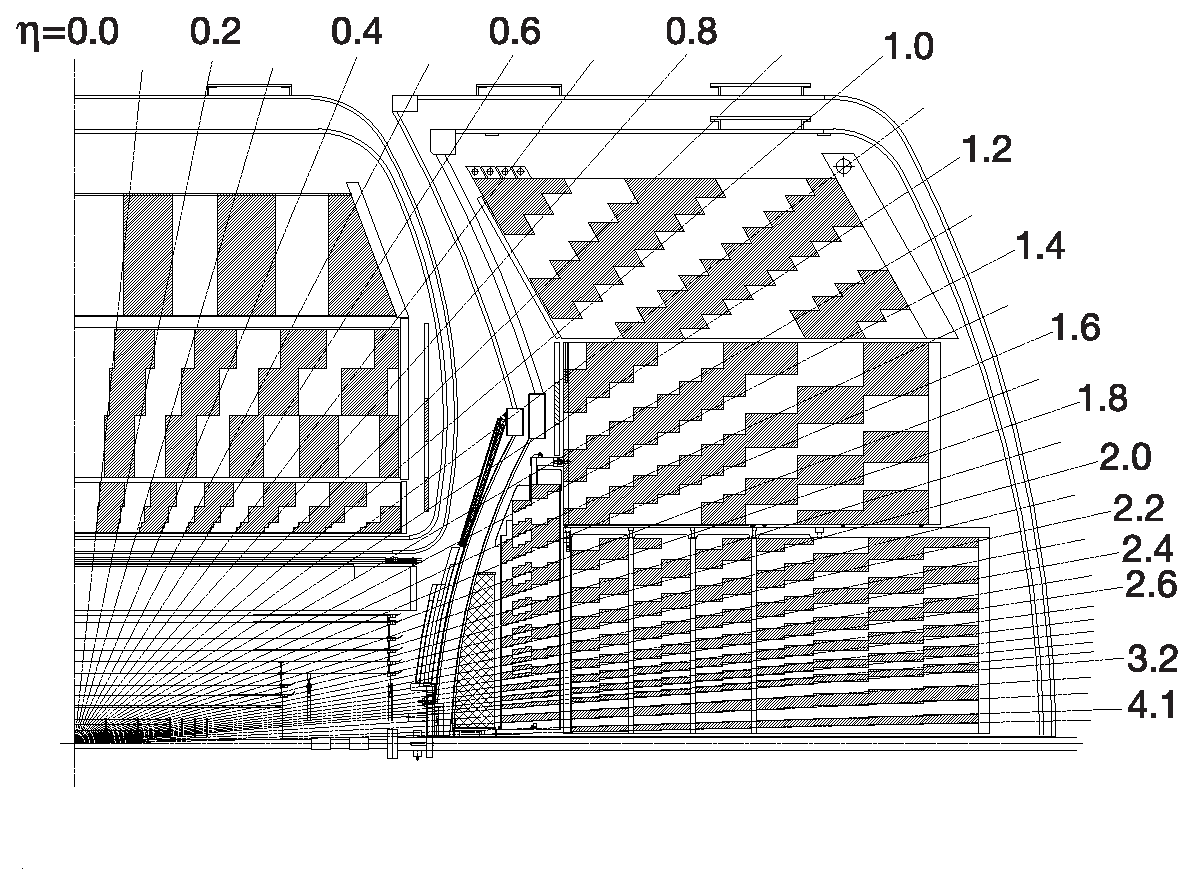
\includegraphics[width=0.75\textwidth]{eps/D0/CalorimeterSegmentation.eps}
\end{center}
\vspace{-0.1in}
\caption{Octant of the $\dzero$~calorimeter. The fine segmentation of the calorimeter is clearly seen in this diagram~\cite{Abazov:2005pn}. The alternating dark and light blocks represent cells in different calorimeter towers.}
\label{CalorimeterSegmentation}
\end{figure}



\subsection{Luminosity Monitor}
\label{luminositydetector}

Located directly in front of the end-cap calorimeters, covering a $\eta$ range between 2.7 and 4.4, is the luminosity monitor, which collects information about inelastic $\ppbar$~collisions for each bunch crossing. The luminosity monitor is a set of 24 plastic scintillators which can detect low angle (high $\eta$) fragments from the break-up of the protons in the $\ppbar$~collision. The scintillators produce light when the charged fragments traverse the detector and that light is recorded by photo-multiplier tubes. A schematic of the luminosity monitor is shown in Fig.~\ref{Luminosity}.

\begin{figure}[!h!tbp]
\begin{center}
\includegraphics[width=0.75\textwidth]{eps/D0/Luminosity.eps}
\end{center}
\vspace{-0.1in}
\caption{Schematic of the $\dzero$ luminosity monitor shown in relation to the beam pipe, SMT, and endcap calorimeter~\cite{Abazov:2005pn}.}
\label{Luminosity}
\end{figure}


Collecting information about inelastic collisions is vital to properly normalize all data collected at $\dzero$. The luminosity monitor is designed to measure the inelastic $\ppbar$~cross section, which is a quantity that is known from measurements by previous experiments. By measuring the inelastic $\ppbar$~cross section the total integrated luminosity to which the $\dzero$~detector has been exposed to can be measured~\cite{d0note4958,d0note5139}. A derivation of the luminosity from the measured $\ppbar$~inelastic cross section can be found in Appendix~\ref{lumi}.

Along with providing a luminosity measurement, the detector also acts as a fast vertex finder. By measuring the relative difference of coincidence counts in the North and South detectors the $z$ position of the vertex can be determined from Eq.~\ref{zpos}, where $t_{\pm}$ are the time measured by the North (+) and South (-) detectors, respectively. The time of flight resolution for the luminosity detector is 0.3 ns.

\begin{equation}
\label{zpos}
z = \frac{c}{2}(t_{+} - t_{-})
\end{equation}

\subsection{Muon Detector}
\label{muondetector}

The outer-most layer of the $\dzero$~detector is the muon system. A special detector is required to measure muons because they do not deposit much energy in the tracker or calorimeter and thus a confirmation of their presence using these sub-detectors alone is difficult to infer. The muon detector has two active regions called the central region for $|\eta|<1$ and the forward region for $1<|\eta|<2$. The system also employs a 2 T toroid iron magnet to bend the muons from their original paths. The addition of the magnetic field helps to provide a local momentum measurement in the event the momentum can not be determined from the tracking detector. Additional shielding surrounding the beam pipe near the forward muon detector is designed to reduce spurious beam effects which dramatically reduces the amount of radiation to which to detector is exposed. A schematic of the muon system and the beam shielding can be seen in Fig.~\ref{MuonDetector}.

\begin{figure}[!h!tbp]
\begin{center}
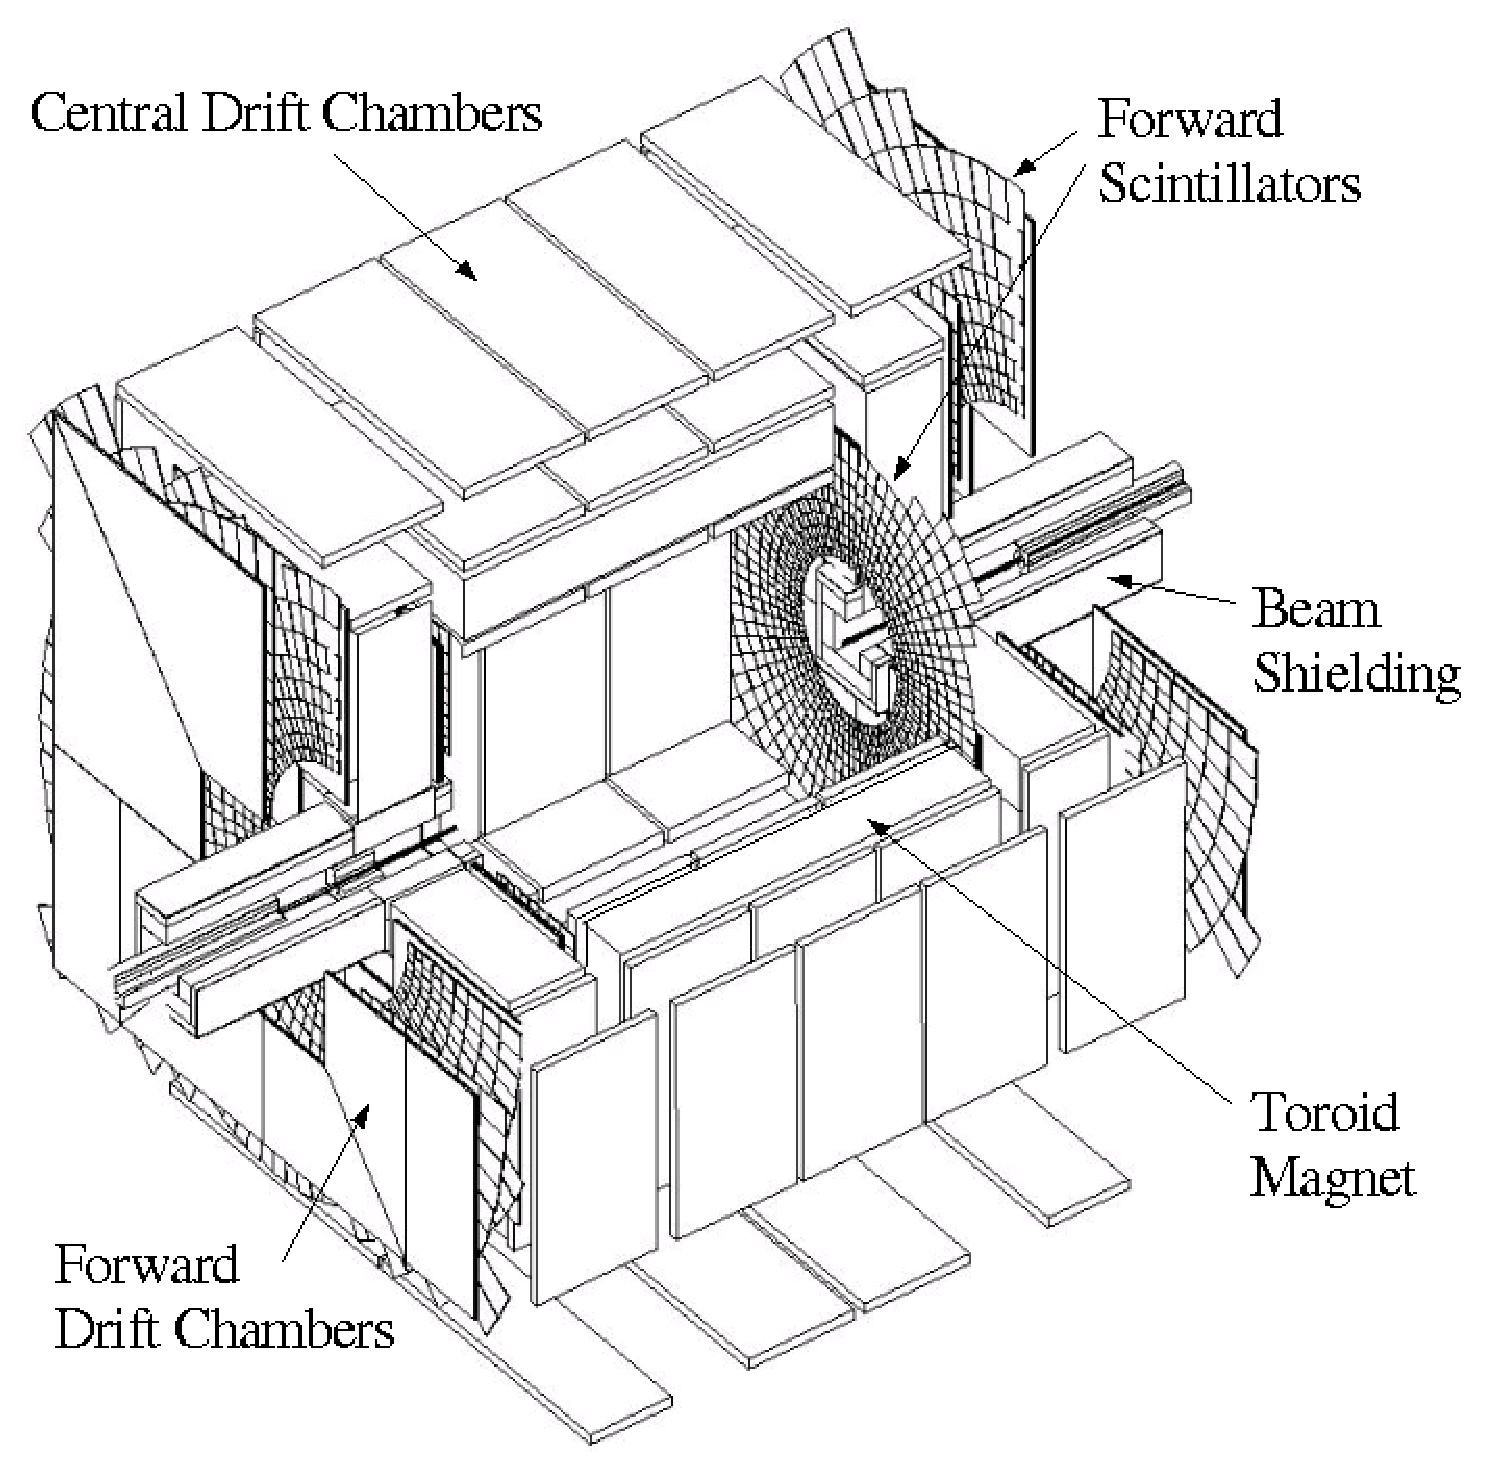
\includegraphics[width=0.75\textwidth]{eps/D0/mudet.eps}
\end{center}
\vspace{-0.1in}
\caption{3D view of the $\dzero$ muon detector~\cite{Abazov:2005pn}.}
\label{MuonDetector}
\end{figure}

The muon system at $\dzero$ is a three layer detector, both in the central and forward regions, consisting of drift chambers for precise position measurement and scintillator counters for muon identification and fast triggering (Section~\ref{triggersystem}). The scintillator counters produce light when the muon passes through the detector which is then collected by a photo-multiplier tube. The drift chambers have a central wire held at a large voltage surrounded by an inert gas. As the muon enters the chamber it will ionize the gaseous organic compound mixture and the resulting free charges will drift towards the wire. The position of the muon is found by analyzing the current profile in the wire. In the central region the drift chambers are called PDTs (proportional drift tubes) and are rather large with typical areas of 2.8 $\times$ 5.6 m$^{2}$. The forward region uses smaller drift chambers called MDTs (mimi drift tubes), which are a collection of eight cells of size 9.4 $\times$ 9.4 mm$^{2}$. The position resolution of the drift chambers is $\sim$1 mm.

\subsection{Trigger and Data Acquisition System}
\label{triggersystem}

The previous sections in this chapter describe how the $\dzero$~detector collects information from $\ppbar$~collisions at the Tevatron, which occur every $396$~ns. While $\dzero$ records information about every collision, it does not save every event to tape for two reasons: most collisions at the Tevatron are small angle inelastic collisions which have already been well studied and the total rate of data one can reliably store to tape is limited to $\sim$30MB/s. Because $\dzero$~can not save every event, a sophisticated trigger system is employed to reduce the total rate to tape to $50$~Hz. This trigger system attempts to select the most ``interesting" events, which will be used for an analysis or future calibration of the detector.

The trigger system is comprised of three independent stages called level 1, level 2, and Level 3, which are designed to reduce the total event rate from $1.7$~MHz to $50$~Hz. A schematic of the combined trigger system is shown in Fig.~\ref{Trigger}. The level 1 system is composed of hardware trigger elements and has the goal of reducing the initial rate of  $1.7$~MHz to $1.5$~kHz. Because the level 1 trigger must act quickly to either accept or reject an event, the tools available for selecting interesting events is limited. At level 1 only calorimeter trigger towers, which are layers of calorimter cell energies within a $\delta\eta \times \delta\phi = 0.2 \times 0.2$ space, signals in the muon drift chambers or scintillators, and the transverse momentum of charged particle tracks in the central fiber tracker are available for trigger decisions.

\begin{figure}[!h!tbp]
\begin{center}
\includegraphics[width=0.75\textwidth]{eps/D0/TriggerFlow.eps}
\end{center}
\vspace{-0.1in}
\caption{Cartoon drawing of the $\dzero$ trigger system~\cite{Abazov:2005pn}.}
\label{Trigger}
\end{figure}

The level 2 trigger acts on all events which pass the level 1 trigger and is designed to reduce the rate from 1.5kHz to $700$Hz. The level 2 trigger uses detector specific pre-processing boards and a global detector board to make trigger decisions. The pre-processors collect data from the level 1 trigger system as well as readout information from the individual detectors. The pre-processors use this information to form physics objects such as electrons, jets, and missing E$_{T}$\footnote{Physics objects and event-wide kinematic variables such as missing E$_{T}$~are fully described in Chapter~\ref{EventSelection}.}. A global level 2 pre-processor uses all the information from the sub-detector pre-processors to make trigger decisions based on event-wide kinematics.

The next stage in the trigger selection process is the level 3 trigger, which is a software-based collection of algorithms executed on a collection of computer farm nodes. The goal of the level 3 trigger is to reduce the data rate to tape from $700$~Hz to $50$~Hz. The level 3 trigger requires the full detector readout to select events, thus all sub-detector data must be transmitted to the farm nodes. A level 3 data acquisition system was designed to transmit data over ethernet cables to the farm nodes. Upon a level 2 trigger accept a controller card in the sub-detector VME crate signals to a single board computer\footnote{The single board computers used in this DAQ are VMIC 7750 with a 933 MHz Pentium-III processor, 128 MB of RAM, 128  MB of on-board flash memory, and two 100 MB/s ethernet connectors. A few of the CFT crates use 2-1GB/s ethernet connector due to the high event sizes for these crates.}, located in the VME crate, to begin collecting the crate data and store it in RAM memory located on the SBC. While the data is being collected by the SBCs, a dedicated SBC called the Routing Master is collecting information about the event number as well as the level 1 and level 2 triggers that initially selected the event. The Routing Master communicates with the level 3 computer farm regarding its availability (i.e. if it is busy processing events or waiting for a new event) and assigns each event a unique farm node to which all SBCs must send the event information. This process is repeated for each event which is selected by the level 2 trigger. When the SBC has the full crate data stored in memory and a routing command issued by the Routing Master, the crate data is transmitted via one of two $100$~MB/s ethernet cables to the farm nodes.

Each event that is selected by the level 2 trigger ranges in size from 250 to 300~kB resulting in 200-300 MB/s of data being sent to the farm nodes. To handle this enormous data transfer rate, a set of CISCO 2948G ethernet switches concentrate ten 100~MB/s connections into a 1 GB/s optical fiber. The GB fibers are then brought to a CISCO 6509 ethernet switch capable of transmitting data at a rate of 16 GB/s. A schematic of this hardware setup and the data flow are shown in Fig.~\ref{l3all}.

\begin{figure}[!h!tbp]
\begin{center}
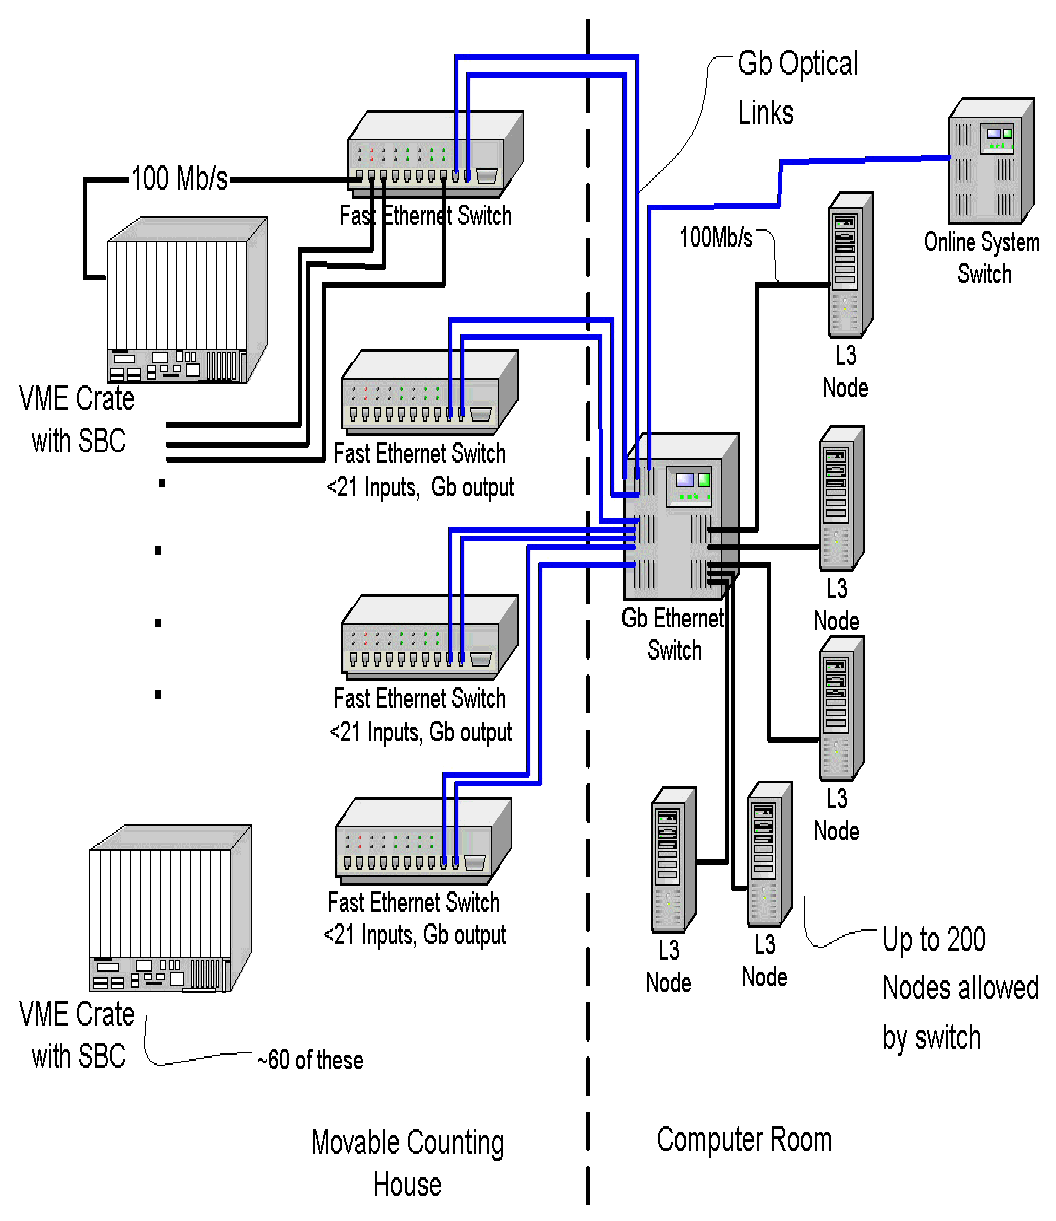
\includegraphics[width=0.49\textwidth]{eps/Level3/L3-DAQ.eps}
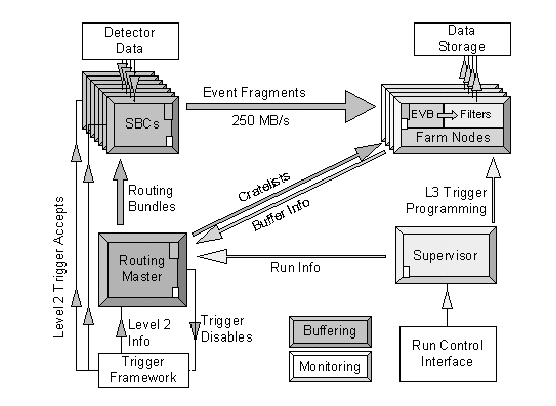
\includegraphics[width=0.49\textwidth]{eps/Level3/daq_software.eps}
\vspace{-0.1in}
\caption{Experimental setup of the level 3 trigger and data acquisition system (left) and the flow of data through the system (right).}
\label{l3all}
\end{center}
\end{figure}

When the data arrives at a farm node it is processed by a programmed called the Event Builder. This software package combines event fragments from each sub-detector data and organizes them into a readable format for the level 3 trigger software. If the Event Builder does not receive data from all sub-detector crates within a one second window after receiving the first fragment the event is dropped. As stated earlier the Event Builder transmits the number of events it is currently processing to the Routing Master, allowing this software to choose farm nodes based on availability. Finally, between two and four level 3 trigger processes examine the event to see if it satisfies at least one of the trigger criteria. Events which pass the level 3 trigger are sent over 100 MB/s ethernet for temporary storage on a machine called the Collector. When enough events are accumulated the data is stored on a machine called the Datalogger and finally to tape storage at the Feynman Computing Center located at Fermilab.

% ========== Chapter 4

\chapter{Event Reconstruction And Simulation}
\label{EventSelection}
\label{recosim}

An important step in any high energy physics analysis is to reconstruct the hard scatter collision from the small deposits of energy measured in the detector. This chapter describes how each sub-detector is used to reconstruct a physics object, such as an electron or muon, which can be used to classify the event as signal or background. Section~\ref{reconstruction} of this chapter describes how electrons, muons, and calorimeter jets are reconstructed in data and Monte Carlo simulated events. Reconstruction of Monte Carlo events requires simulating the $\dzero$~detector such that each Monte Carlo event reproduces the detector resolution observed in data events. The $\dzero$~detector and trigger simulation is described in Sections~\ref{simulation} and~\ref{triggersim}, respectively. Finally, to correct for inevitable un-modeled effects in the simulation, correction factors must be applied to the Monte Carlo. The measurement of these factors and how they are applied is given in Section~\ref{corrections}.

\section{Object Reconstruction}
\label{objectreco}

The following section describes how physics objects are reconstructed using quantities measured in the detector. Section~\ref{trackreco} describes how charged particle tracks are identified through small energy deposits in the central tracking detectors. Once all tracks have been identified the primary interaction vertex can be reconstructed as described in Section~\ref{pvreco}. Electrons and muons are identified through a series of quality cuts as described in Sections~\ref{electronreco} and~\ref{muonreco}, respectively. Section~\ref{jetreco} explains how jets are identified from showers of electromagnetic and hadronic particles in the calorimeter. Once jets, electrons, and muons have been identified the missing transverse energy can be calculated as the $p_{T}$ imbalance in the event as described in Section~\ref{metreco}. Finally, identification of heavy flavor jets using a neural network is described in Section~\ref{bidreco}.

\label{reconstruction}
\subsection{Tracks}
\label{trackreco}

A track represents the three dimensional path of a charged particle as it traverses the detector. In the presence of a magnetic field, such as the case with the inner $\dzero$~detectors, all electrically charged particles move in a helical trajectory. Five parameters are needed to fully parameterize the helix and it is the task of the track finding algorithms to measure these parameters for all charged particles.

The first step in constructing a track is to form ``hits" where ionizing particles have deposited energy in the tracking detectors. The formation of track hits is described in the $Track~Hit~Clustering$~section below. Once the track hits have been created two algorithms are employed to link them together to create charged particle tracks. The two algorithms are described in the $Histogramming~Track~Finding~Method$ and $Alternative~Algorithm$ sections below. A final set of reconstructed tracks is formed by a global track reconstruction algorithm that combines the tracks found by the two previously mentioned algorithms.

\subsubsection{Track~Hit~Clustering}

Building a track begins with forming hits in both the SMT and CFT tracking detectors. A hit in the SMT detector is characterized by the deposition of energy in a silicon strip left by an ionizing particle. If the resulting collected charge is above threshold (to reduce noise hits), a hit is registered. If an adjacent silicon strip also registers a hit the two hits are combined. This process is repeated for any adjacent strip which registers a hit. The center of the SMT hit is given by the charge weighted average of the central position of each silicon strip\footnote{Because the SMT detector is immersed in a magnetic field the electron-positron pairs created in the silicon will drift at an angle with respect to electric field lines within the silicon. This angle, known as the Lorentz angle, is corrected for when calculating the center of the SMT hit.}. A hit in the CFT is formed when two fibers in each super layer register scintillation light indicating the presence of a charge particle traversing the fibers. Because the fibers have a relative $3^{\circ}$~orientation, the $x-y$~coordinates are calculated as the intersection of two scintillating fibers. 

\subsubsection{Histogramming Track Finding Method (HTF)}
\label{htf}

The histogramming track finding (HTF)~\cite{htf} method is based on the principle that a particle which produces many hits in the transverse plane (x-y) will have a unique curvature and azimuthal angle. This method transforms (x-y) hits in the SMT and CFT and into a new plane defined by the curvature, $\rho$, and azimuthal angle, $\phi$. Hits from the same particle will produce a peak in the $\rho-\phi$~space, whereas random hits will uniformly populate the space. An example of this procedure, known as a Hough transformation, for a 1.5~GeV muon track is shown in Fig.~\ref{histogramming}. A histogram is created of the hits in the new $\rho-\phi$ space and is processed through a two-dimensional Kalman filter, which attempts to remove "noisy" tracks with large track errors as well as incorporate detector geometry and material density. The result of the filter is a set of smoothed tracks whose track parameters have been re-fit with smaller errors. The longitudinal coordinate information is included by creating a new histogram in a space defined by the radial distance to the beam axis and the $z$~coordinate. A second Hough transformation is performed into the $(z_{0},C)$ plane, where $z_{0}$ is the intersection of the track along the beam axis and $C$ is the track inclination defined as $\frac{dr}{dz}$. The newly formed tracks are extrapolated either inward toward the SMT if the track finding began in the CFT or outward toward the CFT if the track finding began in the inner SMT detector.

\begin{figure}[!h!tbp]
\begin{center}
\includegraphics[width=0.75\textwidth]{eps/Reco/htf.eps}
\end{center}
\vspace{-0.1in}
\caption{This histogramming track finding technique shown for an example of a single 1.5 GeV track of 5 hits. (a) The family of trajectories containing a given hit. (b) The geometric place of all trajectories containing a given hit in parameters space. (c) Curves from different hits intersect at one point corresponding to the track parameters. (d) The point of intersection can be seen as a peak in the ($\rho$,~$\phi$) histogram~\cite{htf}.}
\label{histogramming}
\end{figure}


\subsubsection{Alternative Algorithm Tracking (AA)}
\label{aa}

The alternative algorithm (AA)~\cite{aa} track finding method is based on a seed hit in one layer of the detector and building a track by incrementally including more layers of the SMT and CFT detectors. The algorithm takes SMT hits in the innermost layers and adds additional layers if the resulting extrapolated track radius of curvature is greater than $30$~cm, which indicates the track must have $p_{T}>180$~MeV. All possible combinations that meet these requirements are stored. The algorithm also allows for missing hits in the SMT or CFT if a hit in one of the outer layers is consistent with a previously found track. Also allowed are ``CFT-only" tracks built from seeds in the CFT detector that have less than 3 hits in the SMT detector. Allowing tracks to be built in this manner dramatically increases the overall track finding efficiency of the algorithm.


\subsection{Primary Interaction Vertex}
\label{pvreco}

The primary interaction vertex is defined as the three-dimensional location of the hard scatter interaction. The hard scatter interaction vertex is very important to locate to allow discrimination of physics objects resulting from the $\ppbar$~collision and objects created from noise in the detector or other low energy inelastic $\ppbar$~collisions.

Primary interaction vertices are found using the adaptive primary vertex algorithm~\cite{pv}. This algorithm attempts to assign all tracks with $p_{T}>0.5$~GeV and at least two SMT hits to a vertex where the extrapolated track paths intersect. The result of this first pass fit to the primary vertex is a $\chi^{2}$ for each track hypothesis. The algorithm then attempts a second pass fit to the primary vertex except this time each track receives a weight, shown in Eq.~\ref{pvweight}, that includes the $\chi^{2}$ of the previous track fit.

\begin{equation}
\label{pvweight}
w_{i} = \frac{1}{1+e^{(\chi^{2}_{i} - \chi^{2}_{\rm{cutoff}})/2T}}
\end{equation}

\noindent Where the values for $\chi^{2}_{\rm{cutoff}}$ and T are 16 and 4, respectively. The vertex fitting procedure is repeated until the difference of weights from the previous iteration for each track is less than $10^{-4}$.

The adaptive vertexing algorithm produces a list of possible vertices of which one might be the hard scatter vertex. To determine which vertex is the hard scatter vertex all tracks are assigned a probability to not originate from the hard scatter vertex. This probability, shown in Eq~\ref{trackpv}, is based on the $\log_{10}(p_{T})$ (~F$(p_{T})$~)~distribution for tracks associated with a minimum bias\footnote{A minimum bias vertex is a vertex from an inelastic $\ppbar$~collision.} interaction as determined from Monte Carlo simulation.

\begin{equation}
\label{trackpv}
P(p_{T}) = \frac{\int_{\log_{10}(p_{T})}^{\infty} F(p^{'}_{T})dp^{'}_{T}}{\int_{\log_{10}(0.5)}^{\infty} F(p^{'}_{T})dp^{'}_{T}}
\end{equation}

The individual track probabilities are combined for each track associated to each vertex found by the adaptive vertex algorithm to form a minimum bias vertex probability. The vertex which has the lowest minimum bias probability is selected as the hard scatter vertex. The distribution of this probability for minimum bias and hard scatter vertices is shown in Fig.~\ref{minimum bias}.

\begin{figure}[!h!tbp]
\begin{center}
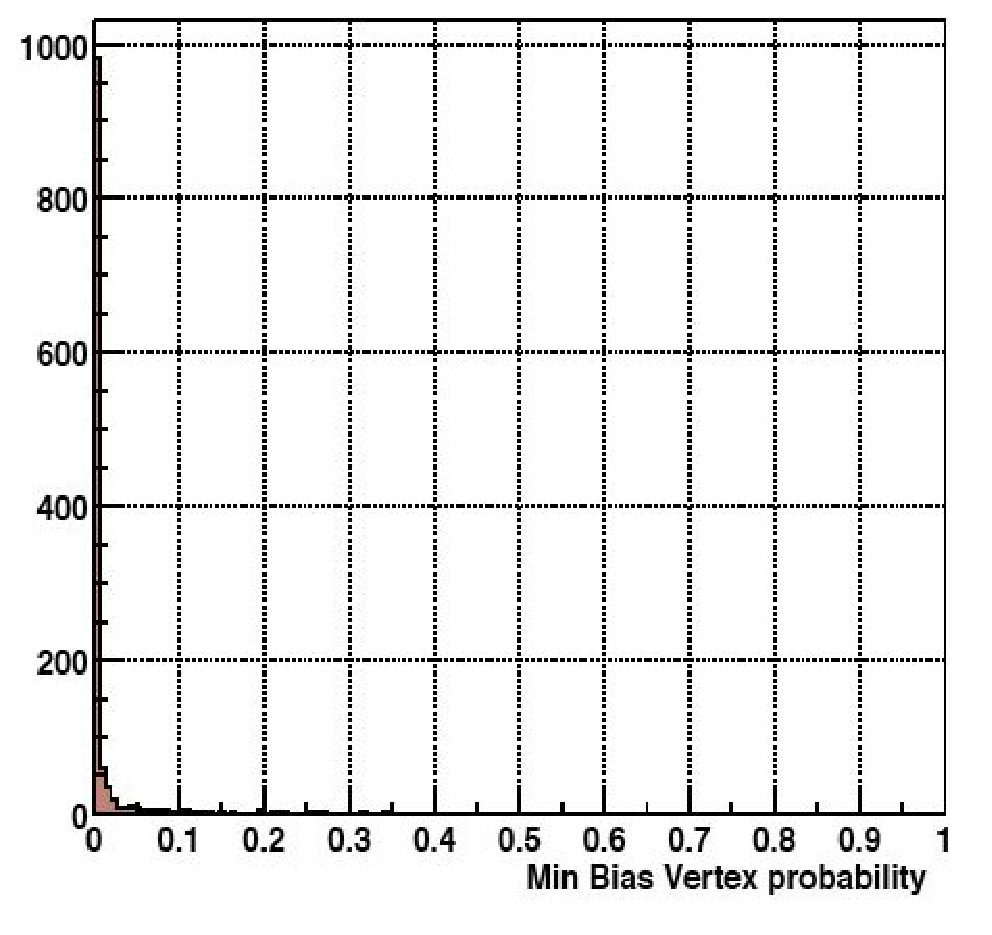
\includegraphics[width=0.49\textwidth]{eps/Reco/MBP_PV.eps}
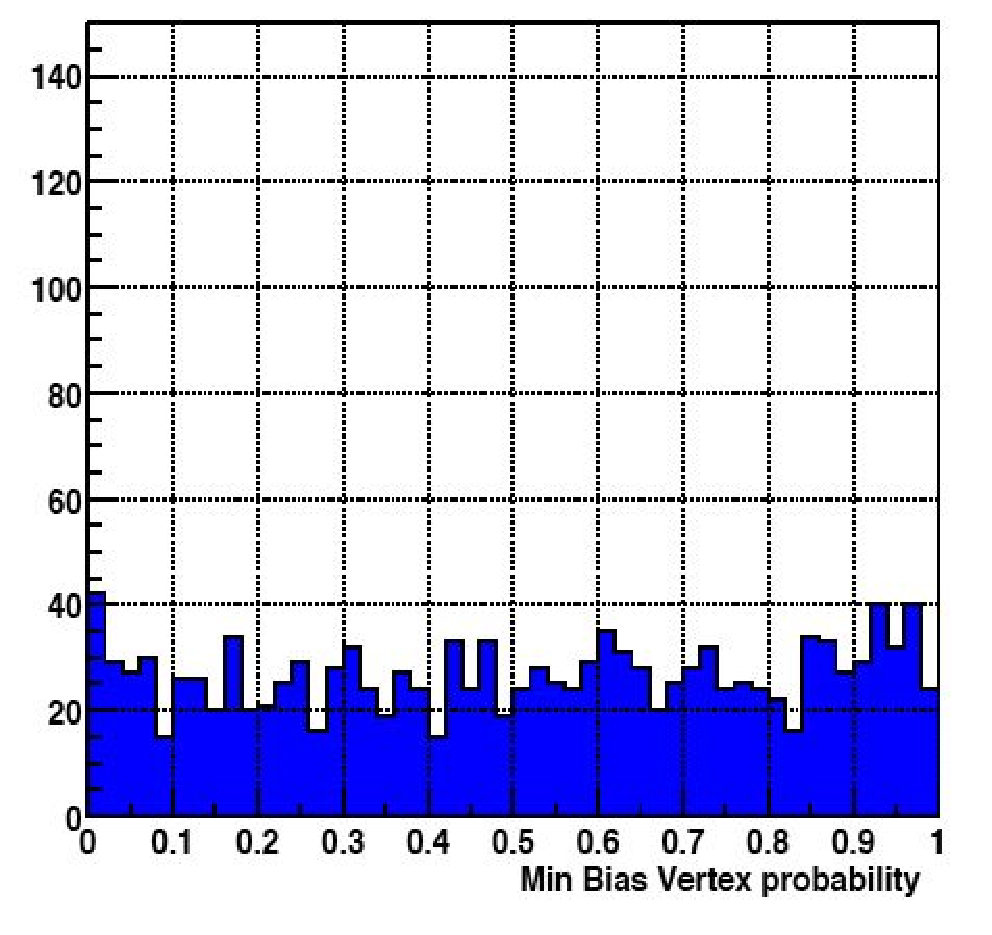
\includegraphics[width=0.49\textwidth]{eps/Reco/MBP_MB.eps}
\end{center}
\vspace{-0.1in}
\caption{Minimum bias probability for the hard scatter vertex (left) and inelastic $\ppbar$ vertices (right). The vertex in the event with the lowest minimum bias probability is selected as the hard scatter vertex~\cite{pv}.}
\label{minimum bias}
\end{figure}


\subsection{Electrons}
\label{electronreco}

Electrons in the $\dzero$~detector are characterized by narrow electromagnetic showers produced in the electromagnetic calorimeter~\cite{electron}. Initial electron candidates are first identified by a cluster of calorimeter towers in the electromagnetic calorimeter. Once a tower is found the electron candidate is defined as the towers surrounding the highest $E_{T}$ tower in a cone of radius 0.4. Since electrons will deposit most of their energy in the inner electromagnetic calorimeter the ratio of the electron candidate energy found in the electromagnetic calorimeter should be greater than $90\%$ of the energy deposited in the electromagnetic calorimeter. The shape of the electromagnetic shower should also be consistent with an electron or photon shower. Electrons are distinct from photons in that they are charged particles thus all electron candidates are required to have a track with $p_{T}>5$~GeV pointing in the direction of the electromagnetic cluster. 
To ensure that the electron is well measured it is also required to be isolated from other electromagnetic clusters. The isolation, shown in Eq.~\ref{fiso}, is defined in terms of the electromagnetic calorimeter towers with $\Delta R<0.2$ and $\Delta R<0.4$ surrounding the electron candidate and is required to be less than 0.15.

\begin{equation}
\label{fiso}
\rm{f_{iso}} = \frac{E_{EM}(\Delta R <  0.4) - E_{EM}(\Delta R <  0.2)}{E_{EM}(\Delta R <  0.4)}
\end{equation}

Finally, to ensure high quality electrons a likelihood discriminant is created using seven variables that will separate electrons from W/Z boson decays (real electrons) from jets with large electromagnetic fractions (fake electrons). Electrons with a likelihood discriminant greater than 0.85 are considered true electrons from a W/Z decay.

\subsection{Muons}
\label{muonreco}

Muon are reconstructed in the $\dzero$~detector by requiring hits in the three layers of the muon system from both the scintillators and wire chambers~\cite{muon}. A muon candidate is required to register at least two wire hits and at least one scintillator hit in the A layer.  At least two wire hits in the B and C layers as well as at least one scintillator hit in this region are also required for the muon. From the hits in the three layers it is possible to construct a local momentum measurement due to the curvature induced by the toroid magnet, however, the resolution of this measurement is quite poor. To improve the resolution, the local muon track is required to be matched with a track found by the global track reconstruction algorithm.

To remove muons produced by cosmic rays the muon candidate is required to be temporally coincident with a bunch crossing. After a bunch crossing is registered the muon candidate is required to hit all three layers within $10$~ns. To further reduce the cosmic ray background the muon track is required to originate from the primary interaction vertex with a relative longitudinal distance less than 1~cm and a transverse distance of closest approach (DCA) less than 0.2 cm if there are no SMT hits and less than 0.02 cm if there is at least one SMT hit.

Finally, an isolation cut is applied to ensure the muon is the product of a $W$ boson decay and not the result of a heavy flavor decay (e.g. $B \rightarrow \mu\nu_{\mu} D$). To remove muons from heavy flavor decays the candidate is required to be isolated ($\Delta R(\mu,\rm{jet}) > 0.5$)~from nearby jets since muons from heavy flavor decays will tend to be found inside or near a jet. To further reject muons from heavy flavor decays, two isolation variables are defined in terms of the muon track $p_{T}$ and the sum of either calorimeter energy or track momentum surrounding the muon momentum vector. The two isolation variables, shown in Eq.~\ref{trackiso} and~\ref{caliso}~are both required to be less than 0.2.

\begin{equation}
\label{trackiso}
f_{\rm{Track~Isolation}}(\mu, \rm{Tracks}) = \frac{1}{p_{T}(\mu)} \times \sum_{\rm{tracks \neq muon~ \Delta R < 0.5 }}p_{T}(\rm{track})
\end{equation}

\begin{equation}
\label{caliso}
f_{\rm{Calorimeter~Isolation}}(\mu, \rm{CalTowers}) = \frac{1}{p_{T}(\mu)} \times \sum_{\rm{cal~tower~0.1 < \Delta R < 0.4 }}E_{T}(\rm{cal~tower})
\end{equation}
%  author = {J. Hays, J. Mitrevski, C. Schwanenberger, T. Toole},


\subsection{Jets}
\label{jetreco}

A jet is defined as a narrow cone of strongly interacting particles produced by the hadronization of strongly interacting particles such as quarks or gluons. A jet will shower in the electromagnetic and hadronic calorimeters and its energy is measured by sampling this shower in the many layers of the $\dzero$~calorimeter. A proper measurement of the jet energy and direction is needed to determine the original quark or gluon energy and momentum.

The Run II improved legacy cone algorithm~\cite{Blazey:2000qt} is used to reconstruct jets in the $\dzero$ calorimeter. This algorithm selects calorimeter towers with transverse energies\footnote{The transverse energy is the energy of the calorimeter tower weighted by the sine of the polar angle $\theta$ of the tower (i.e. $E_{T} = E \times \sin(\theta)$).} greater than $0.5$~GeV as seeds around which the jet is built. The algorithm collects all calorimeter towers in a cone\footnote{The jet cone is defined in terms of rapidity ($y$) and azimuthal angle ($\phi$).} of radius $0.5$ around the seed tower and defines this as the jet candidate if it has $E_{T}>1$~GeV. The central axis of the jet is defined by the $E_{T}$ weighted midpoints of each calorimeter tower. This procedure is repeated throughout the detector until all jets are stable (i.e. the jet axis from one iteration to the next does not change) with a total $E_{T}>6$~GeV. The final step of the jet finding algorithm is to remove overlapping jets. A jet is defined as overlapping if it shares energy with another jet. Two overlapping jets are merged if the overlapping energy is more than half of the individual jet energies. If the overlapping jets are not merged, then they are split into two distinct jets whose total $E_{T}$ and axis are recomputed.

%Cone jets have several advantages both experimentally and theoretically. Since the jets are defined by rapidity and $\phi$, they are invariant under boosts along the longitudinal direction (beam axis). This is important because the longitudinal boost of events at the Tevatron will typically be large with resepect to the $\ppbar$~rest frame. The other advantage of cone jets is they are infrared safe meaning that one can calculate jet properties in the low energy regime of a theory without incurring singularities.

Once the jets have been reconstructed a set of quality criteria are applied to remove fake jets created out of calorimeter noise and remove electromagnetic particles such as electrons and photons. To remove jets created by electromagnetic particles a jet is required to have between 5 and 95$\%$ of its energy deposited in the hadronic calorimeter. Also, a jet is required to be isolated ($\Delta R>0.5$) from all electromagnetic clusters in the detector. To remove fake jets created by calorimeter noise the jet is required to have at least 60$\%$ of its energy deposited in the fine hadronic calorimeter since this detector has higher energy resolution than the coarse hadronic calorimeter. Jets created by a single ``noisy" cell are removed by requiring that more than one calorimeter cell contain at least $90\%$ of the jet energy. Also, to further suppress the effect of a noisy cell the ratio of the most energetic tower to the second most energetic tower must be less than 10.

\subsubsection{Jet Energy Scale Correction}

In reconstructing physics objects in an event, the goal is to measure the four-momenta of the final state particles from the hard scatter collision. For jets this is quite complicated due to the nearly 4 radiation lengths of material that separate the collision center from the calorimeter. It is the goal of the jet energy scale correction to modify the calorimeter jet energies to the parton energy before any interaction with the $\dzero$~detector~\cite{jes}.

The corrected jet energy, which is defined as the energy of a final state parton before interacting with the detector, is given by Eq.~\ref{jes} in terms of five other quantities, which are explained below.

\begin{equation}
\label{jes}
E_{\rm{jet}}^{\rm{corr}} = \frac{E_{\rm{jet}}^{\rm{uncorr}} - \rm{O}}{\rm{F}_{\eta} \times \rm{R} \times \rm{S}}
\end{equation}

\begin{itemize}
\item $E_{\rm{jet}}^{\rm{uncorr}}$ is the uncorrected jet energy as determined by the reconstruction algorithm.

\item O is the offset correction and represents energy that contributes to the jet that is not associated with the hard scatter collision. Two examples of additional sources of energy are electronics noise and additional minimum bias interactions in the same bunch crossing. The offset correction is measured in minimum bias events by summing the energy of calorimeter towers within a jet cone radius. A plot of the offset energy correction as a function of the detector pseudorapidity ($\eta^{\rm{det}}$)\footnote{$\eta^{\rm{det}}$ is the pseudorapidity defined with respect to the detector origin instead of the collision center.} for several primary vertex multiplicities is shown in Fig.~\ref{jesoffset}.

\begin{figure}[!h!tbp]
\begin{center}
\includegraphics[width=0.75\textwidth]{eps/Reco/jes-offset.eps}
\end{center}
\vspace{-0.1in}
\caption{Offset energy correction for jets with a cone radius of 0.5 as a function of $\eta^{det}$~\cite{jes}.}
\label{jesoffset}
\end{figure}

\item F$_{\eta}$ is the relative response of the calorimeter in different $\eta$~regions. This term is designed to cancel the expected non-uniformity of the $\dzero$~calorimeter between the central and endcap  calorimeter cryostats. The relative response is measured using the missing $E_{T}$ projection fraction method in back-to-back one photon with one jet events. In this method the photon is considered perfectly well measured, which implies that that any E$_{T}$ imbalance in the event is an effect of the response. A cartoon of the method is shown in Fig.~\ref{metprojection}.

\begin{figure}[!h!tbp]
\begin{center}
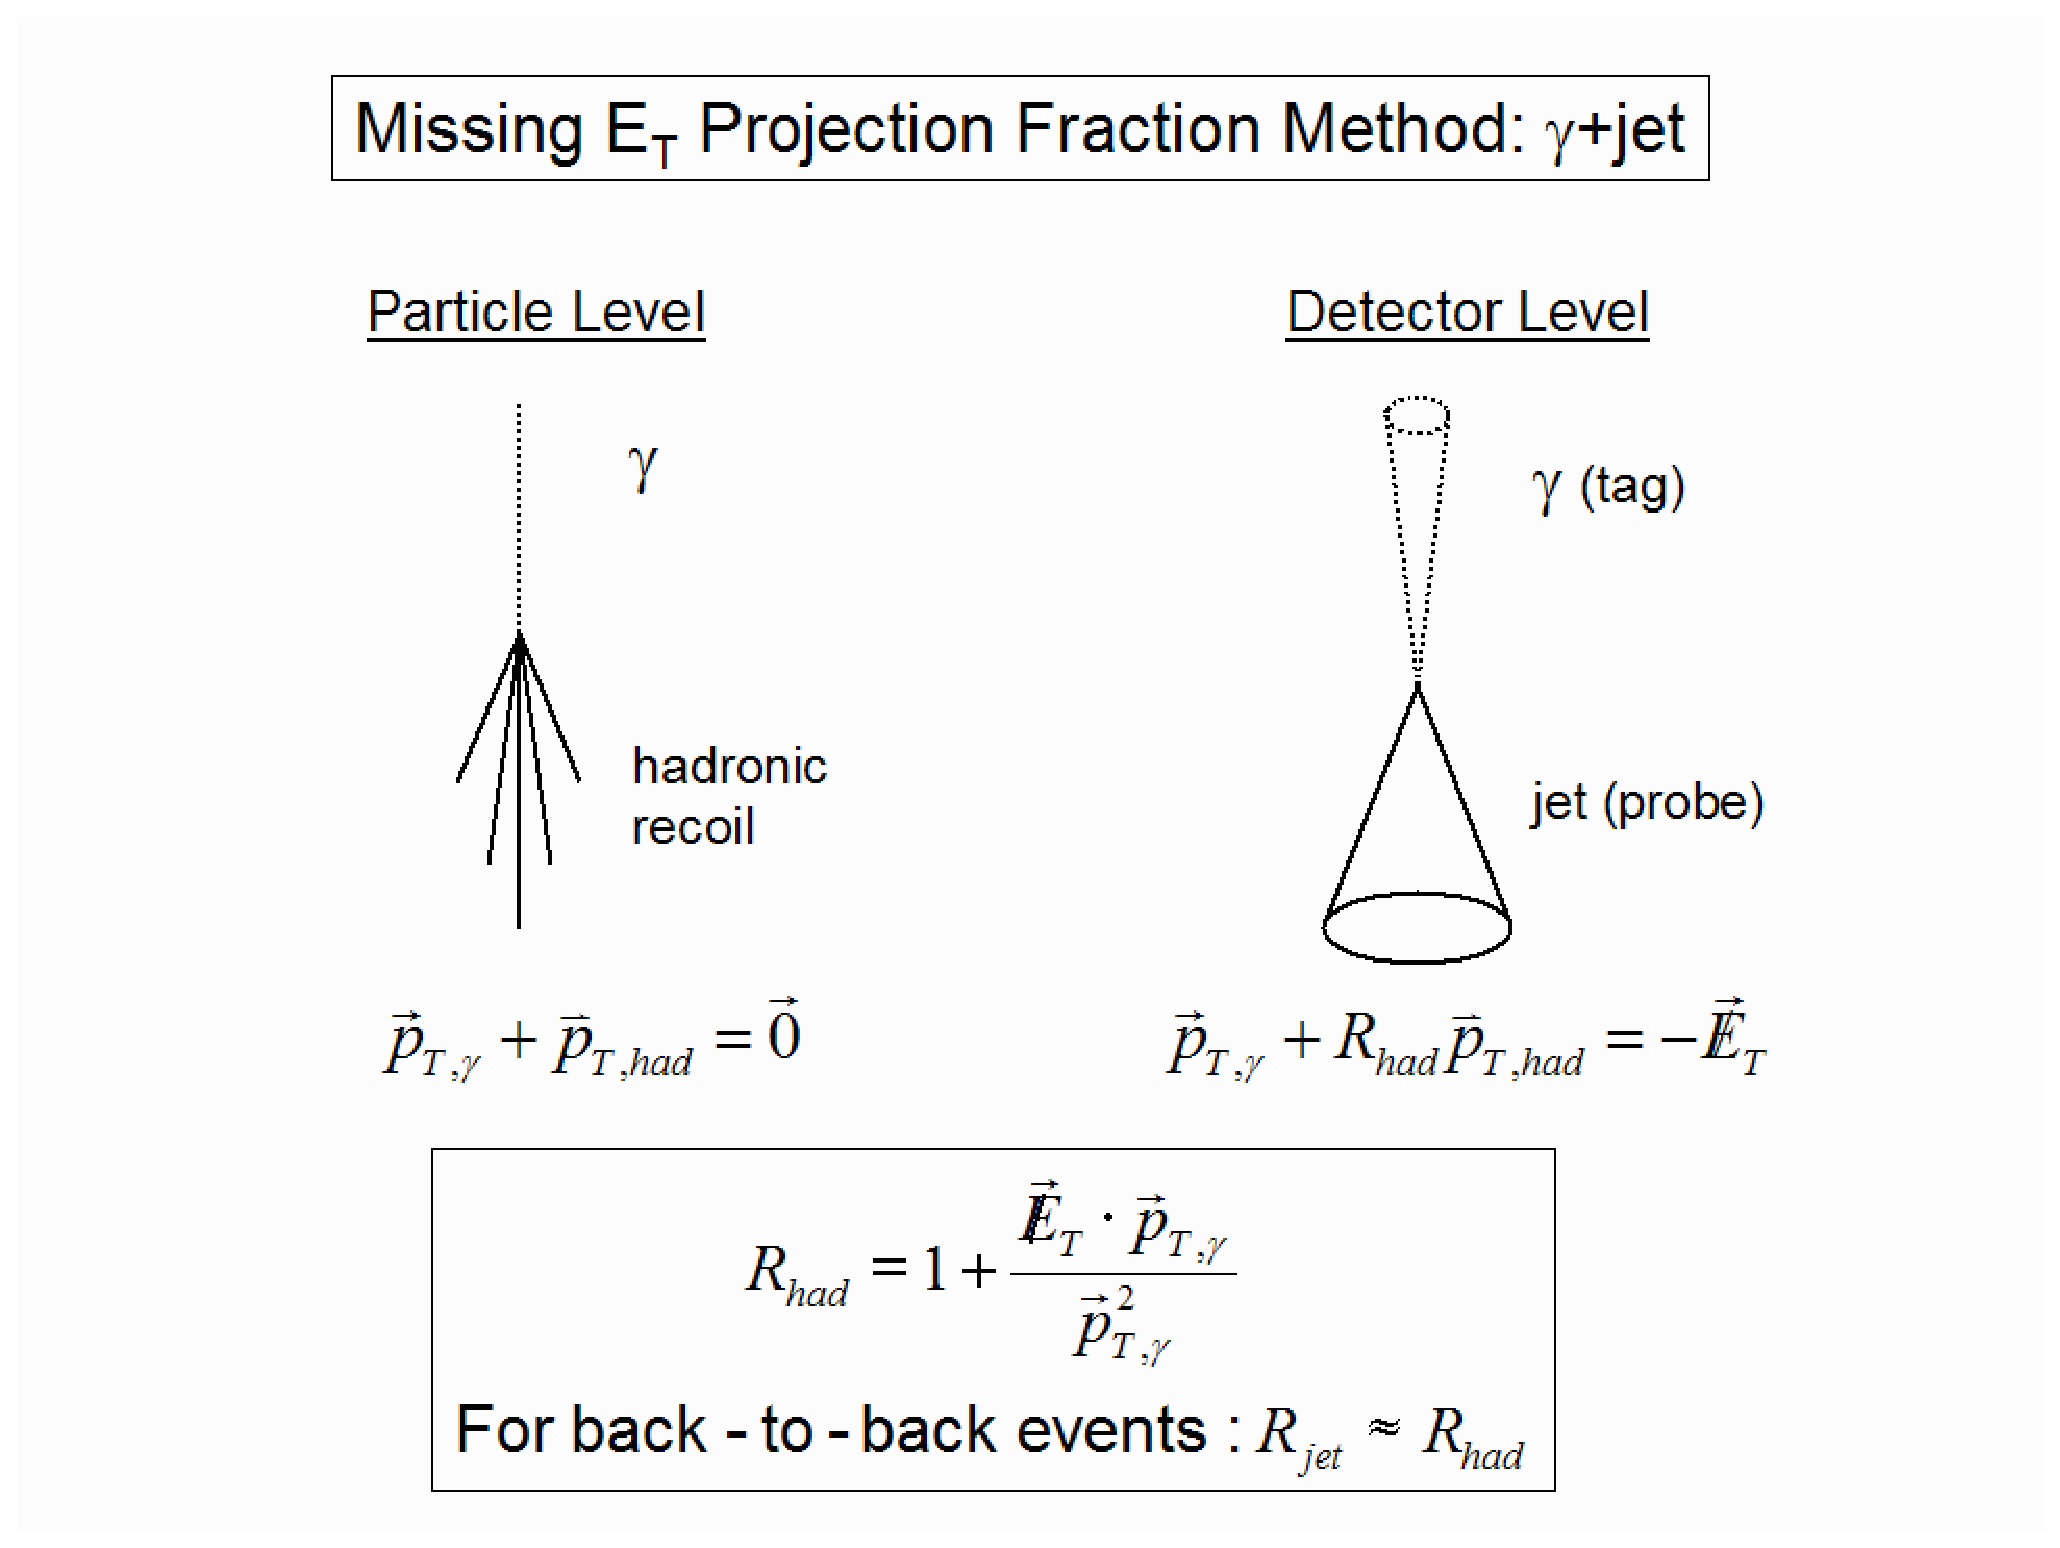
\includegraphics[width=0.75\textwidth]{eps/Reco/JES-relative-method.eps}
\end{center}
\vspace{-0.1in}
\caption{Missing $E_{T}$ ($E_{T}$ imbalance) projection fraction method cartoon~\cite{jes}.}
\label{metprojection}
\end{figure}

By measuring the missing E$_{T}$ and the $p_{T}$ of the photon and jet the response relative to $\eta=0$ can be measured in many regions of $\eta^{\rm{det}}$. The relative response with respect to $\eta=0$~in data is shown in Fig.~\ref{jes-relative}.

\begin{figure}[!h!tbp]
\begin{center}
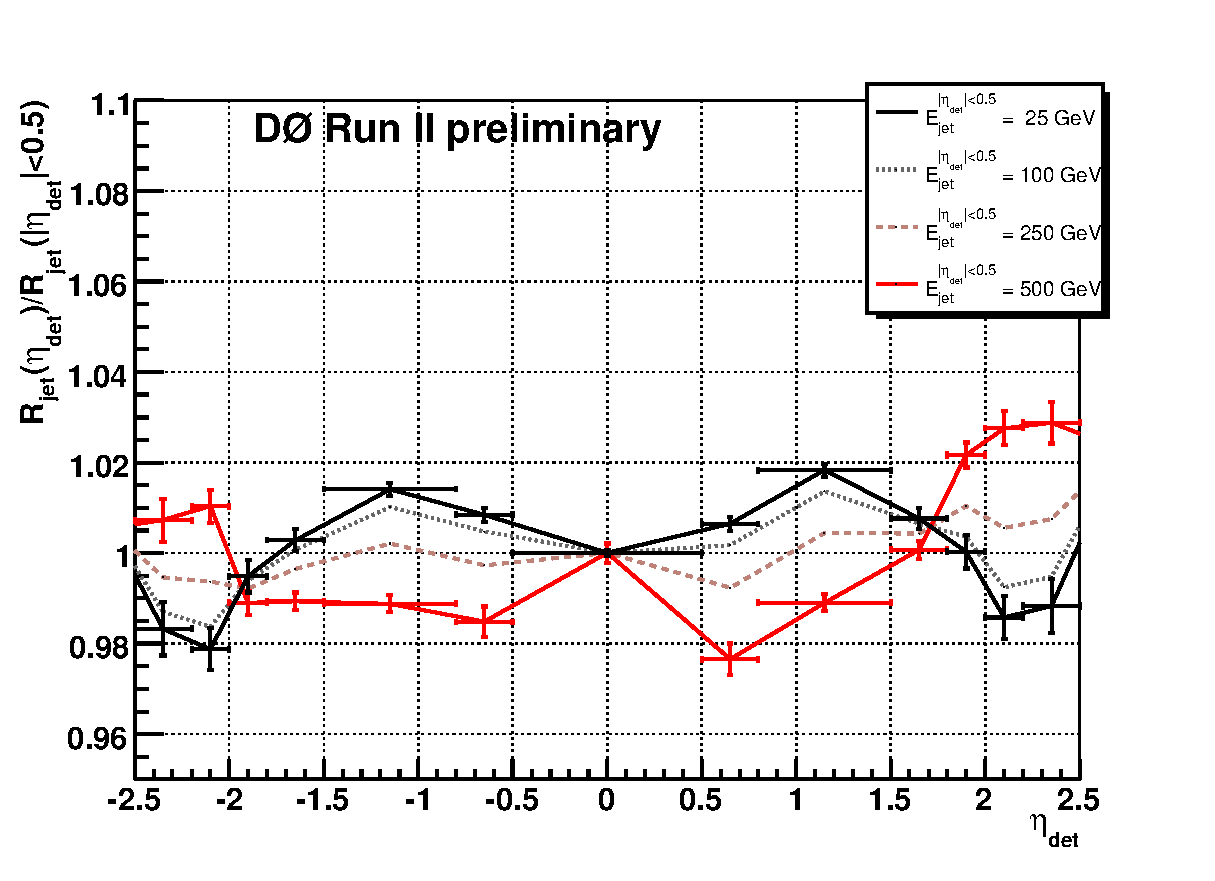
\includegraphics[width=0.75\textwidth]{eps/Reco/JES-relative.eps}
\end{center}
\vspace{-0.1in}
\caption{The relative energy correction for jets with a cone radius of 0.5 as a function of $\eta^{det}$ (right)~\cite{jes}.}
\label{jes-relative}
\end{figure}
 
\item R is the absolute energy response of the calorimeter. This term accounts for energy lost in un-instrumented regions of the detector and the lower energy response of the calorimeter to hadrons compared to electrons or photons. The absolute response is also determined using back-to-back photon+jet events and is measured after the relative response in $\eta$ has been applied. Fig.~\ref{jes-absolute} shows the absolute energy response for different $\eta$ regions to emphasize the uniformity of the calorimeter after applying the relative response term.

\begin{figure}[!h!tbp]
\begin{center}
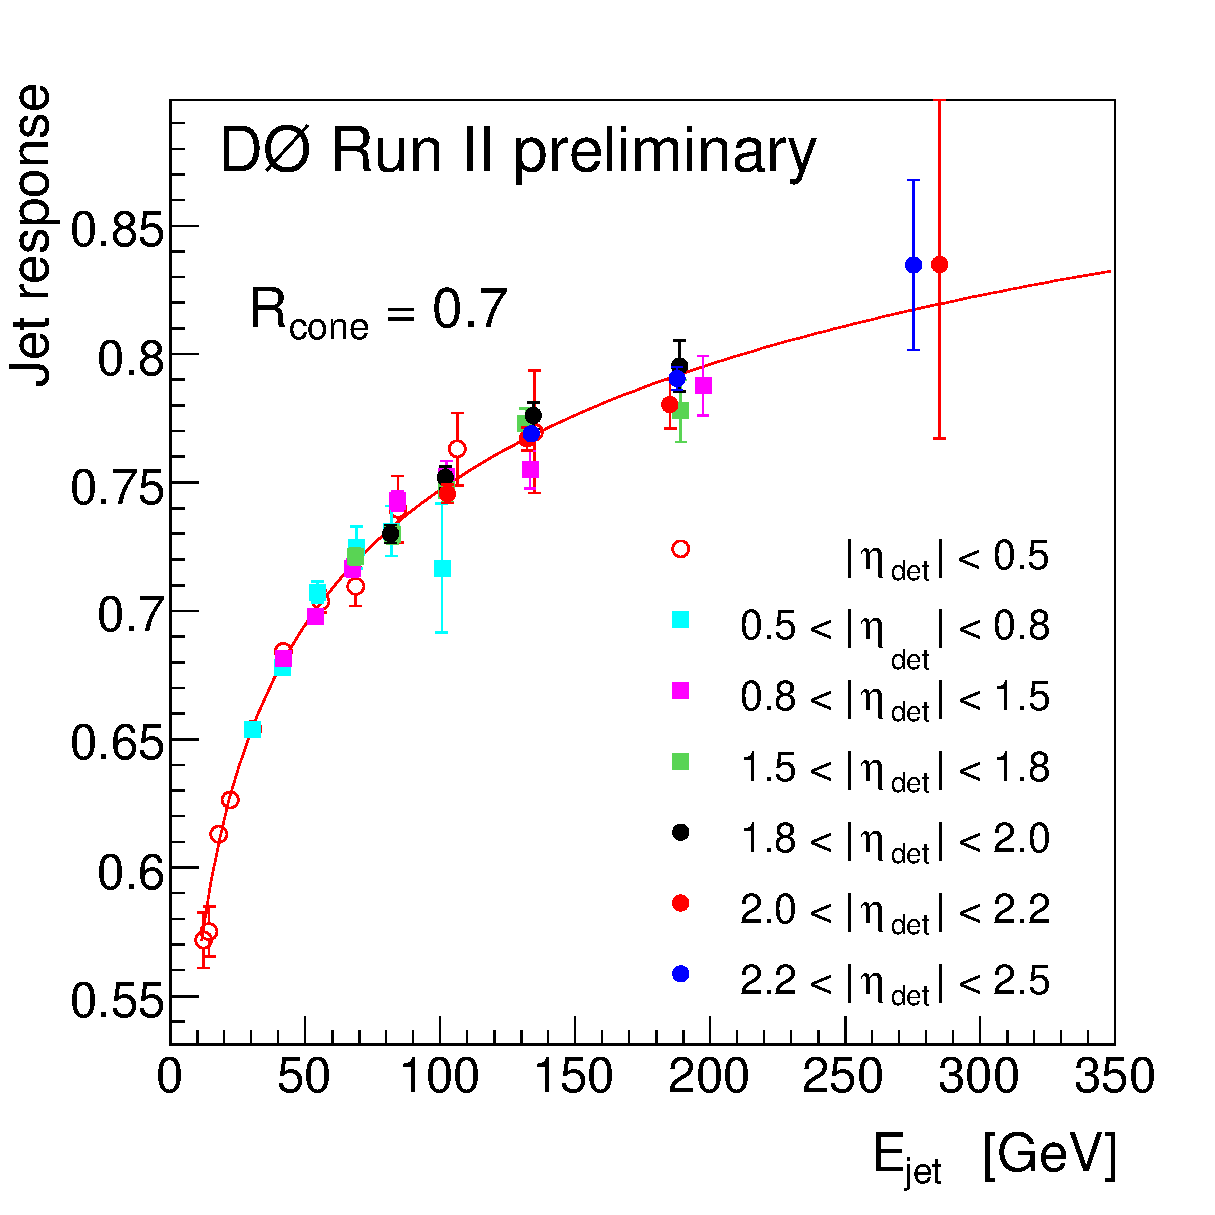
\includegraphics[width=0.75\textwidth]{eps/Reco/JES-absolute.eps}
\end{center}
\vspace{-0.1in}
\caption{Absolute energy response of jets in the calorimeter for several $\eta$ regions~\cite{jes}.}
\label{jes-absolute}
\end{figure}

\item S is the showering correction. This term corrects for energy deposited outside the cone radius of the reconstructed jet or additional energy deposited inside the cone radius as a result of spurious particles in the calorimeter. The showering correction is measured by calculating the total energy deposited inside and outside the jet and taking the ratio of these numbers with the known deposited energy as determined in Monte Carlo events. The calculation in Monte Carlo is done without detector simulation such that the ratio of the two quantities yields the showering correction due to the detector only. Fig.~\ref{jes-shower} shows the showering correction as a function of jet E$_{T}$ for jets in three different $\eta$ regions.

\begin{figure}[!h!tbp]
\begin{center}
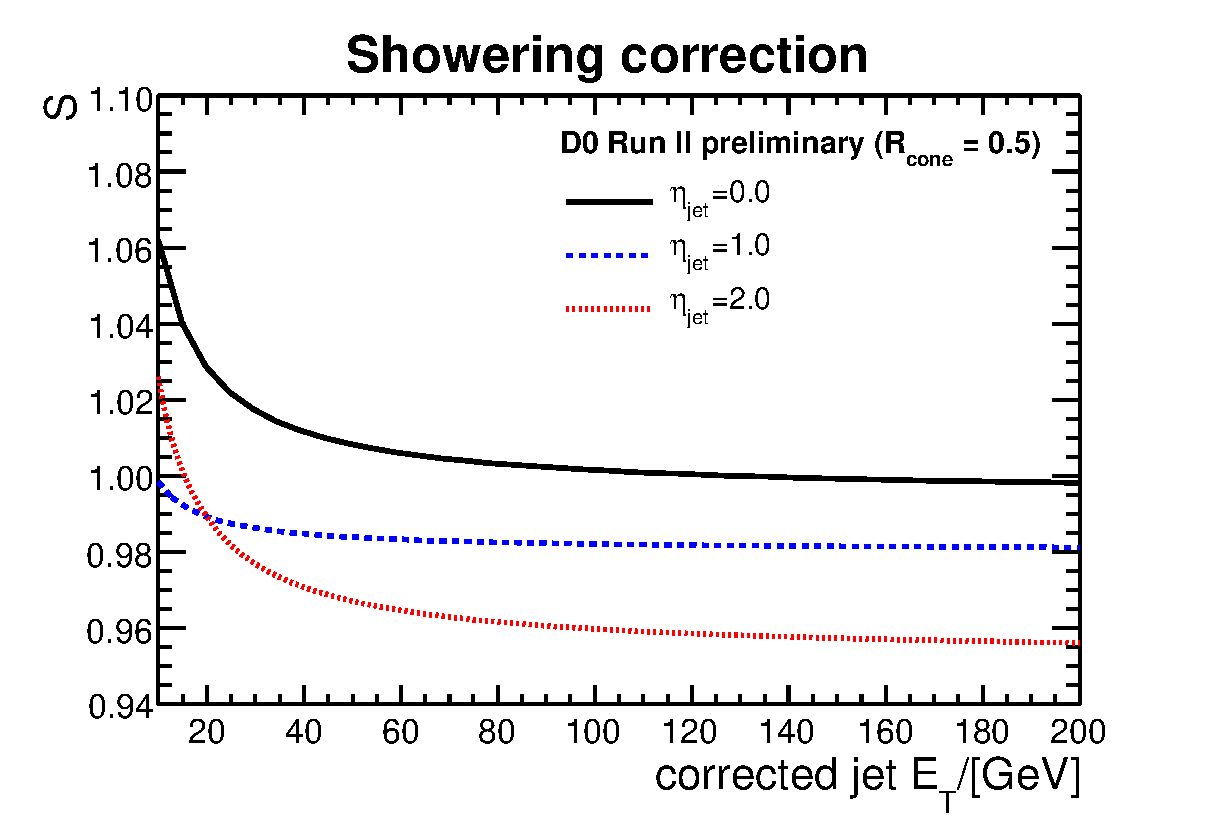
\includegraphics[width=0.75\textwidth]{eps/Reco/JES-shower.eps}
\end{center}
\vspace{-0.1in}
\caption{Showering correction for jets as a function of E$_{T}$ for jets in three different $\eta$ regions~\cite{jes}.}
\label{jes-shower}
\end{figure}

\end{itemize}

\subsection{Missing $E_{T}$}
\label{metreco}

Missing transverse energy is a useful quantity to calculate because it is highly correlated with the transverse energy of the undetected neutrino. The missing energy is only calculated in the transverse plane (x-y) because there is no net momentum in this plane since the proton-antiproton collision only occurs along the beam axis (z)\footnote{The total missing energy of the event can not be calculated because of the unknown boost along the longitudinal direction from the hard scatter process.}.  The missing $E_{T}$ (M$E_{T}$) is defined as the vector sum of the electromagnetic and fine hadronic calorimeter cell energies as well as any lepton $p_{T}$ subtracted from zero such that there is no net transverse momentum in the event. This definition is summarized in Eq.~\ref{met}.

\begin{equation}
\label{met}
\rm{M}E_{T} = -\left[~\sum_{\rm{cells}} E_{T}~\right] - p_{T}(\ell)
\end{equation}

\subsection{$B$-Jets}
\label{bidreco}

$B$-jets are a subset of all jets found by the jet cone algorithm with the distinction that these jets are formed from the hadronization of a $b$ quark. $B$-jets are important to measure because many fundamental particles, such as the top quark, will decay into a $b$ quark leaving it as one of the few signatures of its existence. $B$-jets are unique from jets produced from light quarks because the $B$~hadron (a bound state of a $b$ quark and one or two light quarks) has a much longer lifetime than lighter hadrons. The result of this long lifetime is a displaced decay vertex from the primary interaction vertex. The typical decay length, which is the distance from the decay vertex to the primary vertex, is a few millimeters. The goal of a $B$-jet finding algorithm is to use this property and other kinematically unique characteristics to identify heavy flavor jets from light flavor jets.

The $B$-jet selection algorithm at $\dzero$~uses a neural network (NN) to distinguish heavy flavor jets from light flavor jets~\cite{bid}. The neural network is trained using seven variables that show discrimination between heavy and light flavor jets. The seven variables are shown in Table~\ref{nnvars}.  The network was trained with $Z\rightarrow b\bar{b}$ and strongly produced $b\bar{b}$ production as heavy flavor signal-like events and $Z\rightarrow q\bar{q}$ and strongly produced $q\bar{q}$ production as light flavor background-like events. The output of the neural network is a new variable which peaks at 1 for heavy flavor jets and 0 for light flavor jets. A jet is ``tagged" as a $B$-jet if the NN value is greater than 0.775. Only jets with at least two tracks with $p_{T}>1$~GeV are considered for heavy flavor tagging. Jets which fail this criteria are considered light flavor jets.

\begin{table}[!h!tbp]
\begin{center}
\caption{Variables used in the neural networks training. The variables are listed in order of relative importance as determined in the training~\cite{bid}.}
\label{nnvars}
\begin{tabular}{c|c}
%\multicolumn{2}{c}
%{\underline{Variables Used in $B$-jet Neural Network}} \\
Rank	&	Variable Description	\\
\hline
1		&	Decay length significance ($\frac{L_{T}}{\delta L_{T}}$) of the displaced vertex	\\
2		&	Weighed combination of the input tracks' impact parameter significance ($\frac{IP}{\delta IP}$)	\\
3		&	Probability that the jet originates from the primary interaction vertex	\\
4		&	$\chi^{2}$/N$_{dof}$ of the displaced vertex fit	\\
5		&	Number of tracks used to reconstruct the displaced vertex	\\
6		&	Mass of the tracks used to reconstruct the displaced vertex	\\
7		&	Number of displaced vertices found inside the input jets		\\
\end{tabular}
\vspace{-0.1 in}
\end{center}
\end{table} 

%------------------------------------


\section{Monte Carlo Generation and Detector Simulation}
\label{simulation}

Generating Monte Carlo events is crucial in a physics analysis to understand the signature a given process will have in the detector. The chain for generating simulated Monte Carlo events at $\dzero$ is the following: (1) generate final state four-vectors using Monte Carlo software, (2) simulate the $\dzero$~detector response to final state particles, (3) add additional $\ppbar$~interactions, and finally (4) reconstruct the event. The $\dzero$~trigger simulation is performed separately and described in Section~\ref{triggersim}. The result of the Monte Carlo generation with full detector simulation is a set of events that can be treated as equal to reconstructed data except with a known initial hard scatter physics process.

The first stage of generating Monte Carlo events is to produce and decay particles according to a specified physics process. The hard scatter collision is typically generated by ``matrix-element" generators, such as CompHEP or Alpgen, and the decay products are typically handled by particle-specific algorithms. Specifically, the decay of tau leptons is handled by TAUOLA~\cite{1993CoPhC..76..361J} and B hadrons are decayed by EVTGEN~\cite{2001NIMPA.462..152L}. To simulate hardronization and allow for additional strong interaction effects between final state particles, all Monte Carlo events are processed through the Pythia generator.

The $\dzero$~detector is simulated using the GEANT software package~\cite{geant}. GEANT\footnote{GEANT is an acronym formed from "GEometry ANd Tracking".} provides a graphical representation of particles as they traverse the detector and simulates the interaction between particles and material in the detector. All information concerning the detector geometry and material density is modeled with GEANT. Three examples of GEANT's capabilities are simulating electromagnetic and hadronic showers in the calorimeter, energy loss of electrons in the tracking detector, and bending particle trajectories due to the solenoidal and toroidal magnetic fields.

To properly account for additional inelastic $\ppbar$~collisions all Monte Carlo events are provided with a ``minimum bias overlay" generated from reconstructed data. A minimum bias event is an event recorded by the detector that was triggered solely by the presence of at least one $\ppbar$~interaction. Because the number of minimum bias vertices grows with instantaneous luminosity the minimum bias events are overlaid to match the expected instantaneous luminosity profile of all recorded events. A plot of the average peak instantaneous luminosity versus time is shown in Fig.~\ref{peaklumi}.

\begin{figure}[!h!tbp]
\begin{center}
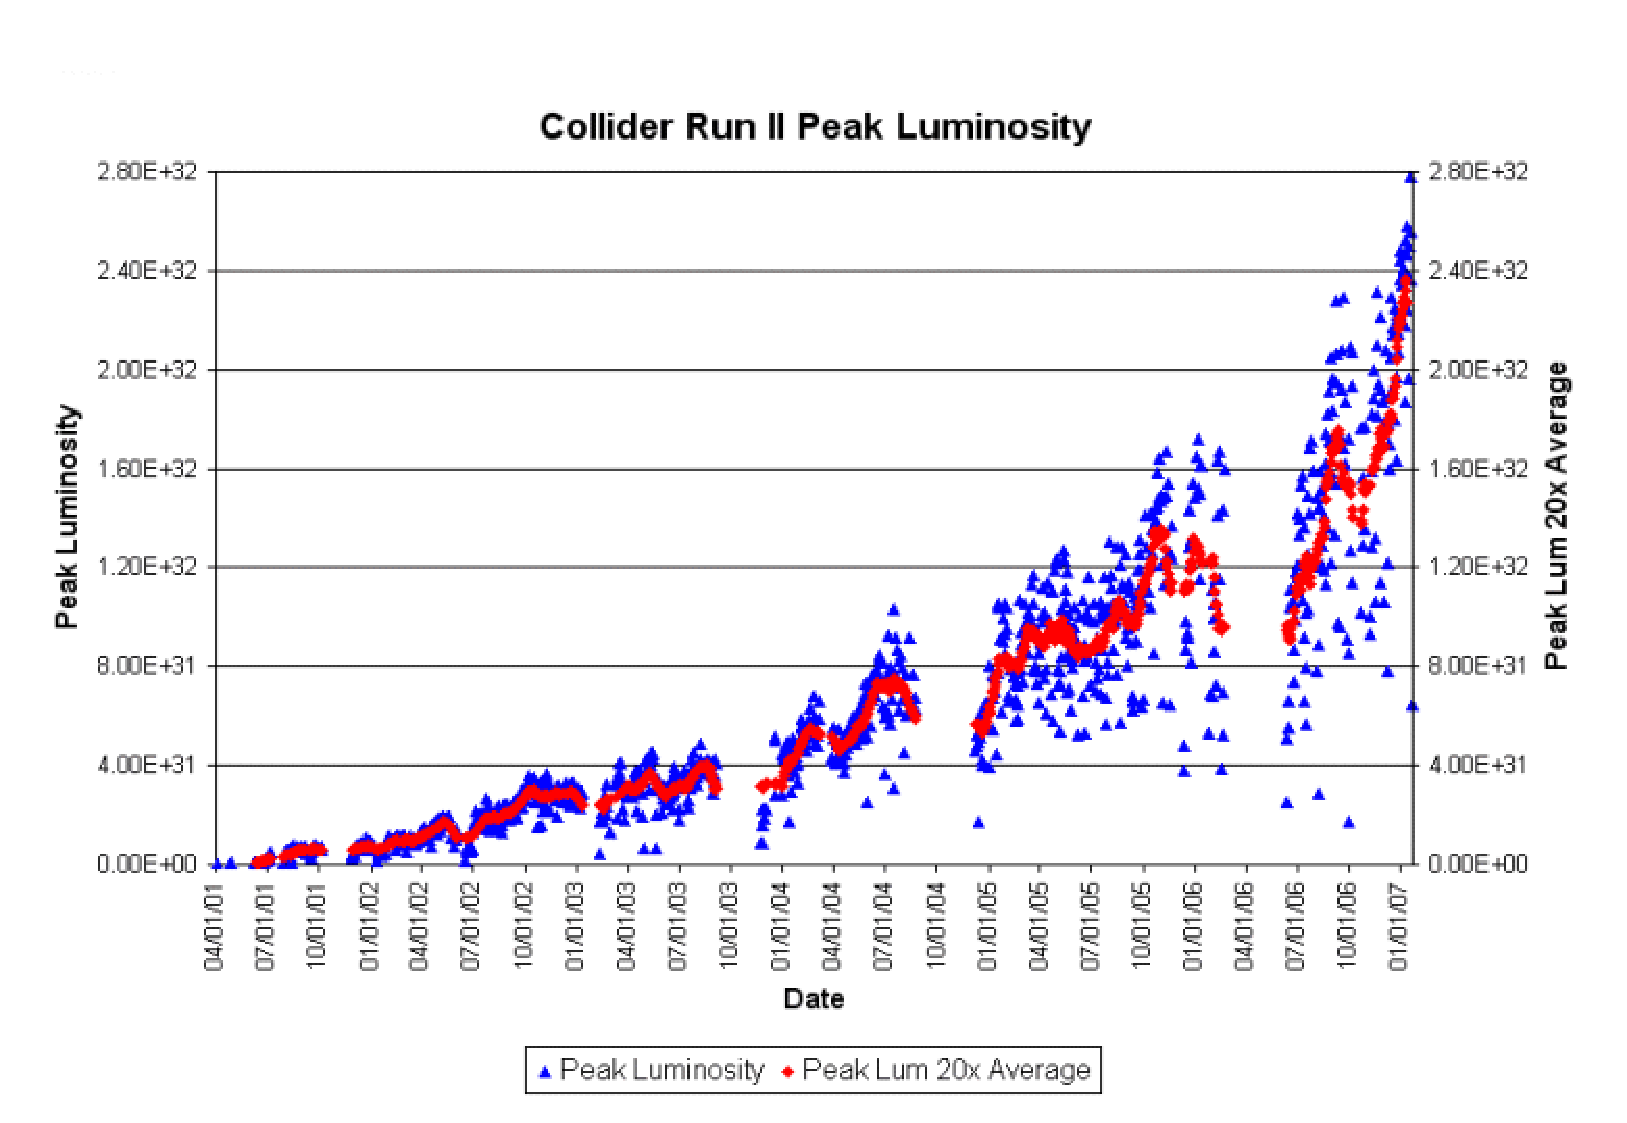
\includegraphics[width=0.75\textwidth]{eps/Reco/InstanteousLuminosity.eps}
\end{center}
\vspace{-0.1in}
\caption{Peak instantaneous luminosity as a function of time~\cite{tevlumi}.}
\label{peaklumi}
\end{figure}

Reconstruction of Monte Carlo events occurs in the same manner as data events, as described in Section~\ref{objectreco}. It is the goal of the previous three steps of the simulation chain to describe the $\dzero$~detector response as accurately as possible such that the reconstruction is blind to the source of the event.

\section{Trigger Simulation}
\label{triggersim}

The $\dzero$~trigger system is modeled in a Monte Carlo event by an event-wide probability that the event will pass the trigger selection. The event-wide probability is constructed from the efficiencies with which individual reconstructed objects pass object specific ``trigger terms". Section~\ref{triggerprob} derives the event-wide trigger probability in terms of individual trigger term efficiencies and Section~\ref{triggereffmethod} describes the methods used to measure these efficiencies. Triggers used to record single top quark events and their efficiencies are shown in Chapter~\ref{analysis}.

\subsection{Event-Wide Trigger Probability}
\label{triggerprob}

The probability that a Monte Carlo event $\vec{x}$ is selected by the trigger is defined as a product of the condition probabilities to pass each trigger level given that it passed the previous trigger level as shown in Eq.~\ref{trigprob}.

\begin{equation}
\label{trigprob}
P_{\rm{Trigger}}(\vec{x}) = \left[ \prod_{\rm{Terms}}P_{\rm{L1}}(\vec{x}) \right ] \times \left[ \prod_{\rm{Terms}}P_{\rm{L2|L1}}(\vec{x}) \right ] \times \left[ \prod_{\rm{Terms}}P_{\rm{L3|L2}}(\vec{x}) \right ]
\end{equation}

At a given trigger level the probability for the event to be selected is written as the product of each reconstructed object to be selected by each trigger term as shown in Eq.~\ref{triglevelprob}. For example, the probability for a muon+2~jet event to pass a $\mu$+jets trigger is the product of the probability for the muon to pass the muon trigger term and the two jets to pass the jet trigger term.

\begin{equation}
\label{triglevelprob}
P_{\rm{Level}}(\vec{x}) = \prod_{k}^{\rm{Nobs}} P_{\rm{Level,Object}}(\vec{x}_{\rm{Object}})
\end{equation}

The probability for a reconstructed object to pass a certain trigger level is written as one minus the probability of all the objects not to be selected by the trigger, as shown in Eq.~\ref{triglevelprobobject}

\begin{equation}
\label{triglevelprobobject}
P_{\rm{Level,Object}}(\vec{x}_{\rm{Object}}) = 1 - \prod_{j}^{\rm{Nobjs}}( 1 - \varepsilon_{\rm{Level}}(\vec{x}_{\rm{Object},j}) )
\end{equation}

\noindent where $\varepsilon_{\rm{Level}}(\vec{x}_{\rm{Object},j})$~is the trigger term efficiency for the reconstructed object.

At $\dzero$ there have been several distinct trigger periods where the trigger used to collect data events has changed. To model this in Monte Carlo an integrated luminosity weighted average of the trigger probabilities for each period is applied to all events. The weighted averaged is shown in Eq.~\ref{triggerweight}

\begin{equation}
\label{triggerweight}
P(\vec{x}) = \frac{\sum_{\rm{version}} \left[ \mathcal{L}_{\rm{version}} \times P_{\rm{version}}(\vec{x}) \right]}{\sum_{\rm{version}} \mathcal{L}_{\rm{version}}}
\end{equation}

\subsection{Trigger Term Efficiency Measurement Methods}
\label{triggereffmethod}

Electron and muon trigger term efficiencies are measured in $Z\rightarrow ee$ and $Z\rightarrow \mu\mu$ data events, respectively. The efficiency is measured in a $Z$ boson sample because it provides a clean (i.e. negligible background) sample of leptons with which to measure efficiencies. In the $Z$ sample a ``tag and probe" method is used to measure the trigger efficiency where one of the leptons is required to trigger the event such that the other can be used as an unbiased probe to measure the trigger efficiency. The efficiency is defined as the fraction of events for which the probe electron or muon was found to pass the trigger term. To account for detector and reconstruction effects the trigger efficiencies are determined as a function of $p_{T}$, $\eta$, or $\phi$. An example of the L1 muon trigger efficiency and the L3 electron trigger efficiency binned in $\eta$ and $p_{T}$ are shown in Fig.~\ref{triggereffexample}. Jet trigger term efficiencies are measured in muon triggered events. The jet trigger efficiency is defined as the number of jets that pass the jet trigger term divided by the total number of jets. Jet trigger term efficiencies are measured as a function of $p_{T}$ and $\eta$.


\begin{figure}[!h!tbp]
\begin{center}
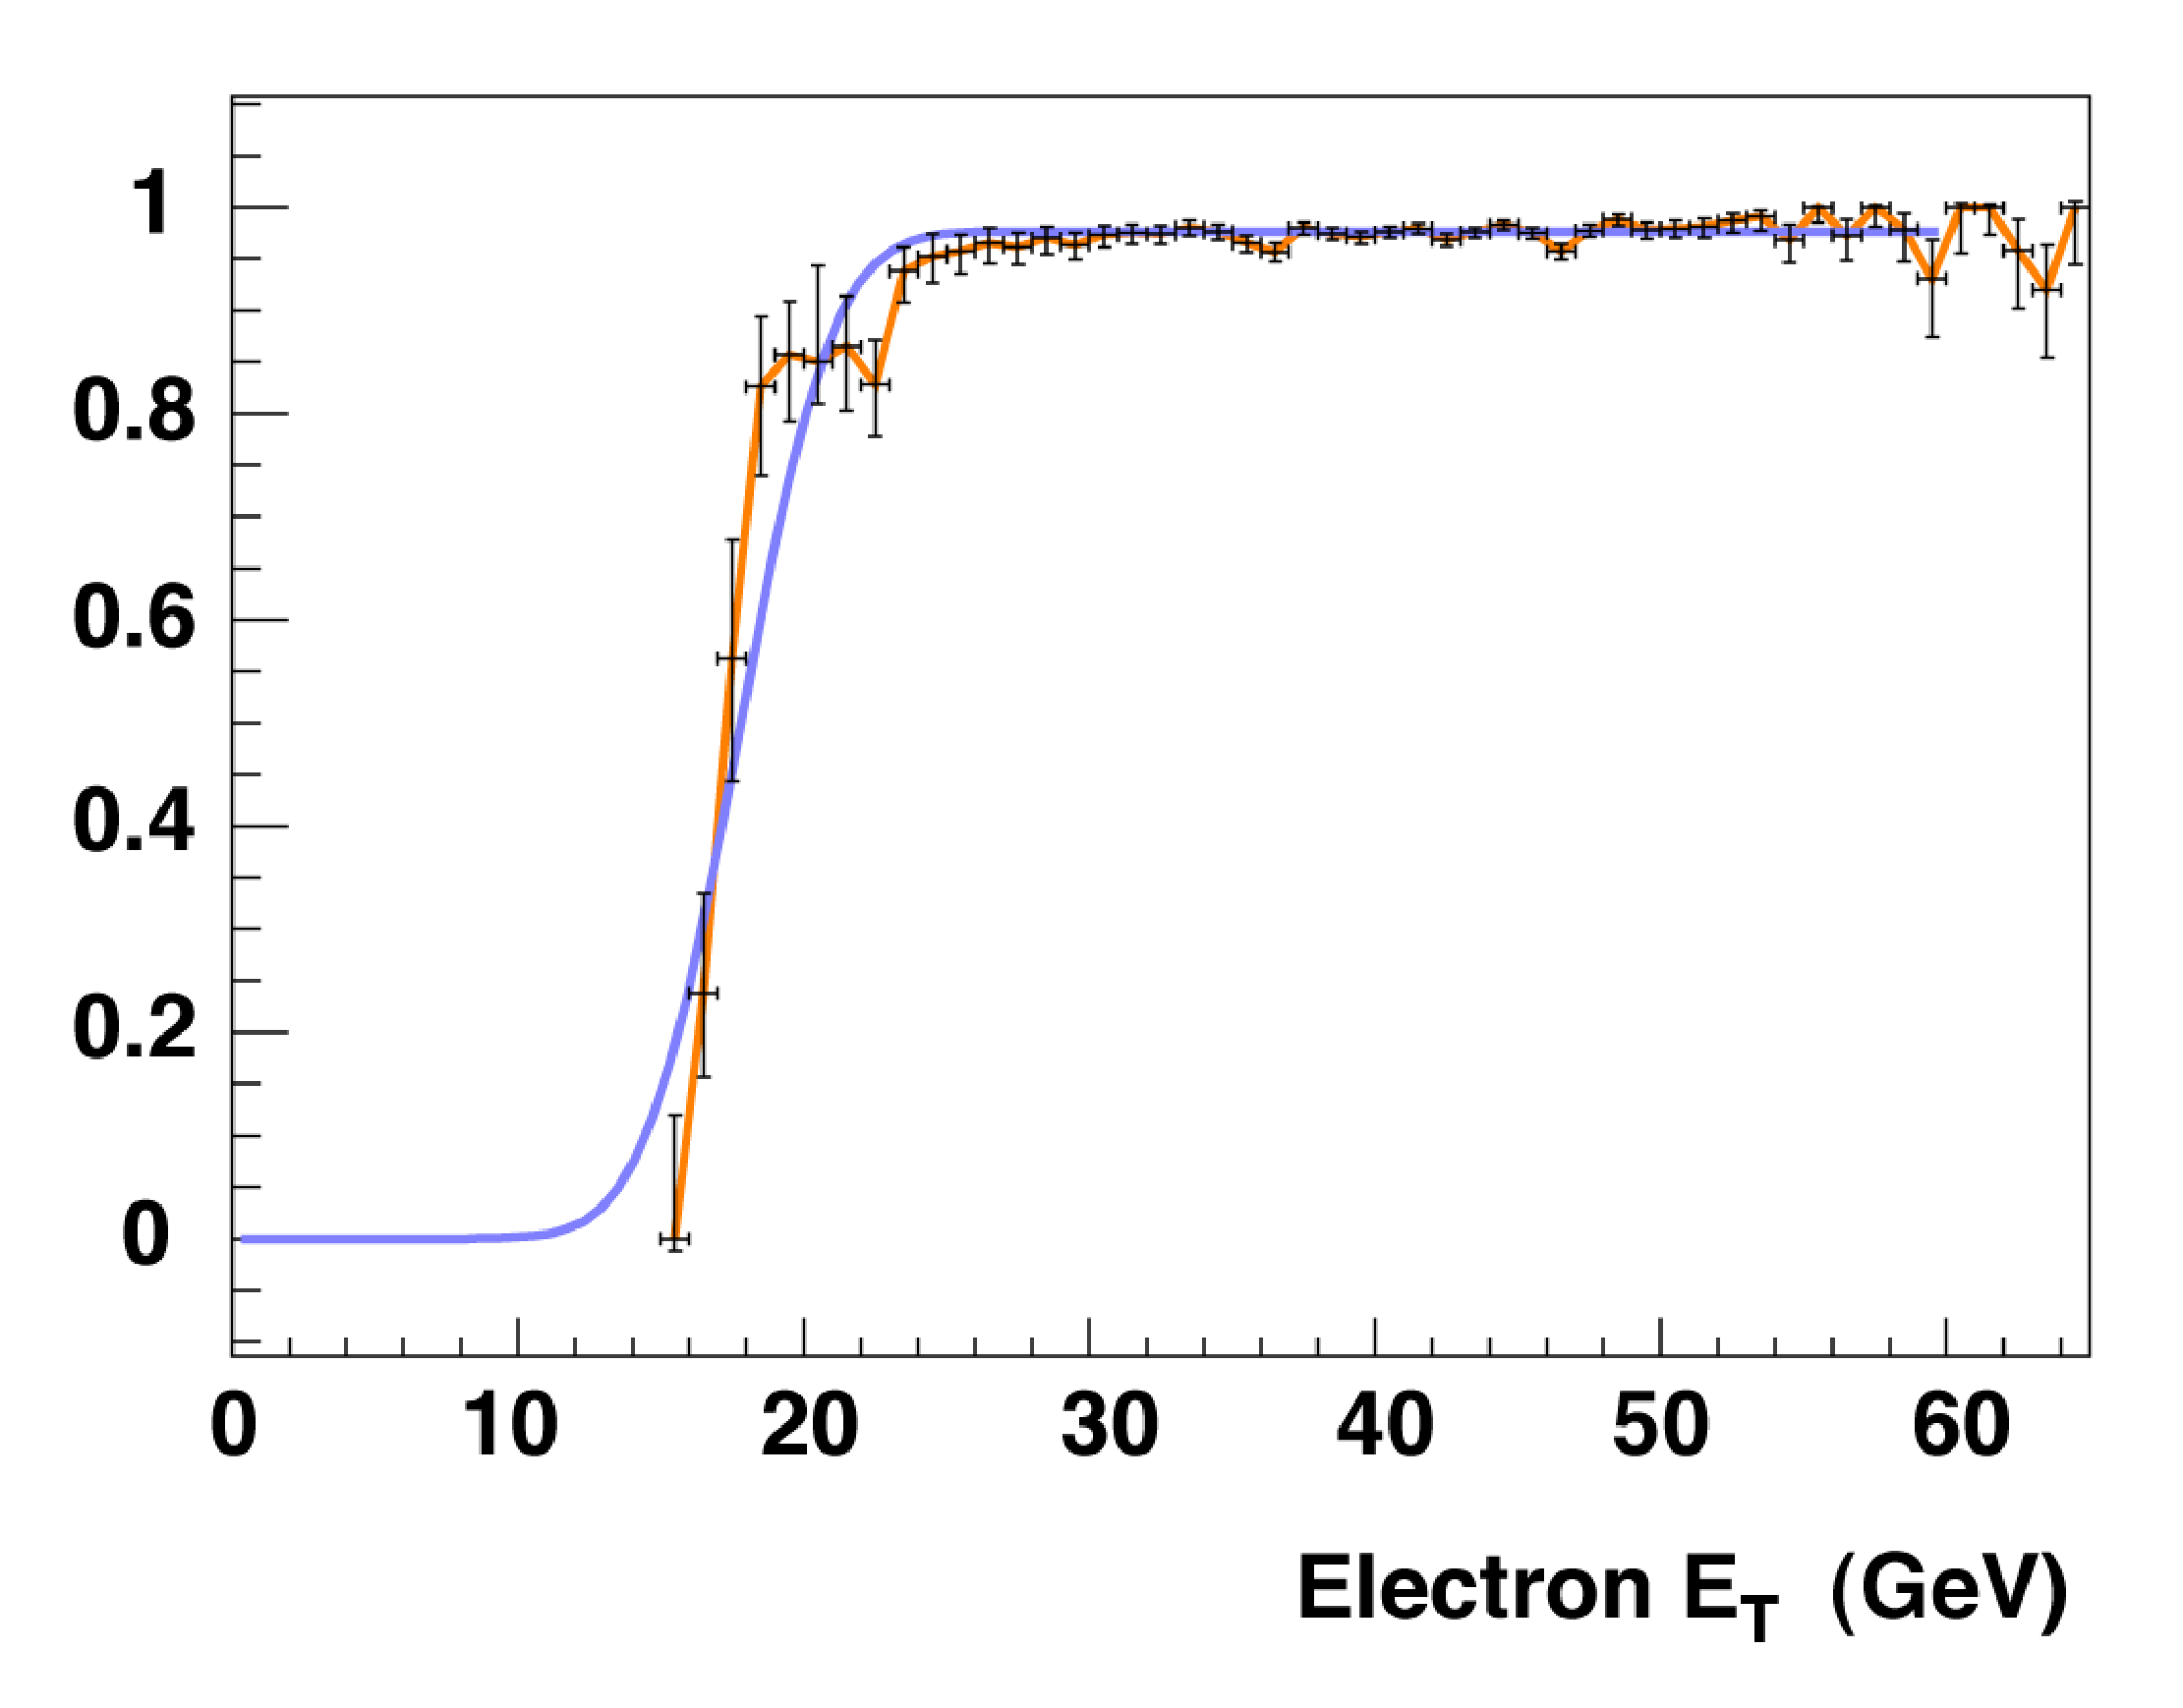
\includegraphics[width=0.49\textwidth]{eps/Reco/electron_turn-on_curve_pt.eps}
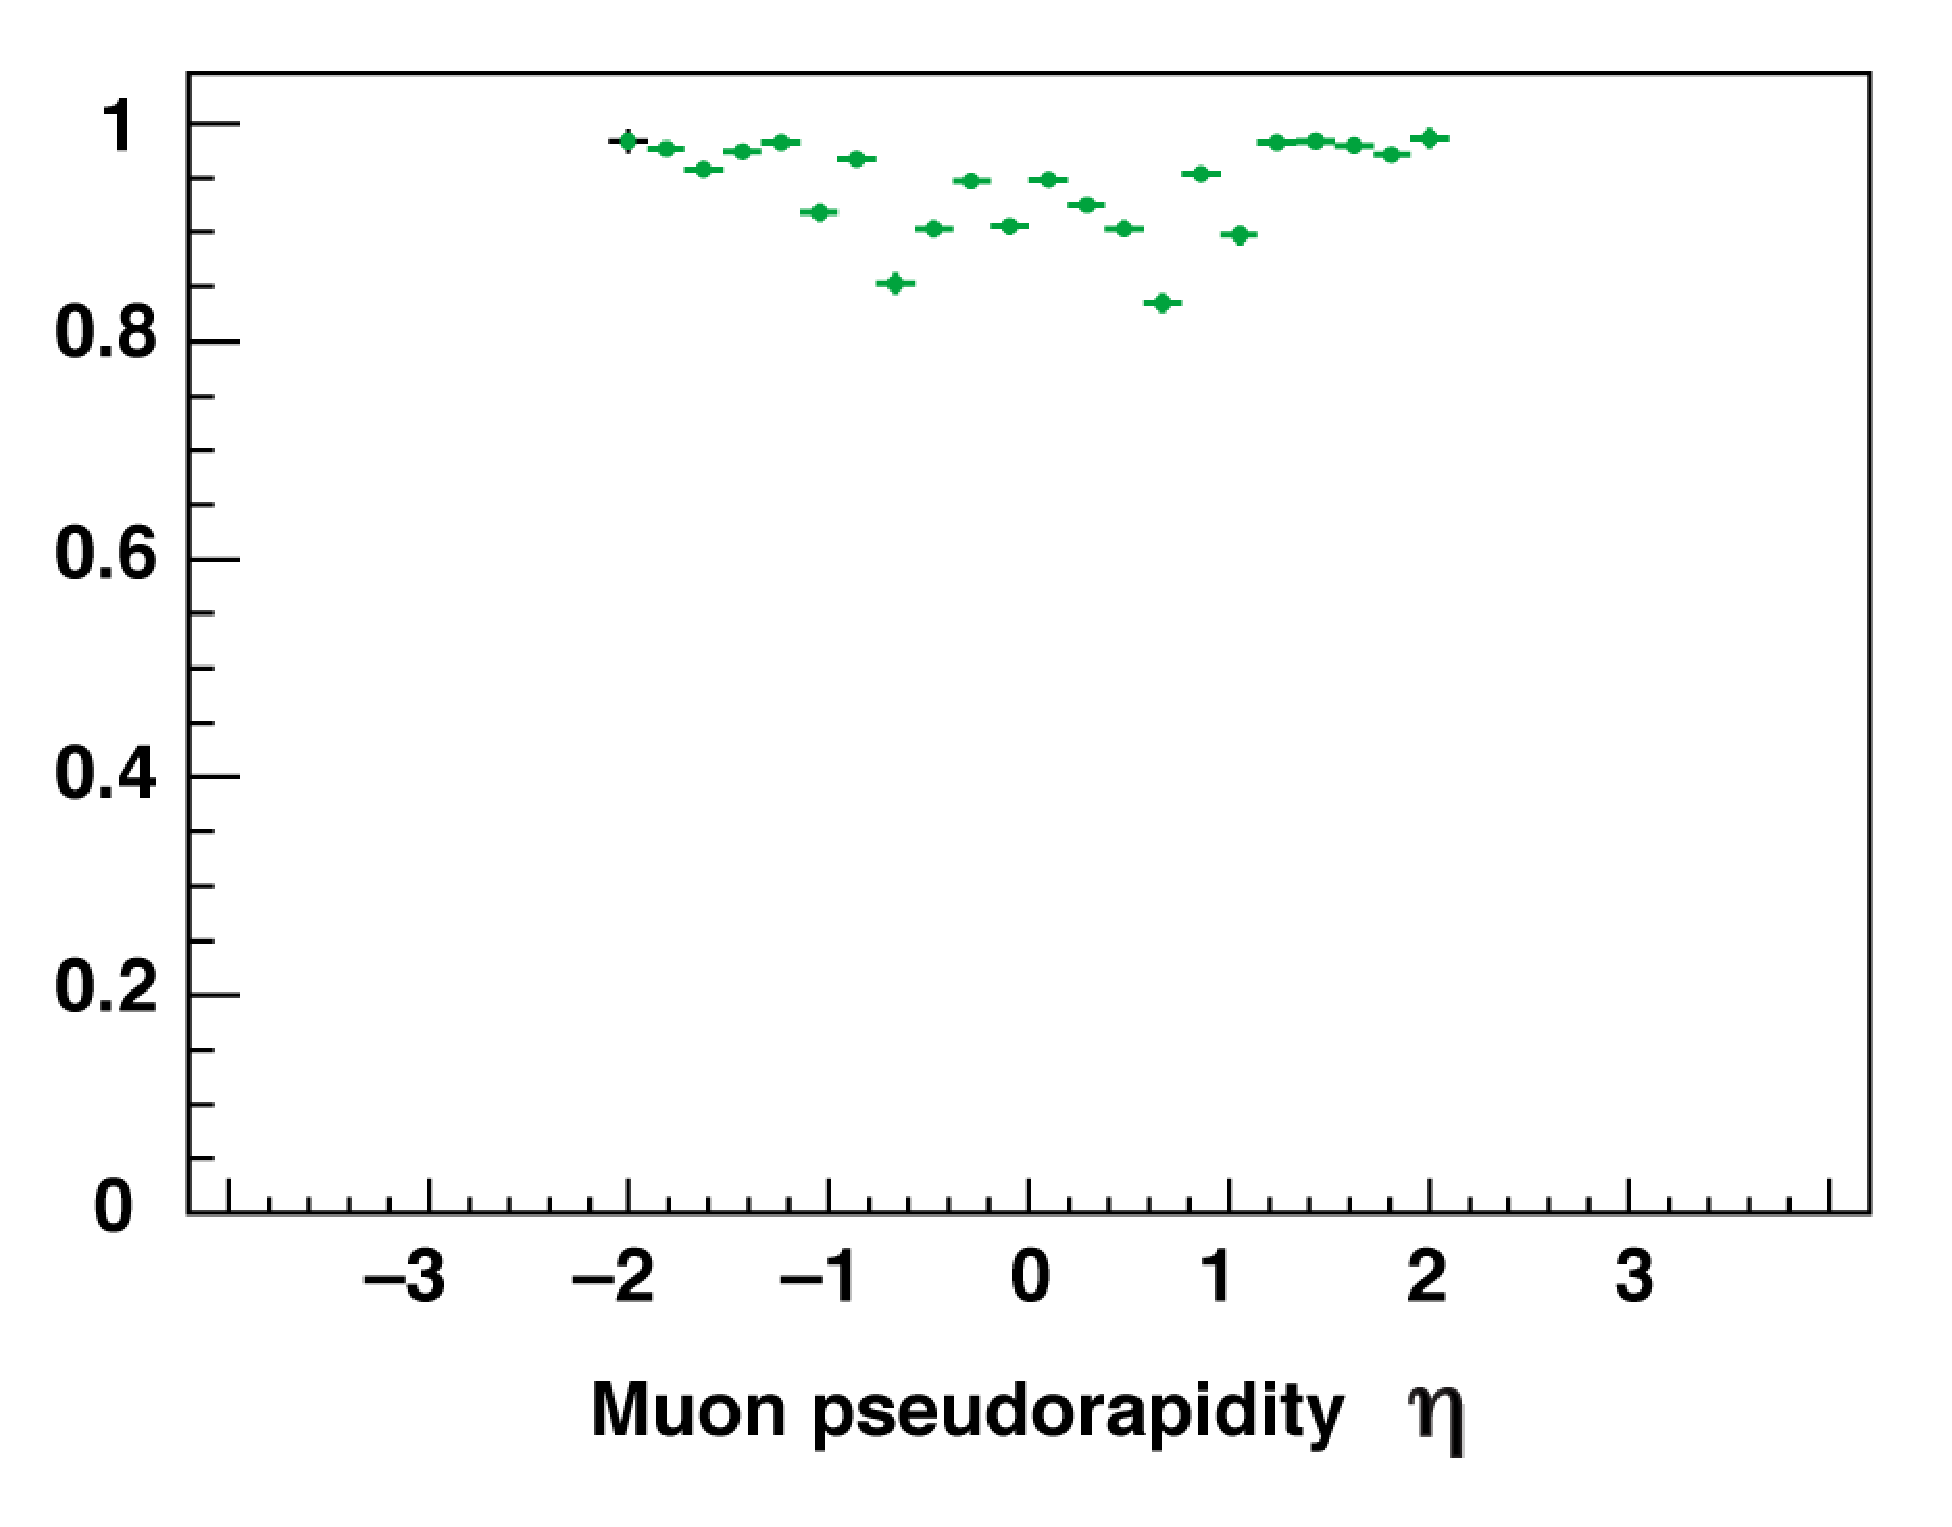
\includegraphics[width=0.49\textwidth]{eps/Reco/muon_turn-on_curve_eta.eps}
\end{center}
\vspace{-0.1in}
\caption{An example electron turn-on curve measured
as a function of the electron $p_{T}$ (left) and
an example muon turn-on curve measured as a function of $\eta$ (right). The points are trigger efficiencies derived from data
in that bin (with uncertainty bars)~\cite{singletopnote}.}
\label{triggereffexample}
\end{figure}


\section{Monte Carlo Corrections}
\label{corrections}

The result of the Monte Carlo generation with a full detector simulation are events that mimic real data events recorded by the $\dzero$~detector. Typically, however, the simulation is not complete for reasons such as missing material in the GEANT simulation or un-modeled aging effects of the detector. The result of not modeling these effects typically leads to an overestimation of detector resolution in the Monte Carlo. To account for this the reconstructed Monte Carlo objects are typically ``smeared" in one variable to ensure similar resolutions as is seen in data events. After the Monte Carlo events are smeared the relative difference between Monte Carlo and data events is measured and used to further correct the Monte Carlo. The following sections describe the smearing and correction factors for all reconstructed objects.


\subsection{Muons}

Muon smearing and correction factors are measured in $Z\rightarrow \mu\mu$ events because it provides a clean and unbiased sample of muons in both data and Monte Carlo. While the presence of a muon is confirmed by hits in the muon system the muon momentum vector is defined by the matched track. The muon track is defined by the charge and radius of curvature, which is proportional to $q/p_{T}$, thus the natural quantity to smear is $q/p_{T}$. The amount to which the muon track must be smeared is measured by observing the relative shift and width of the $Z$ boson resonance in data and Monte Carlo events. The functional form to which the muon track is smeared is shown in Eq.~\ref{muonsmear}.

\begin{equation}
\label{muonsmear}
\left( \frac{q}{p_{T}} \right)^{'} \rightarrow \frac{q}{p_{T}} + (A + \frac{B}{p_{T}})\times G
\end{equation}

\noindent The parameter $G$ is a random number generated from a Gaussian distribution centered at 0 and a width of 1. The parameters A and B are measured for muons with an SMT track hit in two regions ($\eta<1.6$ and $\eta>1.6$) and for muons without an SMT hit. Table~\ref{muonsmearparam} shows the smearing parameters for the three types of muons for two separate run periods.


\begin{table}[!h!tbp]
\begin{center}
\caption{Muon smearing parameters for the function $(A + \frac{B}{p_{T}})$ for two different run periods.}
\label{muonsmearparam}
\begin{tabular}{c|cc|cc|}
%\multicolumn{5}{c}
%{\underline{Muon Smearing Parameters}} \\
       & \multicolumn{2}{|c|}{$<$~Dec.~2004} & \multicolumn{2}{|c}{$>$~Dec.~2004} \\
Muon Type				&	A		&	B		&	A		&	B		\\
\hline
$>1$ SMT Hit ($\eta<1.6$)	&	0.00313	&	-0.0563	&	0.00308	&	-0.0370	\\
$>1$ SMT Hit ($\eta>1.6$)	&	0.00273	&	-0.0491	&	0.00458	&	-0.0550	\\
$=0$ SMT Hits				&	0.00509	&	-0.0916	&	0.00424	&	-0.0509	\\
\end{tabular}
\vspace{-0.1 in}
\end{center}
\end{table} 


After the smearing is applied the correction factor for muons is defined as the product of three independent factors, as shown in Eq.~\ref{muonscalefactor}, for reconstruction, track matching, and isolation.

\begin{equation}
\label{muonscalefactor}
f_{\rm{Data/MC}}(\mu) = \frac{\varepsilon^{\rm{Data}}_{\rm{Reco}}(\mu)}{\varepsilon^{\rm{MC}}_{\rm{Reco}}(\mu)} \times 
\frac{\varepsilon^{\rm{Data}}_{\rm{Track|Reco}}(\mu)}{\varepsilon^{\rm{MC}}_{\rm{Track|Reco}}(\mu)} \times \frac{\varepsilon^{\rm{Data}}_{\rm{Isolation|Track}}(\mu)}{\varepsilon^{\rm{MC}}_{\rm{Isolation|Track}}(\mu)}
\end{equation}

The muon reconstruction efficiency for data and the Monte Carlo correction factor are shown in Fig.~\ref{muonrecoeffscale}. The empty region in the center of the $\eta$-$\phi$ efficiency histogram corresponds to the hole in the bottom of the muon detector. The correction factor is only considered to be a function of $\eta$ since the reconstruction efficiencies for data and Monte Carlo show the same $\phi$ dependence. The average reconstruction efficiency in data is 80.2$\%$ and the average Monte Carlo correction factor is $0.97$.

\begin{figure}[!h!tbp]
\begin{center}
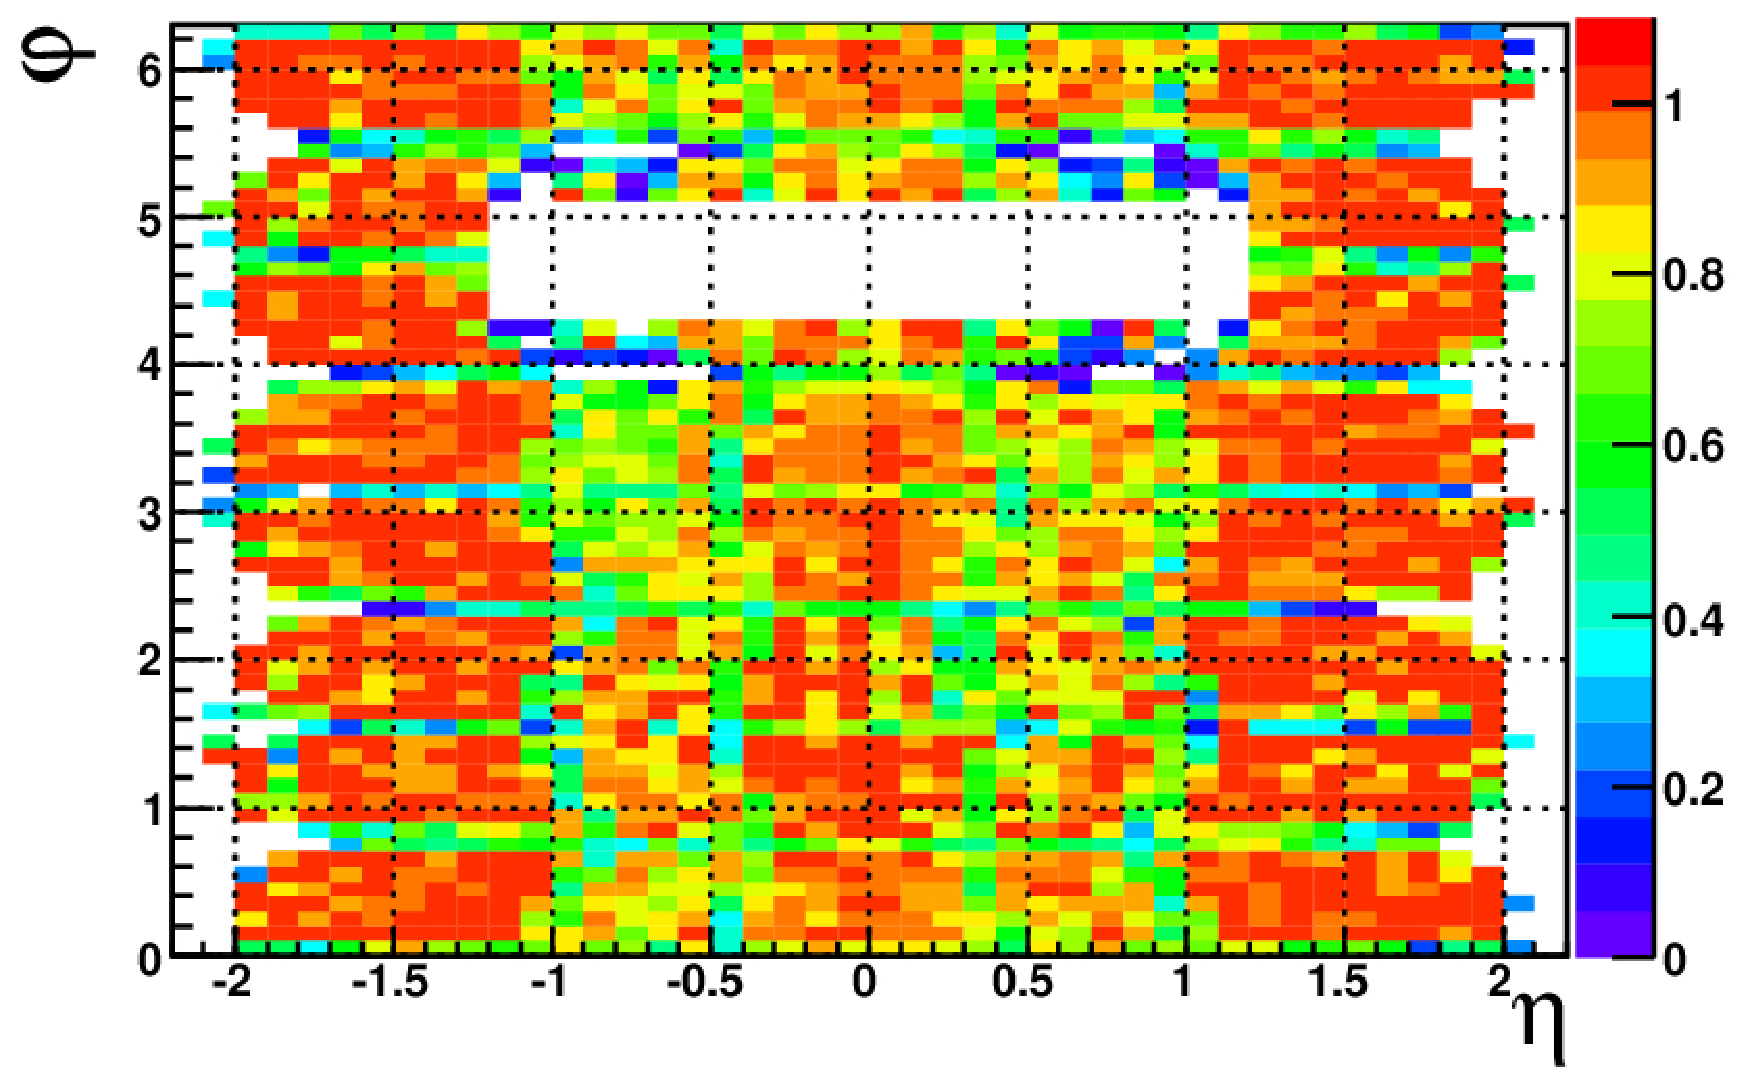
\includegraphics[width=0.49\textwidth]{eps/Reco/muonreco.eps}
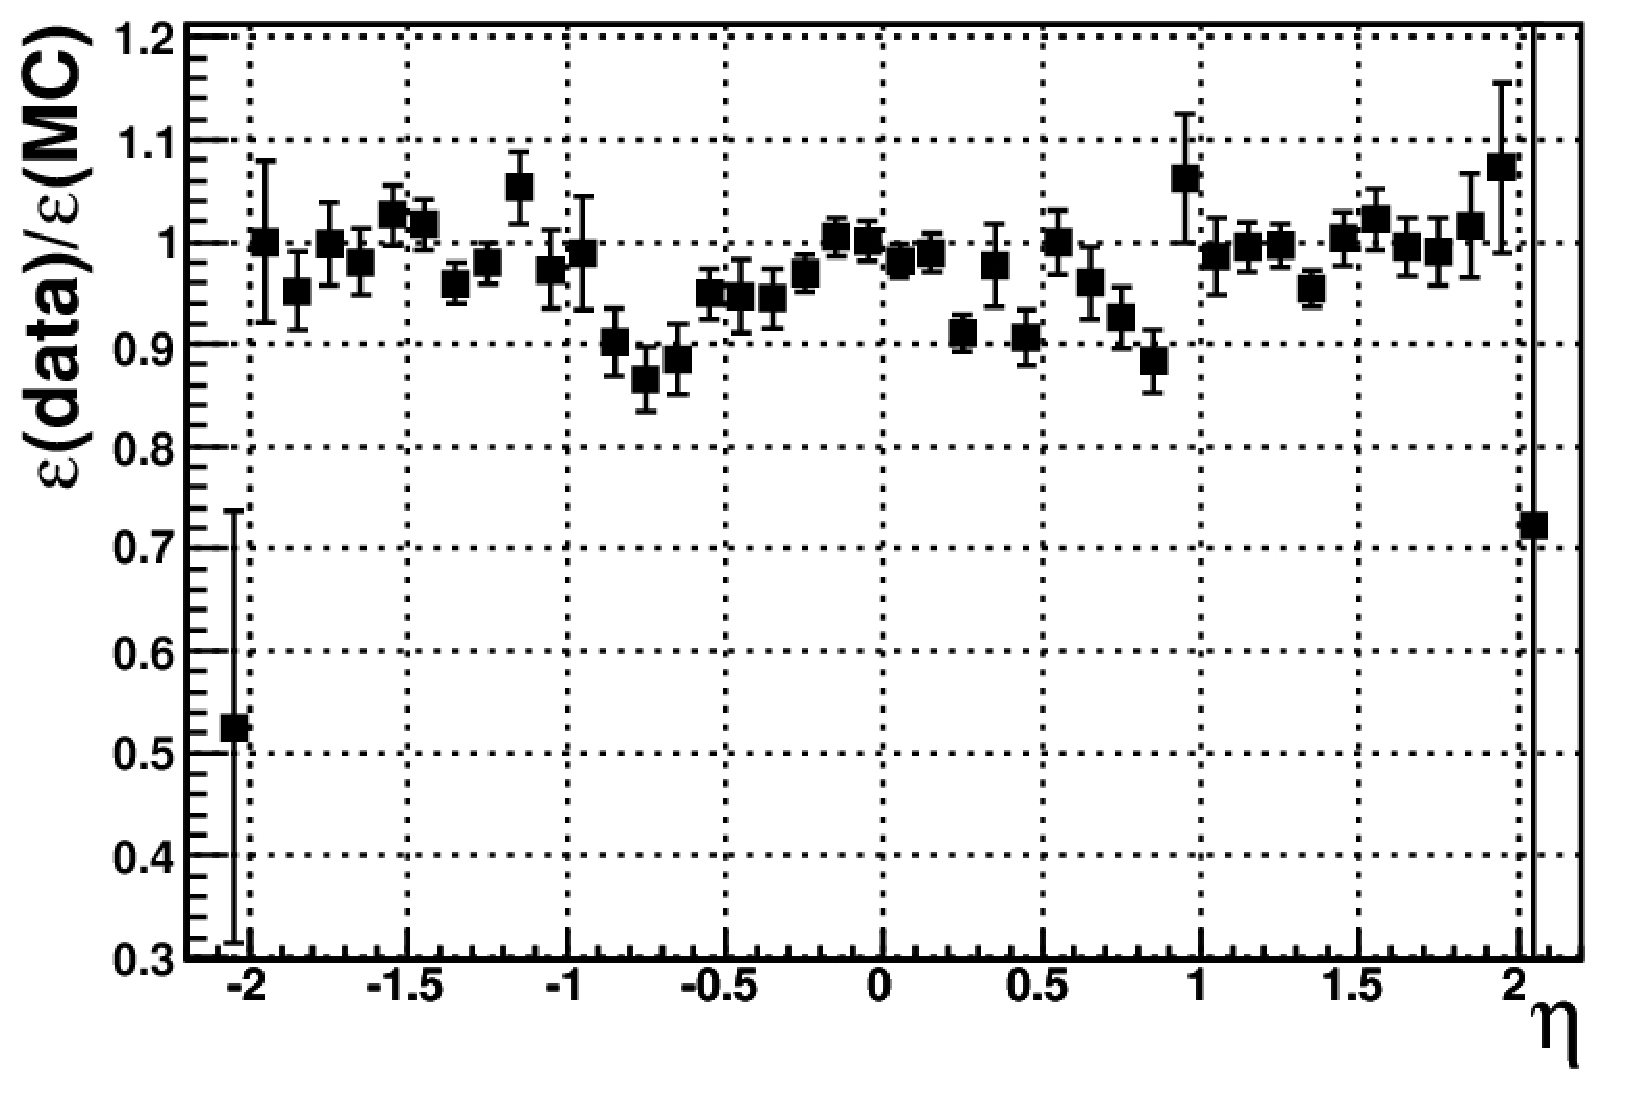
\includegraphics[width=0.49\textwidth]{eps/Reco/muonrecoscale.eps}
\end{center}
\vspace{-0.1in}
\caption{Muon reconstruction efficiency as measured in $Z\rightarrow \mu\mu$ data events (left) and the Monte Carlo correction factor as a function of muon $\eta$ (right)~\cite{muon}.}
\label{muonrecoeffscale}
\end{figure}

The muon track match efficiency is measured with respect to reconstructed muons. The efficiency is found to depend on two tracking related quantities, the track $\eta$ and the longitudinal primary interaction vertex position. The efficiency in data and correction factor are shown in Fig.~\ref{muontrackeffscale}. The average track match efficiency in data is 91.0$\%$ and the average Monte Carlo correction factor is $0.93$.

\begin{figure}[!h!tbp]
\begin{center}
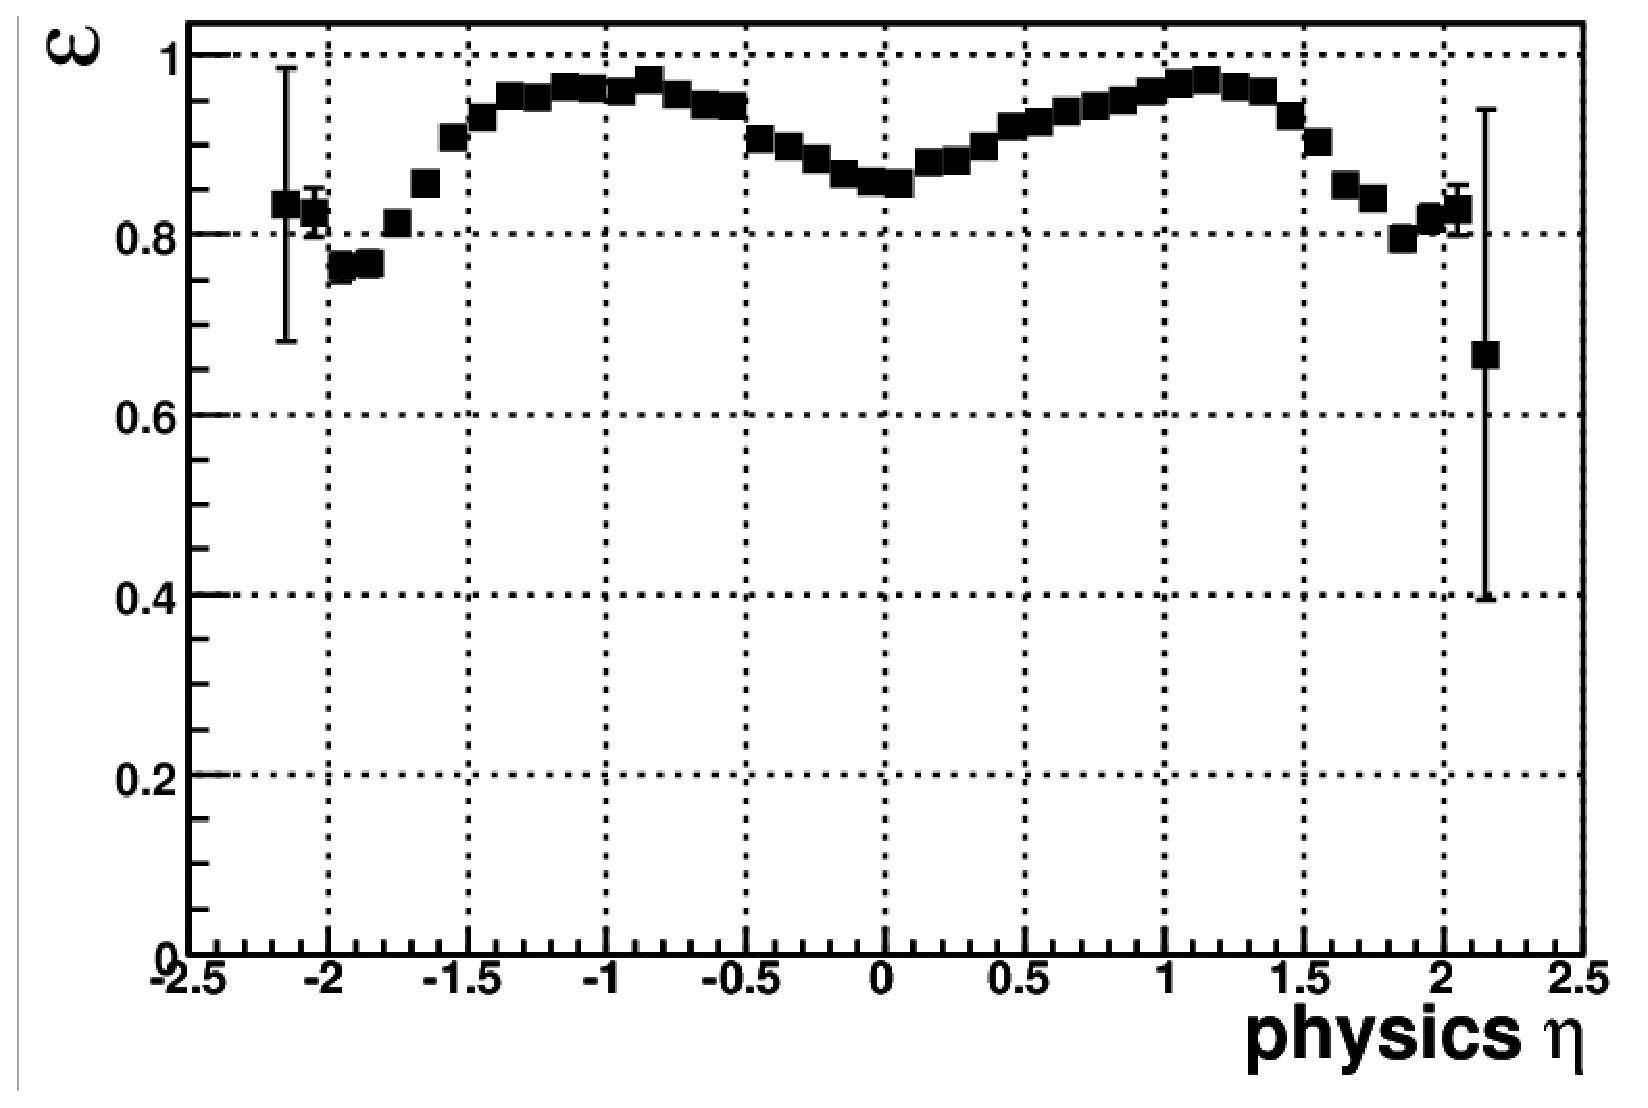
\includegraphics[width=0.49\textwidth]{eps/Reco/muontrack.eps}
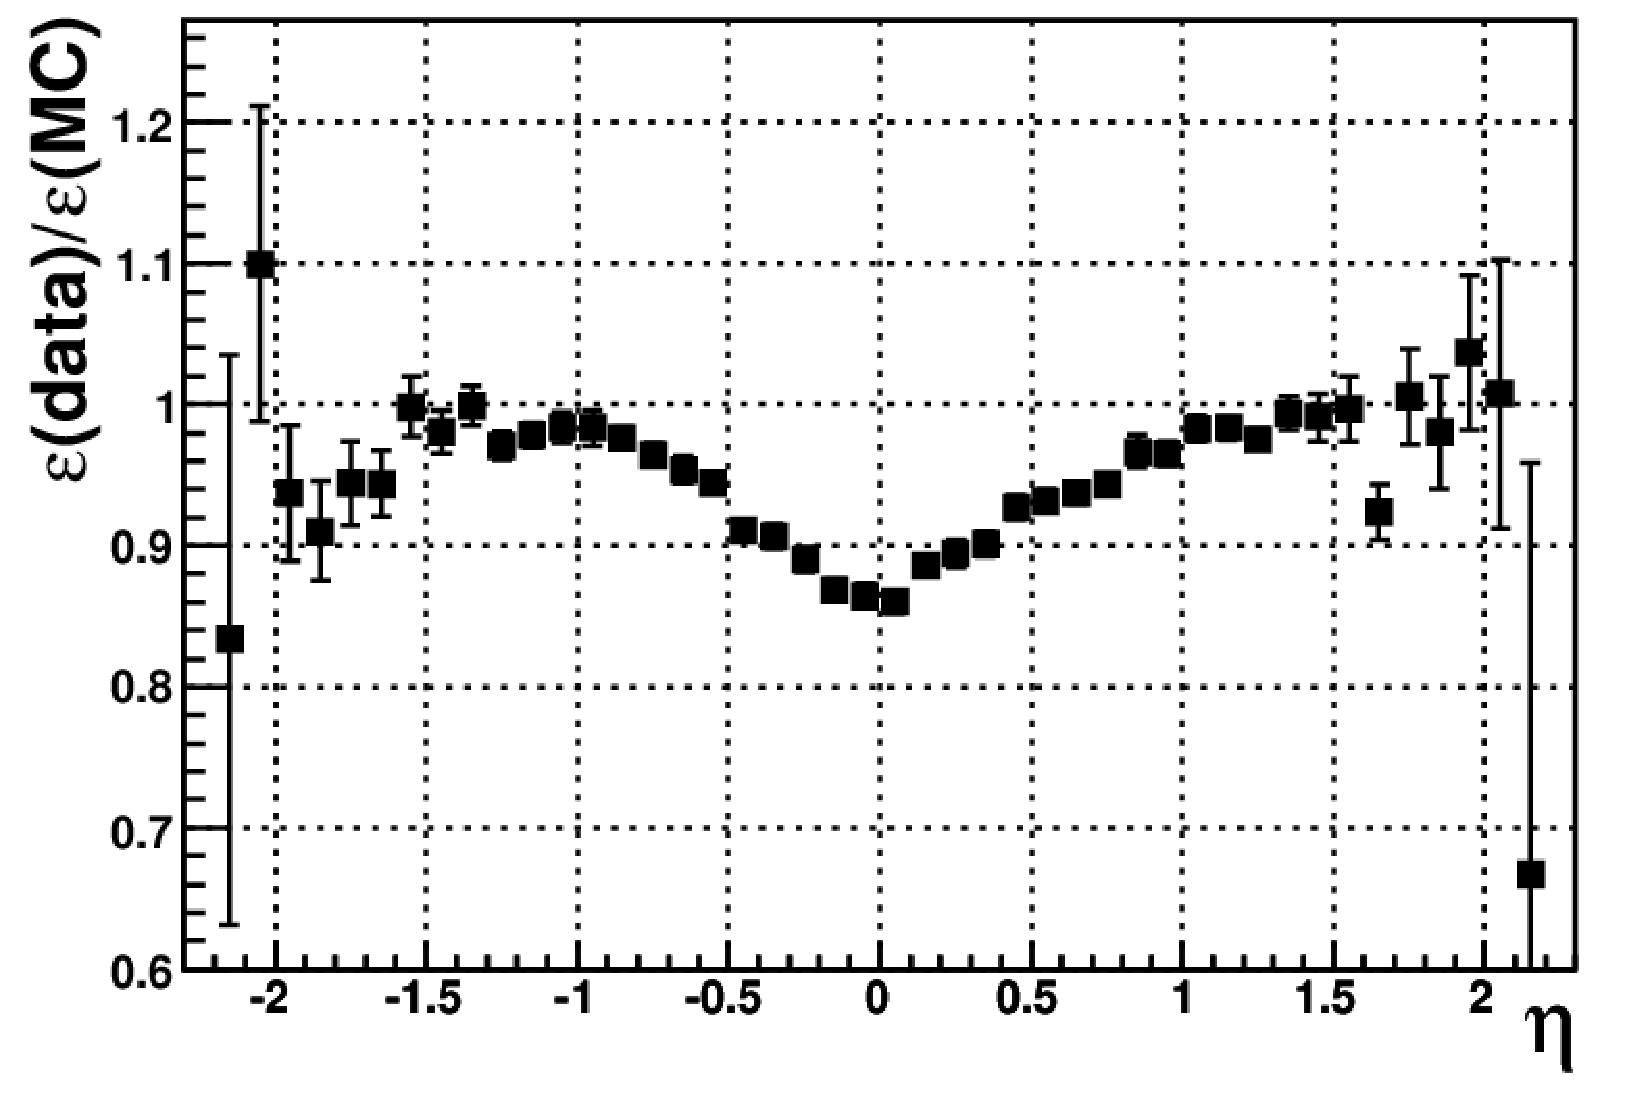
\includegraphics[width=0.49\textwidth]{eps/Reco/muontrackscale.eps}
\end{center}
\vspace{-0.1in}
\caption{Muon track match efficiency as measured in $Z\rightarrow \mu\mu$ data events (left) and the Monte Carlo correction factor as a function of track $\eta$ (right)~\cite{muon}.}
\label{muontrackeffscale}
\end{figure}

The muon isolation efficiency is measured in $Z\rightarrow\mu\mu$ events for reconstructed muon with a confirmed track match. The isolation efficiency depends most strongly on the number of reconstructed jets in the event since it is more difficult for a muon to be isolated if the jets occupy more space in the detector. Fig.~\ref{muonisoeffscale} shows the isolation efficiency and Monte Carlo correction factor as a function of the jet multiplicity. The Monte Carlo correction factor for events with two or three jets, such as single top quark events, is $0.98$, with an average efficiency of $0.94\%$.

\begin{figure}[!h!tbp]
\begin{center}
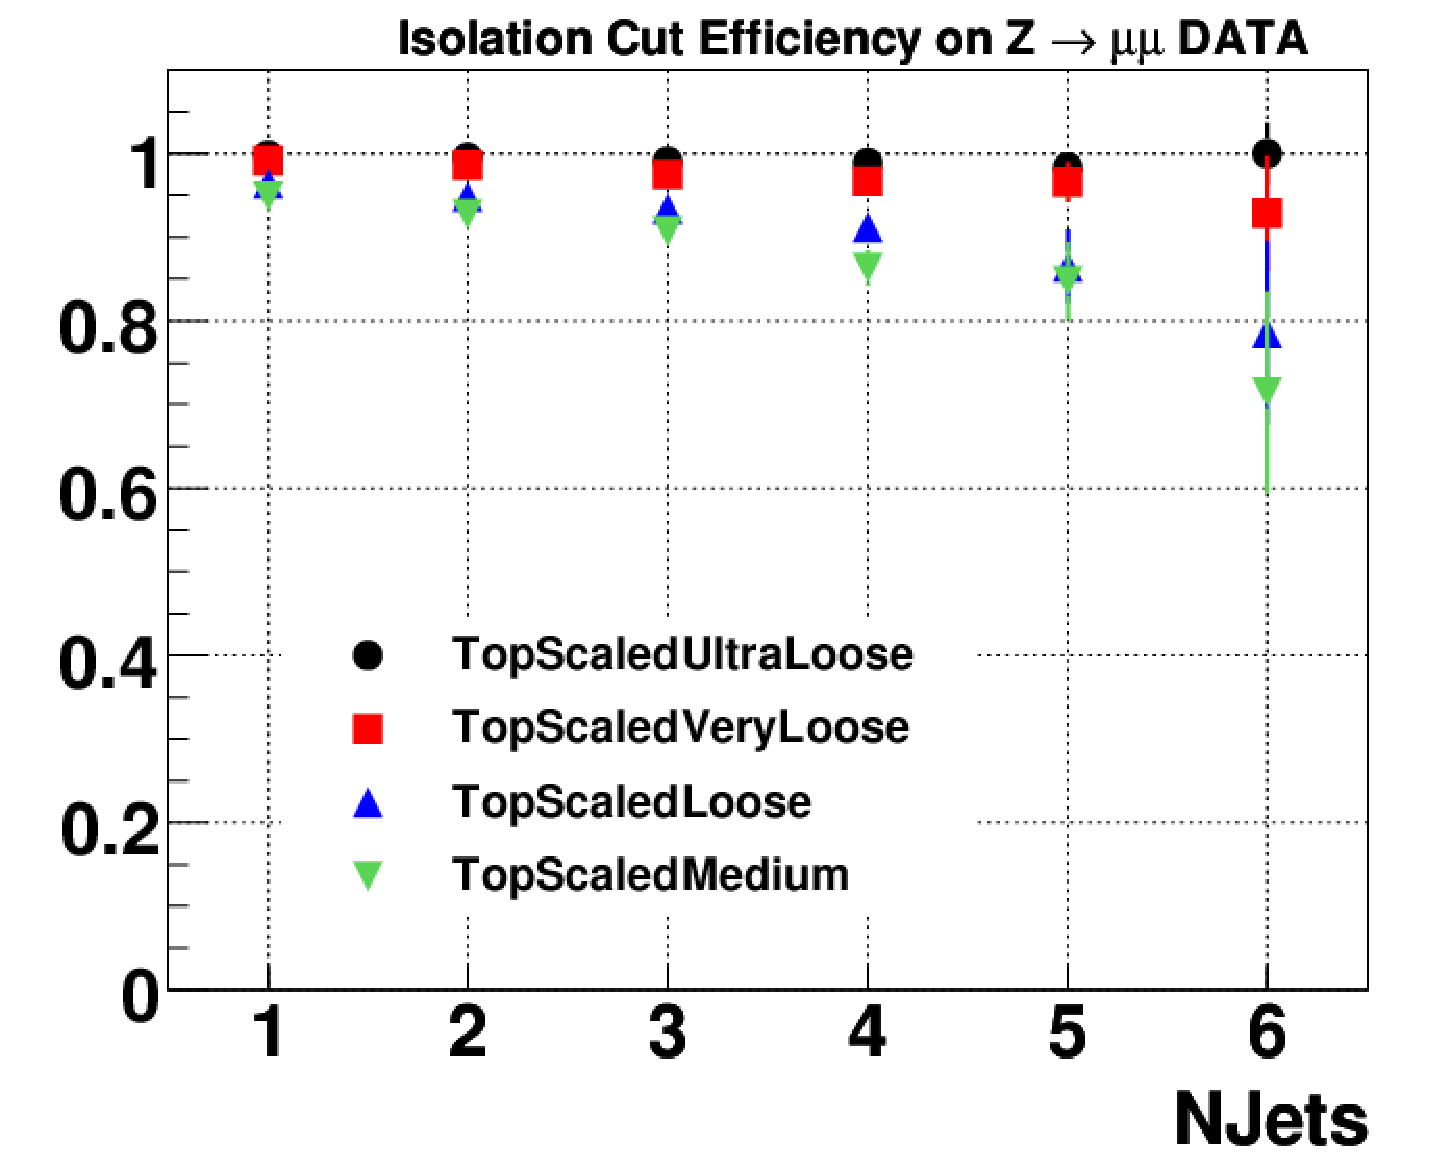
\includegraphics[width=0.49\textwidth]{eps/Reco/muoniso.eps}
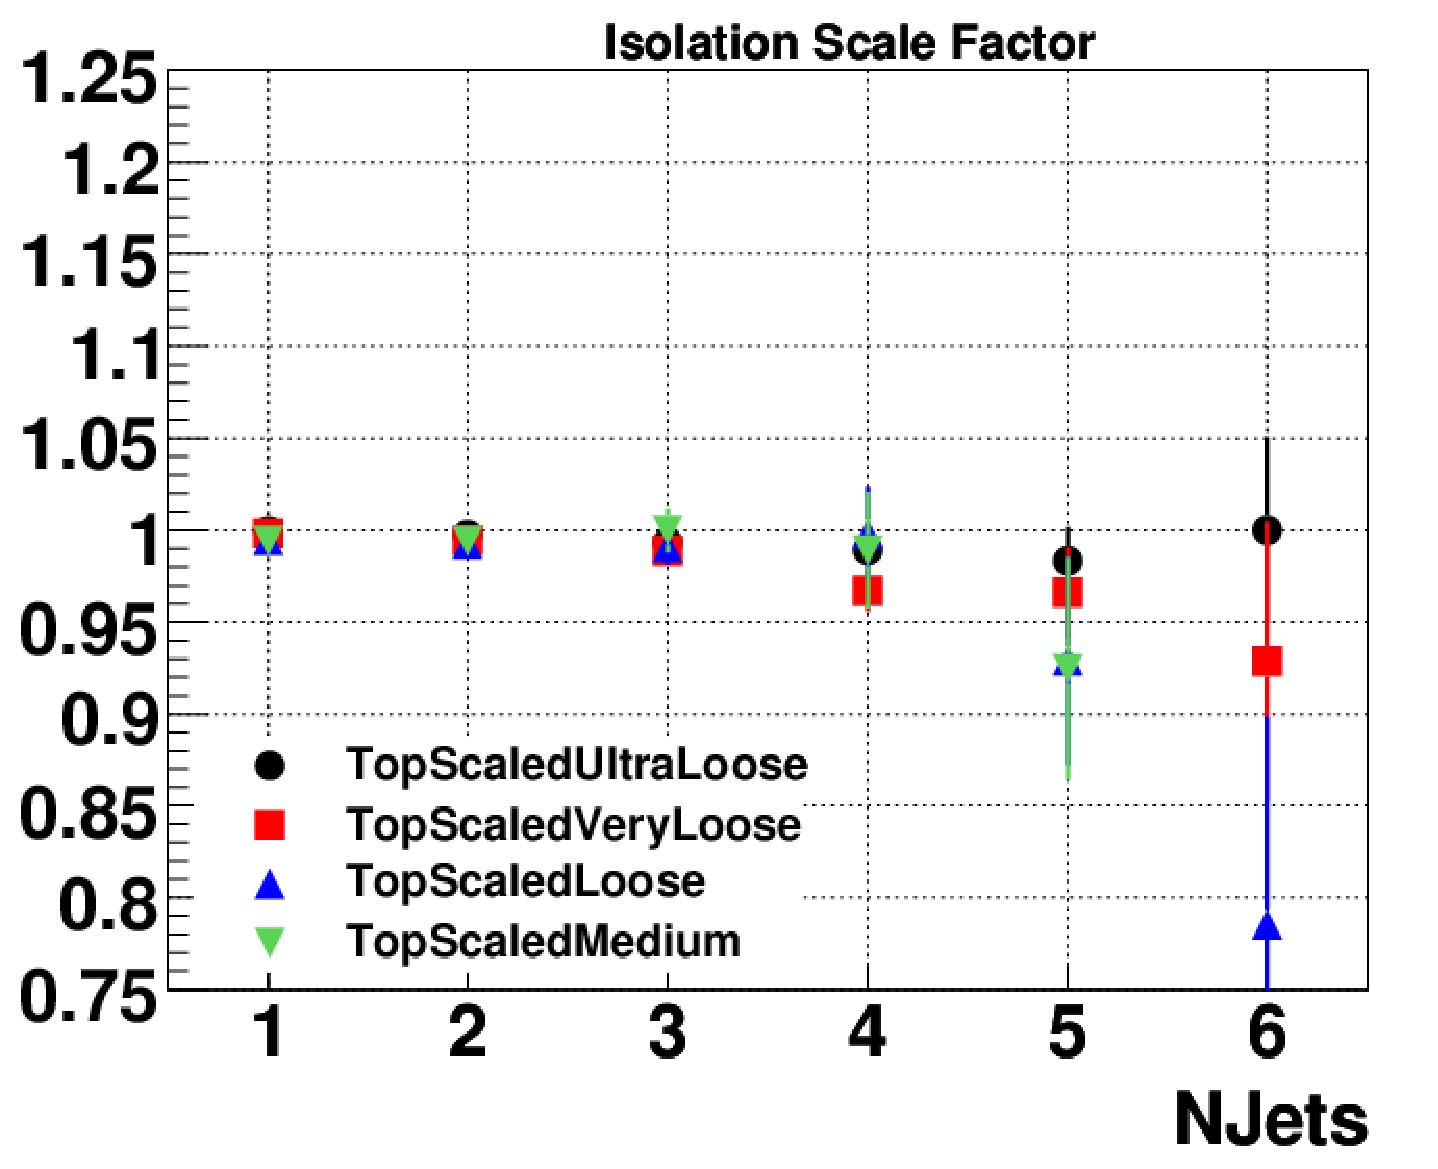
\includegraphics[width=0.49\textwidth]{eps/Reco/muonisoscale.eps}
\end{center}
\vspace{-0.1in}
\caption{Muon isolation efficiency as measured in $Z\rightarrow \mu\mu$ data events for various regions of primary vertex $z$ position (left) and Monte Carlo correction factor as a function of the number of reconstructed jets. The isolation used in the single top quark analysis is labeled TopScaledLoose and corresponds to the blue triangle curve~\cite{muon}.}
\label{muonisoeffscale}
\end{figure}


\subsection{Electrons}

There is no smearing applied to Monte Carlo electrons since the resolution is well-modeled in the Monte Carlo. Electron correction factors are measured in $Z\rightarrow ee$ data and Monte Carlo events. The correction factor for electrons is considered a product of two independent factors: reconstruction and track match plus likelihood cuts, as shown in Eq.~\ref{electronscalefactor}.

\begin{equation}
\label{electronscalefactor}
f_{\rm{Data/MC}}(e) = \frac{\varepsilon^{\rm{Data}}_{\rm{Reco}}(e)}{\varepsilon^{\rm{MC}}_{\rm{Reco}}(e)} \times 
\frac{\varepsilon^{\rm{Data}}_{\rm{TrackMatchLikelihood|Reco}}(e)}{\varepsilon^{\rm{MC}}_{\rm{TrachMatchLikelihood|Reco}}(e)}
\end{equation}

Electron reconstruction efficiencies as measured in $Z\rightarrow ee$ data and Monte Carlo events and the Monte Carlo correction factor show a slight $p_{T}$ dependence as seen in Fig.~\ref{electronrecoeffscale}.

\begin{figure}[!h!tbp]
\begin{center}
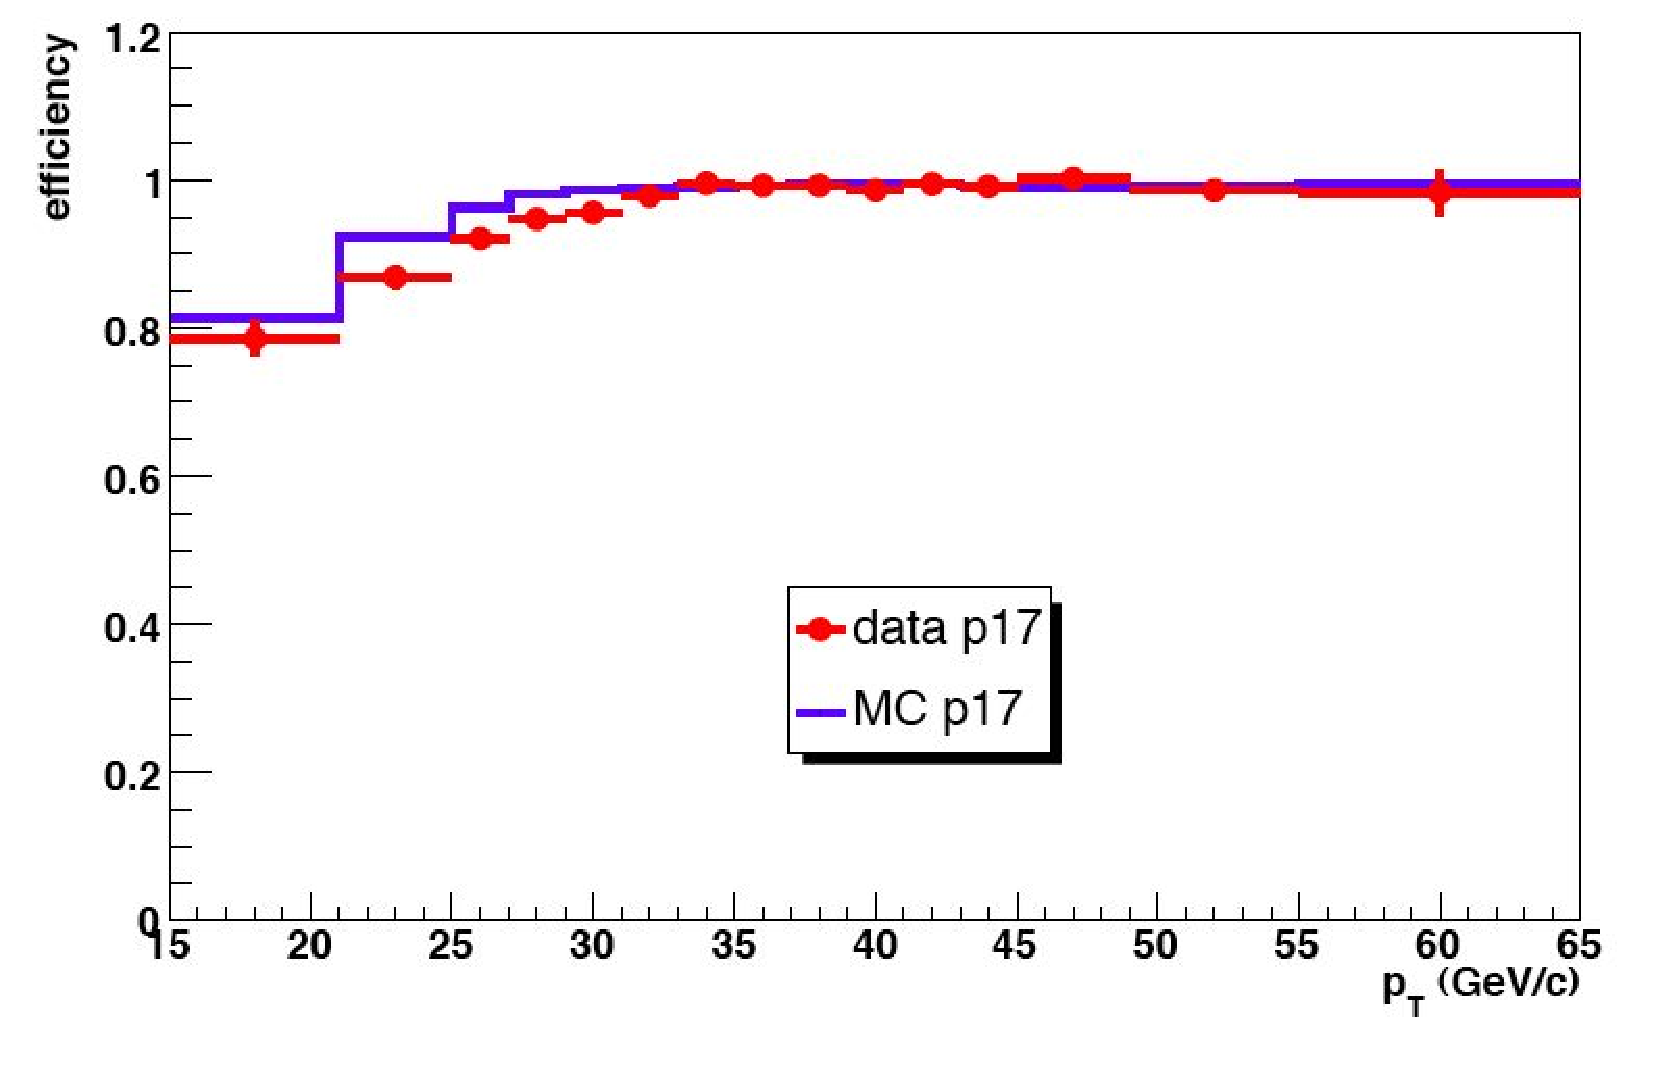
\includegraphics[width=0.49\textwidth]{eps/Reco/Electron_Reco_eff.eps}
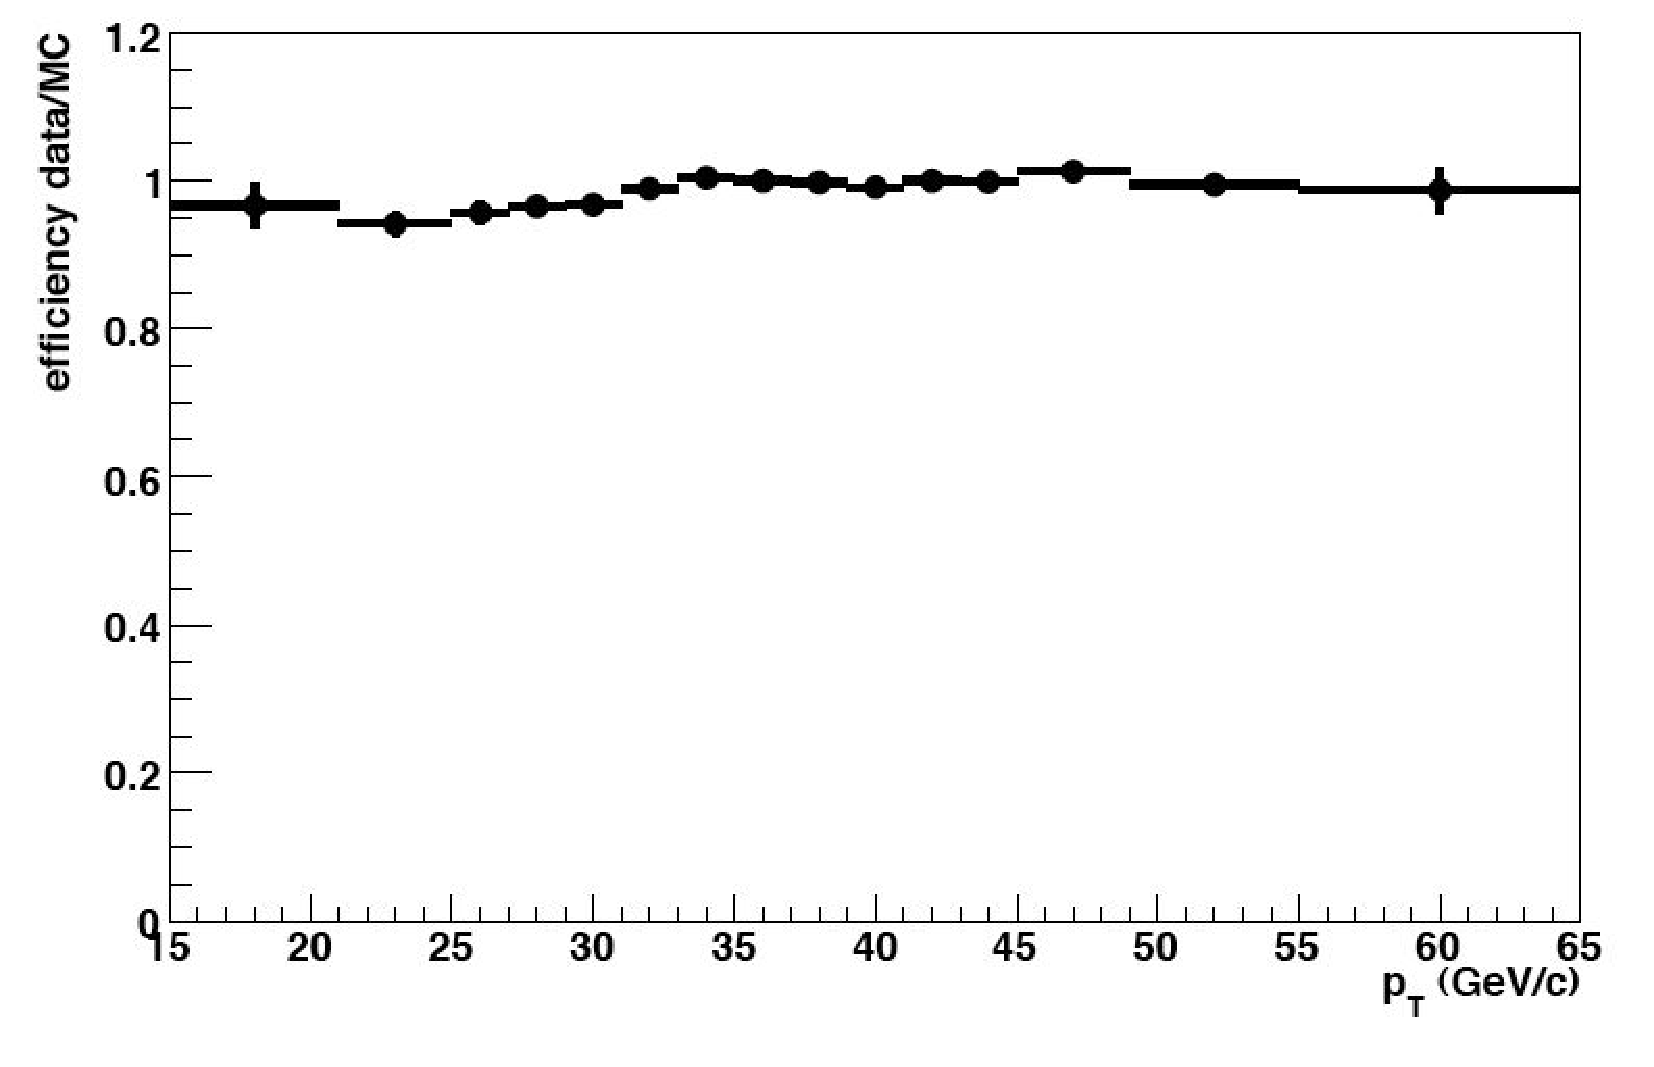
\includegraphics[width=0.49\textwidth]{eps/Reco/Electron_Reco_scale.eps}
\end{center}
\vspace{-0.1in}
\caption{Electron reconstruction efficiency as measured in $Z\rightarrow ee$ data (red) and Monte Carlo (blue) events (left) and Monte Carlo correction factor as a function of electron $p_{T}$ (right)~\cite{electron}.}
\label{electronrecoeffscale}
\end{figure}

Electron likelihood and track match efficiencies are measured in $Z\rightarrow ee$ data and Monte Carlo events with respect to reconstructed electrons. The efficiency in data and the Monte Carlo correction factor are shown in Fig.~\ref{electronlikelihoodeffscale}. The single top quark analysis only use electrons out to 1.1 in $\eta^{det}$.

\begin{figure}[!h!tbp]
\begin{center}
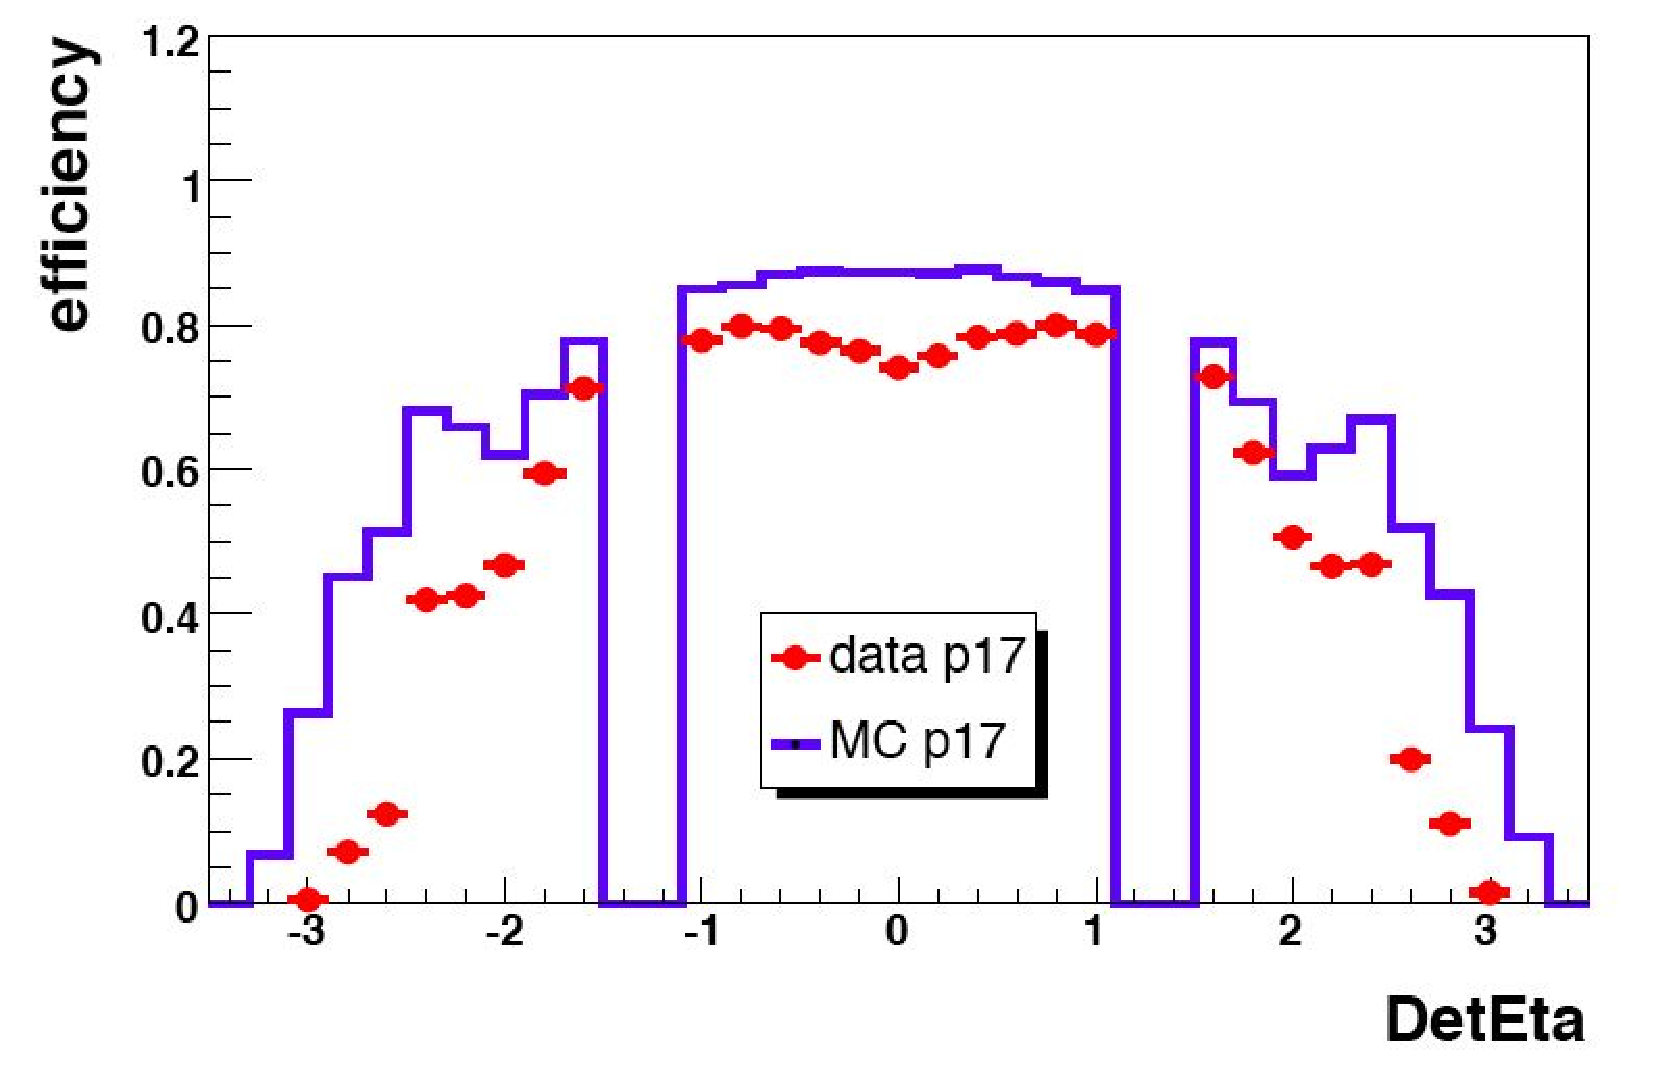
\includegraphics[width=0.49\textwidth]{eps/Reco/Electron_Likelihood_eff.eps}
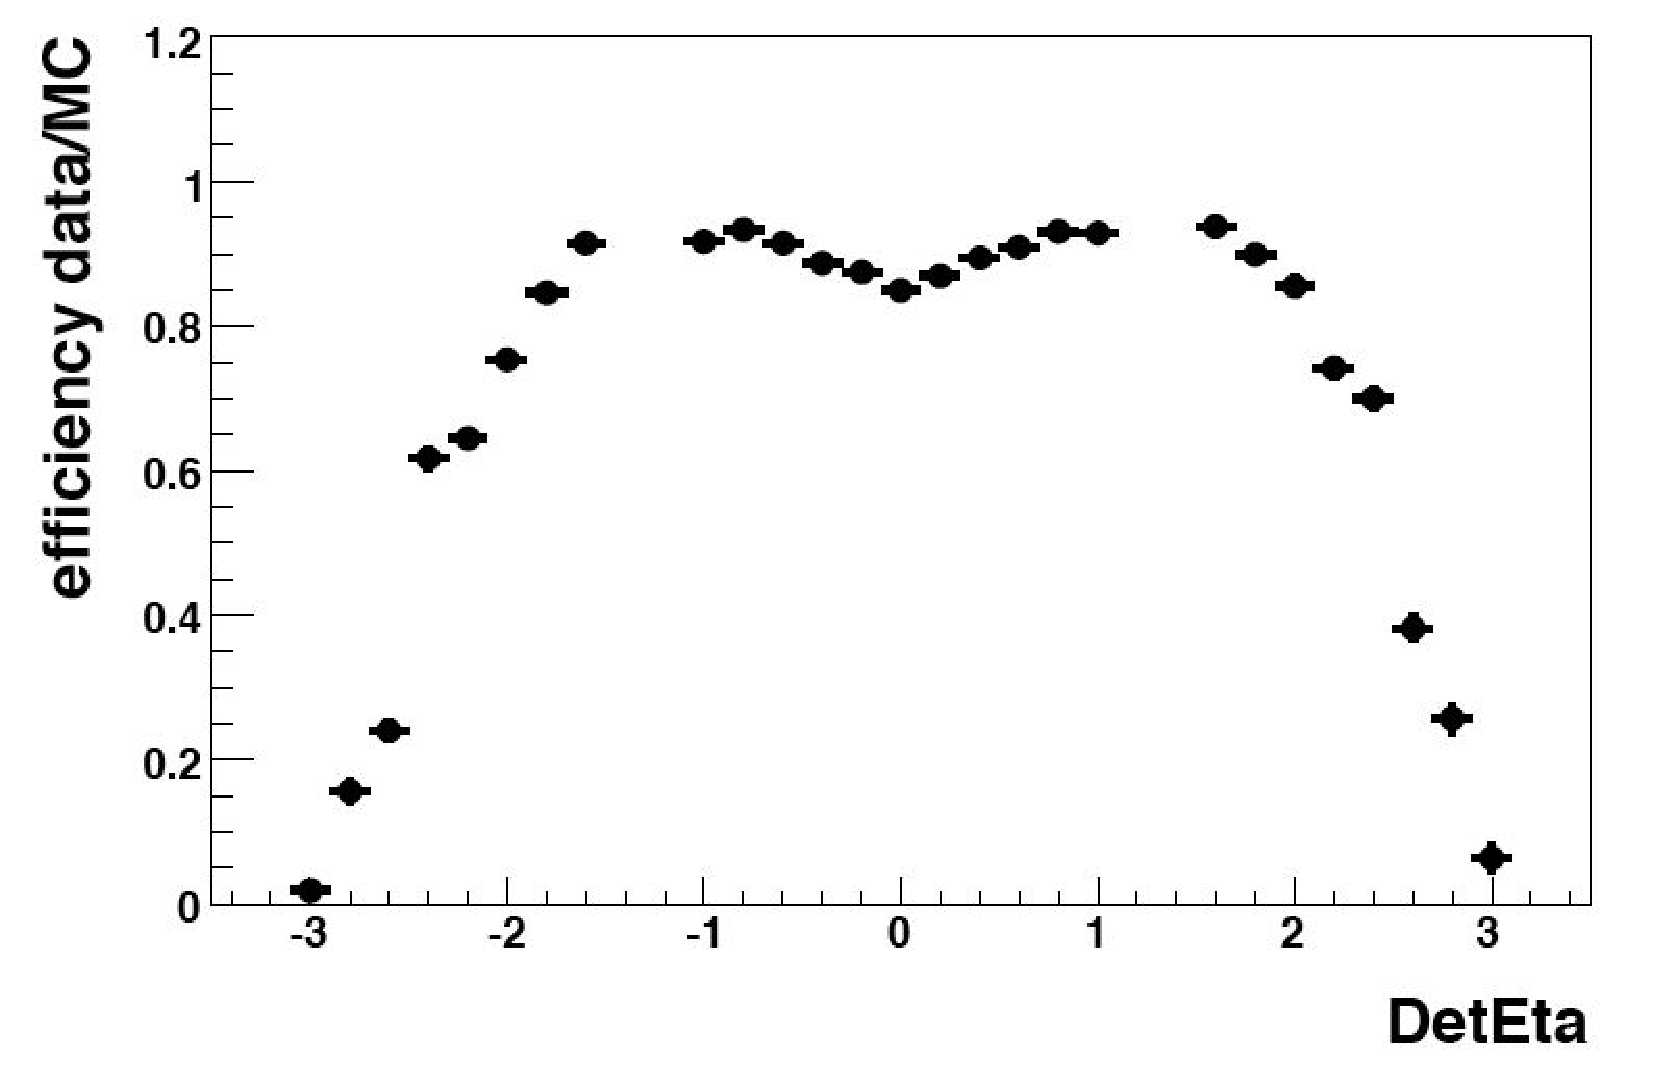
\includegraphics[width=0.49\textwidth]{eps/Reco/Electron_Likelihood_scale.eps}
\end{center}
\vspace{-0.1in}
\caption{Electron reconstruction efficiency as measured in $Z\rightarrow ee$ data (red) and Monte Carlo (blue) events (left) and Monte Carlo correction factor as a function of electron $p_{T}$ (right)~\cite{electron}.}
\label{electronlikelihoodeffscale}
\end{figure}

\subsection{Primary Interaction Vertex}

The primary interaction vertex efficiency is measured using $Z\rightarrow \mu\mu$ data and Monte Carlo events and the correction factor is defined as the ratio of the two efficiencies. The primary vertex reconstruction efficiency in data is shown in Fig.~\ref{pveff}. No correction to the Monte Carlo primary vertices is applied.

\begin{figure}[!h!tbp]
\begin{center}
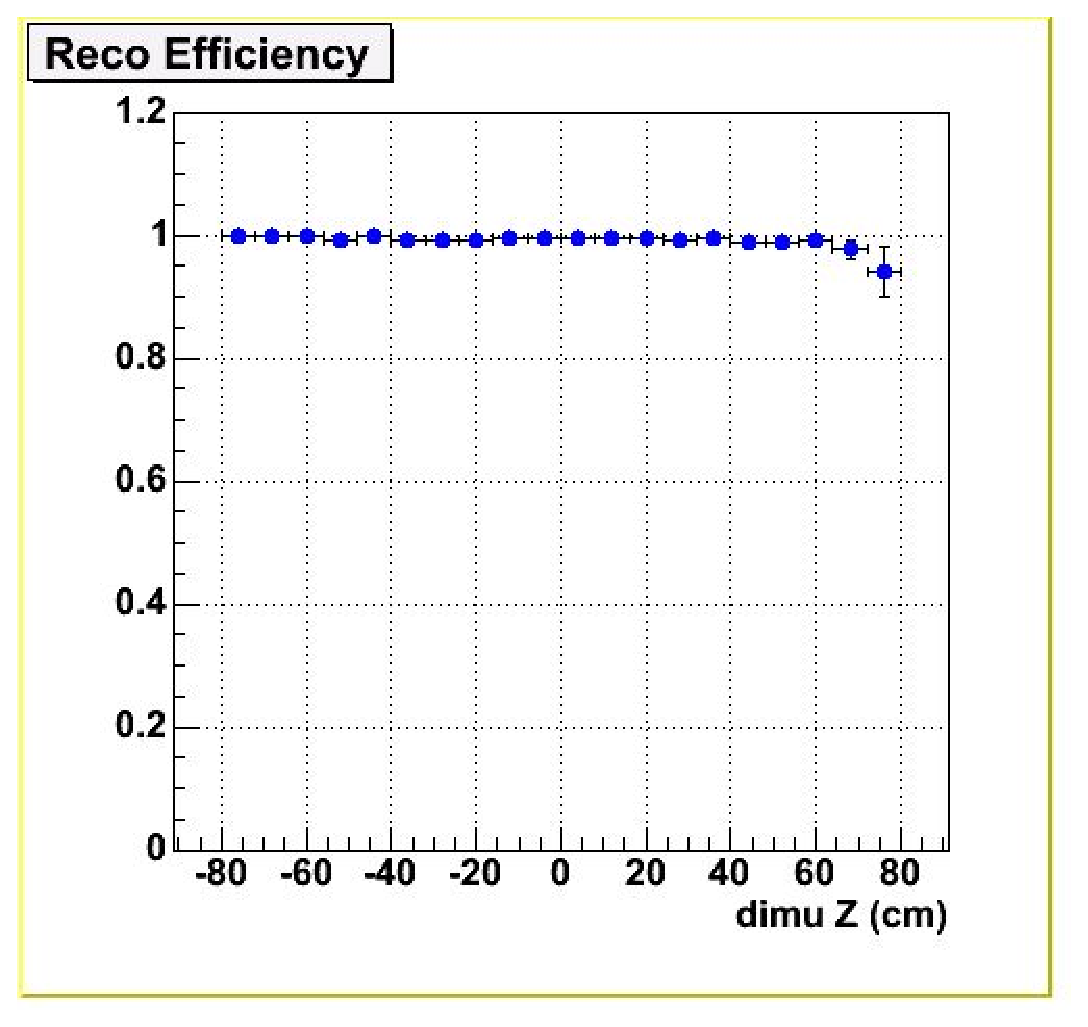
\includegraphics[width=0.65\textwidth]{eps/Reco/PV_Reco.eps}
\end{center}
\vspace{-0.1in}
\caption{Primary vertex reconstruction as measured on $Z \rightarrow ee$ data events. The efficiencies are shown as a function of the longitudinal primary vertex position~\cite{pv}.}
\label{pveff}
\end{figure}

\subsection{Jets}

Jets produced in the Monte Carlo simulation exhibit an overestimation of energy resolution, energy scale, and reconstruction efficiency. A procedure called SSR (Smearing, Shifting, and Removing) was designed to properly account for each of these relative differences between data and Monte Carlo~\cite{ssr}.

Jet energy resolution, energy scale, and reconstruction efficiency in the data and Monte Carlo are studied in back-to-back photon+jet events. In these events a variable called the transverse momentum imbalance, as shown in Eq.~\ref{deltaS}, is used to study these effects.

\begin{equation}
\label{deltaS}
\Delta S = \frac{p_{T}^{\rm{Jet}} - p_{T}^{\rm{\gamma}}}{p_{T}^{\rm{Jet}}}
\end{equation}

To determine the difference in the jet energy reconstruction efficiency in data and Monte Carlo, the $\Delta S$~distribution is determined in several regions of photon $p_{T}$ and fit to a Gaussian convoluted with a jet reconstruction efficiency function as shown in Eq.~\ref{deltaSfit}.

\begin{equation}
\label{deltaSfit}
f(\Delta S) = N \times \left( 1 + erf  \left[ \frac{\Delta S - \alpha}{\sqrt{2} \beta} \right] \right) \times \mathrm{exp} \left\{ -\frac{(\Delta S - \Delta S_{0})^{2}}{2\sigma^{2}} \right\}
\end{equation}

\noindent Where the constants $\{ \alpha, \beta \}$~characterize the jet reconstruction efficiency, $\Delta S_{0}$ yields information about the relative jet energy scale, and $\sigma$~characterizes the relative jet energy resolution.

To correct for the difference in jet energy resolution between data and Monte Carlo the Monte Carlo jet $p_{T}$ is smeared by a Gaussian with a width shown in Eq.~\ref{jetsmear}. If the generated jet $p_{T}$ is less than 15 GeV the jet is removed from the event. 
\begin{equation}
\label{jetsmear}
\sigma_{\rm{smear}} = \sqrt{ \sigma_{\rm{Data}}^{2}  - \sigma_{\rm{MC}}^{2}}
\end{equation}

The relative difference between the jet energy scale in data and Monte Carlo was found to be negligible ($\Delta S^{\rm{data}}_{0} \approx \Delta S^{\rm{MC}}_{0}$). The improved $\Delta S$ agreement between data and Monte Carlo after smearing and jet removal for two photon $p_{T}$ ranges can be seen in Fig.~\ref{jssr}.

\begin{figure}[!h!tbp]
\begin{center}
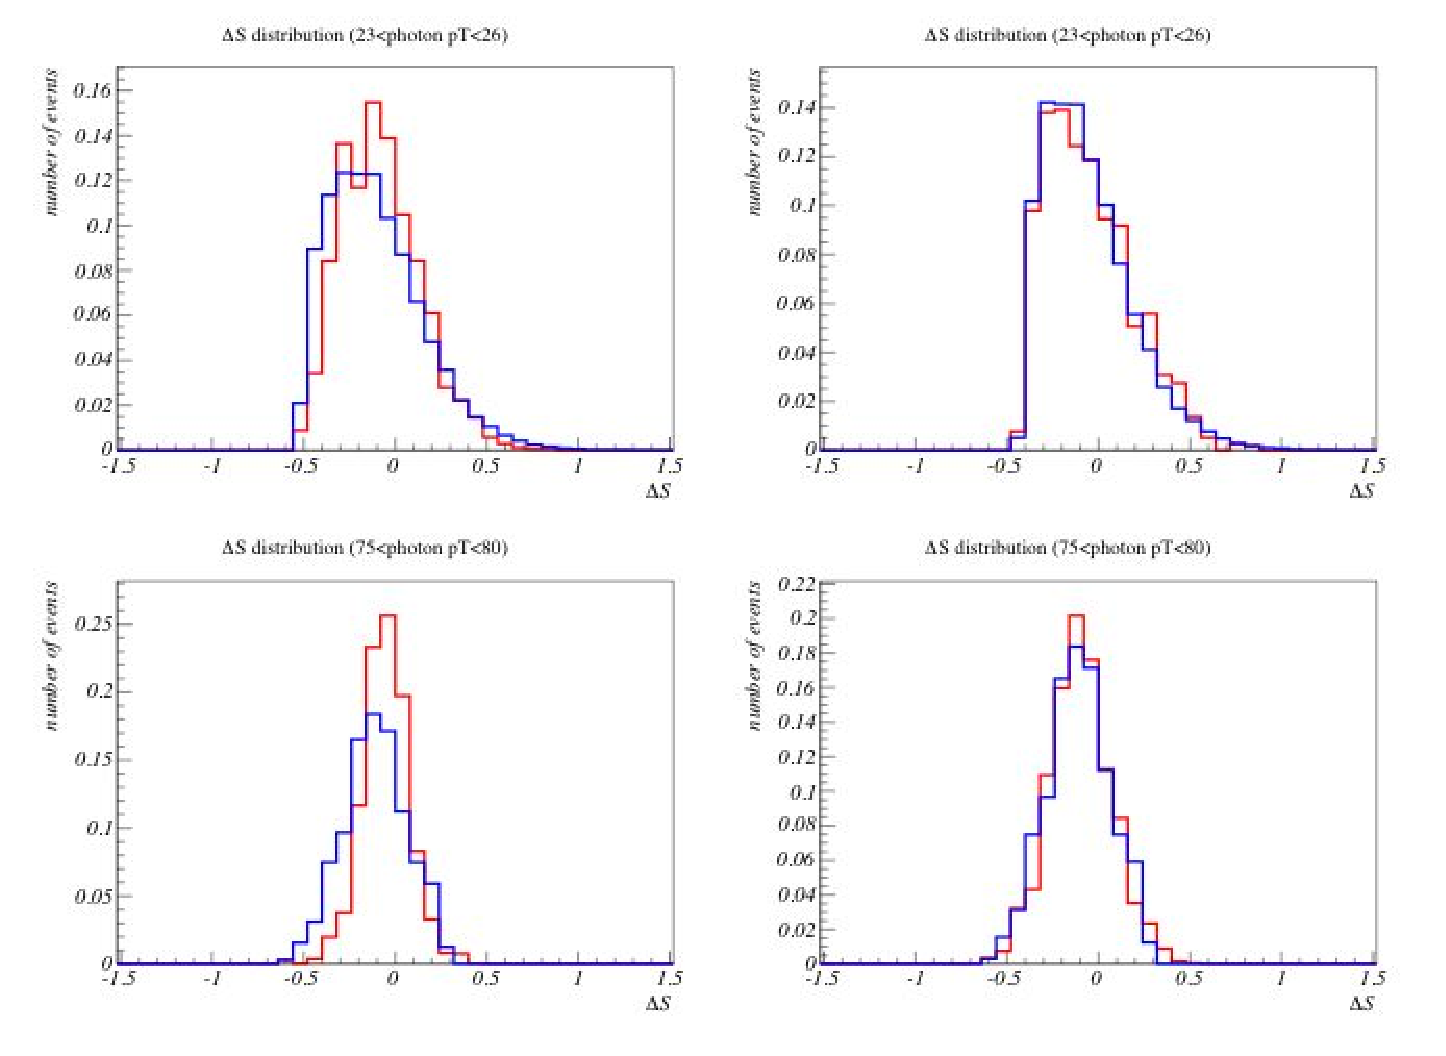
\includegraphics[width=1.0\textwidth]{eps/Reco/SSR.eps}
\end{center}
\vspace{-0.1in}
\caption{$p_{T}$ imbalance ($\Delta S$) distribution before (left) and after (right) jet smearing and removal are applied for two photon $p_{T}$ regions: $23<p_{T}^{\gamma}<26$ (top) and $75<p_{T}^{\gamma}<80$ (bottom). The data is shown in blue and the Monte Carlo is shown in red~\cite{ssr}.}
\label{jssr}
\end{figure}


\subsection{$B$-jets}

Due to large differences between data and Monte Carlo in tracking related quantities the $B$-tagging algorithms can not be directly applied to Monte Carlo events. Instead a probability for the algorithm to tag a $B$-jet, charm-jet, or a light jet is measured and applied to the Monte Carlo events~\cite{bid}. These probabilities, called tag-rate functions (TRF), are measured in data and Monte Carlo events and scaled to reproduce the expected $B$-jet, charm-jet and light-jet tagging efficiencies in data. As explained in Section~\ref{bidreco} all jets must have at least two associated tracks with $p_{T}>1$~GeV before $B$-tagging can be applied. This requirement is known as jet taggability ($\varepsilon_{\rm{Taggability}}$) and the product this quantity with the TRF yields the probability that a jet is $B$-tagged.

\begin{equation}
P_{\rm{tag}}(\vec{x}) = \varepsilon^{\rm{Taggability}}(\vec{x}) \times TRF(\vec{x})
\end{equation}

Using this per-jet tagging probability the probability that one jet is tagged in an event with $N$ jets is shown in Eq.~\ref{onetag} and probability that two jets are tagged is shown in Eq.~\ref{twotag}. These probabilities are applied to the Monte Carlo while the tagging algorithm is applied directly to the data.

\begin{equation}
\label{onetag}
P_{\rm{1-tag}} = \sum_{i=1}^{N_{\rm{jets}}} P_{\rm{tag},i} \prod_{i \neq j}^{N_{\rm{jets}}} ( 1 - P_{\rm{tag},j} )
\end{equation}

\begin{equation}
\label{twotag}
P_{\rm{2-tags}} = \sum_{i=1}^{N_{\rm{jets}}} P_{\rm{tag},i} \sum_{i \neq j}^{N_{\rm{jets}}} P_{\rm{tag},j} \prod_{k \neq i \neq j}^{N_{\rm{jets}}} ( 1 - P_{\rm{tag},k} )
\end{equation}

The $B$-jet and light-jet neural network tagging efficiencies in data are measured using a $B$-tagging algorithm that is relatively uncorrelated with the NN tagger on two different data samples. The first data sample is a relatively loose $B$-jet enriched sample requiring at least one muon with $p_{T}>4$~GeV inside a $\Delta R=0.7$ cone size jet. The presence of the muon within the jet represents a possible semi-leptonic $B$ decay. The second data sample is highly enriched in $B$-jets requiring at least two jets where one of the jets is required to have a jet impact parameter probability less than 0.5. The jet impact parameter probability is a measure of the likelihood that the jet originates from the primary interaction vertex. Large values of this quantity imply the jet originated from the hard scatter and low values indicate the jet originated from a displaced vertex. The second $B$-jet tagging algorithm used is the soft lepton tagger (SLT), which requires a muon to be reconstructed inside a jet. This algorithm is relatively uncorrelated with the NN tagger because it tags based on semi-leptonic $B$ meson decays ( e.g. $B\rightarrow D\ell\nu$ ), while the NN tagger uses information based on the displaced vertex from the $B$ decay. Using the correlation between the taggers, as measured in Monte Carlo, and the correlation between the data samples, a system of eight equations with eight unknowns can constructed. This system is then solved yielding the $B$-jet and light-jet tagging efficiencies with uncertainties in data events enriched in semi-leptonic $B$ decays.

% The $B$-jet tagging efficiency has a quite complex structure resulting from geometry of the detector and tracking inefficiencies. To avoid statistical fluctuations in the efficiency measurement, the total $B$-jet tagging efficiency is parameterized in jet $p_{T}$ and $\eta$ using the functional form shown in Eq.~\ref{btageff}.

%\begin{equation}
%\label{btageff}
%\varepsilon^{\rm{Data}}_{b\rightarrow\mu}(p_{T}, \eta) = \frac{1}{\varepsilon^{\rm{All}}} \times \left[ %\frac{c}{1+ae^{-bp_{T}}} \right] \times \left[ d + e\eta + f\eta^{2} + g\eta^{3} + h\eta^{4} \right]
%\end{equation}

The $B$-jet tagging efficiency for Monte Carlo events with a semi-leptonic $B$ decay is also measured and the ratio of the data to the Monte Carlo efficiency is used as the correction factor to the Monte Carlo. The $B$-jet tag-rate function for a Monte Carlo event with an inclusive $B$ meson decay is defined as the product of the inclusive $B$-jet tagging efficiency in Monte Carlo with the correction factor as shown in Eq.~\ref{btageff_mc}.

\begin{equation}
\label{btageff_mc}
\rm{TRF}_{b}(p_{T}, \eta) = \varepsilon_{b\rightarrow\rm{INC}}^{\rm{MC}} \times \frac{\varepsilon^{\rm{Data}}_{b\rightarrow\mu}}{\varepsilon^{\rm{MC}}_{b\rightarrow\mu}}
\end{equation}

The charm-jet tagging efficiency is measured using a similar approach with an additional input from the Monte Carlo for the relative inclusive charm-jet to $B$-jet tagging efficiency. The combined charm-jet TRF is shown in Eq.~\ref{ctageff_mc}

\begin{equation}
\label{ctageff_mc}
\rm{TRF}_{c}(p_{T}, \eta) = \varepsilon_{b\rightarrow\rm{INC}}^{\rm{MC}} \times \frac{\varepsilon^{\rm{Data}}_{b\rightarrow\mu}}{\varepsilon^{\rm{MC}}_{b\rightarrow\mu}} \times \frac{\varepsilon^{\rm{MC}}_{c\rightarrow\rm{INC}}}{\varepsilon^{\rm{MC}}_{b\rightarrow\rm{INC}}}
\end{equation}

The tag-rate functions for $B$-jets and charm-jets as a function of $p_{T}$ are shown in Fig.~\ref{bctrf}.

\begin{figure}[!h!tbp]
\begin{center}
\includegraphics[width=0.48\textwidth]{eps/Systematics/trf_b_0.775_pt.eps}
\includegraphics[width=0.48\textwidth]{eps/Systematics/trf_c_0.775_pt.eps}
\end{center}
\vspace{-0.1in}
\caption{Neural network $B$-jet tagger efficiency (green line) and $1\sigma$~error bands (dashed lines) jet $p_{T}$ and $B$-jets (left) and charm-jets (right)~\cite{bid}.}
\label{bctrf}
\end{figure}



The light-jet tagging efficiency, sometimes called the fake tag-rate (FTR), is calculated from the product of the negative tag-rate (NTR) and two Monte Carlo correction factions. The negative tag-rate is the efficiency for which a jet resulting from light flavor partons is mistaken for a $B$-jet. This typically occurs due to poor track or primary interaction vertex resolution in the event. A negative tag (NT) is found when the scalar product of the vector defined by the jet axis and the vector defined by the sum of the track vectors is negative. A positive tag is the case when the scalar product is greater than zero. Fig.~\ref{negativetag} shows the scalar products divided by the their error for $B$-jets and light jets in the Monte Carlo. 

\begin{figure}[!h!tbp]
\begin{center}
\includegraphics[width=0.65\textwidth]{eps/Reco/NegativeTag.eps}
\end{center}
\vspace{-0.1in}
\caption{The impact parameter significance for $B$-jets and light jets. The IP significance is defined as the signed scalar product of the jet-axis and vector defined by the tracks of the displaced vertex divided by the error on that measurement~\cite{aran}.}
\label{negativetag}
\end{figure}

The negative tag-rate is measured in data events with little bias towards heavy-flavor events. The NTR has two corrections which must be applied to remove any effects from heavy-flavor events that also receive a negative tag and a correction factor for the ratio of negative to positive tags for light-jets. The first correction factor is measured on $g\rightarrow b\bar{b}$ and $g\rightarrow c\bar{c}$ Monte Carlo and is defined as the ratio of the number of light-jets with a negative tag to the total number of negative tags. The second correction factor is measured on $g\rightarrow (udsg)(udsg)$ Monte Carlo and is defined as the ratio of the number of light-jets with a positive tag to the number of light-jets with a negative tag. The combined light-jet fake tag-rate function is shown in Eq.~\ref{lightjet_eff}

\begin{equation}
\label{lightjet_eff}
\rm{FTR}(p_{T}, \eta) = \rm{NTR}^{\rm{Data}} \times \frac{N^{\rm{MC}}_{l\rightarrow \rm{NT}}}{N^{\rm{MC}}_{l\rightarrow\rm{NT}} + N^{\rm{MC}}_{c\rightarrow\rm{NT}} + N^{\rm{MC}}_{b\rightarrow\rm{NT}} } \times \frac{N^{\rm{MC}}_{l\rightarrow\rm{PT}}}{N^{\rm{MC}}_{l\rightarrow\rm{NT}}}
\end{equation}

% ========== Chapter 5

\chapter{The Single Top Quark Dataset}
\label{selectioncuts}
\label{analysis}
\label{data}

This chapter describes the dataset and analysis strategy used in the search for single top quark production. This analysis is a continuation of previous single top quark searches at $\dzero$ as summarized in Section~\ref{previous}. The dataset used in the latest analysis is divided into independent samples or channels in which the single top quark analysis is performed and later combined when measuring the cross section. The division of analysis channels and the general measurement strategy is described in Section~\ref{strategy}. The triggers used to select single top-like events at runtime are described in Section~\ref{datasample}. The integrated luminosity recorded for the dataset is also reported in this section. A set of selection cuts is applied to the data set to remove mis-measured events or events which are unlikely single top quark candidates. In general the cuts are designed to select events with one high $p_{T}$ lepton from the $W$ boson decay, large missing $E_{T}$ indicating a neutrino in the final state, and two to four jets. All selection cuts are explained in Section~\ref{objectselection} with a summary table of expected fraction of $s$-channel and $t$-channel remaining after the cuts have been applied.

\section{Previous Single Top Searches}
\label{previous}

There have been several searches for single top quark production by the $\dzero$ and CDF collaborations. During Run I $\dzero$ published two analyses~\cite{Abbott:2000pa, Abazov:2001ns} using $90$~pb$^{-1}$ and set limits of $\sigma_{s-\rm{channel}} < 17$~pb and $\sigma_{t-\rm{channel}} < 22$~pb both at 95$\%$ confidence level. The CDF collaboration also published two analyses~\cite{Acosta:2004er, Acosta:2001un} using $106$~pb$^{-1}$ of Run I data resulting in limits of  $\sigma_{s-\rm{channel}} < 18$~pb and $\sigma_{t-\rm{channel}} < 13$~pb at $95\%$ confidence level.

During Run II both $\dzero$ and CDF have performed several searches for single top. $\dzero$ has published two analyses~\cite{Abazov:2005zz,Abazov:2006uq} using $230$~pb$^{-1}$ and CDF has published one analysis~\cite{Acosta:2004bs}. Both $\dzero$ and CDF have released preliminary analyses using 370 pb$^{-1}$~\cite{run2-d0-370} and 700~pb$^{-1}$~\cite{run2-cdf-bnn-700}, respectively, with improved limits.  Table~\ref{previouslimits} summarizes the limits on both $s$-channel and $t$-channel single top quark production.

\vspace{0.2in}
\begin{table}[!h!tbp]
\begin{center}
\caption{Summary of limits on $s$-channel, $t$-channel, and combined $s+t$-channel single top quark production from the $\dzero$ and CDF collaborations.}
\label{previouslimits}
\begin{tabular}{c|ccc}
%\multicolumn{4}{c}{\underline{Upper Limits on Single Top Quark Production [pb]}} \vspace{0.1in} \\
%	Analysis							&	\multicolumn{3}{c}{Production Channel} \\
Analysis									&	$s$-channel & $t$-channel & Combined $s+t$ \\
\hline
Tevatron Run I							&		&		&		\\
\hline
~~~~~~~~~~$\dzero$ with 90~pb$^{-1}$		&	17	&	22	&	-	\\
~~~~~~~~~~CDF with 106~pb$^{-1}$		&	18	&	13	&	14	\\
\hline
Tevatron Run II							&		&		&		\\
\hline
~~~~~~~~~~$\dzero$ with 162~pb$^{-1}$	&	19	&	25	&	23	\\
~~~~~~~~~~CDF with 162~pb$^{-1}$		&	13.6	&	10.1	&	17.8	\\
~~~~~~~~~~$\dzero$ with 230~pb$^{-1}$	&	6.4	&	5.0	&	-	\\
~~~~~~~~~~~~~~~~~~~~~~$\dzero$ with 370~pb$^{-1}$ (prelim.)	&	5.0	&	4.4	&	-	\\
~~~~~~~~~~~~~~~~~~~~~~CDF with 700~pb$^{-1}$ (prelim.)		&	3.2	&	2.9	&	3.4	\\
\end{tabular}
\vspace{-0.1in}
\end{center}
\end{table}

The CDF collaboration recently released three analyses using $955$~pb$^{-1}$ of Run II data. One analysis~\cite{run2-cdf-me-955} measures the combined $s$-channel and $t$-channel cross section of $2.7^{+1.5}_{-1.3}$~pb with a 2.3$\sigma$ signal significance. The other two analyses~\cite{run2-cdf-nn-955,run2-cdf-lhood-955} do not observe a significant excess of data above background and set limits on the combined $s+t$-channel production of 2.6 and 2.7~pb$^{-1}$ at 95$\%$ confidence level.

\section{Analysis Measurement Strategy}
\label{strategy}

The single top quark measurement strategy is to divide the data into many orthogonal samples, perform the analysis in each sample, and combine them during the cross section extraction procedure. The data are divided by lepton flavor, the number of reconstructed jets, and by the number of $B$-tags. The division by lepton flavor is due to the trigger selection and because events with electrons and muons suffer from different types of backgrounds. The division by the number of reconstructed jets is to ensure proper background modeling by the Monte Carlo for each jet multiplicity. Finally, the division by the number of $B$-tags is due to different sensitivities to either $s$-channel or $t$-channel events. For instance, events with one $B$-tag are sensitive to both $s$-channel and $t$-channel single top while events with two $B$-tags are only sensitive to $s$-channel events. In total there are twelve independent channels corresponding to two lepton channels (electron and muon), three reconstructed jet channels (two, three, and four), and two $B$-jet channels (one and two tags).

\section{Triggers for Single Top Quark Events}
\label{datasample}

The Run II dataset used in the single top quark analysis was collected by the $\dzero$~detector between August 2002 and December 2005. During this time there have been eight distinct periods in which the triggers used to collect data events have changed. All triggers are described in the following two sections.

\subsection{Electron Channel Trigger}
Electron channel events are selected by triggering on events with at least one electron and at least two jets~\footnote{At the trigger level an electron is still considered a jet because it deposits energy in the calorimeter in a similar way to jets.}. The electron trigger used in the single top quark analysis has changed five times during the entire run period. A description of the five triggers used is given below. Table~\ref{electrontrigger} summarizes the triggers used to collect electron single top quark events and the total integrated luminosity recorded with each trigger.

\begin{itemize}
\item $\rm{EM15\_2JT15}$
\begin{itemize}
\item Level1: One EM calorimeter tower with $E_{T}>10$~GeV and two jet calorimeter towers with $E_{T}>5$~GeV.
\item Level2: One EM object with $E_{T}>10$~GeV and electromagnetic fraction $>$~0.85. Also two jet objects with $E_{T}>10$~GeV.
\item Level3: One EM object with $E_{T}>15$~GeV and a shower shape consistent an EM object. Also, two jet objects with $E_{T}>15$~GeV.
\end{itemize}
\item $\rm{E1\_SHT15\_2J20}$
\begin{itemize}
\item Level1: One EM calorimeter tower with $E_{T}>11$~GeV.
\item Level2: No requirement.
\item Level3: One EM object with $E_{T}>15$~GeV and a shower shape consistent an EM object. Also, two jet objects with $E_{T}>20$~GeV.
\end{itemize}
\item $\rm{E1\_SHT15\_2J\_J25}$
\begin{itemize}
\item Level1: One EM calorimeter tower with $E_{T}>11$~GeV.
\item Level1: One EM object with $E_{T}>15$~GeV.
\item Level2: No requirement.
\item Level3: One EM object with $E_{T}>15$~GeV and a shower shape consistent an EM object. Also, two jet objects with $E_{T}>20$~GeV. One of the jets is also required have $E_{T}>25$~GeV.
\end{itemize}
\item $\rm{E1\_SHT15\_2J\_J30}$
\begin{itemize}
\item Level1: One EM calorimeter tower with $E_{T}>11$~GeV.
\item Level1: One EM object with $E_{T}>15$~GeV.
\item Level2: No requirement.
\item Level3: One EM object with $E_{T}>15$~GeV and a shower shape consistent an EM object. Also, two jet objects with $E_{T}>20$~GeV. One of the jets is also required have $E_{T}>30$~GeV.
\end{itemize}
\end{itemize}

\vspace{0.2in}
\begin{table}[!h!tbp]
\begin{center}
\caption{Integrated luminosities by trigger version for the triggers used to record electron single top quark events. The total integrated luminosity is shown in bold.}
\label{electrontrigger}
\begin{tabular}{cc|c}
%\multicolumn{3}{c}{\underline{Electron Triggers}}\vspace{0.1in}\\
Trigger Period	&	Trigger Name		&	Integrated Luminosity [pb$^{-1}$]	\\
\hline
I	&	E1\_SHT15\_2J15		&	103 \\ 
II	&	E1\_SHT15\_2J20		&	227 \\ 
III	&	E1\_SHT15\_2J\_J25	&	55 \\
IV	&	E1\_SHT15\_2J\_J30	&	294 \\ 
V	&	E1\_SHT15\_2J\_J25	&	234 \\
\hline
\multicolumn{2}{c|}{Total Integrated Luminosity}
                                   &  {\bf 913} \\
\end{tabular}
\vspace{-0.1 in}
\end{center}
\end{table}


\subsection{Muon Channel Trigger}

Muon channel events are selected by triggering on events with at least one muon and at least one jet. The muon trigger used in the single top quark analysis has changed seven times during the entire run period. A description of the seven triggers used is given below. Table~\ref{muontrigger} summarizes the triggers used to collect muon single top quark events and the total integrated luminosity recorded with each trigger.

\begin{itemize}
\item $\rm{MU\_JT20\_L2M0}$
\begin{itemize}
\item Level1: One muon with scintillator and wire hit and one calorimeter tower with $E_{T}>5$~GeV.
\item Level2: One muon object.
\item Level3: One jet object with $E_{T}>20$~GeV.
\end{itemize}
\item $\rm{MU\_JT25\_L2M0}$
\begin{itemize}
\item Level1: One muon with scintillator and wire hit and one calorimeter tower with $E_{T}>5$~GeV.
\item Level2: One muon object.
\item Level3: One jet object with $E_{T}>25$~GeV.
\end{itemize}
\item $\rm{MUJ2\_JT25}$
\begin{itemize}
\item Level1: One muon with scintillator and wire hit and one calorimeter tower with $E_{T}>5$~GeV.
\item Level2: One muon object and a jet object with $E_{T}>8$~GeV.
\item Level3: One jet object with $E_{T}>25$~GeV.
\end{itemize}
\item $\rm{MUJ2\_JT25\_LM3}$
\begin{itemize}
\item Level1: One muon with scintillator and wire hit and one calorimeter tower with $E_{T}>5$~GeV.
\item Level2: One muon object and a jet object with $E_{T}>8$~GeV.
\item Level3: One jet object with $E_{T}>25$~GeV and a muon object with p$_{T}>3$~GeV.
\end{itemize}
\item $\rm{MUJ2\_JT30\_LM3}$
\begin{itemize}
\item Level1: One muon with scintillator and wire hit and one calorimeter tower with $E_{T}>5$~GeV.
\item Level2: One muon object and a jet object with $E_{T}>8$~GeV.
\item Level3: One jet object with $E_{T}>30$~GeV and a muon object with p$_{T}>3$~GeV.
\end{itemize}
\item $\rm{MUJ1\_JT25\_ILM3}$
\begin{itemize}
\item Level1: One muon with scintillator and wire hit and one calorimeter tower with $E_{T}>5$~GeV.
\item Level2: One muon object and a jet object with $E_{T}>8$~GeV.
\item Level3: One jet object with $E_{T}>25$~GeV and an isolated muon object with p$_{T}>3$~GeV.
\end{itemize}
\item $\rm{MUJ1\_JT35\_LM3}$
\begin{itemize}
\item Level1: One muon with scintillator and wire hit and one calorimeter tower with $E_{T}>5$~GeV.
\item Level2: One muon object and a jet object with $E_{T}>8$~GeV.
\item Level3: One jet object with $E_{T}>35$~GeV and a muon object with p$_{T}>3$~GeV.
\end{itemize}
\end{itemize}

\vspace{0.2in}
\begin{table}[!h!tbp]
\begin{center}
\caption{Integrated luminosities by trigger version for the triggers used to record muon single top quark events. The total integrated luminosity is shown in bold.}
\label{muontrigger}
\begin{tabular}{cc|c}
%\multicolumn{3}{c}{\underline{Muon Triggers}}\vspace{0.1in}\\
Trigger Period	&	Trigger Name		&	Integrated Luminosity [pb$^{-1}$]	\\
\hline
I	&	MU\_JT20\_L2M0		&	109 \\ 
II	&	MU\_JT25\_L2M0		&	231 \\ 
III	&	MUJ2\_JT25			&	31 \\
IV	&	MUJ2\_JT25\_LM3		&	16 \\
V	&	MUJ2\_JT30\_LM3		&	252 \\
VI	&	MUJ1\_JT25\_ILM3		&	21 \\
VII	&	MUJ1\_JT35\_LM3		&	214 \\
\hline
\multicolumn{2}{c|}{Total Integrated Luminosity}
                                   &  {\bf 871} \\
\end{tabular}
\vspace{-0.1 in}
\end{center}
\end{table}


\section{Reconstructed Object Selection}
\label{objectselection}

The following sections describe the selection cuts applied to the data. The goal of the selection cuts is to remove events which are unlikely single top candidates as well as remove events which may mimic the single top quark event signature, but are created by detector noise or low energy physics processes in the event.


\subsection{Lepton Selection}

Leptons in the event must be consistent with a $W$ decay thus are required to have \mbox{$p_{T}>15 (18)$~GeV} and $|\eta|<1.1(2.0)$ for electrons (muons). To remove $Z \rightarrow \ell \ell$+jets and $\dilepton$ events a veto on additional leptons with $p_{T}>15$~GeV is applied. Events with a high $p_{T}$ muon veto event with an electron and visa versa to ensure orthogonality between search channels. Fig.~\ref{stmuon} shows the expected muon $p_{T}$ and $\eta$ distribution for $s$-channel and $t$-channel single top.

\begin{figure}[!h!tbp]
\begin{center}
\includegraphics[width=0.48\textwidth]{eps/Analysis/LeptonPt.eps}
\includegraphics[width=0.48\textwidth]{eps/Analysis/LeptonEta.eps}
\end{center}
\vspace{-0.1in}
\caption{Muon $p_{T}$ (left) and $\eta$ (right) distributions for $s$-channel (red) and $t$-channel (blue) single top. Muons are required to have $p_{T}>18$~GeV and $|\eta|<2$.}
\label{stmuon}
\end{figure}

\subsection{Jet Selection}
\label{jetselection}

Leading order $s$-channel and $t$-channel single top quark events have at most three partons in the final state which will likely yield either two or three jets. To account for higher order radiation effects events are allowed to have between two and four fully corrected jets. The leading jet (highest $p_{T}$) must have $p_{T}>25$~GeV and $|\eta^{det}|<2.5$. The second jet (second highest $p_{T}$) must have $p_{T}>20$~GeV and $|\eta^{det}|<3.4$. All other jets in the event must have $p_{T}>15$~GeV and $|\eta^{det}|<3.4$. Fig.~\ref{stjet1} shows the expected leading $p_{T}$ and $\eta$ distribution for $s$-channel and $t$-channel single top and Fig.~\ref{stjet2} shows the same distributions for the second leading jet.

\begin{figure}[!h!tbp]
\begin{center}
\includegraphics[width=0.48\textwidth]{eps/Analysis/Jet1Pt.eps}
\includegraphics[width=0.48\textwidth]{eps/Analysis/Jet1Eta.eps}
\end{center}
\vspace{-0.1in}
\caption{Leading jet $p_{T}$ (left) and $\eta$ (right) distributions for $s$-channel (red) and $t$-channel (blue) single top. The leading jet is required to have $p_{T}>25$~GeV and $|\eta|<2.5$}
\label{stjet1}
\end{figure}

\begin{figure}[!h!tbp]
\begin{center}
\includegraphics[width=0.48\textwidth]{eps/Analysis/Jet2Pt.eps}
\includegraphics[width=0.48\textwidth]{eps/Analysis/Jet2Eta.eps}
\end{center}
\vspace{-0.1in}
\caption{Second leading jet $p_{T}$ (left) and $\eta$ (right) distributions for $s$-channel (red) and $t$-channel (blue) single top. The second leading jet is required to have $p_{T}>20$~GeV and $|\eta|<3.4$}
\label{stjet2}
\end{figure}


\subsection{Missing $E_{T}$}
\label{missingetselection}

A large amount of missing transverse energy in an event can indicate the presence of a neutrino in the final state. All events are required to have M$E_{T} > 15$~GeV. Fig.~\ref{stmet} shows the missing $E_{T}$ distribution for $s$-channel and $t$-channel single top.

\begin{figure}[!h!tbp]
\begin{center}
\includegraphics[width=0.48\textwidth]{eps/Analysis/MissingEt.eps}
\end{center}
\vspace{-0.1in}
\caption{Missing $E_{T}$ distribution for $s$-channel (red) and $t$-channel (blue) single top. The missing $E_{T}$ is required to larger than 15~GeV.}
\label{stmet}
\end{figure}

\subsection{Vertex Selection}
\label{vertexselection}

All events are required to have one and only one primary interaction vertex as defined in Section~\ref{pvreco}. No requirement is placed on additional minimum bias vertices in the event. Fig.~\ref{stpv} shows the primary interaction vertex longitudinal location distribution for $s$-channel and $t$-channel single top.

\begin{figure}[!h!tbp]
\begin{center}
\includegraphics[width=0.48\textwidth]{eps/Analysis/PVz.eps}
\end{center}
\vspace{-0.1in}
\caption{Longitudinal location of the primary interaction vertex for $s$-channel (red) and $t$-channel (blue) single top. The primary interaction vertex is required to be located within 60~cm of the detector origin.}
\label{stpv}
\end{figure}

\subsection{b-Jet Selection}
\label{bjetselection}

Both $s$-channel and $t$-channel single top quark events have at least one b quark in the final state thus all events are required to have at least one $B$-tagged jet as identified by the neural network tagging algorithm.

\subsection{Mis-measured event rejection}
\label{misidselection}

There are several selection cuts applied to reduce mis-measured events. First, all events are required to have less than $200$~GeV of missing $E_{T}$. This cut is applied to remove events where the muon track momentum has been badly measured, which can cause a large imbalance in the missing transverse energy measurement. All events are also allowed at most three ``noise" jets. A noise jet is a jet that fails one of the criteria specified in Section~\ref{jetreco} and is not matched to an electromagnetic cluster. It has been observed that allowing more than three noise jets alters the $p_{T}$ and $\eta$~distributions of other jets in the event. The final set of cuts applied to remove unwanted events are ``triangle cuts", which are cuts between the difference in $\phi$ between an object and the missing $E_{T}$ versus the missing $E_{T}$. An example of triangle cut is shown in Fig.~\ref{triangleexample}. Three sets of triangle cuts are applied to the data and Monte Carlo events and shown in the bullets below.

\begin{itemize}
\item Electron Triangle Cuts: $|\Delta\phi(\rm{e},ME_{T})|$~vs.~$\met$
   \begin{itemize}
   \item $0<|\Delta\phi|<2$~ when $ME_{T} = 0$~GeV, and $0<ME_{T}<40$~GeV when $|\Delta\phi| = 0$
   \item $0<|\Delta\phi|<1.5$~ when $ME_{T} = 0$~GeV, and $0<ME_{T}<50$~GeV when $|\Delta\phi| = 0$
   \item  $2<|\Delta\phi|<\pi$~ when $ME_{T} = 0$~GeV, and $0<ME_{T}<24$~GeV when $|\Delta\phi| = \pi$
   \end{itemize}
\item Muon Triangle Cuts: $|\Delta\phi(\mu,ME_{T})|$~vs.~$\met$
   \begin{itemize}
   \item  $0<|\Delta\phi|<1.1$~ when $ME_{T} = 0$~GeV, and $0<ME_{T}<80$~GeV when $|\Delta\phi| = 0$
   \item  $0<|\Delta\phi|<1.5$~ when $ME_{T} = 0$~GeV, and $0<ME_{T}<50$~GeV when $|\Delta\phi| = 0$
   \item $2.5<|\Delta\phi|<\pi$~ when $ME_{T} = 0$~GeV, and $0<ME_{T}<30$~GeV when $|\Delta\phi| = \pi$
   \end{itemize}
\item Leading Jet Triangle Cut: $|\Delta\phi(\rm{Jet_{1}},ME_{T})|$~vs.~$\met$
   \begin{itemize}
   \item $1.5<|\Delta\phi|<\pi$~ when $ME_{T} = 0$~GeV, and $0<ME_{T}<35$~GeV when $|\Delta\phi| = \pi$
   \end{itemize}
\end{itemize}



\begin{figure}[!h!tbp]
\begin{center}
\includegraphics[width=0.48\textwidth]{eps/Reco/TriangleExample.eps}
\includegraphics[width=0.48\textwidth]{eps/Reco/TriangleExampleSignal.eps}
\end{center}
\vspace{-0.1in}
\caption{Example triangle cut between a muon and the missing $E_{T}$ for mis-measured events (left) and $s$-channel single top events (right). The colors indicate the density of events. The brighter colors indicate more densely populated regions. Events which fall inside the triangles are removed from the final data sample. The black line at M$E_{T}=15$~GeV indicates the standard missing $E_{T}$ selection~\cite{oldsingletopnote}.} 
\label{triangleexample}
\end{figure}

\subsection{Acceptance for Single Top Quark Events}
\label{acceptance}

The signal acceptance is defined as:

\begin{equation}
\mathcal{A} = \frac{1}{\rm{N}_{\rm initial}}
\sum_{i}^{\rm{N}_{\rm selected}} \left[ \varepsilon_{\rm trigger} \times
\varepsilon_{\rm corrections} \times \varepsilon_{\rm TRF} \right]
\end{equation}

\noindent where $\rm{N}_{\rm initial}$ is the initial
number of events in each MC sample, $\rm{N}_{\rm selected}$ is the number of MC events
remaining after selection, $\varepsilon_{\rm{trigger}}$ is the trigger weight, $\varepsilon_{\rm{corrections}}$ are the Monte Carlo correction factors, and $\varepsilon_{\rm{TRF}}$ is the $B$-tagging weight. Table~\ref{acceptances} shows the percentage of each single top quark
signal for each jet multiplicity that remain after selection cuts.


\vspace{0.2in}
\begin{table}[!h!tbp]
\begin{center}
\caption{Single acceptances after selection cuts, one, and two $B$-tags. The branching ratio for $W\rightarrow \ell\nu$~is included in the acceptance.}
\label{acceptances}
\begin{tabular}{c|ccc|ccc}
%\multicolumn{7}{c}{\hspace{1in}\underline{$s$-channel and $t$-channel Signal Acceptances}}\vspace{0.1in} \\
& \multicolumn{3}{c|}{Electron Channel} & \multicolumn{3}{c}{Muon Channel} \\
                     & 2 jets & 3 jets & 4 jets
                     & 2 jets & 3 jets & 4 jets \\
\hline
Before $B$ tagging	&        	&        	&        	&        	&        	&        	\\
~~$tb$               		& 1.77\%	& 0.83\% 	& 0.23\%	& 1.36\% 	& 0.69\% 	& 0.19\%	\\
~~$tqb$              	& 1.49\% 	& 0.79\% 	& 0.25\% 	& 1.17\% 	& 0.64\% 	& 0.20\%	\\
\hline
One $B$-tagged jet   &        	&        	&        	&        	&        	&        	\\
~~$tb$               		& 0.82\% 	& 0.39\% 	& 0.11\% 	& 0.64\% 	& 0.32\% 	& 0.09\%	\\
~~$tqb$              	& 0.61\% 	& 0.34\% 	& 0.11\% 	& 0.50\% 	& 0.28\% 	& 0.09\%	\\
\hline
Two $B$-tagged jets	&        	&        	&        	&        	&        	&        	\\
~~$tb$               		& 0.29\% 	& 0.14\% 	& 0.04\% 	& 0.24\% 	& 0.12\% 	& 0.03\%	\\
~~$tqb$              	& 0.02\% 	& 0.05\% 	& 0.02\% 	& 0.01\% 	& 0.04\% 	& 0.02\%
\end{tabular}
\vspace{-0.1in}
\end{center}
\end{table} 

% ========== Chapter 6

\chapter{Background Estimation}
\label{background}
\label{backgrounds}

Perhaps the most critical aspect of a physics analysis is estimating the background contribution in the data sample. Most physics backgrounds can be modeled using simulated Monte Carlo events and the rest are modeled using reconstructed data events. This chapter describes how all backgrounds are modeled and normalized to their expected contribution in the dataset. Section~\ref{backgroundmodel} describes the expected backgrounds in the single top quark dataset and how the background event kinematics are modeled. Section~\ref{backgroundnorm} describes how these backgrounds are normalized to their expected yields in the dataset. Finally, Section~\ref{backgroundyields} summarizes all background yields and Section~\ref{databackcompare}~compares data with the expected background estimation.

\section{Background Modeling}
\label{backgroundmodel}

As described in Chapter~\ref{theory} the top quark in single top quark events will decay to a $W$ boson and $b$ quark, where the $W$ boson is only considered to decay to a lepton and neutrino in this analysis\footnote{$t\rightarrow bW \rightarrow bqq^{'}$ decays are removed from the dataset since there is no lepton nor large missing $E_{T}$.}. With an additional $b$ quark or light quark this makes the signature of single top quark events one high $p_{T}$ lepton, large missing $E_{T}$, and two or more jets. This event signature can be produced by three general types of backgrounds. The largest background which produces this event signature is $W$ or $Z$ boson production in association with two or more jets. Because the kinematics of $Z$ boson production are similar to $W$ boson production, both backgrounds are typically considered as one background called ``$W$+jets". An example Feynman diagram for such a process is shown in Fig.~\ref{wjetsexample}.

\begin{figure}[!h!tbp]
\begin{center}
\includegraphics[width=0.5\textwidth]{eps/Feynman/feynman_Wbbg.eps}
\end{center}
\vspace{-0.1in}
\caption{Example leading order Feynman diagram for a ``$W$+jets" event. This particular diagram represents the production of a $W$ boson, and two $b$~quarks and an associated gluon~\cite{feynmandiagrams}.}
\label{wjetsexample}
\end{figure}

Another large background present in the dataset are events origination from top pair production. The top pair production background, referred to as $\ttbar$, is defined by the decay of the two $W$ bosons, from the decay of the two top quarks. The first case when one of the $W$ bosons decays to two quarks and other decays to a lepton and neutrino is referred to as ``lepton+jets" ($\lepjets$) because the final state in the event is one lepton, one neutrino, and four quarks. The other way in which a $\ttbar$~event can enter the data sample is when both $W$ bosons decay to leptons and neutrinos. In this case, there are two quarks, two leptons, and two neutrinos. These events are referred to as ``dilepton'' ($\dilepton$) events. An example Feynman diagram for the $\lepjets$~process is shown in Fig.~\ref{ttbarexample}.

\begin{figure}[!h!tbp]
\begin{center}
\includegraphics[width=0.5\textwidth]{eps/Feynman/feynman_ttbar_ljets.eps}
\end{center}
\vspace{-0.1in}
\caption{Example Feynman diagram for a $\lepjets$ event~\cite{feynmandiagrams}.}
\label{ttbarexample}
\end{figure}

The third largest background present in the dataset is multijet events produced by the strong interaction. The background processes responsible for these events in the dataset are quite different for electron events and muon events. In electron events one of the reconstructed jets will have a large electromagnetic fraction causing it to be mis-identified as an electron. In muon events a gluon will decay to a $b\bar{b}$ pair and one of the $B$ mesons will undergo a semi-leptonic decay and produce a muon. In both cases, another jet may not be properly reconstructed leading to a large amount of missing E$_{T}$ in the event, thus mimicking the single top quark event signature. An example Feynman diagram for a multijet process producing a lepton, missing E$_{T}$, and jets is shown in Fig.~\ref{qcdexample}.

\begin{figure}[!h!tbp]
\begin{center}
\includegraphics[width=0.5\textwidth]{eps/Feynman/feynman_bbbar_ljets.eps}
\end{center}
\vspace{-0.1in}
\caption{Example Feynman diagram for a multijet event~\cite{feynmandiagrams}.}
\label{qcdexample}
\end{figure}


\subsection{Monte Carlo Modeling of W + Jets and $\ttbar$ Backgrounds}
\label{wjetsmodel}
$W$+jets and $\ttbar$ backgrounds are modeled using the ALPGEN Monte Carlo generator interfaced with Pythia for parton showering~\cite{Mangano:2002ea}. ALPGEN is a leading order matrix element Monte Carlo generator similar to the CompHEP generator used to model single top quark events. All generated events are reconstructed using the simulated $\dzero$~detector as described in Chapter~\ref{EventSelection} and selection cuts are applied as described in Chapter~\ref{analysis}. Within ALPGEN, the MLM jet-parton matching scheme~\cite{Hoche:2006ph} is also employed to remove double counted events in a similar manner to the double counting that is encountered when generating single top events. An example of double counting in $W$+jets events is given here: $W$+light flavor events (e.g $Wgg$) are generated separately from $W$+heavy flavor events (e.g $Wbb$). When these events are sent through Pythia it is possible that addition gluons will split to heavy flavor quarks (e.g $g\rightarrow b\bar{b}$) leading to double counting of $W$+heavy flavor events. The MLM matching scheme is described in more detail below.

\subsubsection{MLM Matching Scheme}

As stated earlier, the MLM jet-parton matching scheme is designed to remove double counted events. The MLM matching scheme works in the following way:

\begin{enumerate}
\item Events are generated with a distinct parton multiplicity. For instance, $W$+2 light partons (e.g. $Wgg$) are generated separately from $W$+3 light partons (e.g. $Wggg$). The same applies to $W$+heavy flavor and $\ttbar$~events.
\item All generated events are sent to Pythia for parton showering. This procedure will introduce additional quarks and gluons as a product of the shower.
\item Before the final state partons are hadronized, all quarks and gluons are clustered together with a jet algorithm. The algorithm used for this analysis is the UA1 jet cone algorithm~\cite{PhysRevLett.54.1983}.
\item Match the generated partons from (1) with the cone jets from (3). Each parton must correspond to one jet and visa versa. A jet is matched if it has p$_{T}>15$~GeV and there is a parton with $\Delta R<0.7$ from the jet. If a match is found the event is kept, otherwise the process is repeated.
\item Combine all samples together with weights based on the relative cross sections and the relative number of generated events for each process. 
\end{enumerate}

The formulas used to combined $W$+light parton, $W$+$c\bar{c}$+light parton, $W$+$b\bar{b}$+light parton, $\dilepton$+light parton, and $\lepjets$+light parton events are shown below.

\subsubsection{$W$+Light Parton Sample}

The $W$+light parton sample contains $W$+light flavor ($udsg$) events as well as $W$+$c$+light flavor events. In $W$+$c$+light flavor events the $c$-quark is considered massless. Eq.~\ref{wlp} shows the formula used to combine the $W$+light parton sample and Table~\ref{wjjcross} shows the relative cross sections and weights (k) for each sample. All $W$+light parton events are generated using CTEQ6L1 PDFs with $Q^{2}=m_{W}^{2} + P^{2}_{T}(W)$.

\begin{eqnarray}
\label{wlp}
\nonumber
W+\rm{Nlp} &=& k_{W+0\rm{lp}} \left[W+0\rm{lp}\right]_{\rm{excl}} + k_{W+1\rm{lp}} \left[W+1\rm{lp}\right]_{\rm{excl}} + \\
\nonumber
& & k_{W+2\rm{lp}} \left[W+2\rm{lp}\right]_{\rm{excl}} + k_{W+3\rm{lp}} \left[W+3\rm{lp}\right]_{\rm{excl}} + \\
& & k_{W+4\rm{lp}} \left[W+4\rm{lp}\right]_{\rm{excl}} + k_{W+5\rm{lp}} \left[W+5\rm{lp}\right]_{\rm{incl}}	\\
\nonumber
\end{eqnarray}



\begin{table}[!h!tbp]
\begin{center}
\caption{Absolute weights for $W$+light parton ALPGEN Monte Carlo events.}
\label{wjjcross}
\begin{tabular}{c|cccc}
%\multicolumn{5}{c}
%{\underline{Absolute Weights For $W$+Light Parton ALPGEN Monte Carlo Events}} \\
Sample			&	Type		&	Cross Section [pb]	&	Events	&	Weight (k) \\
\hline
$k_{W+0\rm{lp}}$	&	Exclusive	&	$4574$			&	7844750	&	$2.15$			\\
$k_{W+1\rm{lp}}$	&	Exclusive	&	$1273$			&	1053000	&	$0.68$			\\
$k_{W+2\rm{lp}}$	&	Exclusive	&	$298.5$			&	1250500	&	$0.34$	\\
$k_{W+3\rm{lp}}$	&	Exclusive	&	$70.56$			&	621000	&	$16.4$	\\
$k_{W+4\rm{lp}}$	&	Exclusive	&	$15.83$			&	582250	&	$0.07$	\\
$k_{W+5\rm{lp}}$	&	Inclusive	&	$11.29$			&	41750	&	$0.13$
\end{tabular}
\vspace{-0.1 in}
\end{center}
\end{table}

\subsubsection{$W$+$c\bar{c}$+Light Parton Sample}

The $W$+$c\bar{c}$+light parton sample contains $W$+$c\bar{c}$ (from gluon splitting) + light flavor partons. In contrast to the $W$+light parton samples the $c$-quark in these events are massive. Eq.~\ref{wcc} shows the formula used to combine the $W$+$c\bar{c}$+light parton sample and Table~\ref{wcccross} shows the relative cross sections and weights (k) for each sample. All $W$+$c\bar{c}$+light parton events are generated using CTEQ6L1 PDFs with $Q^{2}=m_{W}^{2} + P^{2}_{T}(W)$.

\begin{eqnarray}
\label{wcc}
\nonumber
W+c\bar{c}+\rm{Nlp} &=& k_{W+c\bar{c}+0\rm{lp}} \left[W+c\bar{c}+0\rm{lp}\right]_{\rm{excl}} + k_{W+c\bar{c}+1\rm{lp}} \left[W+c\bar{c}+1\rm{lp}\right]_{\rm{excl}} + \\
& & k_{W+c\bar{c}+2\rm{lp}} \left[W+c\bar{c}+2\rm{lp}\right]_{\rm{excl}} + k_{W+c\bar{c}+3\rm{lp}} \left[W+c\bar{c}+3\rm{lp}\right]_{\rm{incl}}
\end{eqnarray}


\begin{table}[!h!tbp]
\begin{center}
\caption{Absolute weights for $W$+$c\bar{c}$+light parton ALPGEN Monte Carlo events.}
\label{wcccross}
\begin{tabular}{c|cccc}
%\multicolumn{5}{c}
%{\underline{Absolute Weights For $W$+$c\bar{c}$+Light Parton ALPGEN Monte Carlo Events}} \\
Sample					&	Type		&	Cross Section [pb]	&	Events	&	Weight (k) \\
\hline
$k_{W+c\bar{c}+0\rm{lp}}$	&	Exclusive	&	$71.15$			&	481572	&	$0.039$			\\
$k_{W+c\bar{c}+1\rm{lp}}$	&	Exclusive	&	$29.85$			&	336400	&	$0.036$			\\
$k_{W+c\bar{c}+2\rm{lp}}$	&	Exclusive	&	$10.25$			&	332347	&	$0.016$	\\
$k_{W+c\bar{c}+3\rm{lp}}$	&	Inclusive	&	$18.39$			&	372248	&	$0.020$	\\
\end{tabular}
\vspace{-0.1 in}
\end{center}
\end{table}

\subsubsection{$W$+$b\bar{b}$+Light Parton Sample}

The $W$+$b\bar{b}$+light parton sample contains $W$+$b\bar{b}$ (from gluon splitting) + light flavor partons. Eq.~\ref{wjetsbbsample} shows the formula used to combine the $W$+$b\bar{b}$+light parton sample and Table~\ref{wbbcross} shows the relative cross sections and weights (k) for each sample. All $W$+$b\bar{b}$+light parton events are generated using CTEQ6L1 PDFs with $Q^{2}=m_{W}^{2} + P^{2}_{T}(W)$.


\begin{eqnarray}
\label{wjetsbbsample}
\nonumber
W+b\bar{b}+\rm{Nlp} &=& k_{W+b\bar{b}+0\rm{lp}} \left[W+b\bar{b}+0\rm{lp}\right]_{\rm{exbl}} + k_{W+b\bar{b}+1\rm{lp}} \left[W+b\bar{b}+1\rm{lp}\right]_{\rm{exbl}} + \\
& & k_{W+b\bar{b}+2\rm{lp}} \left[W+b\bar{b}+2\rm{lp}\right]_{\rm{exbl}} + k_{W+b\bar{b}+3\rm{lp}} \left[W+b\bar{b}+3\rm{lp}\right]_{\rm{incl}}
\end{eqnarray}

\begin{table}[!h!tbp]
\begin{center}
\caption{Absolute weights for $W$+$b\bar{b}$+light parton ALPGEN Monte Carlo events.}
\label{wbbcross}
\begin{tabular}{c|cccc}
%\multicolumn{5}{c}
%{\underline{Absolute Weights For $W$+$b\bar{b}$+Light Parton ALPGEN Monte Carlo Events}} \\
Sample					&	Type		&	Cross Section [pb]	&	Events	&	Weight (k) \\
\hline
$k_{W+b\bar{b}+0\rm{lp}}$	&	Exclusive	&	$19.18$			&	738761	&	$0.014$			\\
$k_{W+b\bar{b}+1\rm{lp}}$	&	Exclusive	&	$7.939$			&	261300	&	$0.011$			\\
$k_{W+b\bar{b}+2\rm{lp}}$	&	Exclusive	&	$2.636$			&	171411	&	$0.005$	\\
$k_{W+b\bar{b}+3\rm{lp}}$	&	Inclusive	&	$1.742$			&	163674	&	$0.003$	\\
\end{tabular}
\vspace{-0.1 in}
\end{center}
\end{table}



\subsubsection{$\lepjets$+Light Parton Sample}

The $\lepjets$+light parton sample contains $\lepjets$ + light flavor partons. Eq.~\ref{ttbarsample} shows the formula used to combine the $\lepjets$+light parton sample and Table~\ref{lepjetscross} shows the relative cross sections and weights (k) for each sample. All $\lepjets$ events are generated using CTEQ6L1 PDFs with scale $Q^{2}=m_{t}^{2} + \sum_{\rm{jets}}P^{2}_{T}$.

\begin{eqnarray}
\label{ttbarsample}
\nonumber
\lepjets+Nlp&=& k_{\lepjets+0\rm{lp}} \left[\lepjets+0\rm{lp}\right]_{\rm{excl}} +\\
\nonumber
& & k_{\lepjets+1\rm{lp}} \left[\lepjets+1\rm{lp}\right]_{\rm{excl}} + \\
& & k_{\lepjets+2\rm{lp}} \left[\lepjets+2\rm{lp}\right]_{\rm{incl}} 
\end{eqnarray}


\begin{table}[!h!tbp]
\begin{center}
\caption{Absolute weights for $\lepjets$+light parton ALPGEN Monte Carlo events.}
\label{lepjetscross}
\begin{tabular}{c|cccc}
%\multicolumn{5}{c}
%{\underline{Absolute Weights For $\lepjets$+Light Parton ALPGEN Monte Carlo Events}} \\
Sample				&	Type		&	Cross Section [pb]	&	Events	&	Weight (k) \\
\hline
$k_{\lepjets+0\rm{lp}}$	&	Exclusive	&	$1.284$			&	283463	&	$0.048$			\\
$k_{\lepjets+1\rm{lp}}$	&	Exclusive	&	$0.625$			&	98425	&	$0.032$			\\
$k_{\lepjets+2\rm{lp}}$	&	Inclusive	&	$0.398$			&	92517	&	$0.020$			\\
\end{tabular}
\vspace{-0.1 in}
\end{center}
\end{table}



\subsubsection{$\dilepton$+Light Parton Sample}

The $\dilepton$+light parton sample contains $\dilepton$ + light flavor partons. Eq.~\ref{ttbardilepsample} shows the formula used to combine the $\dilepton$+light parton sample and Table~\ref{dileptoncross} shows the relative cross sections and weights (k) for each sample. All $\dilepton$ events are generated using CTEQ6L1 PDFs with scale $Q^{2}=m_{t}^{2} + \sum_{\rm{jets}}P^{2}_{T}$.

\begin{eqnarray}
\label{ttbardilepsample}
\nonumber
\dilepton+Nlp&=& k_{\dilepton+0\rm{lp}} \left[\dilepton+0\rm{lp}\right]_{\rm{excl}} +\\
\nonumber
& & k_{\dilepton+1\rm{lp}} \left[\dilepton+1\rm{lp}\right]_{\rm{excl}} + \\
& & k_{\dilepton+2\rm{lp}} \left[\dilepton+2\rm{lp}\right]_{\rm{incl}} 
\end{eqnarray}


\begin{table}[!h!tbp]
\begin{center}
\caption{Absolute weights for $\dilepton$+light parton ALPGEN Monte Carlo events.}
\label{dileptoncross}
\begin{tabular}{c|cccc}
%\multicolumn{5}{c}
%{\underline{Absolute Weights For $\dilepton$+Light Parton ALPGEN Monte Carlo Events}} \\
Sample				&	Type		&	Cross Section [pb]	&	Events	&	Weight (k) \\
\hline
$k_{\dilepton+0\rm{lp}}$	&	Exclusive	&	$0.324$			&	223635	&	$0.0004$			\\
$k_{\dilepton+1\rm{lp}}$	&	Exclusive	&	$0.151$			&	96386	&	$0.0078$			\\
$k_{\dilepton+2\rm{lp}}$	&	Inclusive	&	$0.104$			&	148105	&	$0.0051$			\\
\end{tabular}
\vspace{-0.1 in}
\end{center}
\end{table}



\subsection{Data-based Modeling of Multijet Background}

In both electron and muon samples the multijet background is a result of muons from heavy flavor decays or jets with a large electromagnetic fraction mimicking a lepton from a $W$ boson decay. The multijet background is modeled using data events that pass all selection cuts except the isolation cut for muons or likelihood cut for electrons. The normalization of this background as well as all Monte Carlo modeled backgrounds is described in Section~\ref{backgroundnorm}

\section{Background Normalization}
\label{backgroundnorm}

\subsection{\ttbar~Normalization}
\label{ttbarnormmethod}

All $\ttbar$ Monte Carlo events are normalized to the number of events expected from the NLLO $\ttbar$~cross section and branching ratio multiplied by the integrated luminosity as shown in Eq.~\ref{ttbarnorm}.

\begin{equation}
\label{ttbarnorm}
N_{\ttbar} = \sigma_{\ttbar} \times \rm{BR} \times \int \mathcal{L}\rm{dt}
\end{equation}

The cross sections shown in Tables~\ref{lepjetscross} and~\ref{dileptoncross} are leading order cross sections from ALPGEN that must be scaled to match the next-to-next-leading log cross section of $6.67$~pb as calculated in~\cite{Kidonakis:2003vs,cacciari-2004-0404}. Each event is then assigned a weight such that the total number of weighted Monte Carlo events equals $N_{\ttbar}$. The event weight is shown in Eq.~\ref{ttbarweight}.

\begin{equation}
\label{ttbarweight}
w_{i} = \frac{N_{\ttbar}}{\sum_{i}^{\rm{N}_{\rm selected}} \left[ \varepsilon_{\rm trigger} \times
\varepsilon_{\rm corrections} \times \varepsilon_{\rm TRF} \right]}
\end{equation}

\subsection{Matrix Method: Normalizing $W$+jets and Multijet Backgrounds}

The $W$+jets and multijet backgrounds are normalized through a procedure known as the matrix method. This method requires two datasets to determine the mixture of $W$+jets and multijet backgrounds. The first sample contains a mixture of $W$+jets and multijet events while the second sample is enriched in $W$+jets. The sample that contains the mixture of events is called the ``loose" sample and is defined in Eq.~\ref{loosedef} and a subset of that sample which is enriched in $W$ decays and is called the ``tight" sample and is defined in Eq.~\ref{tightdef}. In both samples the $\ttbar$~background is normalized as described in Section~\ref{ttbarnormmethod}. The tight sample is a subset of the loose sample with the only difference being that tight events have passed the muon isolation selection cut or the electron likelihood cut.

\begin{eqnarray}
\label{loosedef}
\rm{N}_{\rm{loose}} &=& \rm{N}_{\rm{Multijet}} +  \rm{N}_{\rm{W+jets}} + \rm{N}_{\ttbar}	\\
\label{tightdef}
\rm{N}_{\rm{tight}} &=& \varepsilon_{\rm{Multijet}} \times \rm{N}_{\rm{Multijet}} + \varepsilon_{\rm{W+jets}} \times \left[ \rm{N}_{\rm{W+jets}} + \rm{N}_{\ttbar} \right]
\end{eqnarray}

The two parameters, $\varepsilon_{\rm{Multijet}}$ and $\varepsilon_{\rm{W+jets}}$, represent the efficiency with which multijet and $W$+jets events satisfy the tight selection requirement given the loose selection  requirement. By inverting the system of two equations and by measuring the two $\varepsilon$~parameters, the expected number of $W$+jets and multijet events can be determined. The formula for the expected number of $W$+jets events is shown in Eq.~\ref{wjetssolution} and the formula for the expected number of multijet events is shown in Eq.~\ref{qcdsolution}. The methods used to measure the efficiency parameters are shown in the appropriately labeled sections below. The number of loose and tight events for each jet multiplicity is shown in Table~\ref{nloosentight} along with the expected number of multijet and $W$+jets events in the tight sample.

\begin{equation}
\label{wjetssolution}
\rm{N}_{\rm{W+jets}} = \frac{\rm{N}_{\rm{tight}} - \varepsilon_{\rm{Multijet}} \times \rm{N}_{\rm{loose}}}{\varepsilon_{\rm{W+jets}}  - \varepsilon_{\rm{Multijet}}} - \rm{N}_{\ttbar}
\end{equation}

\begin{equation}
\label{qcdsolution}
\rm{N}_{\rm{Multijet}} = \frac{\rm{\varepsilon_{\rm{W+jets}} \times \rm{N}_{\rm{loose}} - N}_{\rm{tight}}}{\varepsilon_{\rm{W+jets}}  - \varepsilon_{\rm{Multijet}}}
\end{equation}


\vspace{0.2in}
\begin{table}[!h!tbp]
\begin{center}
\caption{Number of loose and tight data events after all selection cuts (top two rows) along with the expected number $W$+jets and multijet events in the tight sample (bottom two rows).}
\label{nloosentight}
\begin{tabular}{c|ccc|ccc}
%\multicolumn{7}{c}{\hspace{1in}\underline{Expected Yields From The Matrix Method}}\vspace{0.1in} \\
& \multicolumn{3}{c|}{Electron Channel} & \multicolumn{3}{c}{Muon Channel}    \\
                               & 2 jets & 3 jets & 4 jets
                               & 2 jets & 3 jets & 4 jets \\
\hline
N$_{{\rm loose}}$              	& 15,213 &  7,118 &  2,191 &   7,092 &  3,054 &   878	\\
N$_{{\rm tight}}$              	& 8,220 &  3,075 &    874 &   6,432 &  2,590 &   727		\\
$\varepsilon_{\rm{Multijet}}\times$N$_{\rm{Multijet}}$	& 1,433 &    860 &    256 &    329 &    223 &    56	\\
$\varepsilon_{\rm{W+jets}}\times$N$_{\rm{W+jets}}$		& 6,787 &  2,215 &    618 &   6,105 &  2,369 &   669
\end{tabular}
\vspace{-0.1in}
\end{center}
\end{table}


All $W$+jets events are then given a weight such that the total number of weighted events equals the expected yields shown in Table~\ref{nloosentight}. The $W$+jets event weight is shown in Eq.~\ref{wjetsweight} and the multijet event weight is shown in Eq.~\ref{qcdeventweight}.

\begin{equation}
\label{wjetsweight}
w_{i} = \frac{1}{\sum_{i}^{\rm{N}_{\rm selected}} \left[ \varepsilon_{\rm trigger} \times
\varepsilon_{\rm corrections} \times \varepsilon_{\rm TRF} \right]} \times \left[ \varepsilon_{\rm{W+jets}}\times \rm{N}_{\rm{W+jets}} \right]
\end{equation}

\begin{equation}
\label{qcdeventweight}
w_{i} = \frac{1}{\rm{N_{Data~Sample}}} \times \left[ \varepsilon_{\rm{Multijet}}\times \rm{N}_{\rm{Multijet}} \right]
\end{equation}


\subsubsection{Multijet Efficiency: $\varepsilon_{\rm{Multijet}}$ }

The efficiency with which multijet events pass the muon isolation or electron likelihood cut is measured on data events that pass all selection cuts except the missing E$_{T}$ cut. All events are required have missing E$_{T}<10$~GeV to eliminate the presence of a $W\rightarrow \ell \nu$~decay. $\varepsilon_{\rm{Multijet}}$~is defined as the fraction of events that pass the muon isolation or electron likelihood cut with missing E$_{T}<10$~GeV. Table~\ref{epsilonqcd}~shows the average values of $\varepsilon_{\rm{Multijet}}$ in the electron and muon channel.

\vspace{0.2in}
\begin{table}[!h!tbp]
\begin{center}
\caption{Average multijet efficiency: $\varepsilon_{\rm{Multijet}}$}
\label{epsilonqcd}
\begin{tabular}{c|ccc|ccc}
%\multicolumn{7}{c}{\hspace{1in}\underline{Average Multijet efficiency: $\varepsilon_{\rm{Multijet}}$}}\vspace{0.1in} \\
& \multicolumn{3}{c|}{Electron Channel} & \multicolumn{3}{c}{Muon Channel}    \\
                               & 2 jets & 3 jets & 4 jets
                               & 2 jets & 3 jets & 4 jets \\
\hline
$\varepsilon_{\rm{Multijet}}$   &   0.19 &   0.19 &   0.17 &  0.36 &   0.34 &  0.31
\end{tabular}
\vspace{-0.1in}
\end{center}
\end{table}

\subsubsection{$W$+jets Efficiency: $\varepsilon_{\rm{W+jets}}$ }

The $W$+jets efficiency is measured in $Z\rightarrow \mu\mu$ and $Z\rightarrow ee$~data events using a tag and probe method as described in Chapter~\ref{EventSelection}. $\varepsilon_{\rm{W+jets}}$~is defined as the fraction of events which pass the muon isolation cut or the electron likelihood cut. The average value of $\varepsilon_{\rm{W+jets}}$ for all jet multiplicities is shown in Table~\ref{epsilonsig}

\vspace{0.2in}
\begin{table}[!h!tbp]
\begin{center}
\caption{Average $W$+jets efficiency: $\varepsilon_{\rm{W+jets}}$}
\label{epsilonsig}
\begin{tabular}{c|ccc|ccc}
%\multicolumn{7}{c}{\hspace{1in}\underline{Average $W$+jets efficiency: $\varepsilon_{\rm{W+jets}}$}}\vspace{0.1in} \\
& \multicolumn{3}{c|}{Electron Channel} & \multicolumn{3}{c}{Muon Channel}    \\
                               & 2 jets & 3 jets & 4 jets
                               & 2 jets & 3 jets & 4 jets \\
\hline
$\varepsilon_{\rm{W+jets}}$   &   0.87 &   0.87 &   0.87 &  0.99 &   0.99 &  0.96  \\
\end{tabular}
\vspace{-0.1in}
\end{center}
\end{table}


\subsection{Ratio of $W$+Heavy Flavor to $W$+Light Flavor}

The $W$+jets cross sections shown in Tables~\ref{wjjcross},~\ref{wcccross}, and~\ref{wbbcross} are all leading order and are sensitive to next-to-leading order (NLO) corrections. In particular, the NLO corrections for $W+b\bar{b}$ and $W+c\bar{c}$ events are expected to be quite different from $W+\rm{lp}$ events. The ratio $(Wb\bar{b}+Wc\bar{c})/W\rm{lp}$ is measured in data where no jets are $B$-tagged to avoid a bias from the data sample used in the single top quark analysis. The ratio was also also measured in the standard data samples, but only as a cross check. Events with one reconstructed jet were included in the $\alpha$~determination. This ratio, called $\alpha$, is determined after the matrix method normalization of Multijet and $W$+jets events and is calculated using Eq.~\ref{alphaparam}

\begin{equation}
\label{alphaparam}
N_{\rm{Data}} = \alpha \times (N_{Wb\bar{b}} + N_{Wc\bar{c}}) + N_{\rm{W\rm{lp}}} + N_{\rm{Multijet}} + N_{\ttbar}
\end{equation}

\noindent Table~\ref{alphatable} shows the value of $\alpha$ and the uncertainty in each sample and Fig.~\ref{alphafit} shows a fit to the eight independent zero $B$-tag samples. As determined from the fit, $\alpha$ was set to 1.5 and assigned a $30\%$ systematic error. The large systematic uncertainty is designed to cover the known theoretical uncertainties regarding $b$ quark production in $Wb\bar{b}$ and $Wbj$ events between leading order and next-to-leading order~\cite{PhysRevD.60.011501,2006PhRvD..74c4007C,Campbell:2006cu}.

\begin{table}[!h!tbp]
\begin{center}
\caption{Scale factor $\alpha$ for the $Wb\bar{b}$ and
$Wc\bar{c}$ yields to match the data in each jet bin, for zero $B$-tags, 1
$B$-tag, and two $B$-tags samples. The uncertainties are statistical only.}
\label{alphatable}
\begin{tabular}{c|cccc}
%\multicolumn{5}{c} {\hspace{0.5in}\underline{Scale Factor $\alpha$ to Match Heavy Flavor Fraction to Data}}
\vspace{0.1in} \\
                 &     1 jet      &      2 jets     &      3 jets     &       4 jets     \\
\hline
% these numbers are Yann's alphas, but multiplied by 1.5, so they should be close to 1.5:
Electron Channel  &                 &                 &                 &                  \\
~~0 $B$-tags          & 1.53 $\pm$ 0.10 & 1.48 $\pm$ 0.10 & 1.50 $\pm$ 0.20 &  1.72 $\pm$ 0.40 \\
~~1 $B$-tag           & 1.29 $\pm$ 0.10 & 1.58 $\pm$ 0.10 & 1.40 $\pm$ 0.20 &  0.69 $\pm$ 0.60 \\
~~2 $B$-tags          &       ---       & 1.71 $\pm$ 0.40 & 2.92 $\pm$ 1.20 & -2.91 $\pm$ 3.50 \\
Muon Channel      &                 &                 &                 &                  \\
~~0 $B$-tags          & 1.54 $\pm$ 0.10 & 1.50 $\pm$ 0.10 & 1.52 $\pm$ 0.10 &  1.38 $\pm$ 0.20 \\
~~1 $B$-tag           & 1.11 $\pm$ 0.10 & 1.52 $\pm$ 0.10 & 1.32 $\pm$ 0.20 &  1.86 $\pm$ 0.50 \\
~~2 $B$-tags          &       ---       & 1.40 $\pm$ 0.40 & 2.46 $\pm$ 0.90 &  3.78 $\pm$ 2.80
% These numbers are the alphas (when 1.5 is applied), so they should be close to 1
%$\mu$+jets 0 tag & 1.03 $\pm$ 0.1 & 1.00 $\pm$ 0.1&  1.01 $\pm$ 0.1 & 0.92 $\pm$ 0.2 \\
%$\mu$+jets 1 tag & 0.74 $\pm$ 0.1 & 1.01 $\pm$ 0.1&  0.88 $\pm$ 0.2 & 1.24 $\pm$ 0.5 \\
%$\mu$+jets 2 tag & ---            & 0.93 $\pm$ 0.4&  1.64 $\pm$ 0.9 & 2.52 $\pm$ 2.8 \\ \hline
%$e$+jets 0 tag   & 1.02 $\pm$ 0.1 & 0.99 $\pm$ 0.1&  1.00 $\pm$ 0.2 & 1.15 $\pm$ 0.4 \\
%$e$+jets 1 tag   & 0.86 $\pm$ 0.1 & 1.05 $\pm$ 0.1&  0.93 $\pm$ 0.2 & 0.46 $\pm$ 0.6 \\
%$e$+jets 2 tag   & ---            & 1.14 $\pm$ 0.4&  1.95 $\pm$ 1.2 &-1.94 $\pm$ 3.5 \\
\end{tabular}
\vspace{-0.1 in}
\end{center}
\end{table}


\begin{figure}[!h!tbp]
\begin{center}
\includegraphics[width=0.75\textwidth]{eps/DataBackground/alpha.eps}
\end{center}
\vspace{-0.1in}
\caption{$\alpha$~values with errors for the eight zero $B$-tagged jet samples and the linear fit with error to the values~\cite{singletopnote}.}
\label{alphafit}
\end{figure}


\section{Background Yields}
\label{backgroundyields}

This section contains tables showing the observed number of data events, the total expected background, and the total number of expected signal events. Tables~\ref{pretag-yields},~\ref{onetag-yields}, and~\ref{twotag-yields} show the number of events for the following cases: before any $B$-jet requirement, one $B$-tagged jet, and two $B$-tagged jets.

\begin{table}[!h!tbp]
\begin{center}
\caption{Event yields after selection and before $B$ tagging.}
\label{pretag-yields}
\begin{tabular}{c|ccc|ccc}
%\multicolumn{7}{c}{\hspace{1in}\underline{Event Yields Before $B$-jet Selection}} \vspace{0.1in} \\
& \multicolumn{3}{c|}{Electron Channel} & \multicolumn{3}{c}{Muon Channel} \\
 %                        & 2 jets & 3 jets & 4 jets
    %                     & 2 jets & 3 jets & 4 jets \\
    				& 2 Jets	& 3 Jets	& 4 Jets	& 2 Jets	& 3 Jets	& 4 Jets \\
\hline
%Signals			&       	&       	&     	 	& 	 	&       	&		\\
%~~$s$-channel		&	14	&	7	&	2	&	10	&	5	&	1	\\
%~~$t$-channel		&	27	&	14	&	5	&	20	&	11	&	3	\\
%~~$tb$+$tqb$		&     14 &    41 &    21 &     6 &    2 &      9 &    31 &    16 &    5 &    1 \\
Backgrounds              &        	&       	&       	&       	&    	  	&      		\\
~~$\ttbar$			&	61	&	131	&	138	&	41	&	93	&	107	\\
%~~${\dilepton}$	&	35	&    28 	&    10 	&    27 	&    22 &    8     \\
%~~${\lepjets}$	&	26 	&   103 	&   128 	&	14 	&    71 &   99\\
~~$W$+jets		& 6,726	& 2,084	& 478	& 6,063	& 2,275	& 563	\\
%~~$Wb\bar{b}$		&	358 	&   149 	&    42 	&	312 	&   161 &   47  \\
%~~$Wc\bar{c}$		&	931	&   389 	&    93 	&	1,028 &   523 &  131 \\
%~~$Wjj$			&	5,437 & 1,546 	&   343 	&	4,723 & 1,591 &  385  \\
~~Multijets		&	1,433 &   860 	&   256 	&	329 &   223 &   58	\\
\hline
Expected Signal	& 41		& 21		& 7		& 30		& 16		& 4	\\
Background Sum    	& 8,220 	& 3,075 	&   874 	& 6,434 	& 2,592 	& 727 \\
\hline
Data                     	&	8,220 & 3,075 	&   874 	&	6,432 & 2,590 &  727 \\
\end{tabular}
\vspace{-0.1in}
\end{center}
\end{table}

\begin{table}[!h!tbp]
\begin{center}
\caption{Event yields after selection and one selected $B$-jet.}
\label{onetag-yields}
\begin{tabular}{c|ccc|ccc}
%\multicolumn{7}{c}{\hspace{1in}\underline{Event Yields with One $B$-jet}} \vspace{0.1in} \\
& \multicolumn{3}{c|}{Electron Channel} & \multicolumn{3}{c}{Muon Channel} \\
                         & 2 jets & 3 jets & 4 jets
                         & 2 jets & 3 jets & 4 jets \\
\hline
%Signals                  		&      		&      		&      		&      		&      		&      		\\
%~~$s$-channel  		&	7 	&    3		&    1 	& 5 		&    2 	&    1		\\
%~~$t$-channel 		&	11 	&    6 	&    2 	& 9 		&    5 	&    2		\\
%~~$tb$+$tqb$             	&	18 	&    9 	&    3 	& 14 		&    7		 &    2	\\
Backgrounds              	&      		&      	 	&      		&      		&      		&      		\\
~~$\ttbar$				&	27	&	60	&	63	&	19	&	42	&	49	\\
%~~${\dilepton}$     		&	16 	&   13 	&    5 	& 13 		&   10 	&    4		\\
%~~${\lepjets}$		 	&	11 	&   47 	&   58 	& 6 		&   32 	&   45	\\
~~$W$+jets			&	255	&	106	&	28	&	242	&	125	&	35	\\
%~~$Wb\bar{b}$            	&	120 	&   50 	&   14 	& 110 	&   56 	&   16	\\
%~~$Wc\bar{c}$            	&	74 	&   36 	&    9 	& 74 		&   46 	&   13	\\
%~~$Wjj$                  		&	61 	&   20 	&    5 	& 58 		&   23 	&    6		\\
~~Multijets              		&	66 	&   48 	&   18 	& 26 		&   24 	&    8		\\
\hline                                                                            
Expected Signal		& 	18	&	9	&	3	&	14	&	7	& 2		\\
Background Sum           	&  	348	&  213 	&  110 	& 286 	&  191 	&   93	\\
\hline                                                                            
Data                     		&  	357 	&  207 	&   97 	&	287 	&  179 	&  100
\end{tabular}
\vspace{-0.1in}
\end{center}
\end{table}

\begin{table}[!h!tbp]
\begin{center}
\caption{Event yields after selection and two selected $B$-jets.}
\label{twotag-yields}
\begin{tabular}{c|ccc|ccc}
%\multicolumn{7}{c}{\hspace{1in}\underline{Event Yields with Two $B$-jets}} \vspace{0.1in} \\
& \multicolumn{3}{c|}{Electron Channel} & \multicolumn{3}{c}{Muon Channel} \\
                         & 2 jets & 3 jets & 4 jets
                         & 2 jets & 3 jets & 4 jets	\\
\hline
%Signals                  	&      		&      		&       	&       	&       	&       	\\
%~~$s$-channel     	&	2.3 	&   1.1 	&   0.3 	& 1.9 	&   0.9 	&   0.3	\\
%~~$t$-channel    	&	0.3 	&   0.8 	&   0.4 	&  0.2 	&   0.7 	&   0.4	\\
%~~$tb$+$tqb$          	&	2.6 	&   1.9 	&   0.7 	&  2.1 	&   1.6 	&   0.6	\\
Backgrounds            	&		&      		&       	&       	&       	&       	\\
~~$\ttbar$			&	7.2	&	18.2	&	23.5	&	5.6	&	15.0	&	19.4	\\
%~~${\dilepton}$     	&	5.5 	&   4.6 	&   1.7 	&  4.6 	&   3.8 	&   1.4	\\
%~~${\lepjets}$ 		&	1.7 	&  13.6 	&  21.8 	& 1.0 	&  10.2 	&  18.0	\\
~~$W$+jets		&	17.9	&	8.0	&	2.2	&	17.0	&	9.8	&	2.8	\\
%~~$Wb\bar{b}$        	&	16.2 &   6.8 	&   1.8 	& 15.3 	&   8.2 	&   2.3	\\
%~~$Wc\bar{c}$         	&	1.6 	&   1.1 	&   0.4 	& 1.6 	&   1.5 	&   0.5	\\
%~~$Wjj$                  	&	0.1 	&   0.1 	&   0.0 	& 0.1 	&   0.1 	&   0.0	\\
~~Multijets              	&  	2.5 	&   3.2 	&   2.7 	& 1.5 	&   1.9 	&   0.4	\\
\hline                                                                                       
Expected Signal	& 	2.6	&	1.9	&	0.7	&	2.1	&	1.6	& 0.6		\\
Background Sum   	&	27.5	&	29.4 	&	28.4	&	24.1	&  25.7 	&  22.7	\\
\hline                                                                                       
Data                     	&	30	&   37  	&   22  	&	23  	&   32  	&   27  
\end{tabular}
\vspace{-0.1in}
\end{center}
\end{table}

\clearpage
\section{Comparison of Data with Expection}
\label{databackcompare}

The following histograms compare data with the sum of the expected background for events before $B$-tagging, events with one $B$-tag, and events with two $B$-tags. Four kinematic variables are shown: leading jet p$_{T}$ (jet with largest p$_{T}$), second jet p$_{T}$ (jet with second largest p$_{T}$), lepton p$_{T}$ (either electron or muon), and missing E$_{T}$. The error bands on the plots represent the combined statistical and systematic error for the data sample. A description and magnitude of each systematic error can be found in Chapter~\ref{limits}. All plots show combined electron and muon events.

All histograms use the same color convention for backgrounds. The convention is shown in Fig.~\ref{convention}.


\begin{figure}[!h!tbp]
\begin{center}
\includegraphics[width=0.42\textwidth]{eps/DataBackground/plot_key.eps}
\end{center}
\vspace{-0.1in}
\caption{Color convention used in all histograms.}
\label{convention}
\end{figure}

\clearpage
\begin{center}
LEADING JET P$_{T}$
\end{center}

\begin{figure}[!h!tbp]
\begin{center}
\includegraphics[width=0.32\textwidth]{eps/DataBackground/EMU/emu_EqZeroTag_EqTwoJet_Jet1Pt.eps}
\includegraphics[width=0.32\textwidth]{eps/DataBackground/EMU/emu_EqOneTag_EqTwoJet_Jet1Pt.eps}
\includegraphics[width=0.32\textwidth]{eps/DataBackground/EMU/emu_EqTwoTag_EqTwoJet_Jet1Pt.eps}
\includegraphics[width=0.32\textwidth]{eps/DataBackground/EMU/emu_EqZeroTag_EqThreeJet_Jet1Pt.eps}
\includegraphics[width=0.32\textwidth]{eps/DataBackground/EMU/emu_EqOneTag_EqThreeJet_Jet1Pt.eps}
\includegraphics[width=0.32\textwidth]{eps/DataBackground/EMU/emu_EqTwoTag_EqThreeJet_Jet1Pt.eps}
\includegraphics[width=0.32\textwidth]{eps/DataBackground/EMU/emu_EqZeroTag_EqFourJet_Jet1Pt.eps}
\includegraphics[width=0.32\textwidth]{eps/DataBackground/EMU/emu_EqOneTag_EqFourJet_Jet1Pt.eps}
\includegraphics[width=0.32\textwidth]{eps/DataBackground/EMU/emu_EqTwoTag_EqFourJet_Jet1Pt.eps}
\end{center}
\vspace{-0.1in}
\caption{Leading jet p$_{T}$ distributions. Upper row: events with 2 jets, Middle row: events with 3 jets, Lower row: events with 4 jets. Left column: events before $B$-tagging, Middle row: events with one selected $B$-jet, Right column: events with two selected $B$-jets~\cite{singletopnote}.}
\label{Jet1pt}
\end{figure}



\clearpage
\begin{center}
SECOND JET P$_{T}$
\end{center}

\begin{figure}[!h!tbp]
\begin{center}
\includegraphics[width=0.32\textwidth]{eps/DataBackground/EMU/emu_EqZeroTag_EqTwoJet_Jet2Pt.eps}
\includegraphics[width=0.32\textwidth]{eps/DataBackground/EMU/emu_EqOneTag_EqTwoJet_Jet2Pt.eps}
\includegraphics[width=0.32\textwidth]{eps/DataBackground/EMU/emu_EqTwoTag_EqTwoJet_Jet2Pt.eps}
\includegraphics[width=0.32\textwidth]{eps/DataBackground/EMU/emu_EqZeroTag_EqThreeJet_Jet2Pt.eps}
\includegraphics[width=0.32\textwidth]{eps/DataBackground/EMU/emu_EqOneTag_EqThreeJet_Jet2Pt.eps}
\includegraphics[width=0.32\textwidth]{eps/DataBackground/EMU/emu_EqTwoTag_EqThreeJet_Jet2Pt.eps}
\includegraphics[width=0.32\textwidth]{eps/DataBackground/EMU/emu_EqZeroTag_EqFourJet_Jet2Pt.eps}
\includegraphics[width=0.32\textwidth]{eps/DataBackground/EMU/emu_EqOneTag_EqFourJet_Jet2Pt.eps}
\includegraphics[width=0.32\textwidth]{eps/DataBackground/EMU/emu_EqTwoTag_EqFourJet_Jet2Pt.eps}
\end{center}
\vspace{-0.1in}
\caption{Second leading jet p$_{T}$ distributions. Upper row: events with 2 jets, Middle row: events with 3 jets, Lower row: events with 4 jets. Left column: events before $B$-tagging, Middle row: events with one selected $B$-jet, Right column: events with two selected $B$-jets~\cite{singletopnote}.}
\label{Jet2pt}
\end{figure}




\clearpage
\begin{center}
LEPTON P$_{T}$
\end{center}

\begin{figure}[!h!tbp]
\begin{center}
\includegraphics[width=0.32\textwidth]{eps/DataBackground/EMU/emu_EqZeroTag_EqTwoJet_LeptonPt.eps}
\includegraphics[width=0.32\textwidth]{eps/DataBackground/EMU/emu_EqOneTag_EqTwoJet_LeptonPt.eps}
\includegraphics[width=0.32\textwidth]{eps/DataBackground/EMU/emu_EqTwoTag_EqTwoJet_LeptonPt.eps}
\includegraphics[width=0.32\textwidth]{eps/DataBackground/EMU/emu_EqZeroTag_EqThreeJet_LeptonPt.eps}
\includegraphics[width=0.32\textwidth]{eps/DataBackground/EMU/emu_EqOneTag_EqThreeJet_LeptonPt.eps}
\includegraphics[width=0.32\textwidth]{eps/DataBackground/EMU/emu_EqTwoTag_EqThreeJet_LeptonPt.eps}
\includegraphics[width=0.32\textwidth]{eps/DataBackground/EMU/emu_EqZeroTag_EqFourJet_LeptonPt.eps}
\includegraphics[width=0.32\textwidth]{eps/DataBackground/EMU/emu_EqOneTag_EqFourJet_LeptonPt.eps}
\includegraphics[width=0.32\textwidth]{eps/DataBackground/EMU/emu_EqTwoTag_EqFourJet_LeptonPt.eps}
\end{center}
\vspace{-0.1in}
\caption{Lepton p$_{T}$ distributions. Upper row: events with 2 jets, Middle row: events with 3 jets, Lower row: events with 4 jets. Left column: events before $B$-tagging, Middle row: events with one selected $B$-jet, Right column: events with two selected $B$-jets~\cite{singletopnote}.}
\label{Leptonpt}
\end{figure}




\clearpage
\begin{center}
MISSING E$_{T}$
\end{center}

\begin{figure}[!h!tbp]
\begin{center}
\includegraphics[width=0.32\textwidth]{eps/DataBackground/EMU/emu_EqZeroTag_EqTwoJet_MissingEt.eps}
\includegraphics[width=0.32\textwidth]{eps/DataBackground/EMU/emu_EqOneTag_EqTwoJet_MissingEt.eps}
\includegraphics[width=0.32\textwidth]{eps/DataBackground/EMU/emu_EqTwoTag_EqTwoJet_MissingEt.eps}
\includegraphics[width=0.32\textwidth]{eps/DataBackground/EMU/emu_EqZeroTag_EqThreeJet_MissingEt.eps}
\includegraphics[width=0.32\textwidth]{eps/DataBackground/EMU/emu_EqOneTag_EqThreeJet_MissingEt.eps}
\includegraphics[width=0.32\textwidth]{eps/DataBackground/EMU/emu_EqTwoTag_EqThreeJet_MissingEt.eps}
\includegraphics[width=0.32\textwidth]{eps/DataBackground/EMU/emu_EqZeroTag_EqFourJet_MissingEt.eps}
\includegraphics[width=0.32\textwidth]{eps/DataBackground/EMU/emu_EqOneTag_EqFourJet_MissingEt.eps}
\includegraphics[width=0.32\textwidth]{eps/DataBackground/EMU/emu_EqTwoTag_EqFourJet_MissingEt.eps}
\end{center}
\vspace{-0.1in}
\caption{Missing $E_{T}$ distributions. Upper row: events with 2 jets, Middle row: events with 3 jets, Lower row: events with 4 jets. Left column: events before $B$-tagging, Middle row: events with one selected $B$-jet, Right column: events with two selected $B$-jets~\cite{singletopnote}.}
\label{MissingEt}
\end{figure}






 

% ========== Chapter 7

 \chapter{Matrix Element Analysis Method}
 \label{matrixelement}

This chapter provides the motivation and explanation of a technique known as the matrix element method, which uses probabilities based on leading order matrix elements to extract the single top signal in the dataset. The matrix element method is employed after event selection because the signal to background ratio is $\sim1:20$ thus making an observation of single top impossible. Section~\ref{memotivation} motivates the matrix element method and explains how it is applied to the single  top search. The result of the matrix element method is a set of probabilities for each event to originate from either a signal or background process. The definition and derivation of these probabilities is given in Section~\ref{epd}. Section~\ref{perform} shows the expected separation power between signal and background events using the matrix element method. A comparison of data with the background expectation is shown in Section~\ref{crosscheck} for a data sample where the expected signal fraction is negligible. The result of this comparison shows that the data and background estimation agree after applying the matrix element discriminant. Finally, Section~\ref{matrixelementresults} shows a comparison of data with the expectation for all events.

\section{Motivation and Introduction to the Matrix Element Method}
\label{method-overview}
\label{memotivation}

The measurement of a process with a low rate such as single top quark production requires advanced methods to reduce background rates while keeping signal acceptance high. $\dzero$ has previously published two analyzes using decision trees and neural networks~\cite{Abazov:2005zz,Abazov:2006uq} and released preliminary results using a likelihood discriminant method~\cite{run2-d0-370}. All three of these methods combine differential distributions, that show discrimination between signal and background events, to form a variable which attempts to maximally separated the signal and background. For example, one famous differential distribution that is quite different in signal and background events is the charge of the lepton from the $W$~boson decay multiplied by the $\eta$ of the forward un-tagged jet. This distribution is shown for $t$-channel single top and $Wb\bar{b}$ production in Fig.~\ref{qtimeseta}.

\begin{figure}[!h!tbp]
\begin{center}
\includegraphics[width=0.75\textwidth]{eps/MatrixElement/intro/qtimeseta.eps}
\vspace{-0.1in}
\caption{Comparison of the lepton charge multiplied by the forward un-tagged jet $\eta$ ($q_{\ell}\times \eta$) for $t$-channel single top (blue) and $Wb\bar{b}$ Monte Carlo events.}
\label{qtimeseta}
\end{center}
\end{figure}

While these methods are very powerful they require~$\emph{a-priori}$~knowledge of the expected correlations in signal and background events. Searching for these correlations is time consuming and if all correlations are not exploited in the analysis it will lead to sub-optimal separation power.

The matrix element method attempts reproduce all correlations present in both signal and background events by weighting events based on the normalized $N$-dimensional differential cross section\footnote{$N$ is the number of independent observables in the event.} at the detector level for both signal and background processes, as shown in Eq.~\ref{define}. 

\begin{equation}
\label{define}
P_{S|B}(\vec{x}) = \frac{1}{\sigma} \frac{d^{N}\sigma_{S|B}}{dx^{N}}
\end{equation}

The number independent observables ($N$) in the event depends on the number of observed particles. For example, an event in the single top dataset will have one lepton, large missing $E_{T}$ and two or three jets\footnote{Events with four jets are not used in this analysis.} resulting in $3 (p_{x},p_{y},p_{z}) \times 3(4)~\rm{particles}=9(12)$ d.o.f for events with two(three) jets. Since the missing E$_{T}$ is indirectly measured from momentum balance with the lepton and jets it is not an independent quantity and therefore not used in the method.

The normalized differential cross sections for signal and background processes are combined using the~$\emph{a-posteriori}$~Bayesian probability density for the signal hypothesis to be true given the measured event $\vec{x}$ as shown in Eq.~\ref{discriminantdef}

\begin{equation}
\label{discriminantdef}
D_{S}(\vec{x}) = P(S|\vec{x}) = \frac{P_S(\vec{x})}{P_S(\vec{x}) + P_B(\vec{x})}
\end{equation}

The remainder of this chapter describes how the differential cross section and normalization are calculated for the signal and background.

\section{Event Probability Density, P$_{S|B}$($\vec{x}$)}
\label{epd}

\subsection{Differential Cross Section Definition}
\label{diffcrosssection}

The differential cross section at the detector level, $\frac{d\sigma}{d\vec{x}}$, is given in
Eq.~\ref{dsigma}; it is defined as the integration over the initial and final state particles' phase space weighted by the differential cross section at the parton level convoluted with a conditional probability to observe event $\vec{x}$ given a particular parton-level state ($\vec{y}$). All quantities in this equation are explained below.

\begin{equation}
\label{dsigma}
\frac{d\sigma}{d\vec{x}} = \sum_{i,j} \int d\vec{y}
\left[ f_{i}(q_{1}, Q^{2})dq_{1}
\times f_{j}(q_{2}, Q^{2})dq_{2}
\times \frac{d\sigma_{hs,ij}}{d\vec{y}}
\times W(\vec{x},\vec{y})
\times \Theta_{\rm{Parton}}(\vec{y}) \right]
\end{equation}


\begin{itemize}
\item $\sum_{i,j}$ is a sum of initial parton flavors in the hard
scatter collision. For example, an $s$-channel collision can occur via
$u\bar{d}$, $c\bar{s}$, $d\bar{u}$, or $s\bar{c}$ annihilation.

\item $f_{i}(q, Q^{2})$ is the parton distribution function for parton
$i$ carrying momentum $q$,
evaluated at the factorization scale $Q^2$. The scale used for $W$+jets processes is  $Q^2=M_{W}^{2} + \sum_{jets}({m_{i}^2 + p_{T,i}^2})$, where $m_{i}$ are the parton masses and $p_{T,i}$ are the transverse momenta of the partons. The scale used for
$s$-channel events is $Q^2=m_t^2$ and scale for $t$-channel events is $Q^{2} = \left( \frac{m_{t}}{2} \right)^{2}$. This analysis uses
CTEQ6~\cite{Pumplin:2005rh} leading-order parton distribution
functions accessed via LHAPDF~\cite{Bourilkov:2006cj}.

\item $\frac{d\sigma_{hs,ij}}{d\vec{y}}$ is the
differential cross section for the hard scatter collision and is solely a function of the initial and final state four-vectors $\vec{y}$. This
quantity is proportional to the square of the leading order matrix
element, as shown in Eq.~\ref{dsigma_hs}:
\begin{equation}
\label{dsigma_hs}
d\sigma_{hs}
= \frac{(2\pi)^4}{4\sqrt{(q_{1}q_{2})^2 - m_{1}^2m_{2}^2}}
|{\cal M}|^{2}
d\Phi_{n}(\vec{y})
\end{equation}
\noindent where the first term is the flux factor, the second term is
the matrix element squared, and the third term is the $n$-body phase
space factor, with $n=4(5)$ for two-jet (three-jet) events, as defined in Eq.~\ref{phasespace}. 

\begin{equation}
\label{phasespace}
d\Phi_{n}(\vec{y}) = \delta^{4}(P - \sum_{i=1}^{n}p_{i}) \prod_{i=1}^{n} \frac{d^{3}p_{i}}{(2\pi)^{3}2E_{i}}
\end{equation}

Matrix elements in this analysis were obtained from the
Madgraph~\cite{Maltoni:2002qb} leading-order matrix-element generator. The signal and background matrix elements depend on the the number of reconstructed jets in the event. Events with two jets are integrated using five matrix elements: two signals ($s$-channel and $t$-channel) and three backgrounds ($Wb\bar{b}$,~$Wcg$, and~$Wgg$). Events with three jets are integrated using three matrix elements: two signals ($s$-channel and $t$-channel and one background ($Wbbg$). The Feynman diagrams for the two and three jet processes are shown in Figs.~\ref{2jets} and~\ref{3jets}, respectively.

\begin{figure}[!h!tbp]
\begin{center}
\includegraphics[width=0.30\textwidth]{eps/MatrixElement/feynman/tb}
\includegraphics[width=0.30\textwidth]{eps/MatrixElement/feynman/tq}\\
\includegraphics[width=0.30\textwidth]{eps/MatrixElement/feynman/wbb}
\includegraphics[width=0.30\textwidth]{eps/MatrixElement/feynman/wcg}
\includegraphics[width=0.30\textwidth]{eps/MatrixElement/feynman/wgg}
\caption{Representative Feynman diagrams corresponding to 
the leading-order matrix elements used for event probability
calculation for events with exactly two jets. Upper row are signals:
$ud{\rightarrow}tb$ and $ub{\rightarrow}td$; lower row are backgrounds: $ud{\rightarrow}Wbb$,
$sg{\rightarrow}Wcg$, and $ud{\rightarrow}Wgg$.}
\end{center}
\label{2jets}
\end{figure}

\begin{figure}[!h!tbp]
\begin{center}
\includegraphics[width=0.30\textwidth]{eps/MatrixElement/feynman/tbg}
\includegraphics[width=0.30\textwidth]{eps/MatrixElement/feynman/tqb}
\includegraphics[width=0.30\textwidth]{eps/MatrixElement/feynman/wbbg}
\caption{Representative Feynman diagrams corresponding to 
the leading-order matrix elements used for event probability
calculation for events with exactly three jets. Left two plots:
signals, $ud{\rightarrow}tbg$, $ug{\rightarrow}tbd$; right plot:
background,$ud{\rightarrow}Wbbg$.}
\end{center}
\label{3jets}
\end{figure}

\item $W(\vec{x},\vec{y})$ is called the transfer function, which 
represents the conditional probability to observe a particular state in the detector ($\vec{x}$) given the original parton-level state ($\vec{y}$). The
transfer functions are determined using Monte Carlo where the
true parton-level four-vectors are known. Transfer functions are determined separately for electrons, muons, and jets, and the full event transfer function is defined as a product of each individual object transfer function as shown in Eq.~\ref{transferfactor}. The description of the transfer function for each object is given below.

\begin{equation}
\label{transferfactor}
W(\vec{x},\vec{y}) = \prod_{i=1}^{n}W_{\rm{Type}}(\vec{x}_{i}, \vec{y}_{i})
\end{equation}

\begin{itemize}
\item Jets - The jet transfer functions are determined for three types of jets: jets originating from a light flavor quark or gluon, jets originating from a $b$ quark that do not contain a muon, and jets originating from a $b$ quark that do contain a muon. A jet is considered to originate from a $b$ quark if there is a $B$ meson with $\Delta R<0.15$ from the jet axis. Any jet that fails this requirement, but is matched to a light flavor quark or gluon with the same matching criteria is considered a light flavor jet. For all jet types the polar angle $\theta$ and azimuthal angle $\phi$ are assumed to be same for the jet and parton. This assumption has been verified in the Monte Carlo. This leaves the jet and parton energies, E$_{j}$ and E$_{p}$, as the sole factors with which the transfer functions depend. To minimize the effect of statistical fluctuations, the transfer functions are parameterized using the functional form shown in Eq.~\ref{jettransferparam}. To account for detector effects the transfer functions were also determined in four $\eta^{\rm{det}}$~regions ($0<|\eta|<0.5$,~$0.5<|\eta|<1.0$,~$1.0<|\eta|<1.5$,~$1.5<|\eta|<3.5$).
\begin{equation}
\label{jettransferparam}
W_{\rm{Jet}}(E_{p},E_{j}) = N \times \left[ \mathrm{exp}\left\{\frac{-(\Delta E-\alpha_{1})^{2}}{2p^{2}_{2}}\right\} + \alpha_{3}\mathrm{exp} \left\{\frac{-(\Delta E-\alpha_{4})^{2}}{2p^{2}_{5}} \right\}		\right] \\
\end{equation}

\begin{eqnarray}
\nonumber
N = \frac{1}{\sqrt{2\pi}(\alpha_{2} + \alpha_{3}\alpha_{5})}
\end{eqnarray}

\noindent Where $\Delta E=E_{j}-E_{p}$ and $\alpha_{i} = a_{i}+b_{i} \times E_{p}$. For each of the three jet types and each of the four detector regions the transfer function parameters are determined by minimizing the logarithm of the likelihood function, shown in Eq.~\ref{tfloglikelihood}.

\begin{equation}
\label{tfloglikelihood}
L(\vec{\alpha}) = \prod_{i=1}^{N_{\rm{Events}}}W(\vec{\alpha}, E_{p}^{i}, E_{j}^{i})
\end{equation}

The values of $\vec{\alpha}$ for light jets, $B$-jets, and $B$-jets~w/ $\mu$ can be found in Tables~\ref{lightjettfparams},~\ref{bjettfparams}, and~\ref{bmujettfparams}. A plot of $\Delta E$ for all jets used to determine the transfer function parameters is shown in Fig.~\ref{FlavorTF}.

\begin{figure}[!h!tbp]
\begin{center}
\includegraphics[width=0.75\textwidth]{eps/MatrixElement/transfer/tfs}
\vspace{-0.1in}
\caption{Energy difference between a reconstructed jet and its matched parton
for three types of jets for all eta regions and all jet energies.}
\label{FlavorTF}
\end{center}
\end{figure}


\begin{table}[!h!tbp]
\begin{center}
\caption{Light jet transfer function parameters.}
\label{lightjettfparams}
\begin{tabular}{c|cc|cc|cc|cc|cc}
%\multicolumn{11}{c}
%{\underline{Light Jet Transfer Function Parameters}} \\
&	\multicolumn{2}{c|}{$\alpha_{1}$}		& \multicolumn{2}{c|}{$\alpha_{2}$} 
&	\multicolumn{2}{c|}{$\alpha_{3}$}		& \multicolumn{2}{c|}{$\alpha_{4}$} 
&	\multicolumn{2}{c}{$\alpha_{5}$}		\\
				& 	$a$	&	$b$	&	$a$	&	$b$	& 	$a$	&	$b$	& 	$a$	&	$b$	& 	$a$	&	$b$	\\	
\hline
$0.0<|\eta|<0.5$	& -4.17	& 0.04	& 4.12	& 0.11	& 0.0		& 0.0013	& 24.8	& -0.19	& 15.6	& 0.23	\\
$0.5<|\eta|<1.0$	& -2.90	& 0.03	& 5.26	& 0.12	& 0.0		& 0.0010	& 57.3	& -0.47	& -16.1	& 0.69	\\
$1.0<|\eta|<1.5$	& -0.61	& 0.02	& 8.16	& 0.13	& 0.0		& 0.0010	& 70.7	& -0.37	& -11.5	& 0.54	\\
$1.5<|\eta|<3.5$	& 3.12	& -0.06	& 12.4	& 0.11	& 0.0		& 0.0011	& 234	& -1.53	& -22.3	& 0.49	\\
\end{tabular}
\vspace{-0.1 in}
\end{center}
\end{table} 


\begin{table}[!h!tbp]
\begin{center}
\caption{$B$ jet transfer function parameters.}
\label{bjettfparams}
\begin{tabular}{c|cc|cc|cc|cc|cc}
%\multicolumn{11}{c}
%{\underline{$B$ Jet Transfer Function Parameters}} \\
&	\multicolumn{2}{c|}{$\alpha_{1}$}		& \multicolumn{2}{c|}{$\alpha_{2}$} 
&	\multicolumn{2}{c|}{$\alpha_{3}$}		& \multicolumn{2}{c|}{$\alpha_{4}$} 
&	\multicolumn{2}{c}{$\alpha_{5}$}		\\
				& 	$a$	&	$b$	&	$a$	&	$b$	& 	$a$	&	$b$	& 	$a$	&	$b$	& 	$a$	&	$b$	\\	
\hline
$0.0<|\eta|<0.5$	& -5.61	& 0.01	& 3.27	& 0.14	& 0.0		& 0.0018	& 49.9	& -0.77	& 32.7	& -0.03	\\
$0.5<|\eta|<1.0$	& -4.07	& 0.01	& 3.31	& 0.15	& 0.0		& 0.0018	& 52.1	& -0.76	& 41.1	& -0.09	\\
$1.0<|\eta|<1.5$	& -1.92	& -0.06	& 6.46	& 0.15	& 0.0		& 0.0011	& 98.8	& -0.74	& -17.0	& 0.64	\\
$1.5<|\eta|<3.5$	& -0.87	& -0.07	& 5.84	& 0.17	& 0.0		& 0.0011	& -5.84	& -0.98	& -5.83	& 0.39	\\
\end{tabular}
\vspace{-0.1 in}
\end{center}
\end{table} 


\begin{table}[!h!tbp]
\begin{center}
\caption{$B$~w/$\mu$ jet transfer function parameters.}
\label{bmujettfparams}
\begin{tabular}{c|cc|cc|cc|cc|cc}
%\multicolumn{11}{c}
%{\underline{$B$~w/$\mu$ Jet Transfer Function Parameters}} \\
&	\multicolumn{2}{c|}{$\alpha_{1}$}		& \multicolumn{2}{c|}{$\alpha_{2}$} 
&	\multicolumn{2}{c|}{$\alpha_{3}$}		& \multicolumn{2}{c|}{$\alpha_{4}$} 
&	\multicolumn{2}{c}{$\alpha_{5}$}		\\
				& 	$a$	&	$b$	&	$a$	&	$b$	& 	$a$	&	$b$	& 	$a$	&	$b$	& 	$a$	&	$b$	\\	
\hline
$0.0<|\eta|<0.5$	& -1.38	& -0.06	& 3.65	& 0.16	& 0.0		& 0.0017	& 55.7	& -0.46	& 91.5	& -0.16	\\
$0.5<|\eta|<1.0$	& -0.37	& -0.07	& 4.30	& 0.16	& 0.0		& 0.0014	& 110	& -0.93	& -4.56	& 0.66	\\
$1.0<|\eta|<1.5$	& 2.61	& -0.11	& 5.42	& 0.17	& 0.0		& 0.0015	& 119	& -0.91	& -9.31	& 0.39	\\
$1.5<|\eta|<3.5$	& 12.9	& -0.20	& 4.17	& 0.19	& 0.0		& 0.0024	& 215	& -1.39	& 42.3	& 0.17	\\
\end{tabular}
\vspace{-0.1 in}
\end{center}
\end{table} 





\item Electrons - The transfer function for electrons is assumed to be
solely a function of the reconstructed energy of the electron,
$E_{e}$, the parton-level energy of the electron, $E_{p}$, and
$\theta$, the production angle with respect to the beam axis. The transfer function is parameterized by a Gaussian in the relative energy difference with a width that depends on the reconstructed energy and the production angle. This functional form is shown in Eq.~\ref{electrontf}.

\begin{equation}
\label{electrontf}
W(E_{e}, E_{p}, \theta) = \frac{1}{2\pi\sigma}\mathrm{exp}\left\{-\frac{(E_{e} - \alpha_{1}\times E_{p} - \alpha_{2})^{2}}{2\sigma^{2}}\right\}\\
\end{equation}

\noindent Where the Gaussian width $\sigma$ is defined as the product of a parton energy error term, a sampling error term, and a constant error term as shown in Eq.~\ref{electronerrortf}. The values of $\vec{\alpha}$ in the electron transfer function are shown in Table~\ref{electrontfparams}.

\begin{eqnarray}
\label{electronerrortf}
\nonumber
\sigma & = &
\alpha_{3} E_{\rm{cen}}~\times~\textrm{Sampling}(E_{\rm{cen}},\theta) E_{\rm{cen}}~\times~\alpha_{4} \\
\nonumber
E_{\rm{cen}} & = &
\alpha_{1} E_{p} + \alpha_{2} \\
\nonumber
\textrm{Sampling}(E_{e}, \theta) & = &
\left[\frac{\alpha_{5}}{\sqrt{E_{e}}} + \frac{\alpha_{6}}{E_{e}}\right]
\textrm{exp}\left\{\frac{f(E_{e})}
{\textrm{sin}\theta}-f(E_{e})\right\} \\
f(E_{e})& = & \alpha_{7} - \frac{\alpha_{8}}{E_{e}} - \frac{\alpha_{9}}{E_{e}^2}.
\end{eqnarray}

\begin{table}[!h!tbp]
\begin{center}
\caption{Electron transfer function parameters.}
\label{electrontfparams}
\begin{tabular}{cc|cc|cc|ccc}
%\multicolumn{9}{c}
%{\underline{Electron Transfer Function Parameters}} \\
	\multicolumn{2}{c|}{$E_{\rm{cen}}$}		& \multicolumn{2}{c|}{$\sigma$} 
&	\multicolumn{2}{c|}{Sampling} 			& \multicolumn{3}{c}{$f(E)$} \\
 	$\alpha_{1}$	&	$\alpha_{2}$		& $\alpha_{3}$	&	$\alpha_{4}$		
& 	$\alpha_{5}$	&	$\alpha_{6}$		& $\alpha_{7}$	&	$\alpha_{8}$	&	$\alpha_{9}$	\\
\hline
	0.0002	&	0.324	&	0.028	&	0.4	&	0.164	&	0.122	&	1.35	&	2.09	&	6.99	\\
\end{tabular}
\vspace{-0.1 in}
\end{center}
\end{table} 



\item Muons - The muon transfer functions are determined for muons with and without SMT hits and are parameterized using the Gaussian functional form shown in Eq.~\ref{muontf}.

\begin{equation}
\label{muontf}
W\left(\left( \frac{q}{p_t}\right)_{\mu}, \left( \frac{q}{p_t}\right)_{p}, \eta \right) = 
\frac{1}{2\pi\sigma}\mathrm{exp}
\left\{-\frac{\left[\Delta
\left( \frac{q}{p_t} \right)\right]^2}
{2\sigma^2}\right\}
\end{equation}

\noindent Where the Gaussian width $\sigma$ is defined separately for two $\eta$ regions as shown in Eq.~\ref{muonerrortf}. The $\eta$~region dependence is a result of the limited $\eta$ coverage of the central fiber tracker in the forward region.

\begin{equation}
\label{muonerrortf}
\sigma  =  \left\{ 
\begin{array} {c@{\quad:\quad}l} \alpha_{1} &
|\eta| \le 1.4 \\
\sqrt{\alpha^{2}_{1} + [\alpha_{2}(|\eta| - 1.4)]^2} &
|\eta| > 1.4 
\end{array} \right\}
\end{equation}

The parameters $\alpha_{1}$ and $\alpha_{2}$ in the transfer function parameterization contain a constant term and a term proportional to $\frac{1}{p_{T}}$. The four parameters are extracted using a maximum likelihood method similar to the method used to determine the jet transfer function. The muon transfer function parameters are shown in Table~\ref{muontfparams}.

\begin{table}[!h!tbp]
\begin{center}
\caption{Muon transfer function parameters (Eq.~\ref{muontf}) for muons with and without SMT hits.}
\label{muontfparams}
\begin{tabular}{c|cc|cc}
%\multicolumn{5}{c}
%{\underline{Muon Transfer Function Parameters}} \\
       & \multicolumn{2}{|c|}{$\alpha_{1}$} & \multicolumn{2}{|c}{$\alpha_{2}$} \\
Muon Type		& Constant			& $\propto \frac{1}{p_{T}}$	&	Constant			&	$\propto \frac{1}{p_{T}}$		\\
\hline
$=0$ SMT Hits		& 2.96$\times10^{-3}$	& 2.91$\times10^{-2}$		& 1.95$\times10^{-2}$	& -3.04$\times10^{-2}$		\\
$\geq1$ SMT Hit	& 2.07$\times10^{-3}$	& 2.22$\times10^{-2}$		& 5.56$\times10^{-3}$	& 1.19$\times10^{-1}$		\\
\end{tabular}
\vspace{-0.1 in}
\end{center}
\end{table} 

\end{itemize}

\item $\Theta_{\rm{Parton}}(\vec{y})$ represents the parton level
cuts applied to avoid singularities in the matrix element
evaluation. All differential cross sections were calculated with the
following parton level cuts:

\begin{itemize}
\item Parton isolation: $\Delta$R($q_{i}$,$q_{j})>0.5$
\item Minimum parton $P_T$: $P_{T}(q_i)>6$ GeV
\item Maximum parton pseudorapidity: $|\eta(q_i)|<3.5$
\item No cuts are applied to the lepton or neutrino
\end{itemize}

\item $\int d\vec{y}dq_{1}dq_{2}$ is an integration over the phase space defined by the final state particles ($d\vec{y}$) and the two initial parton's longitudinal momentum ($dq_{1},~dq_{2}$). The phase space for a lepton, neutrino, and two parton final state event is defined by 14 degrees of freedom (one momentum (p) and two angles ($\Omega$) for each final state particle plus the two initial parton momenta), as shown in Eq.~\ref{dy}.
\begin{equation}
\label{dy}
d\vec{y}_{\ell\nu q_{1}q_{2}} = dq_{1}dq_{2}d|p|_{\ell}
d\Omega_{\ell}d|p|_{\nu}
d\Omega_{\nu}d|p|_{q1}
d\Omega_{q1}d|p|_{q2}
d\Omega_{q2}
\end{equation}

Events with three partons in the final state have 17 degrees of freedom and has a phase space defined in Eq.~\ref{dy3jet}.
\begin{equation}
\label{dy3jet}
d\vec{y}_{\ell\nu q_{1}q_{2}q_{3}} = dq_{1}dq_{2}d|p|_{\ell}
d\Omega_{\ell}d|p|_{\nu}
d\Omega_{\nu}d|p|_{q1}
d\Omega_{q1}d|p|_{q2}
d\Omega_{q2}d|p|_{q3}
d\Omega_{q3}
\end{equation}

When performing the integration four (six) degrees of freedom are removed for two
(three) parton events by assuming equal azimuthal and polar angles ($\phi$,~$\theta$) for partons and
jets as required by the transfer functions. Two more
degrees of freedom are removed by assuming well measured lepton
angles. Four more degrees of freedom are removed from the integration
by energy-momentum conservation, leaving four(five) integration
variables for events with two(three) jets. The final integration phase space is then transformed to
suit the matrix element being integrated. $W$+jets matrix element
integrations use the phase space defined in Eqs.~\ref{wjets_int} and
single top matrix element integrations use the phase space in
Eq.~\ref{st_int}.

\begin{eqnarray}
\label{wjets_int}
\nonumber
d\vec{y}_{\rm{W+jets - 2jets}} &=& du_{W}d|p_{q1}|d|p_{q2}|dp^{system}_{z}	\\
d\vec{y}_{\rm{W+jets - 3jets}} &=& du_{W}d|p_{q1}|d|p_{q2}|d|p_{q3}|dp^{system}_{z}
\end{eqnarray}

\begin{eqnarray}
\label{st_int}
\nonumber
d\vec{y}_{\rm{single top - 2jets}} &=& du_{t}du_{W}d|p_{q2}|dp^{system}_{z}	\\
d\vec{y}_{\rm{single top - 3jets}} &=& du_{t}du_{W}d|p_{q2}|d|p_{q3}|dp^{system}_{z}
\end{eqnarray}


In Eqs.~\ref{wjets_int} and~\ref{st_int}, $du_{W}$ and $du_{t}$ are used to uniformly sample a Breit-Wigner distribution centered around the $W$ mass and top quark mass, respectively. Because the differential cross section for a $W$+jets process is sharply peaked when the mass of the lepton and neutrino system is near the $W$ mass, integrating solely in this region reduces the integration time considerably. The same reasoning applies to the top quark mass and the mass of the lepton, neutrino, and $b$-quark. The initial parton momentum fractions are transformed into the total system energy and longitudinal momentum. With this choice of integration variables the total energy integral is removed along with the neutrino momentum from energy and momentum conservation. The total longitudinal momentum remains as an integration variable.

When changing integration variables a Jacobian is required to modify the differential cross section. The Jacobians for the $W$+jets and single top change of variable are shown in Eqs.~\ref{wjets_jac2} and~\ref{st_jac2}.\footnote{In all Jacobian equations the subscript 3 refers to the lepton, 4 refers to the neutrino, and 5,6, and 7, refer to the final state partons. The global factor of $\frac{2}{s}$ is a result of the Jacobian for the $q_{1}q_{2} \rightarrow E^{\rm{tot}}P^{tot}_{z}$ change of variables. $s_{\rm{max}}$ is the maximum available mass-squared for the collision and $s_{\rm{min}}$ is the minimum mass-squared required to create the final state particles.}


\begin{eqnarray}
\label{wjets_jac2}
|J(p_{3}, \rightarrow u_{W})| =
\frac{2}{s} \times \Delta S_{W} \times \left| \frac{\left[
(m_{W}\Gamma_{W})^{2} + (m^{2}_{34} - m_{W}^{2})^{2} \right]}{2(p_{3} + p_{4})(1 -
\hat{p_{3}} \cdot \hat{p_{4}})} \right|
\end{eqnarray}

\begin{eqnarray}
\label{st_jac2}
\nonumber
|J(p_{3}, p_{5} \rightarrow u_{W}, u_{t})| &=& 
\frac{2}{s} \times \Delta S_{W} \times \Delta S_{t} \times \\
& & \left| \begin{array}{cc}
\frac{\left[
(m_{t}\Gamma_{t})^{2} + (m^{2}_{345} - m_{t}^{2})^{2} \right]}{2(p_{3} + p_{4} + p_{5})(1 - \hat{p_{3}} \cdot \hat{p_{4}})}	& \frac{\left[
(m_{W}\Gamma_{W})^{2} + (m^{2}_{34} - m_{W}^{2})^{2} \right]}{2(p_{3} + p_{4})(1 -
\hat{p_{3}} \cdot \hat{p_{4}})} \\
\frac{\left[
(m_{t}\Gamma_{t})^{2} + (m^{2}_{345} - m_{t}^{2})^{2} \right]}{2(p_{3} + p_{4} + p_{5})(1 - \hat{p_{4}} \cdot \hat{p_{5}})}	& \frac{\left[
(m_{W}\Gamma_{W})^{2} + (m^{2}_{34} - m_{0}^{2})^{2} \right]}{2p_{3}(\hat{p_{3}} \cdot \hat{p_{5}} - \hat{p_{4}} \cdot \hat{p_{5}})}
\end{array}
\right|
\end{eqnarray}

where $\Delta S_{W}$ and $\Delta S_{t}$ are defined in Eqs.~\ref{deltaSW} and~\ref{deltaStop}.

\begin{eqnarray}
\label{deltaSW}
\Delta S_{W} &=& \left( \frac{1}{m_{W}\Gamma_{W}} \right) \left(  \tan \left[ \frac{s_{\rm{max}} - m_{W}^{2}}{m_{W}\Gamma_{W}} \right] - \tan \left[ \frac{s_{\rm{min}} - m_{W}^{2}}{m_{W}\Gamma_{W}} \right] \right)	\\
\label{deltaStop}
\Delta S_{t} &=& \left( \frac{1}{m_{t}\Gamma_{t}} \right) \left(  \tan \left[ \frac{s_{\rm{max}} - m_{t}^{2}}{m_{t}\Gamma_{t}} \right] - \tan \left[ \frac{s_{\rm{min}} - m_{t}^{2}}{m_{t}\Gamma_{t}} \right] \right)
\end{eqnarray}

\end{itemize}

The multidimensional integrals in this analysis were performed using the GNU Scientific Library version of the VEGAS~\cite{Lepage:1980dq} Monte Carlo integration algorithm. 


\subsection{Probability Normalization Constants}
\label{normalization}

The differential cross section defined in Eq.~\ref{dsigma}
requires a normalization constant to retain a probability density
interpretation. The normalization constant $\sigma$ is defined as the
detector level phase space integration ($\int d\vec{x}$) of the
differential cross section, as shown in Eq.~\ref{cross}.

\begin{equation}
\label{cross}
\sigma = \sum_{i,j} \int d\vec{x}d\vec{y}
\left[ \frac{d\sigma_{i,j}}{d\vec{y}}
\times W(\vec{x},\vec{y})
\times \Theta_{\rm{cuts}}(\vec{x})
\right]
\end{equation}

The term $\Theta_{\rm{cuts}}(\vec{x})$ is included in the calculation to account for the acceptance after selection cuts. This factor is set to one if the event passes the selection cuts and zero if it fails. All normalization constants were calculated with the following selection cuts:

\begin{itemize}
\item Lepton $P_{T}$ $>$ 15 GeV
\item Electron (muon) $|\eta|$ $<$ 1.1(2.0)
\item Missing $E_{T}$ $>$ 15 GeV
\item Leading jet $P_{T}$ $>$ 25 GeV
\item Leading jet $|\eta|$ $<$ 2.5
\item Second jet $P_{T}$ $>$ 20 GeV
\item Second jet $|\eta|$ $<$ 3.5
\item Third jet $P_{T}$ $>$ 15 GeV (if three-jet event)
\item Third jet $|\eta|$ $<$ 3.5 (if three-jet event)
\end{itemize}

The selection cuts shown above are slighty different from the
canonical single top cuts. These cuts are included in the
normalization calculation to approximate the relative acceptance
difference between signal and background events. The cross sections
computed for each signal and background process for two- and three-jet
events are summarized in Table~\ref{cross-sections}. In all instances,
the statistical uncertainty from the Monte Carlo integration is below
$1\%$.

\begin{table}[!h!tbp]
\begin{center}
\caption{Cross section times branching fraction for each
analysis channel. All cross sections are given in units of femtobarns (fb).}
\label{cross-sections}
\begin{tabular}{c|cccc|cccc}
%\multicolumn{9}{c}
%{\underline{Cross Section $\times$ Branching Fraction [fb]}}
%\vspace{0.05in} \\
            & \multicolumn{4}{c|}{2-jet events}
            & \multicolumn{4}{c}{3-jet events} \\
            & \multicolumn{2}{c}{1 tag}
            & \multicolumn{2}{c|}{2 tags}
            & \multicolumn{2}{c}{1 tag}
            & \multicolumn{2}{c}{2 tags}\\
            & Electron &   Muon   & Electron &   Muon
            & Electron &   Muon   & Electron &   Muon   \\
\hline
Signals     &    &     &     &    &    &     &    &     \\
~~$tb(g)$   &   8.07   &   10.4   &   6.90   &   8.90   
            &   6.02   &   7.64   &   5.22   &   6.66   \\
~~$tq(b)$   &  19.6    &   26.8   &   0.27   &   0.38   
            &   6.34   &    8.56  &   5.40   &   7.40   \\
Backgrounds &    &     &     &    &    &     &    &     \\
~~$Wbb(g)$  &  29.5    &   41.9   &  24.6    &  34.7    
            &   16.5   &   23.1   &   14.3   &   19.9   \\
~~$Wcg$     &  36.4    &   54.0   &   0.33   &   0.61   & & & & \\
~~$Wgg$     &  52.3    &   74.5   &   0.33   &   0.47   & & & &  
\end{tabular}
\vspace{-0.1 in}
\end{center}
\end{table}


\subsection{Treatment of Combinatorial Background}
The event probability density shown in Eq.~\ref{dsigma} assumes a known
assignment between a jet and parton from the matrix element. In
practice this assignment is not known so there must be a sum over
all possible assignments. The general treatment of the combinatorial backgrounds for events with two jets is shown in Eq.~\ref{pxcomb} and Eq.~\ref{pxcomb3} for three jet events.

\begin{eqnarray}
\label{pxcomb}
d\sigma(\ell, j_1, j_2)
&=& \alpha_{j_1 {\rightarrow} p_1} \alpha_{j_2 {\rightarrow} p_2}
    d\sigma(\ell, j_1 {\rightarrow} p_1, j_2 {\rightarrow} p_2) + \nonumber \\
&+& \alpha_{j_2 {\rightarrow} p_1} \alpha_{j_1 {\rightarrow} p_2}
    d\sigma(\ell, j_2 {\rightarrow} p_1, j_1 {\rightarrow} p_2) 
\end{eqnarray}

\begin{eqnarray}
\label{pxcomb3}
    \nonumber
d\sigma(\ell, j_1, j_2, j_3)
&=& \alpha_{j_1 {\rightarrow} p_1} \alpha_{j_2 {\rightarrow} p_2} \alpha_{j_3 {\rightarrow} p_3}
    d\sigma(\ell, j_1 {\rightarrow} p_1, j_2 {\rightarrow} p_2, j_3 {\rightarrow} p_3) \\
    \nonumber
&+& \alpha_{j_1 {\rightarrow} p_1} \alpha_{j_3 {\rightarrow} p_2} \alpha_{j_2 {\rightarrow} p_3}
    d\sigma(\ell, j_1 {\rightarrow} p_1, j_3 {\rightarrow} p_2, j_2 {\rightarrow} p_3) \\
    \nonumber
&+& \alpha_{j_2 {\rightarrow} p_1} \alpha_{j_1 {\rightarrow} p_2} \alpha_{j_3 {\rightarrow} p_3}
    d\sigma(\ell, j_2 {\rightarrow} p_1, j_1 {\rightarrow} p_2, j_3 {\rightarrow} p_3) \\
    \nonumber
&+& \alpha_{j_2 {\rightarrow} p_1} \alpha_{j_3 {\rightarrow} p_2} \alpha_{j_1 {\rightarrow} p_3}
    d\sigma(\ell, j_2 {\rightarrow} p_1, j_3 {\rightarrow} p_2, j_1 {\rightarrow} p_3) \\
    \nonumber
&+& \alpha_{j_3 {\rightarrow} p_1} \alpha_{j_1 {\rightarrow} p_2} \alpha_{j_2 {\rightarrow} p_3}
    d\sigma(\ell, j_3 {\rightarrow} p_1, j_1 {\rightarrow} p_2, j_2 {\rightarrow} p_3) \\
&+& \alpha_{j_3 {\rightarrow} p_1} \alpha_{j_2 {\rightarrow} p_2} \alpha_{j_1 {\rightarrow} p_3}
    d\sigma(\ell, j_3 {\rightarrow} p_1, j_2 {\rightarrow} p_2, j_1 {\rightarrow} p_3)
\end{eqnarray}


\noindent Where the $\alpha$ parameters represent to the probability to assign a parton ($p$) to a jet ($j$), also known as a jet-parton match. If there is no knowledge of the correct
assignment, these quantities can be made equal and thereby no preference is given to a particular assignment.

This analysis uses information from the neural network
$B$-tagger to weight the different jet-parton
combinations depending on whether a given jet is tagged or not and
which parton flavor is being assigned to it when summing over the
combinatorial background. In this case the $\alpha$ weights are related to the jet tag-rate functions (described in Chapter~\ref{EventSelection}) for the
different jet flavors ($b$, $c$ and light), as shown in
Table~\ref{jp}. 

\begin{table}[!h!tbp]
\begin{center}
\caption{Weights for the event differential cross section
depending on the $B$-jet tagging status of the jet and jet-parton
assignment.}
\label{jp}
\begin{tabular}{c|cc}
%\multicolumn{3}{c}
%{\underline{Jet-Parton Matching Weight Factors}}\vspace{0.05in} \\
Parton flavor  &     $b$ tagged    &      Not tagged       \\
\hline
$b$            & $\varepsilon_{b}$ &  $1-\varepsilon_{b}$  \\
$c$            & $\varepsilon_{c}$ &  $1-\varepsilon_{c}$  \\
light          & $\varepsilon_{l}$ &  $1-\varepsilon_{l}$
\end{tabular}
\vspace{-0.1 in}
\end{center}
\end{table}

\subsubsection{Example of The Jet-Parton Weight Assignments}

Consider a two-jet event where the leading jet, $j_{1}$, is $B$-tagged and second jet, $j_{2}$, is not tagged. As stated earlier in the text, one of the hypotheses for the background is the $Wcg$ process. The first permutation is to assign the $B$-tagged jet as the $c$-quark and the un-tagged jet as the gluon. In this case the jet-parton weight is equal to the tagging efficiency for a charm-jet (~$\varepsilon_{c}(j_{1})$~) times one minus the mis-tag rate for a light jet $(~1-\varepsilon_{l}(j_{2})~)$. The second permutation assigns the $B$-tagged leading jet as the gluon and the un-tagged second jet as the charm-quark. In this case the weight is equal to the mis-tag rate for a light-jet $(~\varepsilon_{l}(j_{1})~)$~times one minus the charm-jet tagging efficiency $(~1-\varepsilon_{c}(j_{2})~)$. The total differential cross for this process is summarized in Eq.~\ref{pxcomb_wcg}.

\begin{eqnarray}
\label{pxcomb_wcg}
d\sigma_{Wcg}(\ell, j_1, j_2)
&=& \left[~\varepsilon_{c}(j_1)(1-\varepsilon_{l}(j_2))~\right] \times
d\sigma_{Wcg}(\ell, j_1 {\rightarrow} c, j_2 {\rightarrow} g) + \nonumber \\ 
& & \left[~(1-\varepsilon_{c}(j_2))\varepsilon_{l}(j_1)~\right] \times
d\sigma_{Wcg}(\ell, j_2 {\rightarrow} c, j_1 {\rightarrow} g).
\end{eqnarray}


\section{Single Top Discriminant Performance}
\label{perform}

\subsection{Discriminant Definition}
\label{disc-def}

The discriminant for the matrix element analysis is constructed from the signal and background probability densities. One discriminant is created using $s$-channel single top as the signal process and one discriminant is created using $t$-channel single top as the signal. In both cases the probability density for the background is defined as a weighted sum of probability densities from the background-like processes. For the case of two jet events the background processes are $Wb\bar{b}$,~$Wcg$, and~$Wgg$. For the case of three jet events, the background is defined solely by the $Wbbg$ process. The $s$-channel and $t$-channel discriminants for two and three jet events are shown in Eq.~\ref{disc_twojet} and~\ref{disc_threejet}, respectively.

\begin{equation}
\label{disc_twojet}
D^{2jets}_{tb|tqb}(\vec{x}) = \frac{P_{tb|tqb}(\vec{x})}{P_{tb|tqb}(\vec{x}) + C_{Wbb}P_{Wbb}(\vec{x}) + C_{Wcg}P_{Wcg}(\vec{x}) + C_{Wgg}P_{Wgg}(\vec{x})}
\end{equation}

\begin{equation}
\label{disc_threejet}
D^{3jets}_{tb|tqb}(\vec{x}) = \frac{P_{tb|tqb}(\vec{x})}{P_{tb|tqb}(\vec{x}) + P_{Wbbg}(\vec{x})}
\end{equation}

\noindent Where $C_{Wbb}$, $C_{Wcg}$, and $C_{Wgg}$ are the relative fractions that each probability contributes to the total background probability. The background fractions for the two-jet discriminant were found by a grid search to determine the most sensitive set of background fractions\footnote{The sensitivity was measured using the Bayes ratio for each background fraction set. The Bayes ratio is defined in Chapter~\ref{limits}}. This procedure was performed for single and double tagged events for each lepton channel to optimize the final discriminant variable. The values of the background fractions are summarized in Table~\ref{frac}.

\begin{table}[!h!tbp]
\begin{center}
\caption{Background fractions chosen for each analysis channel
in two-jet events.}
\label{frac}
\begin{tabular}{c|cccc}
%\multicolumn{5}{c}
%{\hspace{0.5in}\underline{Optimized Background Fractions}}
\vspace{0.1in} \\
           & \multicolumn{2}{c}{1 tag} & \multicolumn{2}{c}{2 tags}\\
           & Electron &   Muon   & Electron &   Muon   \\
\hline
$C_{Wbb}$  &   0.20   &   0.40   &   0.67   &     1    \\
$C_{Wcg}$  &   0.40   &   0.40   &     0    &     0    \\
$C_{Wgg}$  &   0.40   &   0.20   &   0.33   &     0
\end{tabular}
\vspace{-0.1 in}
\end{center}
\end{table}

 
\subsection{One-Dimensional Discriminants}

This section contains overlayed plots of the one-dimensional (1D) $s$-channel and $t$-channel discriminants evaluated on signal and background events. The events in the plots come from the combination of the eight analysis channels \{$e$,$\mu$ $\oplus$ 1,2 tags $\oplus$ 2,3 jets \}. Figures~\ref{disc_wbb},~\ref{disc_wcc},~\ref{disc_wjj} and \ref{disc_qcd} show good discrimination between signal and $W$+jets and multijet backgrounds. However, the discrimination is poorer between signal and $\dilepton$ and $\lepjets$ events as shown in Figures~\ref{disc_dilepton} and~\ref{disc_lepjets}. The lack of discrimination power for $\ttbar$ events is due to the fact that the analysis does not yet include a $\ttbar$ probability density function in the definition of the discriminant\footnote{The $\ttbar$ matrix element takes much longer to integrate because there are six partons in the final state while there are four in the single top and $W$+jets matrix elements. Adding a $\ttbar$ matrix element is envisioned as a future improvement for this analysis.}.

\begin{figure}[!h!tbp]
\includegraphics[width=0.49\textwidth]
{eps/MatrixElement/performance/tb_Discriminant__schannel_wbb}
\includegraphics[width=0.49\textwidth]
{eps/MatrixElement/performance/tb_Efficiency__schannel_wbb}
\includegraphics[width=0.49\textwidth]
{eps/MatrixElement/performance/tq_Discriminant__tchannel_wbb}
\includegraphics[width=0.49\textwidth]
{eps/MatrixElement/performance/tq_Efficiency__tchannel_wbb}
\caption{Discriminant plots and efficiency curves for:
first row, $s$-channel vs. $Wbb$ and second row, $t$-channel
vs. $Wbb$. The numbers in the
efficiency curves (right column) represent the fraction of signal or
background the remains after a discriminant cut of 0.8.}
\label{disc_wbb}
\end{figure}

\begin{figure}[!h!tbp]
\includegraphics[width=0.49\textwidth]
{eps/MatrixElement/performance/tb_Discriminant__schannel_wcc}
\includegraphics[width=0.49\textwidth]
{eps/MatrixElement/performance/tb_Efficiency__schannel_wcc}
\includegraphics[width=0.49\textwidth]
{eps/MatrixElement/performance/tq_Discriminant__tchannel_wcc}
\includegraphics[width=0.49\textwidth]
{eps/MatrixElement/performance/tq_Efficiency__tchannel_wcc}
\caption{Discriminant plots and efficiency curves for:
first row, $s$-channel vs. $Wcc$ and second row, $t$-channel
vs. $Wcc$. The numbers in the
efficiency curves (right column) represent the fraction of signal or
background the remains after a discriminant cut of 0.8.}
\label{disc_wcc}
\end{figure}

\begin{figure}[!h!tbp]
\includegraphics[width=0.49\textwidth]
{eps/MatrixElement/performance/tb_Discriminant__schannel_wjj}
\includegraphics[width=0.49\textwidth]
{eps/MatrixElement/performance/tb_Efficiency__schannel_wjj}
\includegraphics[width=0.49\textwidth]
{eps/MatrixElement/performance/tq_Discriminant__tchannel_wjj}
\includegraphics[width=0.49\textwidth]
{eps/MatrixElement/performance/tq_Efficiency__tchannel_wjj}
\caption{Discriminant plots and efficiency curves for:
first row, $s$-channel vs. $Wjj$ and second row, $t$-channel
vs. $Wjj$. The numbers in the
efficiency curves (right column) represent the fraction of signal or
background the remains after a discriminant cut of 0.8.}
\label{disc_wjj}
\end{figure}

\begin{figure}[!h!tbp]
\includegraphics[width=0.49\textwidth]
{eps/MatrixElement/performance/tb_Discriminant__schannel_qcd}
\includegraphics[width=0.49\textwidth]
{eps/MatrixElement/performance/tb_Efficiency__schannel_qcd}
\includegraphics[width=0.49\textwidth]
{eps/MatrixElement/performance/tq_Discriminant__tchannel_qcd}
\includegraphics[width=0.49\textwidth]
{eps/MatrixElement/performance/tq_Efficiency__tchannel_qcd}
\caption{Discriminant plots and efficiency curves for:
first row, $s$-channel vs. Multijets and second row, $t$-channel
vs. Multijets. The numbers in the
efficiency curves (right column) represent the fraction of signal or
background the remains after a discriminant cut of 0.8.}
\label{disc_qcd}
\end{figure}

\begin{figure}[!h!tbp]
\includegraphics[width=0.49\textwidth]
{eps/MatrixElement/performance/tb_Discriminant__schannel_dilepton}
\includegraphics[width=0.49\textwidth]
{eps/MatrixElement/performance/tb_Efficiency__schannel_dilepton}
\includegraphics[width=0.49\textwidth]
{eps/MatrixElement/performance/tq_Discriminant__tchannel_dilepton}
\includegraphics[width=0.49\textwidth]
{eps/MatrixElement/performance/tq_Efficiency__tchannel_dilepton}
\caption{Discriminant plots and efficiency curves for:
first row, $s$-channel vs. $\dilepton$ and second row, $t$-channel
vs. $\dilepton$. The numbers in the
efficiency curves (right column) represent the fraction of signal or
background the remains after a discriminant cut of 0.8.}
\label{disc_dilepton}
\end{figure}

\begin{figure}[!h!tbp]
\includegraphics[width=0.49\textwidth]
{eps/MatrixElement/performance/tb_Discriminant__schannel_lepjets}
\includegraphics[width=0.49\textwidth]
{eps/MatrixElement/performance/tb_Efficiency__schannel_lepjets}
\includegraphics[width=0.49\textwidth]
{eps/MatrixElement/performance/tq_Discriminant__tchannel_lepjets}
\includegraphics[width=0.49\textwidth]
{eps/MatrixElement/performance/tq_Efficiency__tchannel_lepjets}
\caption{Discriminant plots and efficiency curves for:
first row, $s$-channel vs. $\lepjets$ and second row, $t$-channel
vs. $\lepjets$. The numbers in the
efficiency curves (right column) represent the fraction of signal or
background the remains after a discriminant cut of 0.8.}
\label{disc_lepjets}
\end{figure}


\clearpage
\subsection{Two-Dimensional Discriminants}

This analysis uses a two-dimensional (2D) discriminant as the final output where one axis is the $s$-channel discriminant and the other axis is the $t$-channel discriminant value for the event. The 2D discriminant is more powerful than either 1D
projection because it selects events with both $s$ and $t$-channel
characteristics, which helps to further reduce the $W$+jets and
$\ttbar$ background which may have either characteristic but not
necessarily both. Fig.~\ref{tbtqb} shows the 2D discriminant for $s$-channel and $t$-channel Monte Carlo evemts. Figures~\ref{wbbwccwjj} and \ref{qcdtt} show the 2D discriminants for all the backgrounds. The plots are normalized to unit volume.

\begin{figure}[!h!tbp]
\includegraphics[width=0.49\textwidth]
{eps/MatrixElement/performance/2D-Discriminant_schannel}
\includegraphics[width=0.49\textwidth]
{eps/MatrixElement/performance/2D-Discriminant_tchannel}
\vspace{-0.1in}
\caption{2D-discriminant templates for: left, $s$-channel , and
right, $t$-channel Monte Carlo events.}
\label{tbtqb}
\end{figure}

\begin{figure}[!h!tbp]
\includegraphics[width=0.49\textwidth]
{eps/MatrixElement/performance/2D-Discriminant_wbb}
\includegraphics[width=0.49\textwidth]
{eps/MatrixElement/performance/2D-Discriminant_wcc}
\includegraphics[width=0.49\textwidth]
{eps/MatrixElement/performance/2D-Discriminant_wjj}
\vspace{-0.1in}
\caption{2D-discriminant templates for: top-left,
$Wbb$, top-right, $Wcc$, and bottom-left, $Wjj$ Monte Carlo events.}
\label{wbbwccwjj}
\end{figure}

\begin{figure}[!h!tbp]
\includegraphics[width=0.49\textwidth]
{eps/MatrixElement/performance/2D-Discriminant_qcd}
\includegraphics[width=0.49\textwidth]
{eps/MatrixElement/performance/2D-Discriminant_dilepton}
\includegraphics[width=0.49\textwidth]
{eps/MatrixElement/performance/2D-Discriminant_lepjets}
\vspace{-0.1in}
\caption{2D-discriminant templates for: top-left,
multijets events, top-right, $\dilepton$, and bottom-right, $\lepjets$ Monte
Carlo events.}
\label{qcdtt}
\end{figure}


\clearpage
\section{Cross-Check Samples}
\label{crosscheck}

Before a measurement of the single top quark cross section is made, the output of the matrix element analysis is compared between data and background in a region where the signal content is negligible. If the agreement between data and background is good in this sample, there is more confidence that the background is well-modeled in the signal region. In this analysis two background-dominated control
samples are defined, and a comparison between the 1D discriminants in
data and the background model is performed.

These two control samples are selected by applying the nominal event
selection, and requiring an additional cut on the total transverse energy $H_{T}$ defined as

\begin{equation}
H_{T} = p^{\rm{lepton}}_{T} + \rm{M}E_{T} + \sum_{\rm{jets}} p^{jet}_{T}
\end{equation}

The first sample selects events with $H_T<175$~GeV and the second sample selects events with $H_T>300$~GeV,
respectively. The control samples defined with $H_{T}<175$~GeV is referred to as the ``soft $W$+jets'' sample and the sample with $H_{T}>300$~GeV is referred to as the ``hard $W$+jets'' sample. In the case of three-jet events, the ``hard $W$+jets'' sample also contains a
significant fraction of $\ttbar$.

The ``soft $W$+jets'' sample selects low momentum $W$+jets and
multijets events and almost no top-quark events.
Figures~\ref{wjets-cross-2jet} and \ref{wjets-cross-3jet} compare the
$s$-channel and $t$-channel discriminants between data and the background model for
events with two and three jets respectively.

The ``hard $W$+jets'' sample selects mainly $\ttbar$ and high momentum
$W$+jets events. Figures~\ref{ttbar-cross-2jet} and
\ref{ttbar-cross-3jet} compare the $s$-channel and $t$-channel discriminants between
data and the background model for events with two and three jets.

\clearpage
\begin{figure}[!h!tbp]
\includegraphics[width=0.49\textwidth]
{eps/MatrixElement/cross_check/combined/2jet/Wjets_tb_Discriminant}
\includegraphics[width=0.49\textwidth]
{eps/MatrixElement/cross_check/combined/2jet/Wjets_tb_Discriminant_Zoom}
\includegraphics[width=0.49\textwidth]
{eps/MatrixElement/cross_check/combined/2jet/Wjets_tq_Discriminant}
\includegraphics[width=0.49\textwidth]
{eps/MatrixElement/cross_check/combined/2jet/Wjets_tq_Discriminant_Zoom}
\vspace{-0.1in}
\caption{``Soft $W$+jets'' cross-check plots in two-jet
events for the $s$-channel discriminant (upper row) and the $t$-channel discriminant
(lower row). The left column shows the full discriminant region while
the right column shows the high discriminant region above 0.7.}
\label{wjets-cross-2jet}
\end{figure}

\clearpage
\begin{figure}[!h!tbp]
\includegraphics[width=0.49\textwidth]
{eps/MatrixElement/cross_check/combined/3jet/Wjets_tb_Discriminant}
\includegraphics[width=0.49\textwidth]
{eps/MatrixElement/cross_check/combined/3jet/Wjets_tb_Discriminant_Zoom}
\includegraphics[width=0.49\textwidth]
{eps/MatrixElement/cross_check/combined/3jet/Wjets_tq_Discriminant}
\includegraphics[width=0.49\textwidth]
{eps/MatrixElement/cross_check/combined/3jet/Wjets_tq_Discriminant_Zoom}
\vspace{-0.1in}
\caption{``Soft $W$+jets'' cross-check plots in three-jet
events for the $s$-channel discriminant (upper row) and the $t$-channel discriminant
(lower row). The left column shows the full discriminant region while
the right column shows the high discriminant region above 0.7.}
\label{wjets-cross-3jet}
\end{figure}

\clearpage
\begin{figure}[!h!tbp]
\includegraphics[width=0.49\textwidth]
{eps/MatrixElement/cross_check/combined/2jet/TTbar_tb_Discriminant}
\includegraphics[width=0.49\textwidth]
{eps/MatrixElement/cross_check/combined/2jet/TTbar_tb_Discriminant_Zoom}
\includegraphics[width=0.49\textwidth]
{eps/MatrixElement/cross_check/combined/2jet/TTbar_tq_Discriminant}
\includegraphics[width=0.49\textwidth]
{eps/MatrixElement/cross_check/combined/2jet/TTbar_tq_Discriminant_Zoom}
\vspace{-0.1in}
\caption{``Hard $W$+jets'' cross-check plots in two-jet
events for the $s$-channel discriminant (upper row) and the $t$-channel discriminant
(lower row). The left column shows the full discriminant region while
the right column shows the high discriminant region above 0.7.}
\label{ttbar-cross-2jet}
\end{figure}

\clearpage
\begin{figure}[!h!tbp]
\includegraphics[width=0.49\textwidth]
{eps/MatrixElement/cross_check/combined/3jet/TTbar_tb_Discriminant}
\includegraphics[width=0.49\textwidth]
{eps/MatrixElement/cross_check/combined/3jet/TTbar_tb_Discriminant_Zoom}
\includegraphics[width=0.49\textwidth]
{eps/MatrixElement/cross_check/combined/3jet/TTbar_tq_Discriminant}
\includegraphics[width=0.49\textwidth]
{eps/MatrixElement/cross_check/combined/3jet/TTbar_tq_Discriminant_Zoom}
\vspace{-0.1in}
\caption{``Hard $W$+jets'' cross-check plots in three-jet
events for the $s$-channel discriminant (upper row) and the $t$-channel discriminant
(lower row). The left column shows the full discriminant region while
the right column shows the high discriminant region above 0.7.}
\label{ttbar-cross-3jet}
\end{figure}

\clearpage
\section{Matrix Element Discriminants}
\label{matrixelementresults}

This section presents the matrix element discriminants for all events in each analysis channel. Figures~\ref{e21_2j} and~\ref{e21_3j} show the $s$-channel and $t$-channel
discriminants for the combined $e$,$\mu$ w/ $\geq1$ $B$-tag events for two-jet
and three-jet events where the data distributions may be compared to
the background model.  The SM prediction for single top quark
production has been added to the background sum in the plots. The
individual channel plots for the 1D discriminants are shown in
Appendix~\ref{Channel}.

\vspace{-0.05in}
\begin{figure}[!h!tbp]
\includegraphics[width=0.49\textwidth]
{eps/MatrixElement/output/2jet/All_tb_Discriminant.eps}
\includegraphics[width=0.49\textwidth]
{eps/MatrixElement/output/2jet/All_tb_Discriminant_Zoom.eps}
\includegraphics[width=0.49\textwidth]
{eps/MatrixElement/output/2jet/All_tq_Discriminant.eps}
\includegraphics[width=0.49\textwidth]
{eps/MatrixElement/output/2jet/All_tq_Discriminant_Zoom.eps}
\vspace{-0.1in}
\caption{Discriminant plots for the e+$\mu$ channel with two jets and
$\geq$~1 $B$~tag. Upper row: $s$-channel discriminant; lower row: $tq$
discriminant. Left column: full output range; right column: close-up
of the high end of the distributions.}
\label{e21_2j}
\end{figure}

\vspace{-0.05in}
\begin{figure}[!h!tbp]
\includegraphics[width=0.49\textwidth]
{eps/MatrixElement/output/3jet/All_tb_Discriminant.eps}
\includegraphics[width=0.49\textwidth]
{eps/MatrixElement/output/3jet/All_tb_Discriminant_Zoom.eps}
\includegraphics[width=0.49\textwidth]
{eps/MatrixElement/output/3jet/All_tq_Discriminant.eps}
\includegraphics[width=0.49\textwidth]
{eps/MatrixElement/output/3jet/All_tq_Discriminant_Zoom.eps}
\vspace{-0.1in}
\caption{Discriminant plots for the e+$\mu$ channel with three jets
and $\geq$~1 $b$~tag. Upper row: $s$-channel discriminant; lower row: $tq$
discriminant. Left column: full output range; right column: close-up
of the high end of the distributions.}
\label{e21_3j}
\end{figure}

\clearpage
After the matrix element discriminant has been calculated it is
possible to select events in data and
Monte Carlo to see if they are consistent with single top quark
production. For this section, an event is considered very single top
quark like if both the $s$-channel and $t$-channel discriminants are
greater than 0.7. Similarly, an event is considered background like if
both discriminants are less than 0.4. Figure~\ref{top-mass} shows the
invariant mass of the lepton, neutrino, and tagged jet before and
after the discriminant cut, and Fig.~\ref{q-eta} shows the
lepton-charge times pseudorapidity of the untagged jet. In both cases the background dominated samples show no evidence for top quarks in the event while the signal enhanced samples are re-shaped to look like the expected single top distributions.

\begin{figure}[!h!tbp]
\includegraphics[width=0.49\textwidth]
{eps/MatrixElement/topovars/BTaggedTopMass_0.eps}
\includegraphics[width=0.49\textwidth]
{eps/MatrixElement/topovars/BTaggedTopMass_-0.4.eps}
\includegraphics[width=0.49\textwidth]
{eps/MatrixElement/topovars/BTaggedTopMass_0.7.eps}
\vspace{-0.1in}
\caption{Invariant mass of the lepton, neutrino, and tagged
jet for all events (upper left plot), for events with $D < 0.4$ (upper right plot), and events with $D > 0.7$ (bottom left plot).}
\label{top-mass}
\end{figure}

%\vspace{0.1in}
\begin{figure}[!h!tbp]
\includegraphics[width=0.49\textwidth]
{eps/MatrixElement/topovars/QTimesEta_0.eps}
\includegraphics[width=0.49\textwidth]
{eps/MatrixElement/topovars/QTimesEta_-0.4.eps}
\includegraphics[width=0.49\textwidth]
{eps/MatrixElement/topovars/QTimesEta_0.7.eps}
\vspace{-0.1in}
\caption{Lepton charge multiplied by the pseudorapidity of the untagged
jet for all events (upper left plot), for events with $D < 0.4$ (upper right
plot), and events with $D > 0.7$ (bottom left plot). The number of observed
events is different from the $b$-tagged top mass plot because this
variable is only defined for events with at least one untagged jet.}
\label{q-eta}
\end{figure}



% ========== Chapter 8
 
\chapter{Cross Section Determination Method}
\label{crosssectionchapter}
\label{limits}

This chapter summarizes the technique used to measure the single top quark cross section as well as the systematic uncertainties on the expected signal and background yields. Section~\ref{CrossSectionDetermination} derives the Bayesian posterior density function and shows how it is used to determine the single top quark production cross section. The treatment of systematic uncertainties is also covered in this section. A description of each systematic uncertainty and its effect on the signal acceptance and background yield is presented in Section~\ref{systematics}. Section~\ref{ensembles} describes the method designed to measure the stability and linearity of the cross section measurement technique. Finally, the expected sensitivity and cross section resolution for a Standard Model single top signal in the full dataset is presented in Section~\ref{exp-performance}.

\section{Bayesian Posterior Density Function}
\label{CrossSectionDetermination}

The single top cross section is measured by creating a Bayesian posterior density function, which yields the probability density for all single top quark production cross sections\footnote{The Bayesian posterior density function is sometimes referred to as the posterior in this text.}. The posterior is defined as the conditional probability that a process $\mathcal{A}$ is true given that another process $\mathcal{B}$ is also true; it is equal to the conditional probability of process $\mathcal{B}$ given process $\mathcal{A}$ multiplied by the prior probability for process $\mathcal{A}$ ($\pi(\mathcal{A})$) divided by the prior probability for process $\mathcal{B}$ ($\pi(\mathcal{B})$), as shown in  Eq.~\ref{bayestheorem}.

\begin{equation}
\label{bayestheorem}
P(\mathcal{A}|\mathcal{B}) = \frac{P(\mathcal{B}|\mathcal{A})\pi(\mathcal{A})}{\pi(\mathcal{B})}
\end{equation}

In the single top quark analysis $\mathcal{A}$ is the number of signal and background events and $\mathcal{B}$ is the observed number of events. The conditional probability $P(\mathcal{B}|\mathcal{A})$ is then interpreted as the probability to observe $N$ events given $n$, where $n$ is the expected number of signal and background events. Numerically this is given as the value of the Poisson probability density function for observed number of events given the expectation as seen in Eq.~\ref{poisson}. This term is also referred to as the likelihood and its application in the single top quark analysis is given latter in this section.

\begin{equation}
\label{poisson}
P(\mathcal{B}|\mathcal{A}) \equiv \mathcal{L}(N|n) = \frac{n^{N}e^{-n}}{N!}
\end{equation}

The quantity of interest in this analysis is the signal cross section and not the number of expected signal and background events. To expose the cross section dependence the expected yield $n$ is re-written as

\begin{equation}
\label{expected}
n = n_{S} + n_{B} = \alpha_{S} L \sigma_{S} + \sum_{i} n_{B,i},
\end{equation}

\noindent where $\alpha_{S}$ is the signal acceptance, $L$~is the integrated luminosity, $\sigma_{S}$ is the signal cross section, and $\sum_{i} n_{B,i}$ is the sum of background yields.\footnote{For the rest of this section, the luminosity is absorbed by the acceptance term ($\alpha_{S} \times L \rightarrow \alpha_{S}$).} The likelihood is also re-written as $\mathcal{L}(N|n) = \mathcal{L}(N|\sigma_{S},\alpha_{S},\vec{n}_{B})$ and the prior $\pi(n)$ is re-written as $\pi(\sigma_{S},\alpha_{S}, \vec{n}_{B})$. 

The prior can be factored into a term dependent on the cross section and a term dependent on the signal acceptance and the background yield as shown in Eq.~\ref{prior}. 

\begin{equation}
\label{prior}
\pi(n) \equiv \pi(\sigma_{S},\alpha_{S}, \vec{n}_{B}) = \pi(\sigma_{S}) \times \pi(\alpha_{S}, \vec{n}_{B})
\end{equation}

The likelihood is modified to combined multiple independent channels by replacing the original likelihood by the product of the likelihoods for each channel, as shown in Eq.~\ref{combine}.

\begin{equation}
\label{combine}
\mathcal{L}(N|\sigma_{S},\alpha_{S}, \vec{n}_{B}) \rightarrow \prod_{i} \mathcal{L}(N_{i}|\sigma_{S},\alpha_{S,i}, \vec{n}_{B,i})
\end{equation}

For the matrix element analysis method the values of $N$,~$\alpha$, and~$\vec{n}_{B}$ are given in the form of two-dimensional histograms, where one axis corresponds to the $s$-channel discriminant and the other axis corresponds to the $t$-channel discriminant. The histograms are filled with matrix element discriminants for the data (N), the signal Monte Carlo ($\alpha_{S}=n_{S}/\sigma_{S}$), and background Monte Carlo ($\vec{n}_{B}$). To incorporate the shape information of these quantities, the likelihood is further modified for a given channel as the product of the likelihoods for each bin in the two-dimensional histogram, as shown in Eq.~\ref{bins}.

\begin{equation}
\label{bins}
\mathcal{L}(N|\sigma_{S},\alpha_{S}, \vec{n}_{B}) \rightarrow \prod_{\rm{Bins}\{j\}} \mathcal{L}(N_{j}|\sigma_{S},\alpha_{S,j}, \vec{n}_{B,j})
\end{equation}

The acceptance and background yield dependence on the posterior are removed by integrating the likelihood and prior with respect to the signal acceptance and each background yield, as shown in Eq.~\ref{remove}.

\begin{equation}
\label{remove}
P(\sigma|N) = \frac{1}{P(N)} \int \int \mathcal{L}(N|\sigma_{S},\alpha^{'}_{S}, \vec{n}^{'}_{B}) \times \pi(\sigma_{S}) \times \pi(\alpha^{'}_{S}, \vec{n}^{'}_{B}) ~ d\alpha^{'}_{S} d\vec{n}^{'}_{B}
\end{equation}

\noindent The term $P(N)$ is the posterior normalization such that the posterior retains a probability density function interpretation (i.e~$\int P(\sigma|N) \rm{d}\sigma = 1$~). To ensure that the normalization is finite the prior for the signal cross section $\pi(\sigma_{S})$ is cut off at a maximum value, $\sigma_{\rm{max}}$. The prior is flat in the region of $0<\sigma<\sigma_{\rm{max}}$ and zero beyond this region.\footnote{A flat prior represents a minimal bias towards any signal cross section.} The value of $\sigma_{\rm{max}}$ is chosen to be large enough such that beyond that limit the likelihood is negligibly small for all $\alpha_{S}$ and $\vec{n}_{B}$.

The prior $\pi(\alpha^{'}_{S}, \vec{n}^{'}_{B})$ is defined separately for the case of no systematics uncertainties and complete systematics. Both cases are described in the following section.

\subsection{Prior Definition With and Without Systematic Uncertainties}

\subsubsection{Prior Without Systematics}

In the case of no systematic uncertainties the signal acceptance and background yields are perfectly known. This requires the prior to be a product of two delta functions, as shown in Eq.~\ref{priornosys}, and leads to a posterior shown in Eq.~\ref{postnosys}.

\begin{equation}
\label{priornosys}
\pi(\alpha^{'}_{S}, \vec{n}^{'}_{B})=\delta(\alpha^{'}_{S}-\alpha_{S})\times\delta(\vec{n}^{'}_{B}-\vec{n}_{B})
\end{equation}

\begin{equation}
\label{postnosys}
P(\sigma|N) = \frac{\mathcal{L}(N|\sigma_{S},\alpha_{S}, \vec{n}_{B}) \times \pi(\sigma_{S})}{\int \mathcal{L}(N|\sigma^{'}_{S},\alpha_{S}, \vec{n}_{B}) \times \pi(\sigma^{'}_{S})~d\sigma^{'}_{S}}
\end{equation}

\subsubsection{Prior With Systematics}

In the case of systematic uncertainties the prior is modified to reflect the uncertainty in $\alpha_{S}$ and $\vec{n}_{B}$. For each systematic uncertainty the $\pm$1$\sigma$~uncertainty is propagated through the analysis resulting in a $\pm$1$\sigma$~uncertainties for the signal acceptance~($\delta\alpha_{S}$) and the background yield~($\delta\vec{n}_{B}$). From these values a covariance matrix is created, which accounts for all correlations between systematics (e.g. the uncertainty in the integrated luminosity affects both the signal acceptance and the $\ttbar$ normalization). The covariance matrix element \{i,j\} for background or signal $i$ and $j$ is defined as

\begin{equation}
\rm{cov}_{i,j} = p_{i}p_{j} \sum_{k=1}^{m} f_{i,k}f_{j,k},
\end{equation}

\noindent where $p_{i}$ is the signal or background yield for the $i^{th}$ source and $f_{i,k}$ is the fractional uncertainty from the $k^{th}$ systematic component for the $i^{th}$ signal or background. The prior is then calculated as a multivariate Gaussian, as shown in Eq.~\ref{priorsys}.

\begin{equation}
\label{priorsys}
\pi(\alpha^{'}_{S}, \vec{n}^{'}_{B})= \frac{1}{\sqrt{(2\pi)^{N}|\Sigma|}} \mathrm{exp} \left\{ -\frac{1}{2}(\vec{x} - \mu)^{T} \Sigma^{-1} (\vec{x}-\mu) \right\}
\end{equation}

\noindent where $\Sigma$ is the covariance matrix, $\vec{x}$ represents $\{ \alpha^{'}_{S}, \vec{n}^{'}_{B} \}$, and $\mu$ represents $\{ \alpha_{S}, \vec{n}_{B} \}$

The posterior, when systematics are included, is solved using Monte Carlo importance sampling. In this method a set of points in $\{ \alpha_{S}, \vec{n}_{B} \}$-space are generated according the prior density defined in Eq.~\ref{priorsys}. The solution to the posterior is given by

\begin{equation}
\label{mcint}
\int \int \mathcal{L}(N|\sigma_{S},\alpha_{S}, \vec{n}_{B}) \times \pi(\alpha_{S}, \vec{n}_{B}) ~ d\alpha_{S}d\vec{n}_{B} = \frac{1}{K} \sum_{i=1}^{K} \mathcal{L}(N|\sigma_{S},\alpha_{S}, \vec{n}_{B})
\end{equation}

A discussion of the systematic uncertainties and their magnitudes can be found in Section~\ref{systematics} of this chapter.

\subsection{Cross Section Extraction}

If there is an excess of data events over the expected background yield then it is possible to determine the production cross section for a given process. The cross section is defined as the value which maximizes the posterior, as seen in Fig.~\ref{CrossSection}. The solid blue line represents the cross section (3.9 pb) and the dashed-blue lines represent the $\pm1\sigma$ uncertainty on the cross section. The uncertainties are calculated by integrating the posterior curve until 33.15$\%$ of the area is contained on each side of the cross section. In the case of Fig.~\ref{CrossSection} the $+1\sigma$ error band covers 2.3~pb above the cross section and the $-1\sigma$ error band covers 2.2~pb below the cross section.

\begin{figure}[!h!tbp]
\begin{center}
\includegraphics[width=0.75\textwidth]{eps/Limits/CrossSection.eps}
\end{center}
\vspace{-0.1in}
\caption{Example cross section measurement (solid blue line) with $\pm1\sigma$ error band (dashed blue lines).}
\label{CrossSection}
\end{figure}

If there is no excess of data above the background, then upper limits on the production cross section can be set. An upper cross section limit, $\sigma_{\rm{CL}}$, at a given confidence level is found by integrating the posterior until an area equal to the confidence level is obtained, as shown in Eq.~\ref{cl}. Fig.~\ref{CrossSectionLimit} shows the cross section limit for the same posterior shown in Fig.~\ref{CrossSection}. The limit is 8.4 pb at 95$\%$~CL.

\begin{equation}
\label{cl}
\int_{0}^{\sigma_{\rm{CL}}} P(\sigma|N)~d\sigma = CL
\end{equation}



\begin{figure}[!h!tbp]
\begin{center}
\includegraphics[width=0.75\textwidth]{eps/Limits/Limit.eps}
\end{center}
\vspace{-0.1in}
\caption{Example of the 95$\%$~CL upper cross section limit. The value of the upper limit is shown by the blue curve. For this posterior the cross section limit is 8.4 pb.}
\label{CrossSectionLimit}
\end{figure}

Finally, a quantity used to optimize the sensitivity of a particular analysis channel is the Bayes ratio. This quantity is an approximation to the Bayes factor which is the likelihood for the case of signal+background divided by the background only likelihood. The Bayes ratio is defined as the ratio of the posterior at its maximum over the posterior at zero cross section. The larger the Bayes ratio the more sensitive a channel is to measure a cross section different from zero. This is shown graphically in Fig.~\ref{BayesRatio} for the same posterior curve used in the previous two figures.

\begin{figure}[!h!tbp]
\begin{center}
\includegraphics[width=0.75\textwidth]{eps/Limits/BayesRatio.eps}
\end{center}
\vspace{-0.1in}
\caption{Example of the Bayes ratio defined as the maximum of the posterior (top blue line) over the posterior at zero cross section (lower blue line). The Bayes ratio for this curve is 5.0.}
\label{BayesRatio}
\end{figure}

\subsection{$s+t$-channel Cross Section Definition}

All cross sections presented in this thesis are the combined $s$-channel plus $t$-channel cross section. In this case the ratio of $s/t$-channel cross sections ($0.88/1.98=0.44$) is assumed to be consistent with the Standard Model. With an increased dataset a measurement of the individual $s$-channel and $t$-channel cross sections will be a future addition to this analysis.

\clearpage
\section{Systematic Uncertainties}
\label{systematics}
\label{sysdescription}

This section describes all systematic uncertainties considered in the matrix element analysis. In most cases the uncertainty source applies both to the signal acceptance ($\alpha$) and the background expectation ($n_{B}$). The other systematics are only applied to certain backgrounds as explained in the following text. Two sources of systematic uncertainties (jet energy scale and tag-rate functions) are referred to as  ``shape changing'' systematics, while the rest solely affect the signal or background normalization and are referred to as ``flat'' systematics. Flat systematics have a uniform uncertainty across all bins of the matrix element discriminant, while shape changing systematics vary bin-to-bin. Table~\ref{tab:generalsys} summarizes the relative uncertainties due to each systematic source\footnote{Appendix~\ref{allsys}~shows the uncertainties for each background yield and signal acceptance for each analysis channel.}. The effect of each systematic uncertainty on the measured single top cross section can be found in Chapter~\ref{results}.

\vspace{-0.1in}
\begin{table}[h]
\begin{center}
\caption{A summary of the relative systematic uncertainties
for each of the applied corrections and efficiencies. The uncertainty
shown is the error on the correction or the efficiency, before it has
been applied to the MC or data samples.}
\label{tab:generalsys}
\begin{tabular}{c|c||c|c}
%\multicolumn{4}{c}{\underline{Relative Systematic Uncertainties}}\\
\hline
{\ttbar} cross section		& $18\%$		& Primary vertex                    			&  $3\%$  \\
Luminosity                      	&  $6\%$  		& Electron reco * ID                			&  $2\%$  \\
Electron trigger                   & $3\%$   		& Electron trackmatch \& likelihood 		&  $5\%$  \\
Muon trigger                       	& $6\%$   		& Muon reco * ID                    			&  $7\%$  \\
Jet energy scale               	&wide range	& Muon trackmatch \& isolation      		&  $2\%$  \\
Jet efficiency                     	& $2\%$  		& Electron~$\varepsilon_{\rm{W+jets}}$ 	&  $2\%$  \\
Jet fragmentation              	& 5--7$\%$	& Muon~$\varepsilon_{\rm{W+jets}}$    	&  $2\%$  \\
Heavy flavor ratio             	& $30\%$  	& Electron~$\varepsilon_{\rm{Multijet}}$ 	&3--40$\%$\\ 
Tag-rate functions             	&2--16$\%$	& Muon~$\varepsilon_{\rm{Multijet}}$    	&2--15$\%$
\end{tabular}
\end{center}
\end{table}


\begin{itemize}
\item {\bf Integrated luminosity} \\ 
The error on the integrated luminosity used in the analysis is $6.1\%$. This uncertainty comes from the error on the measured inelastic $\ppbar$~cross section. The error on the luminosity estimate affects the $\ttbar$ background since this background is normalized using the integrated luminosity.

\item {\bf Theoretical cross sections} \\ 
The $\ttbar$ background yield is normalized to the NLLO theoretical cross section. The uncertainty of this cross section for a top mass of 175~GeV is $18\%$. The uncertainty on the cross section is mainly due to the uncertainty from the top mass, but also from the choice of scale and parton distribution function uncertainties.

\item {\bf Trigger efficiency} \\
The uncertainty on the trigger efficiency is determined by varying the trigger term efficiencies at each trigger level by the $\pm1\sigma$ uncertainties. A total uncertainties of $3\%$ was assigned to the $e$+jets trigger and $6\%$ to the $\mu$+jets trigger. Fig.~\ref{triggeruncer} shows the affect of the $\pm1\sigma$~shift in the $e$+jets trigger efficiency on the electron $p_{T}$ in $\dilepton$ Monte Carlo events.

\begin{figure}[!h!tbp]
\begin{center}
\includegraphics[width=0.75\textwidth]{eps/Systematics/trigger.eps}
\end{center}
\vspace{-0.1in}
\caption{Electron $p_{T}$ in weighted $\dilepton$ Monte Carlo events. The three curves represent the estimated yield in each $p_{T}$ bin for the case of $+1\sigma$ trigger weights (red), nominal trigger weights (black), and $-1\sigma$ trigger weights (blue).}
\label{triggeruncer}
\end{figure}

\item {\bf Primary vertex selection efficiency} \\
The longitudinal position of the primary interaction vertex is not well modeled in the Monte Carlo. The maximum deviation between the data and Monte Carlo is $3\%$ thus this number was taken as the systematic uncertainty. This uncertainty accounts for the beam profile along the longitudinal direction~\cite{beamshifts}.

\item {\bf Jet reconstruction and identification} \\
This systematic is due to the difference between the data and Monte Carlo for the $\eta$ and number of jets distributions. A $2\%$ uncertainty is assigned to this effect.

\item {\bf Jet energy scale (JES) and jet energy resolution} \\
The JES correction is raised and lowered by one standard deviation and
the whole analysis is repeated. In the data the JES uncertainty
contains the jet energy resolution uncertainty; however, in the Monte Carlo
the jet energy resolution uncertainty is not taken into account in the
JES uncertainty. To account for this the Monte Carlo energy smearing
is varied by the size of the jet energy resolution in MC. This
uncertainty affects the acceptance and the shapes of the
distributions. The $1\sigma$ error on the JES as a function of jet $p_{T}$ for central jets is shown in Fig.~\ref{jes2}. The JES uncertainty is larger for lower $p_{T}$ and more forward jets.

\begin{figure}[!h!tbp]
\begin{center}
\includegraphics[width=0.75\textwidth]{eps/Systematics/jes.eps}
\end{center}
\vspace{-0.1in}
\caption{$1\sigma$~uncertainties from each of the jet energy scale components as a function of jet $p_{T}$ for jets with $\eta=0.0$. The total uncertainty is shown by the black line. }
\label{jes2}
\end{figure}

\item {\bf Jet fragmentation} \\
The uncertainty of the jet fragmentation model is determined by the difference in fragmentation models between the Pythia and Herwig Monte Carlo generators. This uncertainty also covers the uncertainties due to initial and final state radiation. The total uncertainty is $5\%$ for $\dilepton$ and single top quark events and $7\%$ for $\lepjets$~events.

\item {\bf Electron reconstruction and identification efficiency} \\
This uncertainty derives from the error on the electron reconstruction Monte Carlo correction factor. The uncertainty is determined by varying the correction factor by $1\sigma$ in the parameterized bins of $p_{T}$ and $\phi$. The total uncertainty is determined to be $2\%$.

\item {\bf Electron track matching and likelihood efficiency} \\
This uncertainty derives from the error on the electron track match and likelihood Monte Carlo correction factor. The uncertainty is determined by varying the correction factor by $1\sigma$ in the parameterized bins of $\eta$ and $\phi$. The total uncertainty is determined to be $5\%$.

\item {\bf Muon reconstruction and identification efficiency} \\
This uncertainty derives from the error on the muon reconstruction Monte Carlo correction factor. The uncertainty is determined by varying the correction factor by $1\sigma$ in the parameterized bins of $\eta$ and $\phi$. The total uncertainty is determined to be $7\%$.

\item {\bf Muon track matching and isolation} \\
This uncertainty derives from the error on the muon track match and isolation Monte Carlo correction factor. The uncertainty is determined by varying the correction factor by $1\sigma$ in the parameterized bins of $\eta$ and $\phi$ for the track match factor and $p_{T}$ and the number of jets for the isolation factor. The total uncertainty is determined to be $2\%$.

\item {\bf Matrix method normalization} \\
The normalization of the W+jets and multijet backgrounds is performed using the matrix method and its error is dominated by the error on the efficiency that a lepton not originating from a $W$ decay will pass the electron likelihood or muon isolation cut ($\delta\varepsilon_{\rm{Multijet}}$). The statistics of the normalized samples also contributes to the total uncertainty. The average values and errors for $\varepsilon_{\rm{Multijet}}$ for both electron and muon events is shown in Table~\ref{eps-qcd}.

\begin{table}[!h!tbp]
\begin{center}
\caption{$\varepsilon_{\rm{Multijet}}$ for electrons as a function of
the trigger period and jet multiplicity, and $\varepsilon_{\rm{Multijet}}$ for muons averaged over $\eta$. The definition of the trigger periods is found in Chapter~\ref{analysis}.}
\label{eps-qcd}
\begin{tabular}{c|ccccc|c}
%\multicolumn{7}{c}{\hspace{0.8in}\underline{Fake-Lepton Probabilities}}
%\vspace{0.05in}\\
& \multicolumn{5}{c|}{ Electron $\varepsilon_{\rm{Multijet}}$ For Five Trigger Periods ($\%$)} & \multicolumn{1}{c}{ Muon $\varepsilon_{\rm{Multijet}}$  ($\%$)} \\
Jets & I   &     II     &     III    &     IV    &     IV     &     I \\
\hline 
 2 & $12.8 \pm 1.0$ & $19.2 \pm 1.0$ & $18.8 \pm 2.2$ & $19.4 \pm 1.1$ & $22.0 \pm 1.2$ & $35.8 \pm 3.2$ \\
 3 & $13.6 \pm 1.5$ & $19.5 \pm 1.6$ & $19.8 \pm 3.4$ & $19.2 \pm 1.6$ & $19.4 \pm 1.7$ & $34.2 \pm 4.5$ \\
\end{tabular}
\vspace{-0.1in}
\end{center}
\end{table}


\item {\bf Ratio of $Wb\bar{b}+Wc\bar{c}$ to $Wjj$ Events} \\
There is a $30\%$ systematic error due to the uncertainty on this ratio. The error is much larger than the fit to the events in the zero tag sample to account for theoretical shape-dependent errors that are not modeled in the Monte Carlo. The largest of these theoretical errors is the shape change to the $b$-quark $p_{T}$ between NLO and LO $Wbb$ events. The error on this ratio is folded into the overall matrix method normalization uncertainty when determining the acceptance and background yield uncertainties.

\item {\bf Monte Carlo tag-rate functions}\\
The uncertainty associated with the tag-rate functions is evaluated by shifting the TRFs by $\pm1\sigma$ and evalulating the change in the signal acceptance and background yield. The tag-rate function uncertainties are dominated by the assumed fraction of heavy flavor in the multijet samples used to determine the fake tagging rate in data and the decreased statistics in each bin due the parameterization in $p_{T}$ and $\eta$. The tag rate functions for $B$-jets and charm-jets and the $1\sigma$~error bands are shown in Fig.~\ref{trfserror2}. The total uncertainty depends heavily on the number of $B$-tagged jets in the event.


\begin{figure}[!h!tbp]
\begin{center}
\includegraphics[width=0.48\textwidth]{eps/Systematics/trf_b_0.775_pt.eps}
\includegraphics[width=0.48\textwidth]{eps/Systematics/trf_b_0.775_eta.eps}
\includegraphics[width=0.48\textwidth]{eps/Systematics/trf_c_0.775_pt.eps}
\includegraphics[width=0.48\textwidth]{eps/Systematics/trf_c_0.775_eta.eps}
\end{center}
\vspace{-0.1in}
\caption{Neural network $B$-jet tagger efficiency (green line) and $1\sigma$~error bands (dashed lines) jet $p_{T}$ and $\eta$ for $B$-jets (upper row) and charm-jets (lower row). The red lines represent the efficiency of the $B$-tagging algorithm when applied directly to the Monte Carlo.}
\label{trfserror2}
\end{figure}

\end{itemize}

\clearpage
\section{Ensemble Testing}
\label{ensembles}

Ensemble tests are performed to ensure there is no bias in the measured cross section. An ensemble is a group of pseudo-datasets created with a known fraction of signal and background events. Since the fractions are known the linearity of the measured cross section can be tested against the known cross section.

The ensembles are generated from a large set of weighted signal and background events. For each analysis channel the total background yield, as shown in Chapter~\ref{background}, is used as the expected value of a Poisson distribution and a new background yield is generated from this distribution. The uncertainty in the yield due to systematics is included when generating a new background and signal yield as explained in Appendix~\ref{ensemblegeneration}. This procedure will on average produce the expected background compositeness (e.g. ratio of Wbb to Wjj events). The cross section is then determined for all psuedo-datasets in the ensemble.

Five ensembles were generated with the following $s+t$-channel input signal cross sections:

\begin{itemize}
\item $\sigma_{s+t} = 2$~pb.
\item $\sigma_{s+t} = 2.9$~pb. (Expected Standard Model cross section)
\item $\sigma_{s+t} = 4$~pb.
\item $\sigma_{s+t} = 6$~pb.
\item $\sigma_{s+t} = 8$~pb.
\end{itemize}

\noindent 2,000 datasets were generated in each ensemble. A histogram of the measured cross sections for each of these ensembles is shown in Fig.~\ref{blue}. A plot of the mean of these histograms versus the input cross section is shown in Fig.~\ref{linearity}. A linear fit to the data points yields a good $\chi^{2}$/dof of 0.13/3, a slope consistent with 1 of $1.03\pm0.03$, and an offset of $0.32\pm0.09$.

\begin{figure}[!h!tbp]
\begin{center}
\includegraphics[width=0.48\textwidth]{eps/Limits/Blue2.0.eps}
\includegraphics[width=0.48\textwidth]{eps/Limits/Blue2.9.eps}
\includegraphics[width=0.48\textwidth]{eps/Limits/Blue4.0.eps}
\includegraphics[width=0.48\textwidth]{eps/Limits/Blue6.0.eps}
\includegraphics[width=0.48\textwidth]{eps/Limits/Blue8.0.eps}
\end{center}
\vspace{-0.1in}
\caption{Observed cross section for a set of 2,000 pseudo-datasets for the five ensembles: $\sigma_{s+t}=2.0$~pb (upper left), $\sigma_{s+t}=2.9$~pb (upper right), $\sigma_{s+t}=4.0$~pb (middle left), $\sigma_{s+t}=6.0$~pb (middle right), and $\sigma_{s+t}=8.0$~pb (bottom middle)}
\label{blue}
\end{figure}


\begin{figure}[!h!tbp]
\begin{center}
\includegraphics[width=0.75\textwidth]{eps/Limits/Linearity.eps}
\end{center}
\vspace{-0.1in}
\caption{Response of the five generated ensemble sets versus input cross section. The response is measured as the mean value of the histogram for each ensemble.}
\label{linearity}
\end{figure}

\clearpage
\section{Expected Results}
\label{exp-performance}

This section presents the expected performance of the analysis given a Standard Model single top signal. To test the expected sensitivity the number of data events is set equal to the number of signal and background events in each bin of the Likelihood (i.e. the excess of data over background in each bin is equal, by construction, to the number of events expected from a signal with $\sigma=2.9$ pb). This test is performed for each analysis channel and various combinations of the channels. Figs.~\ref{exp-post-1d-2j} and \ref{exp-post-1d-3j} show the
resulting $tb$+$tqb$\footnote{$tb+tqb$ is used to donate the combined $s$-channel plus $t$-channel cross section measurement} posterior for the combined $e$+$\mu$ $\geq$~1
$B$-tag channel in two-jet and three-jet events.
Figure~\ref{exp-post-1d-allj} shows the $tb$+$tqb$ posterior for the
combination of all channels. The figures on the left correspond to the case
of only statistical uncertainties, whereas the figures on the right include statistical and systematic uncertainties. 

\vspace{0.1in}
\begin{figure}[!h!tbp]
\includegraphics[width=0.49\textwidth]
{eps/MatrixElement/posterior/nosys/expected_limit_TBTQ_LeptonsCombined_2Jet_TagsCombined}
\includegraphics[width=0.49\textwidth]
{eps/MatrixElement/posterior/sys/expected_limit_TBTQ_LeptonsCombined_2Jet_TagsCombined}
\vspace{-0.1in}
\caption{Expected 1D posterior plots for the combined
$e$+$\mu$ $\geq$~1 $B$-tag channel in two-jet events, with statistical
uncertainties only (left plot) and including also systematic
uncertainties (right plot).}
\label{exp-post-1d-2j}
\end{figure}

\vspace{0.1in}
\begin{figure}[!h!tbp]
\includegraphics[width=0.49\textwidth]
{eps/MatrixElement/posterior/nosys/expected_limit_TBTQ_LeptonsCombined_3Jet_TagsCombined}
\includegraphics[width=0.49\textwidth]
{eps/MatrixElement/posterior/sys/expected_limit_TBTQ_LeptonsCombined_3Jet_TagsCombined}
\vspace{-0.1in}
\caption{Expected 1D posterior plots for the combined
$e$+$\mu$ $\geq$~1 $b$-tag channel in three-jet events, with
statistical uncertainties only (left plot) and including also
systematic uncertainties (right plot).}
\label{exp-post-1d-3j}
\end{figure}

\vspace{0.1in}
\begin{figure}[!h!tbp]
\includegraphics[width=0.49\textwidth]
{eps/MatrixElement/posterior/nosys/expected_limit_TBTQ_LeptonsCombined_JetsCombined_TagsCombined}
\includegraphics[width=0.49\textwidth]
{eps/MatrixElement/posterior/sys/expected_limit_TBTQ_LeptonsCombined_JetsCombined_TagsCombined}
\vspace{-0.1in}
\caption{Expected 1D posterior plots for the
combination of all channels, with statistical uncertainties only (left
plot) and including also systematic uncertainties (right plot).}
\label{exp-post-1d-allj}
\end{figure}

Table~\ref{tab:expxsecs} shows the expected cross sections for various
combinations of analysis channels. The expected result for each
combination is consistent with the standard model cross
section. Table~\ref{exp-errors} summarizes the relative uncertainty on
the expected $tb$+$tqb$ cross section measurement, defined as half the
width of the $tb$+$tqb$ posterior, divided by the cross section value
at the posterior peak.

\begin{table}[!h!tbp]
\begin{center}
\caption{Expected $tb$+$tqb$ cross sections, without and
with systematic uncertainties, for many combinations of the analysis
channels. The final expected result of this analysis are shown in the
lower right hand corner in bold type.}
\label{tab:expxsecs}
\begin{tabular}{c|cc|cc|cc|c}
%  \multicolumn{8}{c}{\hspace{0.5in}\underline{Expected $tb$+$tqb$ Cross Section}}\vspace{0.1in}\\
& \multicolumn{2}{c|}{1,2tags + 2,3jets}& \multicolumn{2}{c|}{$e$,$\mu$ + 2,3jets}
& \multicolumn{2}{c|}{$e$,$\mu$ + 1,2tags}& All \\
                 &  $e$-chan & $\mu$-chan& 1 tag & 2 tags& 2 jets& 3 jets&channels\\
\hline
Statistics only  &  $2.8^{+1.5}_{-1.4}$  & $2.8^{+1.8}_{-1.7}$ & $2.9^{+1.3}_{-1.2}$ & $2.8^{+2.5}_{-2.2}$ & $2.9^{+1.4}_{-1.3}$ & $2.8^{+2.2}_{-2.1}$ & $2.9^{+1.2}_{-1.1}$ \\
With systematics &  $3.0^{+2.2}_{-1.8}$  & $3.1^{+2.5}_{-2.1}$ & $2.9^{+1.8}_{-1.6}$ & $2.7^{+3.4}_{-2.7}$ & $2.9^{+1.9}_{-1.6}$ & $2.5^{+3.5}_{-2.5}$ & $\mathbf{3.0^{+1.8}_{-1.5}}$ \\
\end{tabular}
\vspace{-0.1in}
\end{center}
\end{table}

\vspace{-0.1in}
\begin{table}[!h!tbp]
\begin{center}
\caption{Relative uncertainties on the expected
$tb$+$tqb$ cross section, without and with systematic uncertainties,
for many combinations of the analysis channels. The best value from
all channels combined, with systematics, is shown in bold type.}
\label{exp-errors}
\begin{tabular}{l|cc|cc|cc|c}
%  \multicolumn{8}{c}{\hspace{0.5in}\underline{Relative Uncertainties on the Expected $tb$+$tqb$ Cross Section}}\vspace{0.1in}\\
& \multicolumn{2}{c|}{1,2tags + 2,3jets}& \multicolumn{2}{c|}{$e$,$\mu$ + 2,3jets}
& \multicolumn{2}{c|}{$e$,$\mu$ + 1,2tags}& All \\
                 &  $e$-chan & $\mu$-chan& 1 tag & 2 tags& 2 jets& 3 jets&channels\\
\hline
Statistics only  &  $52\%$  & $60\%$ & $45\%$ & $83\%$  &  $46\%$  & $75\%$  & $41\%$     \\
With systematics &  $67\%$  & $75\%$ & $59\%$ & $115\%$ &  $60\%$  & $121\%$ & $\mathbf{55\%}$     \\
\end{tabular}
\vspace{-0.1in}
\end{center}
\end{table}

% ========== Chapter 9

\section{Results and Discussion}
\subsection{Limit Setting Procedure}
\subsection{Observed Limits}
\subsection{Observed Significance}
\subsection{Future Prospects}

% ========== Chapter 10

\chapter{Conclusion and Discussion}
\label{conclusion}

This thesis presents evidence for electroweak single top quark production at the Tevatron. An analysis of nearly $1$~fb$^{-1}$ of Run~II data using the matrix element method to select single top quark-like events measures the combined $s+t$-channel production cross section to be
$$
\sigma\left({\ppbar}{\rargap}tb+tqb+X\right)
= 4.6 ^{+1.8}_{-1.5}~{\rm pb},
$$

\noindent where the probability of a background fluctuation is $0.21\%$, which corresponds to a Gaussian equivalent signal significance of $2.9\sigma$. This analysis is one of three single top searches performed by the $\dzero$~collaboration. The first analysis using boosted decision trees measures a combined $s+t$ cross section of $4.9\pm1.4$~pb with a signal significance of 3.4$\sigma$, while the second analysis uses Bayesian neural networks and measures a cross section of $5.0\pm1.9$~pb at 2.4$\sigma$ signal significance. The results of these three analyses were recently accepted for publication by Physical Review Letters~\cite{Abazov:2006gd}. More recently the three results were combined using the BLUE (Best Linear Unbiased Estimator)~\cite{1988NIMPA.270..110L} method; this resulted in a measured cross section of $4.8\pm1.3$~pb with $3.5\sigma$ signal significance~\cite{comb}. The cross sections from the three analyses as well as the combination are shown in Fig.~\ref{singletopanalysis}, where they are also compared with two next-to-leading order single top cross section calculations.

\begin{figure}[!h!tbp]
\begin{center}
\includegraphics[width=0.75\textwidth]{eps/Conclusion/ResultsComb.eps}
\end{center}
\vspace{-0.1in}
\caption{Results from the three single top quark analyses and the combined analysis compared with two NLO cross section calculations~\cite{comb}.}
\label{singletopanalysis}
\end{figure}

Several improvements to the matrix element analysis presented in this thesis are currently underway. First is the addition of a $\ttbar$~matrix element in the discriminant definition. This should dramatically enhance the signal significance in events with three jets where the $\ttbar$~background contribution is substantial. The second improvement is the use of the muon charge from a semi-leptonic $B$ decay to weight the jet-parton assignment of jets to $b$ and $\bar{b}$ quarks, while the third is the addition of the neural network $B$-tagging algorithm in the discriminant definition. Events with jets that are very $B$-jet like will receive a higher weight from background processes involving $b$~quarks \mbox{(e.g. $Wb\bar{b}$)} while the remaining events will receive a higher weight from processes involving light quarks \mbox{(e.g. $Wgg$ and $Wcg$)}.

$\dzero$ has already recorded more than $2$~fb$^{-1}$ of Run~II data. With this increased dataset several important measurements are possible. The first is an individual measurement of the $s$-channel and $t$-channel cross sections. Each production process is sensitive to different new physics models making a determination of the cross section for each channel an important test for physics beyond the Standard Model. Another important measurement using this dataset is a precise determination of $|V_{tb}|$. The current uncertainty on the combined single top cross section is $\sim30\%$, which leads to an uncertainty on $|V_{tb}|$ of $\sim20\%$. With this increased dataset the expected error on $|V_{tb}|$ will decrease to $15\%$. 

A precise measurement of the single top quark production cross section is also important because single top events are one of the largest backgrounds for Higgs production. At the Tevatron one of the most sensitive channels for a low mass Higgs is $W$-associated Higgs production ($WH$). The $WH$ production cross section for $m_{H}=115$~GeV is nearly one-tenth of the single top cross section. Using the full Run~II dataset and employing advanced multivariate analysis techniques such as the method described in this thesis, $\dzero$ hopes to find evidence for the Higgs boson before the start of the Large Hadron Collider era.

The analysis presented in this thesis has shown that with a detailed understanding of the detector apparatus, an advanced multivariate technique to reduce backgrounds, and a sophisticated statistical analysis of the dataset, the measurement of a process which occurs in 1 out of every 10 billion collisions at the Tevatron is possible. With an increased dataset of $3-4$~fb$^{-1}$ a $5\sigma$ observation of single top production will be possible, thereby providing a stringent test of the Standard Model and possibly establishing the presence of new physics.

%
% ==========   Bibliography
%
\nocite{*}   % include everything in the uwthesis.bib file
\bibliographystyle{plain}
\bibliography{uwthesis}
%
% ==========   Appendices
%
\appendix
\raggedbottom\sloppy
 
% ========== Appendix A
 
\chapter{Differential Cross Section Derivation}
%---------------------------------------------------------------------
\section{Probability Calculation}
\label{full}

\subsection{Differential Cross Section at the Parton Level}

The matrix element analysis technique reconstructs each event to the
final state four-vectors to evaluate the signal and background leading
order matrix element. The following sections derive the signal and
background probabilities starting from the final state at the parton
level and then relating these objects to the physical quantities
measured in the detector. The following also assumes a lepton,
neutrino, and two quarks in the final state.

The probability density for a process to occur at a hadron-hadron
collider is given as an integral of the hard-scatter differential
cross section over all possible ways of producing the process from the
quarks and gluons inside the hadron. This probability density, shown
below, is a convolution of the hard scatter differential cross section
with a parton distribution function for each of the two partons from
the hadrons with an integral over all possible momentum fractions
$x_{i}, x_{j}$ from each initial parton.
\begin{equation}
{\cal P}(\vec{y}) = \frac{1}{\sigma} \sum_{i,j}
\int f_{i}(q_{1}, Q^{2})dq_{1}
\times f_{j}(q_{2}, Q^{2})dq_{2}
\times d\sigma_{hs,ij}(\vec{y})
\end{equation}
\noindent where the normalization constant $\sigma$ is defined as
integral of the differential cross section over the initial- and
final-state phase spac:
\begin{equation}
\label{ds}
\sigma = \int  \sum_{i,j}
\int f_{i}(q_{1}, Q^{2})dq_{1}
\times f_{j}(q_{2}, Q^{2})dq_{2}
\times \pderiv{\sigma_{hs,ij}(\vec{y})}{\vec{y}} d\vec{y}
\end{equation}
\noindent and finally, the hard-scatter differential cross section is
defined as the product of the final state phase space factor, the
square of the matrix element amplitude and an overall flux factor:
\begin{equation}
d\sigma_{hs} = \frac{(2\pi)^4}{4}
\frac{{|\cal M|}^{2}}
{\sqrt{(q_{1}q_{2})^2 - m_{1}^2 m_{2}^2}}
\frac{d^{3}p_{1}}{(2\pi)^3 2E_{1}}
\frac{d^{3}p_{2}}{(2\pi)^3 2E_{2}}
\frac{d^{3}p_{\ell}}{(2\pi)^3 2E_{\ell}}
\frac{d^{3}p_{\nu}}{(2\pi)^3 2E_{\nu}}
\delta^{4}(q_{1}q_{2};p_{1},p_{2},p_{\ell},p_{\nu})
\end{equation}


\subsection{Evaluating the Hard Scatter Differential Cross Section}

The following section evaluates the differential cross section shown
in Eq.~\ref{ds} given a set of inital and final state four-vectors.

The first assumption made is that all collisions occur along the beam
axis with no net transverse momentum. This means the initial state
four vectors can be written as
\begin{equation}
q_{1} = ( E_{beam} x_{1}, 0, 0, E_{beam} x_{1} )
\end{equation}
\begin{equation}
q_{2} = ( E_{beam} x_{2}, 0, 0, -E_{beam} x_{2} )
\end{equation}
\noindent The next assumption is that all particle masses are known
and are negligible compared to their energies and thus can be ignored
for this calculation. The flux factor (shown below) in the hard
scatter cross section can now be written in terms in the two momentum
fractions of the incoming partons:
\begin{equation}
\frac{1}{\sqrt{(q_{1}q_{2})^2 - m_{1}^2m_{2}^2}} \rightarrow
\frac{1}{\sqrt{(q_{1}q_{2})^2}} \rightarrow
\frac{1}{2E_{beam}x_{1}x_{2}}
\end{equation}
\noindent For the remainder of the note, the following notation will
be used to distinquish quarks, leptons, and neutrinos: $p_{\ell}$ is
the momemtum of the lepton, $p_{1,2}$ is the momentum of the first and
second final state partons, and $p_{\nu}$ is the neutrino
momentum. Because the phase space is written in terms of rectangular
coordinates, the next step towards the final differential cross
section equation is to redefine the phase space factors in terms of
spherical coordiniates. This is done for all final state particles
except the neutrino for reasons that will be clear later in the
document.
\begin{eqnarray}
d\Phi_{4} = 
\frac{d^{3}p_{1}}{(2\pi)^3 2E_{1}}
\frac{d^{3}p_{2}}{(2\pi)^3 2E_{2}}
\frac{d^{3}p_{\ell}}{(2\pi)^3 2E_{\ell}}
\frac{d^{3}p_{\nu}}{(2\pi)^3 2E_{\nu}} \delta^{4} 
\rightarrow \\
\frac{1}{16(2\pi)^{12}}
\frac{|p_{1}|^{2}d|p_{1}|d\Omega_{1}}{E_{1}}
\frac{|p_{2}|^{2}d|p_{2}|d\Omega_{2}}{E_{2}}
\frac{|p_{\ell}|^{2}d|p_{\ell}|d\Omega_{\ell}}{E_{\ell}}
\frac{d^{x}_{\nu} d^{y}_{\nu} d^{z}_{\nu}}{E_{\nu}}\delta^{4} 
%\frac{d^{3}p_{1}}{(2\pi)^3 2E_{1}} \frac{d^{3}p_{2}}{(2\pi)^32E_{2}} \frac{d^{3}p_{\ell}}{(2\pi)^3 2E_{\ell}}
%\frac{d^{3}p_{\nu}}{(2\pi)^3 2E_{\nu}} \delta^{4} \righarrow 
%\frac{1}{16(2\pi)^{12}}
\end{eqnarray}
\noindent To summarize, the full hard scatter differential cross
section is now
\begin{equation}
\label{dhs}
d\sigma_{hs} = \frac{1}{128(2\pi)^{8}E_{beam}}
\frac{{|\cal M|}^{2}}{2x_{1}x_{2}}
\frac{|p_{1}|^{2}d|p_{1}|d\Omega_{1}}{E_{1}}
\frac{|p_{2}|^{2}d|p_{2}|d\Omega_{2}}{E_{2}}
\frac{|p_{\ell}|^{2}d|p_{\ell}|d\Omega_{\ell}}{E_{\ell}}
\frac{d^{x}_{\nu} d^{y}_{\nu} d^{z}_{\nu}}{E_{\nu}} \delta^{4} 
\end{equation} 


\subsection{Evaluating the Hadron-Hadron Differential Cross Section}

The next step to writing the full hadron-hadron differential cross
section is to rewrite Eq.~\ref{dhs} such that any integration over the
phase space will remove the four-dimensional delta function required
for energy and momentum conservation. The delta function is currently
written such that it will vanish only over integrations of total
$p_{x}, p_{y}, p_{z}$, and $E$. Because there was an original
assumption of no net transverse momentum in the collision, the total
$p_{x}$ and $p_{y}$ can be solved for the neutrino transverse
momentum.
\begin{eqnarray}
\sum_{i}P^{x}_{i} =
p^{x}_{1} + p^{x}_{2} + p^{x}_{\ell} + p^{x}_{\nu} = 0
\rightarrow p^{x}_{\nu} =
- p^{x}_{1} - p^{x}_{2} - p^{x}_{\ell} \\
\sum_{i}P^{y}_{i} =
p^{y}_{1} + p^{y}_{2} + p^{y}_{\ell} + p^{y}_{\nu} = 0
\rightarrow p^{y}_{\nu} =
- p^{y}_{1} - p^{y}_{2} - p^{y}_{\ell}
\end{eqnarray}
\noindent The total $p_{z}$ and requirement can be rewritten in terms
of the intial parton's momemtum fraction and the other final state
partons' $z$ momenta and thus solve for the neutrino $p_{z}$:
\begin{eqnarray}
\nonumber
\sum_{i}P^{z}_{i} =
p^{z}_{1} + p^{z}_{2} + p^{z}_{\ell} + p^{z}_{\nu} -
E_{beam}x_{1} + E_{beam}x_{2} = 0 \rightarrow \\
p^{z}_{\nu} =
- E_{beam}(x_{1} - x_{2}) - p^{z}_{1} - p^{z}_{2} - p^{z}_{\ell}
\end{eqnarray}
\noindent Finally, the total energy delta function implies the
following:
\begin{equation}
E_{beam}x_{1} + E_{beam}x_{2} = E_{1} + E_{2} + E_{\ell} + E_{\nu}
\end{equation}

At this point, is it useful to rewrite the full differential cross
section at the parton level:
\begin{eqnarray}
\nonumber
d\sigma(\vec{y}) = \sum_{i,j} \int f_{i}(x_{1}, Q^{2})dx_{1}
\times f_{j}(x_{2}, Q^{2})dx_{2}
\times \frac{1}{128(2\pi)^{8}E_{beam}}
\frac{{|\cal M|}^{2}}{2x_{1}x_{2}} \times \\
\nonumber
\frac{|p_{1}|^{2}d|p_{1}|d\Omega_{1}}{E_{1}}
\frac{|p_{2}|^{2}d|p_{2}|d\Omega_{2}}{E_{2}}
\frac{|p_{\ell}|^{2}d|p_{\ell}|d\Omega_{\ell}}{E_{\ell}}
\frac{d^{x}_{\nu} d^{y}_{\nu} d^{z}_{\nu}}{E_{\nu}} \times \\
\nonumber
\delta(p^{x}_{\nu} + p^{x}_{1} + p^{x}_{2} + p^{x}_{\ell}) \times \\
\nonumber
\delta(p^{y}_{\nu} + p^{y}_{1} + p^{y}_{2} + p^{y}_{\ell}) \times \\
\nonumber
\delta(p^{z}_{\nu} + E_{beam}(x_{1} - x_{2}) + p^{z}_{1}
+ p^{z}_{2} + p^{z}_{\ell}) \times \\
\delta(E_{beam}x_{1} + E_{beam}x_{2} - E_{1} - E_{2}
- E_{\ell} - E_{\nu})
\end{eqnarray}

The next step is to rewrite the integrational variables, $x_{1}$ and
$x_{2}$, in terms of the total energy and total $p_{z}$:
\begin{eqnarray}
\label{x1}
x_{1} = \frac{E_{tot} + p^{z}_{tot}}{2E_{beam}} \\
\label{x2}
x_{2} = \frac{E_{tot} - p^{z}_{tot}}{2E_{beam}}
\end{eqnarray}
\noindent Now, the integration over $x_{1}$ and $x_{2}$ can be
rewritten in terms of $E_{tot}$ and $p_{z}$:
\begin{eqnarray}
dx_{1}dx_{2} =
\frac{1}{J(x_{1},x_{2};E_{tot},p^{z}_{tot})}dE_{tot}dp^{z}_{tot} \\
J(x_{1},x_{2};E_{tot},p^{z}_{tot}) = 2E^{2}_{beam}
\end{eqnarray}
\noindent At this point the integration over the total energy and
$p_{z}$ will constrain the two incoming partons' momentum fractions
through Eq.~\ref{x1} and \ref{x2}.

The full differential cross section at the parton level can now be
written as
\begin{eqnarray}
\nonumber
d\sigma(\vec{y}) = \sum_{i,j} \int f_{i}(x_{1}, Q^{2})
\times 
f_{j}(x_{2}, Q^{2}) \times \frac{1}{128(2\pi)^{8}E_{beam}}
\frac{{|\cal M|}^{2}}{2x_{1}x_{2}} \times \\
\nonumber
\frac{|p_{1}|^{2}d|p_{1}|d\Omega_{1}}{E_{1}}
\frac{|p_{2}|^{2}d|p_{2}|d\Omega_{2}}{E_{2}}
\frac{|p_{\ell}|^{2}d|p_{\ell}|d\Omega_{\ell}}{E_{\ell}}
\frac{d^{x}_{\nu} d^{y}_{\nu} d^{z}_{\nu}}{E_{\nu}} \times \\
\int \frac{1}{2E^{2}_{beam}} dp^{z}_{tot}
\end{eqnarray}
\noindent where the implicit integration over the four dimensional
delta function yields the following formulas for the neutrino four
vector and the incoming partons' momentum fraction in terms of the
remaining differential variables.
\begin{eqnarray}
p^{x}_{\nu} = - p^{x}_{1} - p^{x}_{2} - p^{x}_{\ell} \\
p^{y}_{\nu} = - p^{y}_{1} - p^{y}_{2} - p^{y}_{\ell} \\
p^{z}_{\nu} = - p^{z}_{tot} - p^{z}_{1} - p^{z}_{2} - p^{z}_{\ell} \\
x_{1} = \frac{E_{1} + E_{2} + E_{\ell} + E_{\nu} + p^{z}_{tot}}
{2E_{beam}} \\
x_{2} = \frac{E_{1} + E_{2} + E_{\ell} + E_{\nu} - p^{z}_{tot}}
{2E_{beam}}
\end{eqnarray}


\subsection{Relating Reconstructed Objects to Partons}

The previous sections have calculated the differential cross section
for a hadron-hadron collision producing a lepton, neutrino, and two
partons in the final state. These particles are not exactly what is
measured in the detector and thus it is necessary to relate
quantities. To do this, the differential cross section is convoluted
with a function, $W(\vec{x}, \vec{y})$, which is the probability of
producing a final state, $\vec{y}$, and observed state, $\vec{x}$, in
the detector. The resulting differential cross section is then
integrated over the final state phase space, $d\vec{y}$:
\begin{equation}
\pderiv{\sigma^{'}(\vec{x})}{\vec{x}} =
\int \pderiv{\sigma(\vec{y})}{\vec{y}} W(\vec{x}, \vec{y}) d\vec{y}
\end{equation}
\noindent where the function $W(\vec{x}, \vec{y})$ is assumed to be
factorizable for each measured object:
\begin{equation}
W(\vec{x}, \vec{y}) = \prod_{i} W_{i}(\vec{x_{i}}, \vec{y_{i}})
\end{equation}


\subsubsection{Jets}

The transfer function for jets measured in the calorimter is assumed
to only be a function of the relative energy difference between the
two objects and all angles are assumed to be well measured:
\begin{equation}
W_{jet}(\vec{x}_{jet}, \vec{y}_{parton}) = W(E_{jet} -
E_{parton}) \times \delta(\Omega_{jet} - \Omega_{parton})
\end{equation}
\noindent where $W(E_{jet} - E_{parton})$ is parametrized using the
following functional form:
\begin{equation}
W(E_{jet} - E_{parton}) = \frac{e^{-\frac{(E_{jet}
- E_{parton} - p_{1})^{2}}{2p^{2}_{2}}} + p_{3}e^{-\frac{(E_{jet}
- E_{parton} - p_{4})^{2}}{2p^{5}_{2}}}}{2\pi(p_{2} + p_{3}p_{5})}
\end{equation}
\noindent where $p_{i} = \alpha_{i} + \beta_{i} \times E_{parton}$.
The five $\alpha$ and five $\beta$ parameters are determined by
minimizing a likelihood formed by measuring the parton energy in Monte
Carlo and the matched jet energy also in Monte Carlo. The parameters
used for this analysis were determined in several regions of the
calorimeter to account for the resolution differences in the detector.


\subsubsection{Electrons}

The transfer function for electrons is assumed to be
solely a function of the reconstructed energy of the electron,
$E_{reco}$, the parton energy of the electron, $E_{parton}$, and
$\theta$, the production angle with respect to the beam axis:
\begin{equation}
W_{electron}(\vec{x}_{reco}, \vec{y}_{parton}) = W(E_{reco},
E_{parton}, \theta) \times \delta(\Omega_{reco} - \Omega_{parton})
\end{equation}
\noindent where $W(E_{reco}, E_{parton}, \theta)$ is parametrized
using the following functional form:
\begin{eqnarray}
W(E_{reco}, E_{parton}, \theta) & = &
\frac{1}{2\pi\sigma}\mathrm{exp}
[-\frac{(E_{reco} - E_{center})^{2}}{2\sigma^{2}}]\\
E_{center} & = &
1.0002 E_{parton} + 0.324\,{GeV}/c^2 \\
\sigma & = &
0.028 E_{center} \oplus \textrm{Sampling}(E_{center},
\eta) E_{center} \oplus 0.4 \\
\textrm{Sampling}(E, \theta) & = &
\left[\frac{0.164}{\sqrt{E}} + \frac{0.122}{E}\right]
\textrm{exp}\left[\frac{\textrm{p1}(E)}
{\textrm{sin}\theta}-\textrm{p1}(E)\right] \\
\textrm{p1}(E)& = & 1.35193 - \frac{2.09564}{E} - \frac{6.98578}{E^2}.
\end{eqnarray}


\subsubsection{Muons}

The transfer function for muons is assumed to be a
function of
\begin{equation}
\Delta\left( \frac{q}{p_t}\right) =
\left( \frac{q}{p_t}\right)_{reco} -
\left( \frac{q}{p_t}\right)_{parton}
\end{equation}
\noindent and of $\eta_\mathrm{CFT}$,
\begin{equation}
W_{muon}(\vec{x}_{reco}, \vec{y}_{parton}) =
W\left(\Delta\left( \frac{q}{p_t}\right),
\eta_\mathrm{CFT}\right) \times 
\delta(\Omega_{reco} - \Omega_{parton})
\end{equation}
\noindent where $W\left(\Delta\left( \frac{q}{p_t}\right),
\eta_\mathrm{CFT}\right)$ is parametrized using a single Gaussian:
\begin{equation}
W\left(\Delta\left( \frac{q}{p_t}\right), \eta_\mathrm{CFT}\right) = 
\frac{1}{2\pi\sigma}\mathrm{exp}
\left\{-\frac{\left[\Delta
\left( \frac{q}{p_t} \right)\right]^2}
{2\sigma^2}\right\}
\end{equation}
\begin{equation}
\sigma  =  \left\{ 
\begin{array} {c@{\quad:\quad}l} \sigma_o &
|\eta_\mathrm{CFT}| \le \eta_o \\
\sqrt{\sigma^2_o + [c(|\eta_\mathrm{CFT}| - \eta_o)]^2} &
|\eta_\mathrm{CFT}| > \eta_o 
\end{array} \right.
\end{equation}

\noindent There are three fitted parameters in the above equations:
$\sigma_o$, $c$, and $\eta_o$, each of which is actually fitted by two
sub-parameters:
\begin{equation}
par = par(0) + par(1) \cdot 1/p_t.
\end{equation}
\noindent Furthermore, these parameters are derived for four classes
of events: those that were from before or after the 2004 shutdown,
when the magnetic field strength changed, and in each run range, those
that have an SMT hit and those that do not.

As a simplification, we assume $q_{reco} = q_{parton}$, that is, we
do not consider charge misidentification


\subsection{Full Differential Cross Section and Normalization}

The full differential cross section at the detector object level can
now be written as
\begin{eqnarray}
\label{fullds}
\nonumber
\pderiv{\sigma^{'}(\vec{x})}{\vec{x}} =
\int dp^{z}_{tot}dq_{1}dq_{2}dp_{\ell} \sum_{i,j}
f_{i}(q_{1}, Q^{2}) \times f_{j}(q_{2}, Q^{2}) \\
\times \frac{1}{256(2\pi)^{8}E^{3}_{beam}}
\frac{{|\cal M|}^{2}}{2x_{1}x_{2}} \times
\frac{p_{1}^{2}}{E_{1}} \frac{p_{2}^{2}}{E_{2}} 
\frac{p_{\ell}^{2}}{E_{\ell}} \frac{1}{E_{\nu}}
\times W_{Lepton}W_{Jet1}W_{Jet2}
\end{eqnarray}
\noindent The final step to evaluating the probability density is to
properly normalize the differential cross section in
Eq.~\ref{fullds}. This is done by integration of the differential
cross section over all possible states in the detector. Since the
event selection cuts will change the number events due to acceptance
losses, this must be accounted for in the overall normalization (cross
section) calculation. The total cross section is then written as
\begin{eqnarray}
\label{norm}
\nonumber
\sigma = \int \pderiv{\sigma^{'}(\vec{x})}{\vec{x}} d\vec{x} =
\int d\vec{x}dp^{z}_{tot}dq_{1}dq_{2}dp_{\ell} \sum_{i,j}
f_{i}(q_{1}, Q^{2}) \times f_{j}(q_{2}, Q^{2}) \\
\times \frac{1}{256(2\pi)^{8}E^{3}_{beam}}
\frac{{|\cal M|}^{2}}{2x_{1}x_{2}} \times
\frac{p_{1}^{2}}{E_{1}} \frac{p_{2}^{2}}{E_{2}} 
\frac{p_{\ell}^{2}}{E_{\ell}} \frac{1}{E_{\nu}}
\times W_{Lepton}W_{Jet1}W_{Jet2} \times \Theta_{\rm{Cuts}}(\vec{x})
\end{eqnarray}

 \section{Integration Variable Remapping}

\subsection{Introduction}
This section will layout the jacobian needed for the 10 $\rar$ 10 remapping of
variables for the parton level cross section. The base variables used are shown below.

\begin{itemize}
\item $p_{3}$: Absolute momentum of the lepton
\item $p_{5}$: Absolute momentum of the first quark
\item $p_{6}$: Absolute momentum of the second quark
\item $p_{tot}^{z}$: Total $p_{z}$ of the system
\item $cos(\theta_{3})$: Cosine($\theta$) of the lepton
\item $\phi_{3}$: $\phi$ of the lepton
\item $cos(\theta_{5})$: Cosine($\theta$) of the first quark
\item $\phi_{5}$: $\phi$ of the first quark
\item $cos(\theta_{6})$: Cosine($\theta$) of the second quark
\item $\phi_{6}$: $\phi$ of the second quark
\end{itemize}

Other variables that are useful for the integration are
\begin{itemize}
\item $m_{34}$: Mass of the lepton and neutrino (W mass)
\item $m_{345}$: Mass of the lepton, neutrino, and first quark (top mass)
\item $m_{56}$: Mass of the first and second quark ($b\bar{b}$ mass)
\end{itemize}

Since some of these variables are sharp peaks (W and top masses), it is much
better to sample from the expected distribution rather than make requirements of
the invariant masses. The W and top masses are expected to follow a Breit-Wigner
distribution shown below.

\begin{equation}
\sigma(M_{34}) = \frac{1}{\pi} \left[ \frac{\gamma}{(M_{34} - M_{W})^{2} +
\gamma^{2}} \right]
\end{equation}

where $M_{34}$ is the mass of the lepton and neutrino. Similarly, the top mass
has the following expected distribution.

\begin{equation}
\sigma(M_{345}) = \frac{1}{\pi} \left[ \frac{\gamma}{(M_{345} - M_{top})^{2} +
\Gamma^{2}} \right]
\end{equation}

where  $M_{345}$ is the mass of the lepton, neutrino, and first quark.

\subsection{Sampling from a Breit-Wigner mass distribution}

Sampling from a Breit-Wigner distribution is done by selecting a random point
between 0 and 1 from the cumulative distribution function of the BW
function. The cumulative distribution function, of cdf, for the Breit-Wigner
distribution is shown below.

\begin{equation}
\label{sample}
\int \sigma(m;m_{0};\Gamma) = F(m;m_{0},\Gamma) = \frac{1}{\pi} \tan^{-1} \left[
\frac{m-m_{0}}{\Gamma} \right] + \frac{1}{2}
\end{equation}

The value of F is taken as a random number between 0 and 1. After selecting a
value of F, the next step is to solve for m. As a function of F, defined as u for
the following, the mass is 


\begin{equation}
m = m_{0} + \Gamma \tan \left[ \pi(u - \frac{1}{2}) \right]
\end{equation}

\subsection{Sampling from a Breit-Wigner $S_{cm}$ distribution}

In the previous example, a distribution was sampled using a random number
uniformly distributed from 0 to 1. In, this example, a new random number is used
that is uniformaly samples from 0 to 1, but the maximum and minimum values of
the variable are taken into account in the Jacobian.

The distribution of the variable $S_{cm}$ is the following

\begin{equation}
\label{defines}
s = m_{0}^{2} + m_{0}\Gamma \tan \left[ m_{0} \Gamma r \right]
\end{equation}

where r is defined in terms of the random variable, u, that is uniformaly
distributed between 0 and 1.

\begin{equation}
\label{rtou}
r = (r_{max} - r_{min}) \times u + r_{min}
\end{equation}

where $r_{max}$ and $r_{min}$ are defined in terms of the variable $s_{cm}$.

\begin{eqnarray}
\label{definer}
r = \frac{1}{m_{0}\Gamma} \tan \left[ \frac{s - m_{0}^{2}}{m_{0}\Gamma} \right] \\
r_{min} = \frac{1}{m_{0}\Gamma} \tan \left[ \frac{s_{min} -
m_{0}^{2}}{m_{0}\Gamma} \right] \\
r_{max} = \frac{1}{m_{0}\Gamma} \tan \left[ \frac{s_{max} - m_{0}^{2}}{m_{0}\Gamma} \right]
\end{eqnarray}



\subsection{Jacobian for random sampling of a Breit-Wigner distribution around
the W mass squared, $s_{34}$}

The first case to consider is the Breit-Wigner sampling around the W mass
$S_{34}$ distribution and replace the integration variable, $p_{3}$ or the
lepton momentum.

\begin{equation}
\label{jacobian1}
|J(p_{3}, u)| = \left| \pderiv{p_{3}}{u} \right| 
\end{equation}

Because u is redined in terms of the variable r, we can rewrite ~\ref{jacobian1}
in terms of r instead of u.

\begin{equation}
\label{jacobian2}
|J(p_{3}, u)| = \left| \pderiv{p_{3}}{u} \right| = \left| \pderiv{p_{3}}{r}
\times \pderiv{r}{u} \right|
\end{equation}

And since the variable r is sampling the $S_{34}$ distribution it makes sense to
define the Jacobian in terms of this variable instead of $p_{3}$.

\begin{equation}
\label{jacobian3}
|J(p_{3}, u)| = \left| \pderiv{p_{3}}{r} \times \pderiv{r}{u} \right| = \left|
\pderiv{p_{3}}{s_{34}} \times \pderiv{s_{34}}{r} \times \pderiv{r}{u} \right| =
\left | \frac{\pderiv{s_{34}}{r} \times
\pderiv{r}{u}}{\pderiv{s_{34}}{p_{3}}} \right |
\end{equation}

Equation ~\ref{jacobian3} has three components: $\pderiv{s_{34}}{r}$,
$\pderiv{r}{u}$, and $\pderiv{s_{34}}{p_{3}}$. From equation ~\ref{rtou}, the
partial derivative of r with respect to u is 

\begin{equation}
\label{drdu}
\pderiv{r}{u} = r_{max} - r_{min} = \Delta r
\end{equation}

Next, the partial of $s_{34}$ with respect to r can be determined from equation
~\ref{defines}.


\begin{equation}
\label{ds34dr}
\pderiv{s_{34}}{r} = (m_{W} \Gamma_{W})^{2} \sec^{2} \left[m_{W} \Gamma_{W} r \right]
\end{equation}

Inserting the value of r(s) as defined in equation ~\ref{definer}, equation
~\ref{ds34dr} can be re-written as

\begin{equation}
\label{ds34dr_2}
\pderiv{s_{34}}{r} = (m_{W} \Gamma_{W})^{2} \sec^{2} \left[m_{W} \Gamma_{W} r \right] =
(m_{W} \Gamma_{W})^{2} \sec^{2} \left[\arctan \left[ \frac{s_{34} - m_{W}^{2}}{m_{W}
\Gamma_{W}}  \right] \right]
\end{equation}

Equation ~\ref{ds34dr_2} is solved by defining a right triangle where

\begin{eqnarray}
\nonumber
\tan(\theta) = \frac{s_{34}-m_{W}^{2}}{m_{W}\Gamma_{W}} \\
\cos(\theta) = \frac{1}{\sqrt{1+\left[ \frac{s_{34}-m_{W}^{2}}{m_{W}\Gamma_{W}}
\right]^{2}}}
\end{eqnarray}

Using these definitions, equation ~\ref{ds34dr_2} is finally defined as

\begin{equation}
\label{ds34dr_3}
\pderiv{s_{34}}{r} = (m_{W} \Gamma_{W})^{2} \sec^{2} \left[\arctan \left[ \frac{s_{34} - m_{W}^{2}}{m_{W}
\Gamma_{W}}  \right] \right] = (m_{W}\Gamma_{W})^{2} + (s_{34} - m_{W}^{2})^{2}
\end{equation}

Finally, we need the partial derivative of $s_{34}$ with repect to
$p_{3}$. First, we define $s_{34}$

\begin{equation}
\label{defines34}
s_{34} = m_{3}^{2} + m_{4}^{2} + 2E_{3}E_{4} - 2p_{3}^{x}p_{4}^{x} - 2p_{3}^{y}p_{4}^{y} - 2p_{3}^{z}p_{4}^{z}
\end{equation}

Since the neutino four-vector is defined in terms of all the other particles in
the event, we need to rewrite equation ~\ref{defines34} to expose all the
dependences on $p_{3}$. For the following, it is assumed that the lepton and
neutrino are massless meaning $E_{3} = p_{3}$. 

\begin{eqnarray}
\label{defines34_2}
\nonumber
s_{34} = 2p_{3}\sqrt{(-p_{3}^{x} -p_{5}^{x} -p_{6}^{x})^{2} + (-p_{3}^{y} -p_{5}^{y} -p_{6}^{y})^{2} + (p_{tot}^{z} -p_{3}^{z} -p_{5}^{z} -p_{6}^{z})^{2}} \\
- 2p_{3}^{x}(-p_{3}^{x} -p_{5}^{x} -p_{6}^{x}) -
2p_{3}^{y}(-p_{3}^{y} -p_{5}^{y} -p_{6}^{y}) - 2p_{3}^{z}(p_{tot}^{z} -p_{3}^{z} -p_{5}^{z} -p_{6}^{z})
\end{eqnarray}

After combining like terms, we can evaluate the partial derivative of $s_{34}$
with respect to $p_{3}$ that yields the relatively
simple formula

\begin{equation}
\label{ds34dp3}
\pderiv{s_{34}}{p_{3}} = 2(p_{3} + p_{4})(1 - \hat{p_{3}} \cdot \hat{p_{4}})
\end{equation}

Finally, we can rewrite the Jacobian defined in ~\ref{jacobian3} as

\begin{equation}
\label{jacobian4}
|J(p_{3}, u)| = \left | \frac{\pderiv{s_{34}}{r} \times
\pderiv{r}{u}}{\pderiv{s_{34}}{p_{3}}} \right | = \frac{\Delta R \times \left[
(m_{W}\Gamma_{W})^{2} + (s_{34} - m_{W}^{2})^{2} \right]}{2(p_{3} + p_{4})(1 - \hat{p_{3}} \cdot \hat{p_{4}})}
\end{equation}

In some cases, it is also common to replace the first quark momentum integration
with the Breit-Wigner sampling variable. In that case, we need to evaluate

\begin{equation}
\label{jacobian_5}
|J(p_{5}, u)| = \left | \frac{\pderiv{s_{34}}{r} \times
\pderiv{r}{u}}{\pderiv{s_{34}}{p_{5}}} \right |
\end{equation}

For this substitution, we only need to evaluate the partial derivative of
$s_{34}$ with respect to $p_{5}$. Assuming a massless quark, the result is

\begin{equation}
\label{ds34dp5}
\pderiv{s_{34}}{p_{5}} = 2p_{3}(\hat{p_{3}} \cdot \hat{p_{5}} - \hat{p_{4}} \cdot \hat{p_{5}})
\end{equation}

Combining equation ~\ref{ds34dp5} with ~\ref{jacobian_5} yields

\begin{equation}
\label{jacobian_6}
|J(p_{5}, u)| = \left | \frac{\pderiv{s_{34}}{r} \times
\pderiv{r}{u}}{\pderiv{s_{34}}{p_{5}}} \right | = \frac{\Delta R \times \left[
(m_{W}\Gamma_{W})^{2} + (s_{34} - m_{W}^{2})^{2} \right]}{2p_{3}(\hat{p_{3}} \cdot \hat{p_{5}} - \hat{p_{4}} \cdot \hat{p_{5}})}
\end{equation}



%
%-----------------------------------------------------------------------
%



\subsection{Jacobian for random sampling of a Breit-Wigner distribution around
the top mass squared, $s_{345}$}

The next case to consider is the Breit-Wigner sampling around the top mass squared
$S_{345}$ distribution and replace the integration variable, $p_{3}$ or the
lepton momentum. As before, we need need to calculate the following

\begin{equation}
\label{jacobian_1}
|J(p_{3}, u)| = \left| \pderiv{p_{3}}{r} \times \pderiv{r}{u} \right| = \left|
\pderiv{p_{3}}{s_{345}} \times \pderiv{s_{345}}{r} \times \pderiv{r}{u} \right| =
\left | \frac{\pderiv{s_{345}}{r} \times
\pderiv{r}{u}}{\pderiv{s_{345}}{p_{3}}} \right |
\end{equation}

Equation ~\ref{jacobian_1} has three components: $\pderiv{s_{345}}{r}$,
$\pderiv{r}{u}$, and $\pderiv{s_{345}}{p_{3}}$. We know $\pderiv{r}{u}$ from
equation ~\ref{drdu} where $r_{min}$ and $r_{max}$ are defined by the $s_{345}$
system instead of the $s_{34}$ system. We also know $\pderiv{s_{345}}{r}$ from ~\ref{ds34dr_3}
where we replace $s_{34}$ with $s_{345}$.

\begin{equation}
\label{ds345dr}
\pderiv{s_{345}}{r} = (m_{t}\Gamma_{t})^{2} + (s_{345} - m_{t}^{2})^{2}
\end{equation}

We do need the partial derivative of $s_{345}$ with repect to
$p_{3}$. First, we define $s_{345}$

\begin{eqnarray}
\label{defines345}
\nonumber
s_{345} = m_{3}^{2} + m_{4}^{2} + m_{5}^{2} + 2E_{3}E_{4} + 2E_{3}E_{5} +
2E_{4}E_{5} - \\
2p_{3}^{x}p_{4}^{x} - 2p_{3}^{x}p_{5}^{x} - 2p_{4}^{x}p_{5}^{x} -
2p_{3}^{y}p_{4}^{y} - 2p_{3}^{y}p_{5}^{y} - 2p_{4}^{y}p_{5}^{y} -
2p_{3}^{z}p_{4}^{z} - 2p_{3}^{z}p_{5}^{z} - 2p_{4}^{z}p_{5}^{z}
\end{eqnarray}

As before, the neutino four-vector is defined in terms of all the other particles in
the event so we need to rewrite equation ~\ref{defines345} to expose all the
dependences on $p_{3}$. For the following, it is assumed that the lepton,
neutrino, and quark are massless meaning $E_{3} = p_{3}$.

\begin{eqnarray}
\label{defines345_2}
\nonumber
s_{345} = 2p_{3}\sqrt{(-p_{3}^{x} -p_{5}^{x} -p_{6}^{x})^{2} + (-p_{3}^{y}
-p_{5}^{y} -p_{6}^{y})^{2} + (p_{tot}^{z} -p_{3}^{z} -p_{5}^{z} -p_{6}^{z})^{2}}
+ \\
\nonumber
2p_{3}p_{5} + 2\sqrt{(-p_{3}^{x} -p_{5}^{x} -p_{6}^{x})^{2} + (-p_{3}^{y} -p_{5}^{y}
-p_{6}^{y})^{2} + (p_{tot}^{z} -p_{3}^{z} -p_{5}^{z} -p_{6}^{z})^{2}}p_{5} - \\
\nonumber
2p_{3}^{x}(-p_{3}^{x} -p_{5}^{x} -p_{6}^{x}) - 2p_{3}^{x}p_{5}^{x} -
2(-p_{3}^{x} -p_{5}^{x} -p_{6}^{x})p_{5}^{x} - \\
\nonumber
2p_{3}^{y}(-p_{3}^{y} -p_{5}^{y} -p_{6}^{y}) - 2p_{3}^{y}p_{5}^{y} -
2(-p_{3}^{y} -p_{5}^{y} -p_{6}^{y})p_{5}^{y} - \\
2p_{3}^{z}(-p_{3}^{z} -p_{5}^{z} -p_{6}^{z}) - 2p_{3}^{z}p_{5}^{z} - 2(-p_{3}^{z} -p_{5}^{z} -p_{6}^{z})p_{5}^{z}
\end{eqnarray}

After combining like terms, we can evaluate the partial derivative of $s_{345}$
with respect to $p_{3}$ as

\begin{equation}
\label{ds345dp3}
\pderiv{s_{345}}{p_{3}} = 2(p_{3} + p_{4} + p_{5})(1 - \hat{p_{3}} \cdot \hat{p_{4}})
\end{equation}

Finally, we can rewrite the Jacobian defined in ~\ref{jacobian_1} as

\begin{equation}
\label{jacobian_2}
|J(p_{3}, u)| = \left | \frac{\pderiv{s_{345}}{r} \times
\pderiv{r}{u}}{\pderiv{s_{345}}{p_{3}}} \right | = \frac{\Delta R \times \left[
(m_{t}\Gamma_{t})^{2} + (s_{345} - m_{t}^{2})^{2} \right]}{2(p_{3} + p_{4} + p_{5})(1 - \hat{p_{3}} \cdot \hat{p_{4}})}
\end{equation}


Instead of replacing the lepton momentum integration variable, it is also common
to replace the first quark momentum integration variable, $p_{5}$. In that case,
we need to evaluate the following Jacobian.

\begin{equation}
\label{jacobian_3}
|J(p_{5}, u)| = \left| \pderiv{p_{5}}{r} \times \pderiv{r}{u} \right| = \left|
\pderiv{p_{5}}{s_{345}} \times \pderiv{s_{345}}{r} \times \pderiv{r}{u} \right| =
\left | \frac{\pderiv{s_{345}}{r} \times
\pderiv{r}{u}}{\pderiv{s_{345}}{p_{5}}} \right |
\end{equation}

The only difference is that partial derivative of $s_{345}$ with respect to
$p_{5}$ instead of $p_{3}$. However, since $s_{345}$ is invariant under a change
of $p_{3}$ and $p_{5}$ the partial derivatives must be equal. Thus, 

\begin{equation}
\label{jacobian_4}
|J(p_{5}, u)| = \left | \frac{\pderiv{s_{345}}{r} \times
\pderiv{r}{u}}{\pderiv{s_{345}}{p_{5}}} \right | = \frac{\Delta R \times \left[
(m_{t}\Gamma_{t})^{2} + (s_{345} - m_{t}^{2})^{2} \right]}{2(p_{3} + p_{4} + p_{5})(1 - \hat{p_{4}} \cdot \hat{p_{5}})}
\end{equation}





%
%-----------------------------------------------------------------------
%


\subsection{Jacobian for random sampling of two Breit-Wigner distributions around
the top mass squared, $s_{345}$ and W mass squared, $s_{34}$}


The next situation is to sample from a Breit-Wigner around the
top mass squared and the W mass squared, or $s_{345}$ and $s_{34}$. It is common
to replace the lepton momentum and first quark momentum integration variables
with the two new variables. Since we are
replacing two variables, we need to evaluate the following Jacobian

\begin{equation}
|J(p_{3}, p_{5} ; u_{1}, u_{2})| = \left| \begin{array}{cc}
\pderiv{p_{3}}{u_{1}}	& \pderiv{p_{3}}{u_{2}} \\
\pderiv{p_{5}}{u_{1}}	& \pderiv{p_{5}}{u_{2}} \\
\end{array} \right|
\end{equation}

where $u_{1}$ and $u_{2}$ are the sampling variables around the top mass squared
and W mass squared, respectively.

We have already computed the partial derivatives for each of these cases
in the previous two sections, thus the result is

\begin{eqnarray}
\nonumber
|J(p_{3}, p_{5} ; u_{1}, u_{2})| = \left| \begin{array}{cc}
\pderiv{p_{3}}{u_{1}}	& \pderiv{p_{3}}{u_{2}} \\
\pderiv{p_{5}}{u_{1}}	& \pderiv{p_{5}}{u_{2}} \\
\end{array} \right| = 
\nonumber
\left| \begin{array}{cc}
\frac{\pderiv{s_{345}}{r} \times \pderiv{r}{u}}{\pderiv{s_{345}}{p_{3}}}	& \frac{\pderiv{s_{345}}{r} \times
\pderiv{r}{u}}{\pderiv{s_{345}}{p_{5}}} \\
\frac{\pderiv{s_{34}}{r} \times \pderiv{r}{u}}{\pderiv{s_{34}}{p_{3}}}	& \frac{\pderiv{s_{34}}{r} \times
\pderiv{r}{u}}{\pderiv{s_{34}}{p_{5}}}
\end{array} \right| = \\
\left| \begin{array}{cc}
\frac{\Delta R_{345} \times \left[
(m_{t}\Gamma_{t})^{2} + (s_{345} - m_{t}^{2})^{2} \right]}{2(p_{3} + p_{4} + p_{5})(1 - \hat{p_{3}} \cdot \hat{p_{4}})}	& \frac{\Delta R_{34} \times \left[
(m_{W}\Gamma_{W})^{2} + (s_{34} - m_{W}^{2})^{2} \right]}{2(p_{3} + p_{4})(1 -
\hat{p_{3}} \cdot \hat{p_{4}})} \\
\frac{\Delta R_{345} \times \left[
(m_{t}\Gamma_{t})^{2} + (s_{345} - m_{t}^{2})^{2} \right]}{2(p_{3} + p_{4} + p_{5})(1 - \hat{p_{4}} \cdot \hat{p_{5}})}	& \frac{\Delta R_{34} \times \left[
(m_{W}\Gamma_{W})^{2} + (s_{34} - m_{0}^{2})^{2} \right]}{2p_{3}(\hat{p_{3}} \cdot \hat{p_{5}} - \hat{p_{4}} \cdot \hat{p_{5}})}
\end{array}
\right|
\end{eqnarray}


\subsection{Sampling from a Polynomial $S_{cm}$ distribution}

*** This is where I am taking a function from Aurelio and I can't seem to derive
it on my own ***

The distribution of the variable $S_{cm}$ according to a polynomial power
distribution is

\begin{equation}
\label{defines_power}
s = m_{0}^{2} + \left[ (1-\alpha)r \right]^{\frac{-1}{\alpha - 1}}
\end{equation}

where r is defined in terms of the random variable, u, that is uniformaly
distributed between 0 and 1.

\begin{equation}
\label{rtou_power}
r = (r_{max} - r_{min}) \times u + r_{min}
\end{equation}

where $r_{max}$ and $r_{min}$ are defined in terms of the variable $s_{cm}$.

\begin{eqnarray}
\label{definer_power}
r = \frac{1}{1-\alpha} \times \left[ s - m_{0}^{2} \right]^{1-\alpha} \\
r_{min} = \frac{1}{1-\alpha} \times \left[ s_{min} - m_{0}^{2}
\right]^{1-\alpha} \\
r_{max} = \frac{1}{1-\alpha} \times \left[ s_{max} - m_{0}^{2}
\right]^{1-\alpha}
\end{eqnarray}

where alpha can not equal 1.


\subsection{Jacobian for random sampling of a polynomial distribution
starting at $m_{pole}$}

The first case to consider is sampling around a falling polynomial distribution
for the mass squared of two quarks in the event, $s_{56}$. We need to define the
Jacobian with respect $p_{5}$ or $p_{6}$. Since $s_{56}$ is invariant under an
interchange of particle 5 and 6, the Jacobian will be the same for each momentum
integration. The following assume $p_{5}$ will be replaced with the variable,
$u$, which is sampled from a polynomial distribution.

\begin{equation}
\label{jacobian_7}
|J(p_{5}, u)| = \left| \pderiv{p_{5}}{u} \right| 
\end{equation}

Because u is redined in terms of the variable r, we can rewrite ~\ref{jacobian_7}
in terms of r instead of u.

\begin{equation}
\label{jacobian_8}
|J(p_{5}, u)| = \left| \pderiv{p_{5}}{u} \right| = \left| \pderiv{p_{5}}{r}
\times \pderiv{r}{u} \right|
\end{equation}

And since the variable r is sampling the $S_{56}$ distribution it makes sense to
define the Jacobian in terms of this variable instead of $p_{5}$.

\begin{equation}
\label{jacobian_9}
|J(p_{5}, u)| = \left| \pderiv{p_{5}}{r} \times \pderiv{r}{u} \right| = \left|
\pderiv{p_{5}}{s_{56}} \times \pderiv{s_{56}}{r} \times \pderiv{r}{u} \right| =
\left | \frac{\pderiv{s_{56}}{r} \times
\pderiv{r}{u}}{\pderiv{s_{56}}{p_{5}}} \right |
\end{equation}

Equation ~\ref{jacobian_9} has three components: $\pderiv{s_{56}}{r}$,
$\pderiv{r}{u}$, and $\pderiv{s_{56}}{p_{5}}$. From equation ~\ref{rtou_power}, the
partial derivative of r with respect to u is 

\begin{equation}
\label{drdu_power}
\pderiv{r}{u} = r_{max} - r_{min} = \Delta R_{56}
\end{equation}

Next, the partial of $s_{56}$ with respect to r can be determined from equation ~\ref{defines_power}.

\begin{equation}
\label{ds56dr_power}
\pderiv{s_{56}}{r} = \left[ r(1-\alpha) \right]^{\frac{\alpha}{1-\alpha}}
\end{equation}

Inserting the value of r(s) as defined in equation ~\ref{definer_power}, equation ~\ref{ds56dr_power} can be re-written as

\begin{equation}
\label{ds56dr_power2}
\pderiv{s_{56}}{r} = \left[ s_{56} - m_{0}^{2} \right]^{\alpha}
\end{equation}

Finally, we need the partial derivative of $s_{56}$ with repect to $p_{5}$. First, we define $s_{56}$

\begin{equation}
\label{defines56_power}
s_{56} = m_{5}^{2} + m_{6}^{2} + 2E_{5}E_{6} - 2p_{5}^{x}p_{6}^{x} - 2p_{5}^{y}p_{6}^{y} - 2p_{5}^{z}p_{6}^{z}
\end{equation}

we can evaluate the partial derivative of $s_{56}$ with respect to $p_{5}$.

\begin{equation}
\label{ds56dp5_power}
\pderiv{s_{56}}{p_{5}} = 2p_{6}(1 - \hat{p_{5}} \cdot \hat{p_{6}})
\end{equation}

Finally, we can rewrite the Jacobian defined in ~\ref{jacobian_9} as

\begin{equation}
\label{jacobian_10}
|J(p_{5}, u)| = \left | \frac{\pderiv{s_{56}}{r} \times
\pderiv{r}{u}}{\pderiv{s_{56}}{p_{5}}} \right | = \frac{\Delta R_{56} \times \left[ s_{56}-m_{0}^{2} \right]^{\alpha}}{2p_{6}(1 - \hat{p_{5}} \cdot \hat{p_{6}})}
\end{equation}

and 

\begin{equation}
\label{jacobian_11}
|J(p_{6}, u)| = \left | \frac{\pderiv{s_{56}}{r} \times
\pderiv{r}{u}}{\pderiv{s_{56}}{p_{6}}} \right | = \frac{\Delta R_{56} \times \left[ s_{56}-m_{0}^{2} \right]^{\alpha}}{2p_{5}(1 - \hat{p_{5}} \cdot \hat{p_{6}})}
\end{equation}



\chapter{Discriminant Output Plots}
\label{Channel}

\vspace{0.1in}
\begin{center}
MATRIX ELEMENT OUTPUTS FOR THE ELECTRON CHANNEL WITH TWO JETS AND ONE B-TAG
\end{center}

\begin{figure}[!h!tbp]
\includegraphics[width=0.49\textwidth]
{eps/MatrixElement/output/electron_2_1/All_tb_Discriminant}
\includegraphics[width=0.49\textwidth]
{eps/MatrixElement/output/electron_2_1/All_tb_Discriminant_Zoom}
\includegraphics[width=0.49\textwidth]
{eps/MatrixElement/output/electron_2_1/All_tq_Discriminant}
\includegraphics[width=0.49\textwidth]
{eps/MatrixElement/output/electron_2_1/All_tq_Discriminant_Zoom}
\vspace{-0.1in}
\caption{Discriminant plots for the electron channel with one
$b$~tag and two jets. Upper row: $tb$ discriminant, lower row: $tq$ discriminant.
Left column, full discriminant range, right column, close-up of the high end of the distribution.}
\label{e_2_1}
\end{figure}

\clearpage
\begin{center}
MATRIX ELEMENT OUTPUTS FOR THE ELECTRON CHANNEL WITH TWO JETS AND TWO B-TAGS
\end{center}

\begin{figure}[!h!tbp]
\includegraphics[width=0.49\textwidth]
{eps/MatrixElement/output/electron_2_2/All_tb_Discriminant}
\includegraphics[width=0.49\textwidth]
{eps/MatrixElement/output/electron_2_2/All_tb_Discriminant_Zoom}
\includegraphics[width=0.49\textwidth]
{eps/MatrixElement/output/electron_2_2/All_tq_Discriminant}
\includegraphics[width=0.49\textwidth]
{eps/MatrixElement/output/electron_2_2/All_tq_Discriminant_Zoom}
\vspace{-0.1in}
\caption{Discriminant plots for the electron channel with two
$b$~tags and two jets. Upper row: $tb$ discriminant, lower row: $tq$ discriminant.
Left column, full discriminant range, right column, close-up of the high end of the distribution.}
\label{e_2_2}
\end{figure}

\clearpage
\begin{center}
MATRIX ELEMENT OUTPUTS FOR THE MUON CHANNEL WITH TWO JETS AND ONE B-TAG
\end{center}

\begin{figure}[!h!tbp]
\includegraphics[width=0.49\textwidth]
{eps/MatrixElement/output/muon_2_1/All_tb_Discriminant}
\includegraphics[width=0.49\textwidth]
{eps/MatrixElement/output/muon_2_1/All_tb_Discriminant_Zoom}
\includegraphics[width=0.49\textwidth]
{eps/MatrixElement/output/muon_2_1/All_tq_Discriminant}
\includegraphics[width=0.49\textwidth]
{eps/MatrixElement/output/muon_2_1/All_tq_Discriminant_Zoom}
\vspace{-0.1in}
\caption{Discriminant plots for the muon channel with one
$b$~tag and two jets. Upper row: $tb$ discriminant, lower row: $tq$ discriminant.
Left column, full discriminant range, right column, close-up of the high end of the distribution.}
\label{m_2_1}
\end{figure}

\clearpage
\begin{center}
MATRIX ELEMENT OUTPUTS FOR THE MUON CHANNEL WITH TWO JETS AND TWO B-TAGS
\end{center}

\begin{figure}[!h!tbp]
\includegraphics[width=0.49\textwidth]
{eps/MatrixElement/output/muon_2_2/All_tb_Discriminant}
\includegraphics[width=0.49\textwidth]
{eps/MatrixElement/output/muon_2_2/All_tb_Discriminant_Zoom}
\includegraphics[width=0.49\textwidth]
{eps/MatrixElement/output/muon_2_2/All_tq_Discriminant}
\includegraphics[width=0.49\textwidth]
{eps/MatrixElement/output/muon_2_2/All_tq_Discriminant_Zoom}
\vspace{-0.1in}
\caption{Discriminant plots for the muon channel with two
$b$~tags and two jets. Upper row: $tb$ discriminant, lower row: $tq$ discriminant.
Left column, full discriminant range, right column, close-up of the high end of the distribution.}
\label{m_2_2}
\end{figure}

\clearpage
\begin{center}
MATRIX ELEMENT OUTPUTS FOR THE ELECTRON CHANNEL WITH THREE JETS AND ONE B-TAG
\end{center}

\begin{figure}[!h!tbp]
\includegraphics[width=0.49\textwidth]
{eps/MatrixElement/output/electron_3_1/All_tb_Discriminant}
\includegraphics[width=0.49\textwidth]
{eps/MatrixElement/output/electron_3_1/All_tb_Discriminant_Zoom}
\includegraphics[width=0.49\textwidth]
{eps/MatrixElement/output/electron_3_1/All_tq_Discriminant}
\includegraphics[width=0.49\textwidth]
{eps/MatrixElement/output/electron_3_1/All_tq_Discriminant_Zoom}
\vspace{-0.1in}
\caption{Discriminant plots for the electron channel with one
$b$~tag and three jets. Upper row: $tb$ discriminant, lower row: $tq$ discriminant.
Left column, full discriminant range, right column, close-up of the high end of the distribution.}
\label{e_3_1}
\end{figure}

\clearpage
\begin{center}
MATRIX ELEMENT OUTPUTS FOR THE ELECTRON CHANNEL WITH THREE JETS AND TWO B-TAGS
\end{center}

\begin{figure}[!h!tbp]
\includegraphics[width=0.49\textwidth]
{eps/MatrixElement/output/electron_3_2/All_tb_Discriminant}
\includegraphics[width=0.49\textwidth]
{eps/MatrixElement/output/electron_3_2/All_tb_Discriminant_Zoom}
\includegraphics[width=0.49\textwidth]
{eps/MatrixElement/output/electron_3_2/All_tq_Discriminant}
\includegraphics[width=0.49\textwidth]
{eps/MatrixElement/output/electron_3_2/All_tq_Discriminant_Zoom}
\vspace{-0.1in}
\caption{Discriminant plots for the electron channel with two
$b$~tags and three jets. Upper row: $tb$ discriminant, lower row: $tq$ discriminant.
Left column, full discriminant range, right column, close-up of the high end of the distribution.}
\label{e_3_2}
\end{figure}

\clearpage
\begin{center}
MATRIX ELEMENT OUTPUTS FOR THE MUON CHANNEL WITH THREE JETS AND ONE B-TAG
\end{center}

\begin{figure}[!h!tbp]
\includegraphics[width=0.49\textwidth]
{eps/MatrixElement/output/muon_3_1/All_tb_Discriminant}
\includegraphics[width=0.49\textwidth]
{eps/MatrixElement/output/muon_3_1/All_tb_Discriminant_Zoom}
\includegraphics[width=0.49\textwidth]
{eps/MatrixElement/output/muon_3_1/All_tq_Discriminant}
\includegraphics[width=0.49\textwidth]
{eps/MatrixElement/output/muon_3_1/All_tq_Discriminant_Zoom}
\vspace{-0.1in}
\caption{Discriminant plots for the muon channel with one
$b$~tag and three jets. Upper row: $tb$ discriminant, lower row: $tq$ discriminant.
Left column, full discriminant range, right column, close-up of the high end of the distribution.}
\label{m_3_1}
\end{figure}

\clearpage
\begin{center}
MATRIX ELEMENT OUTPUTS FOR THE MUON CHANNEL WITH THREE JETS AND TWO B-TAGS
\end{center}

\begin{figure}[!h!tbp]
\includegraphics[width=0.49\textwidth]
{eps/MatrixElement/output/muon_3_2/All_tb_Discriminant}
\includegraphics[width=0.49\textwidth]
{eps/MatrixElement/output/muon_3_2/All_tb_Discriminant_Zoom}
\includegraphics[width=0.49\textwidth]
{eps/MatrixElement/output/muon_3_2/All_tq_Discriminant}
\includegraphics[width=0.49\textwidth]
{eps/MatrixElement/output/muon_3_2/All_tq_Discriminant_Zoom}
\vspace{-0.1in}
\caption{Discriminant plots for the muon channel with two
$b$~tags and three jets. Upper row: $tb$ discriminant, lower row: $tq$ discriminant.
Left column, full discriminant range, right column, close-up of the high end of the distribution.}
\label{m_3_2}
\end{figure}







\chapter{Luminosity Calculation}
\label{lumi} 


The probability of n interactions per bunch crossing is ( because a collision is a random process, the distribution will follow Poisson statistics.
\begin{equation}
P = \frac{\mu^{N}}{N!} \times e^{-\mu}
\end{equation}
The probability of at least one bunch crossing is
\begin{equation}
P = 1 -  e^{-\mu}
\end{equation}
The average number of bunch crossings, $\mu$, is defined as
\begin{equation}
\mu = \frac{\mathcal{L} \times \sigma_{\rm{eff}}}{f_{\rm{beam}}}
\end{equation}
Thus, the luminosity can be written as 
\begin{equation}
\mathcal{L} = - \frac{f_{\rm{beam}}}{\sigma_{\rm{eff}}} \rm{ln}(1-P(n>0))
\end{equation}
By recording the number of bunch crossings without an inelastic collision, the luminosity can be calculated.



\chapter{Ensemble Generation Technique}
\label{ensemblegeneration}

We can generate multiple pseudo-datasets containing only background
events and run them through the analysis exactly as if they were the
real data events, and obtain a cross section from each one of
them. The p-value can then be calculated as the number of these
ensembles that yield a result equal to the observed or higher, divided
by the total number of ensembles.

To generate these ensembles, we use background events from our model
and treat the fluctuations of each background source separately. We
draw random events from each background source separately, as
indicated by the allowed variation due to systematic and statistical
uncertainties. The event weights are taken into account such that
events with a higher weight will be more likely to be picked. The
variance of the background events is large: we start from 1.34M
electron events and 1.28M muon events, then only consider the two
thirds of these that have not been used in the discriminant
training. The nominal background yields are 755 electron events and
643 muon events. Thus, each ensemble is generated picking around 700
events from around 850,000. The source of background most affected by
oversampling is multijets, since some channels contain very few events
that will be picked repeatedly. Given that the multijet background is
very small and the statistical errors dominate, this does not
introduce a large bias.

The ensemble generation includes a flat (i.e., normalization only, not
shape changing) 20\% error for the {\ttbar} yield ($N_{\ttbar}$),
which represents approximately the overall yield uncertainty from all
systematic effects combined (see Appendix~6). The shift in the
{\ttbar} yield:
$$
N_{\ttbar}^{\prime}
= N_{\ttbar}\times {\rm Gaussian}({\rm mean=1},{\rm width=0.2})
$$
is the same for electrons and muons. The treatment of the $W$+jets and
multijet backgrounds accounts for the normalization to data from the
matrix method and for the effect of $b$-tagging. The error from the
matrix method normalization of $W$+jets and multijet events is
incorporated in the ensemble generation by letting each sample
(multijets, $Wc\bar{c}$, $Wb\bar{b}$ and $Wjj$) fluctuate with a
different random number $r$ sampled from a Gaussian distribution:
\begin{eqnarray*}
r_{\rm QCD} = {\rm Gaussian}(1,0.2) \\
r_{Wjj}     = {\rm Gaussian}(1,0.2) \\
r_{Wbb}     = {\rm Gaussian}(1,0.2) \\
r_{Wcc}     = {\rm Gaussian}(1,0.2) 
\end{eqnarray*}

The background sum of $W$+jets and multijets yields $N_{\rm WQCD}$ is
fluctuated to become $N_{\rm WQCD}^{\prime}$:
\begin{eqnarray*}
N_{\rm WQCD}          &=& N_{\rm QCD} + N_{Wjj} + N_{Wbb} + N_{Wcc} \\
N_{\rm WQCD}^{\prime} &=& r_{\rm QCD}\times N_{\rm QCD}
                        + r_{Wjj}    \times N_{Wjj}
                        + r_{Wbb}    \times N_{Wbb}
                        + r_{Wcc}    \times N_{Wcc}
\end{eqnarray*}
These two expressions fix the normalization to data. What is changed
here is the composition of each of the subcomponents. Once the
correlation between multijets and $W$+jets is taken care of, we also
need to take into account the effect of $b$-tagging. We split the
summed samples of $W$+jets and multijets into 1-tag and 2-tags
sets. The average uncertainty on these samples is 5\% and 12\%
respectively (see Appendix~6), so we form a scale factor $S^{\rm
tag}_{\rm WQCD}$ that incorporates the different rates for tagging
single- and double-tagged events in these samples:
\begin{eqnarray*}
r_{\rm 1tag} &=& {\rm Gaussian}(1,0.05) \\
r_{\rm 2tag} &=& {\rm Gaussian}(1,0.12) \\
S^{\rm tag}_{\rm WQCD}
             &=& \frac{r_{\rm 1tag} \times N^{\rm 1tag}_{\rm WQCD}
                    +  r_{\rm 2tag} \times N^{\rm 2tag}_{\rm WQCD}}
                {N^{\rm 1tag}_{\rm WQCD} + N^{\rm 2tag}_{\rm WQCD}}
\end{eqnarray*}

Finally, the multijets and $W$+jets event yields are fluctuated to:
$$
N_{i}^{\prime} = r_{i} \times \frac{N_{\rm WQCD}}
                                   {N_{\rm WQCD}^{\prime}}
                       \times S_{\rm tag}^{\rm WQCD}
                       \times N_{i} ~;~ i = {\rm QCD}, Wjj, Wbb, Wcc
$$

Once each background source has been fluctuated, we randomly pick
events based on a Poisson distribution of the new systematics-shifted
total background sum:
$$
N_{\rm Data}^{\prime} = N_{\rm QCD}^{\prime}
                      + N_{Wjj}^{\prime}
                      + N_{Wbb}^{\prime}
                      + N_{Wcc}^{\prime}
                      + N_{\ttbar}^{\prime}
$$



\chapter{Analysis Channel Systematics Uncertainties}
\label{allsys}

Tables~\ref{sys-error-CC-EqOneTag-EqTwoJet}--\ref{sys-error-mu-EqTwoTag-EqThreeJet}
show the systematic uncertainties on the signal and background samples
for the single-tagged and two double-tagged analyses. 

\clearpage
\begin{center}
UNCERTAINTIES FOR ELECTRON TWO-JET SINGLE-TAGGED ANALYSIS
\end{center}

\begin{table}[!h!tbp]
\begin{center}
\begin{tabular}{lcccccccc}
 & \multicolumn{8}{c}
{\underline{Single-Tagged Electron Channel Percentage Errors}}\\
 & $tb$  & $tqb$ & ${\ttbar}lj$ & ${\ttbar}ll$ & $Wbb$ & $Wcc$
 & $Wjj$ & Mis-ID $e$ \\
\hline
\multicolumn{4}{l}
{\underline{Components for Normalization}}  &  &  &  &    \\
%%%%%%%%%%%%%%%%%%%%%%% Insert content of syslatex file here
%
%##########################################################
%#
%# systematic uncertainties table
%## for tagger Electron_EqOneTag_EqTwoJet
%# 
%# file create on Wed Nov 15 09:14:27 2006
%#
%#
%# all errors are given as relative errors in percent.
%#
%#
%                               tb   tqb    ttlj    ttll  Wbb    Wcc    Wjj      QCD
~~Luminosity            &  (   6.1)          &  (   6.1)
                        &     6.1    &     6.1
                        &  ---                                 &  ---
                        &  ---				       &  ---					\\
~~Cross section         &  (  16.0)         &  (  15.0)
                        &    18.0   &    18.0
                        &  ---                                 &  ---
                        &  ---                                 &  ---					\\
~~Branching fraction    &  (   1.0)          &  (   1.0)
                        &     1.0    &     1.0
                        &  ---                                 &  ---
                        &  ---                                 &  ---					\\
~~Matrix method         &  ---				       &  ---
			&  ---				       &  ---
                        &    18.2                  &    18.2
                        &    18.2                  &    18.2			\\
~~Primary vertex        &     2.4         &     2.4
                        &     2.4 &     2.4
                        &  ---                                 &  ---
                        &  ---                                 &  ---					\\
~~Electron ID           &     5.5                  &     5.5
                        &     5.5          &     5.5
                        &  ---                                 &  ---
                        &  ---                                 &  ---					\\
~~Jet ID                &     1.5                  &     1.5
                        &     1.5          &     1.5
                        &  ---                                 &  ---
                        &  ---                                 &  ---					\\
~~Jet fragmentation     &     5.0               &     5.0
                        &     7.0       &     5.0
                        &  ---                                 &  ---
                        &  ---                                 &  ---					\\
~~Trigger               &     3.0               &     3.0
                        &     3.0       &     3.0
                        &  ---                                 &  ---
                        &  ---                                 &  ---					\\
\multicolumn{4}{l}
{\underline{Components for Normalization and Shape}}           &  &  &  &				\\
~~Jet energy scale      &     1.4                   &     0.3
                        &     9.9           &     1.7
                        &  ---                                 &  ---
                        &  ---                                 &  ---					\\
~~Flavor-dependent TRFs &     2.1                   &     5.9
                        &     4.6           &     2.4
                        &     4.4                  &     6.3
                        &     7.4                  &  ---					\\
\underline{Statistics}  &     0.7                       &     0.7
                        &     1.3               &     0.8
                        &     0.9                      &     0.9
                        &     0.4		       &     5.6			\\
\underline{Combined}                                           &  &  &  &  &  &  &		\\
~~Acceptance uncertainty
                        &    10.8                 &    12.1
			&  ---				       &  ---
			&  ---				       &  ---
                        &  ---                                 &  ---					\\
~~Yield uncertainty
                        &    19.3                  &    19.3
                        &    24.1          &    21.1
                        &    18.8                 &    19.3
                        &    19.7		       &    19.1			\\
�

%
%%%%%%%%%%%%%%%%%%%%%%%
\end{tabular}
\vspace{-0.15in}
\caption{Electron channel uncertainties, requiring exactly one tag and exactly two jets.}
\label{sys-error-CC-EqOneTag-EqTwoJet}
\end{center}
\end{table}

\clearpage
\begin{center}
UNCERTAINTIES FOR ELECTRON THREE-JET SINGLE-TAGGED ANALYSIS
\end{center}

\begin{table}[!h!tbp]
\begin{center}
\begin{tabular}{lcccccccc}
 & \multicolumn{8}{c}
{\underline{Single-Tagged Electron Channel Percentage Errors}}\\
 & $tb$  & $tqb$ & ${\ttbar}lj$ & ${\ttbar}ll$ & $Wbb$ & $Wcc$
 & $Wjj$ & Mis-ID $e$ \\
\hline
\multicolumn{4}{l}
{\underline{Components for Normalization}}  &  &  &  &    \\
%%%%%%%%%%%%%%%%%%%%%%% Insert content of syslatex file here
%
%##########################################################
%#
%# systematic uncertainties table
%## for tagger Electron_EqOneTag_EqThreeJet
%# 
%# file create on Wed Nov 15 09:14:27 2006
%#
%#
%# all errors are given as relative errors in percent.
%#
%#
%                               tb   tqb    ttlj    ttll  Wbb    Wcc    Wjj      QCD
~~Luminosity            &  (   6.1)          &  (   6.1)
                        &     6.1    &     6.1
                        &  ---                                 &  ---
                        &  ---				       &  ---					\\
~~Cross section         &  (  16.0)         &  (  15.0)
                        &    18.0   &    18.0
                        &  ---                                 &  ---
                        &  ---                                 &  ---					\\
~~Branching fraction    &  (   1.0)          &  (   1.0)
                        &     1.0    &     1.0
                        &  ---                                 &  ---
                        &  ---                                 &  ---					\\
~~Matrix method         &  ---				       &  ---
			&  ---				       &  ---
                        &    16.8                  &    16.8
                        &    16.8                  &    16.8			\\
~~Primary vertex        &     2.4         &     2.4
                        &     2.4 &     2.4
                        &  ---                                 &  ---
                        &  ---                                 &  ---					\\
~~Electron ID           &     5.5                  &     5.5
                        &     5.5          &     5.5
                        &  ---                                 &  ---
                        &  ---                                 &  ---					\\
~~Jet ID                &     1.5                  &     1.5
                        &     1.5          &     1.5
                        &  ---                                 &  ---
                        &  ---                                 &  ---					\\
~~Jet fragmentation     &     5.0               &     5.0
                        &     7.0       &     5.0
                        &  ---                                 &  ---
                        &  ---                                 &  ---					\\
~~Trigger               &     3.0               &     3.0
                        &     3.0       &     3.0
                        &  ---                                 &  ---
                        &  ---                                 &  ---					\\
\multicolumn{4}{l}
{\underline{Components for Normalization and Shape}}           &  &  &  &				\\
~~Jet energy scale      &     5.3                   &     5.8
                        &     4.1           &     3.2
                        &  ---                                 &  ---
                        &  ---                                 &  ---					\\
~~Flavor-dependent TRFs &     2.1                   &     4.5
                        &     2.9           &     2.1
                        &     4.4                  &     6.2
                        &     7.6                  &  ---					\\
\underline{Statistics}  &     1.0                       &     1.0
                        &     0.5               &     0.5
                        &     1.0                      &     1.0
                        &     0.5		       &     6.7			\\
\underline{Combined}                                           &  &  &  &  &  &  &		\\
~~Acceptance uncertainty
                        &    12.0                 &    12.9
			&  ---				       &  ---
			&  ---				       &  ---
                        &  ---                                 &  ---					\\
~~Yield uncertainty
                        &    20.0                  &    19.8
                        &    22.0          &    21.2
                        &    17.4                 &    18.0
                        &    18.5		       &    18.1			\\
�

%
%%%%%%%%%%%%%%%%%%%%%%%
\end{tabular}
\vspace{-0.15in}
\caption{Electron channel uncertainties, requiring exactly one tag and exactly three jets.}
\label{sys-error-CC-EqOneTag-EqThreeJet}
\end{center}
\end{table}

\clearpage
\begin{center}
UNCERTAINTIES FOR MUON TWO-JET SINGLE-TAGGED ANALYSES
\end{center}

\begin{table}[!h!tbp]
\begin{center}
\begin{tabular}{lcccccccc}
 & \multicolumn{8}{c}
{\underline{Single-Tagged Muon Channel Percentage Errors}}\\
 & $tb$  & $tqb$ & ${\ttbar}lj$ & ${\ttbar}ll$ & $Wbb$ & $Wcc$
 & $Wjj$ & Mis-ID $e$ \\
\hline
\multicolumn{4}{l}
{\underline{Components for Normalization}}  &  &  &  &    \\
%%%%%%%%%%%%%%%%%%%%%%% Insert content of syslatex file here
%
%##########################################################
%#
%# systematic uncertainties table
%## for tagger Muon_EqOneTag_EqTwoJet
%# 
%# file create on Wed Nov 15 09:14:26 2006
%#
%#
%# all errors are given as relative errors in percent.
%#
%#
%                               tb   tqb    ttlj    ttll  Wbb    Wcc    Wjj      QCD
~~Luminosity            &  (   6.1)          &  (   6.1)
                        &     6.1    &     6.1
                        &  ---                                 &  ---
                        &  ---				       &  ---					\\
~~Cross section         &  (  16.0)         &  (  15.0)
                        &    18.0   &    18.0
                        &  ---                                 &  ---
                        &  ---                                 &  ---					\\
~~Branching fraction    &  (   1.0)          &  (   1.0)
                        &     1.0    &     1.0
                        &  ---                                 &  ---
                        &  ---                                 &  ---					\\
~~Matrix method         &  ---				       &  ---
			&  ---				       &  ---
                        &    20.7                  &    20.7
                        &    20.7                  &    20.7			\\
~~Primary vertex        &     3.0         &     3.0
                        &     3.0 &     3.0
                        &  ---                                 &  ---
                        &  ---                                 &  ---					\\
~~Muon ID           &     7.4                  &     7.4
                        &     7.4          &     7.4
                        &  ---                                 &  ---
                        &  ---                                 &  ---					\\
~~Jet ID                &     1.5                  &     1.5
                        &     1.5          &     1.5
                        &  ---                                 &  ---
                        &  ---                                 &  ---					\\
~~Jet fragmentation     &     5.0               &     5.0
                        &     7.0       &     5.0
                        &  ---                                 &  ---
                        &  ---                                 &  ---					\\
~~Trigger               &     6.0               &     6.0
                        &     6.0       &     6.0
                        &  ---                                 &  ---
                        &  ---                                 &  ---					\\
\multicolumn{4}{l}
{\underline{Components for Normalization and Shape}}           &  &  &  &				\\
~~Jet energy scale      &     5.3                   &     6.1
                        &    20.1           &     6.8
                        &  ---                                 &  ---
                        &  ---                                 &  ---					\\
~~Flavor-dependent TRFs &     1.8                   &     5.9
                        &     4.5           &     2.0
                        &     4.4                  &     6.3
                        &     7.5                  &  ---					\\
\underline{Statistics}  &     9.0                       &     0.7
                        &     1.0               &     1.0
                        &     0.8                      &     0.8
                        &     0.4		       &    14.0			\\
\underline{Combined}                                           &  &  &  &  &  &  &		\\
~~Acceptance uncertainty
                        &    16.7                 &    15.4
			&  ---				       &  ---
			&  ---				       &  ---
                        &  ---                                 &  ---					\\
~~Yield uncertainty
                        &    23.1                  &    21.5
                        &    30.7          &    23.2
                        &    21.2                 &    21.7
                        &    22.0		       &    25.0			\\
�

%
%%%%%%%%%%%%%%%%%%%%%%%
\end{tabular}
\vspace{-0.15in}
\caption{Muon channel uncertainties, requiring exactly one tag and exactly two jets.}
\label{sys-error-mu-EqOneTag-EqTwoJet}
\end{center}
\end{table}

\clearpage
\begin{center}
UNCERTAINTIES FOR MUON THREE-JET SINGLE-TAGGED ANALYSES
\end{center}

\begin{table}[!h!tbp]
\begin{center}
\begin{tabular}{lcccccccc}
 & \multicolumn{8}{c}
{\underline{Single-Tagged Muon Channel Percentage Errors}}\\
 & $tb$  & $tqb$ & ${\ttbar}lj$ & ${\ttbar}ll$ & $Wbb$ & $Wcc$
 & $Wjj$ & Mis-ID $e$ \\
\hline
\multicolumn{4}{l}
{\underline{Components for Normalization}}  &  &  &  &    \\
%%%%%%%%%%%%%%%%%%%%%%% Insert content of syslatex file here
%
%##########################################################
%#
%# systematic uncertainties table
%## for tagger Muon_EqOneTag_EqThreeJet
%# 
%# file create on Wed Nov 15 09:14:26 2006
%#
%#
%# all errors are given as relative errors in percent.
%#
%#
%                               tb   tqb    ttlj    ttll  Wbb    Wcc    Wjj      QCD
~~Luminosity            &  (   6.1)          &  (   6.1)
                        &     6.1    &     6.1
                        &  ---                                 &  ---
                        &  ---				       &  ---					\\
~~Cross section         &  (  16.0)         &  (  15.0)
                        &    18.0   &    18.0
                        &  ---                                 &  ---
                        &  ---                                 &  ---					\\
~~Branching fraction    &  (   1.0)          &  (   1.0)
                        &     1.0    &     1.0
                        &  ---                                 &  ---
                        &  ---                                 &  ---					\\
~~Matrix method         &  ---				       &  ---
			&  ---				       &  ---
                        &    20.8                  &    20.8
                        &    20.8                  &    20.8			\\
~~Primary vertex        &     3.0         &     3.0
                        &     3.0 &     3.0
                        &  ---                                 &  ---
                        &  ---                                 &  ---					\\
~~Muon ID           &     7.4                  &     7.4
                        &     7.4          &     7.4
                        &  ---                                 &  ---
                        &  ---                                 &  ---					\\
~~Jet ID                &     1.5                  &     1.5
                        &     1.5          &     1.5
                        &  ---                                 &  ---
                        &  ---                                 &  ---					\\
~~Jet fragmentation     &     5.0               &     5.0
                        &     7.0       &     5.0
                        &  ---                                 &  ---
                        &  ---                                 &  ---					\\
~~Trigger               &     6.0               &     6.0
                        &     6.0       &     6.0
                        &  ---                                 &  ---
                        &  ---                                 &  ---					\\
\multicolumn{4}{l}
{\underline{Components for Normalization and Shape}}           &  &  &  &				\\
~~Jet energy scale      &     9.3                   &     9.0
                        &    10.8           &     7.6
                        &  ---                                 &  ---
                        &  ---                                 &  ---					\\
~~Flavor-dependent TRFs &     1.8                   &     4.4
                        &     2.6           &     1.9
                        &     4.3                  &     6.2
                        &     7.6                  &  ---					\\
\underline{Statistics}  &     2.0                       &     2.0
                        &     0.8               &     0.7
                        &     1.0                      &     1.0
                        &     0.7		       &    14.3			\\
\underline{Combined}                                           &  &  &  &  &  &  &		\\
~~Acceptance uncertainty
                        &    16.1                 &    16.5
			&  ---				       &  ---
			&  ---				       &  ---
                        &  ---                                 &  ---					\\
~~Yield uncertainty
                        &    22.7                  &    22.3
                        &    25.2          &    23.5
                        &    21.2                 &    21.7
                        &    22.1		       &    25.2			\\
�

%
%%%%%%%%%%%%%%%%%%%%%%%
\end{tabular}
\vspace{-0.15in}
\caption{Muon channel uncertainties, requiring exactly one tag and exactly three jets.}
\label{sys-error-mu-EqOneTag-EqThreeJet}
\end{center}
\end{table}

\clearpage
\begin{center}
UNCERTAINTIES FOR ELECTRON TWO-JET DOUBLE-TAGGED ANALYSES
\end{center}

\begin{table}[!h!tbp]
\begin{center}
\begin{tabular}{lcccccccc}
 & \multicolumn{8}{c}
{\underline{Double-Tagged Electron Channel Percentage Errors}}\\
 & $tb$  & $tqb$ & ${\ttbar}lj$ & ${\ttbar}ll$ & $Wbb$ & $Wcc$
 & $Wjj$ & Mis-ID $e$ \\
\hline
\multicolumn{4}{l}
{\underline{Components for Normalization}}  &  &  &  &    \\
%%%%%%%%%%%%%%%%%%%%%%% Insert content of syslatex file here
%
%##########################################################
%#
%# systematic uncertainties table
%## for tagger Electron_EqTwoTag_EqTwoJet
%# 
%# file create on Wed Nov 15 09:14:28 2006
%#
%#
%# all errors are given as relative errors in percent.
%#
%#
%                               tb   tqb    ttlj    ttll  Wbb    Wcc    Wjj      QCD
~~Luminosity            &  (   6.1)          &  (   6.1)
                        &     6.1    &     6.1
                        &  ---                                 &  ---
                        &  ---				       &  ---					\\
~~Cross section         &  (  16.0)         &  (  15.0)
                        &    18.0   &    18.0
                        &  ---                                 &  ---
                        &  ---                                 &  ---					\\
~~Branching fraction    &  (   1.0)          &  (   1.0)
                        &     1.0    &     1.0
                        &  ---                                 &  ---
                        &  ---                                 &  ---					\\
~~Matrix method         &  ---				       &  ---
			&  ---				       &  ---
                        &    26.5                  &    26.5
                        &    26.5                  &    26.5			\\
~~Primary vertex        &     2.4         &     2.4
                        &     2.4 &     2.4
                        &  ---                                 &  ---
                        &  ---                                 &  ---					\\
~~Electron ID           &     5.5                  &     5.5
                        &     5.5          &     5.5
                        &  ---                                 &  ---
                        &  ---                                 &  ---					\\
~~Jet ID                &     1.5                  &     1.5
                        &     1.5          &     1.5
                        &  ---                                 &  ---
                        &  ---                                 &  ---					\\
~~Jet fragmentation     &     5.0               &     5.0
                        &     7.0       &     5.0
                        &  ---                                 &  ---
                        &  ---                                 &  ---					\\
~~Trigger               &     3.0               &     3.0
                        &     3.0       &     3.0
                        &  ---                                 &  ---
                        &  ---                                 &  ---					\\
\multicolumn{4}{l}
{\underline{Components for Normalization and Shape}}           &  &  &  &				\\
~~Jet energy scale      &     0.8                   &     4.1
                        &     8.0           &     1.8
                        &  ---                                 &  ---
                        &  ---                                 &  ---					\\
~~Flavor-dependent TRFs &    12.9                   &    12.9
                        &    13.5           &    13.0
                        &    12.2                  &    13.6
                        &    16.1                  &  ---					\\
\underline{Statistics}  &     0.7                       &     0.7
                        &     1.3               &     0.8
                        &     0.9                      &     0.9
                        &     0.4		       &    28.9			\\
\underline{Combined}                                           &  &  &  &  &  &  &		\\
~~Acceptance uncertainty
                        &    16.7                 &    17.2
			&  ---				       &  ---
			&  ---				       &  ---
                        &  ---                                 &  ---					\\
~~Yield uncertainty
                        &    23.1                  &    22.8
                        &    26.6          &    24.6
                        &    29.1                 &    29.8
                        &    31.0		       &    39.2			\\
�

%
%%%%%%%%%%%%%%%%%%%%%%%
\end{tabular}
\vspace{-0.15in}
\caption{Electron channel uncertainties, requiring exactly two tags and exactly two jets.}
\label{sys-error-CC-EqTwoTag-EqTwoJet}
\end{center}
\end{table}

\clearpage
\begin{center}
UNCERTAINTIES FOR ELECTRON THREE-JET DOUBLE-TAGGED ANALYSES
\end{center}

\begin{table}[!h!tbp]
\begin{center}
\begin{tabular}{lcccccccc}
 & \multicolumn{8}{c}
{\underline{Double-Tagged Electron Channel Percentage Errors}}\\
 & $tb$  & $tqb$ & ${\ttbar}lj$ & ${\ttbar}ll$ & $Wbb$ & $Wcc$
 & $Wjj$ & Mis-ID $e$ \\
\hline
\multicolumn{4}{l}
{\underline{Components for Normalization}}  &  &  &  &    \\
%%%%%%%%%%%%%%%%%%%%%%% Insert content of syslatex file here
%
%##########################################################
%#
%# systematic uncertainties table
%## for tagger Electron_EqTwoTag_EqThreeJet
%# 
%# file create on Wed Nov 15 09:14:28 2006
%#
%#
%# all errors are given as relative errors in percent.
%#
%#
%                               tb   tqb    ttlj    ttll  Wbb    Wcc    Wjj      QCD
~~Luminosity            &  (   6.1)          &  (   6.1)
                        &     6.1    &     6.1
                        &  ---                                 &  ---
                        &  ---				       &  ---					\\
~~Cross section         &  (  16.0)         &  (  15.0)
                        &    18.0   &    18.0
                        &  ---                                 &  ---
                        &  ---                                 &  ---					\\
~~Branching fraction    &  (   1.0)          &  (   1.0)
                        &     1.0    &     1.0
                        &  ---                                 &  ---
                        &  ---                                 &  ---					\\
~~Matrix method         &  ---				       &  ---
			&  ---				       &  ---
                        &    22.1                  &    22.1
                        &    22.1                  &    22.1			\\
~~Primary vertex        &     2.4         &     2.4
                        &     2.4 &     2.4
                        &  ---                                 &  ---
                        &  ---                                 &  ---					\\
~~Electron ID           &     5.5                  &     5.5
                        &     5.5          &     5.5
                        &  ---                                 &  ---
                        &  ---                                 &  ---					\\
~~Jet ID                &     1.5                  &     1.5
                        &     1.5          &     1.5
                        &  ---                                 &  ---
                        &  ---                                 &  ---					\\
~~Jet fragmentation     &     5.0               &     5.0
                        &     7.0       &     5.0
                        &  ---                                 &  ---
                        &  ---                                 &  ---					\\
~~Trigger               &     3.0               &     3.0
                        &     3.0       &     3.0
                        &  ---                                 &  ---
                        &  ---                                 &  ---					\\
\multicolumn{4}{l}
{\underline{Components for Normalization and Shape}}           &  &  &  &				\\
~~Jet energy scale      &     4.8                   &     4.0
                        &     3.5           &     2.9
                        &  ---                                 &  ---
                        &  ---                                 &  ---					\\
~~Flavor-dependent TRFs &    12.7                   &    12.4
                        &    12.6           &    12.8
                        &    12.0                  &    13.3
                        &    16.4                  &  ---					\\
\underline{Statistics}  &     1.0                       &     1.0
                        &     0.7               &     0.7
                        &     1.0                      &     1.0
                        &     0.5		       &    25.8			\\
\underline{Combined}                                           &  &  &  &  &  &  &		\\
~~Acceptance uncertainty
                        &    17.2                 &    16.8
			&  ---				       &  ---
			&  ---				       &  ---
                        &  ---                                 &  ---					\\
~~Yield uncertainty
                        &    23.5                  &    22.5
                        &    25.1          &    24.6
                        &    25.2                 &    25.8
                        &    27.5		       &    34.0			\\
�

%
%%%%%%%%%%%%%%%%%%%%%%%
\end{tabular}
\vspace{-0.15in}
\caption{Electron channel uncertainties, requiring exactly two tags and exactly three jets.}
\label{sys-error-CC-EqTwoTag-EqThreeJet}
\end{center}
\end{table}

\clearpage
\begin{center}
UNCERTAINTIES FOR MUON TWO-JET DOUBLE-TAGGED ANALYSES
\end{center}

\begin{table}[!h!tbp]
\begin{center}
\begin{tabular}{lcccccccc}
 & \multicolumn{8}{c}
{\underline{Double-Tagged Muon Channel Percentage Errors}}\\
 & $tb$  & $tqb$ & ${\ttbar}lj$ & ${\ttbar}ll$ & $Wbb$ & $Wcc$
 & $Wjj$ & Mis-ID $e$ \\
\hline
\multicolumn{4}{l}
{\underline{Components for Normalization}}  &  &  &  &    \\
%%%%%%%%%%%%%%%%%%%%%%% Insert content of syslatex file here
%
%##########################################################
%#
%# systematic uncertainties table
%## for tagger Muon_EqTwoTag_EqTwoJet
%# 
%# file create on Wed Nov 15 09:14:27 2006
%#
%#
%# all errors are given as relative errors in percent.
%#
%#
%                               tb   tqb    ttlj    ttll  Wbb    Wcc    Wjj      QCD
~~Luminosity            &  (   6.1)          &  (   6.1)
                        &     6.1    &     6.1
                        &  ---                                 &  ---
                        &  ---				       &  ---					\\
~~Cross section         &  (  16.0)         &  (  15.0)
                        &    18.0   &    18.0
                        &  ---                                 &  ---
                        &  ---                                 &  ---					\\
~~Branching fraction    &  (   1.0)          &  (   1.0)
                        &     1.0    &     1.0
                        &  ---                                 &  ---
                        &  ---                                 &  ---					\\
~~Matrix method         &  ---				       &  ---
			&  ---				       &  ---
                        &    27.6                  &    27.6
                        &    27.6                  &    27.6			\\
~~Primary vertex        &     3.0         &     3.0
                        &     3.0 &     3.0
                        &  ---                                 &  ---
                        &  ---                                 &  ---					\\
~~Muon ID           &     7.4                  &     7.4
                        &     7.4          &     7.4
                        &  ---                                 &  ---
                        &  ---                                 &  ---					\\
~~Jet ID                &     1.5                  &     1.5
                        &     1.5          &     1.5
                        &  ---                                 &  ---
                        &  ---                                 &  ---					\\
~~Jet fragmentation     &     5.0               &     5.0
                        &     7.0       &     5.0
                        &  ---                                 &  ---
                        &  ---                                 &  ---					\\
~~Trigger               &     6.0               &     6.0
                        &     6.0       &     6.0
                        &  ---                                 &  ---
                        &  ---                                 &  ---					\\
\multicolumn{4}{l}
{\underline{Components for Normalization and Shape}}           &  &  &  &				\\
~~Jet energy scale      &     5.2                   &     9.1
                        &    19.7           &     6.9
                        &  ---                                 &  ---
                        &  ---                                 &  ---					\\
~~Flavor-dependent TRFs &    12.9                   &    12.8
                        &    13.4           &    12.9
                        &    12.2                  &    13.5
                        &    16.1                  &  ---					\\
\underline{Statistics}  &     1.3                       &     0.9
                        &     0.7               &     0.7
                        &     1.0                      &     1.0
                        &     0.5		       &    57.7			\\
\underline{Combined}                                           &  &  &  &  &  &  &		\\
~~Acceptance uncertainty
                        &    19.0                 &    20.3
			&  ---				       &  ---
			&  ---				       &  ---
                        &  ---                                 &  ---					\\
~~Yield uncertainty
                        &    24.8                  &    25.2
                        &    32.9          &    26.5
                        &    30.2                 &    30.7
                        &    31.9		       &    64.0			\\
�

%
%%%%%%%%%%%%%%%%%%%%%%%
\end{tabular}
\vspace{-0.15in}
\caption{Muon channel uncertainties, requiring exactly two tags and exactly two jets.}
\label{sys-error-mu-EqTwoTag-EqTwoJet}
\end{center}
\end{table}

\clearpage
\begin{center}
UNCERTAINTIES FOR MUON THREE-JET DOUBLE-TAGGED ANALYSES
\end{center}

\begin{table}[!h!tbp]
\begin{center}
\begin{tabular}{lcccccccc}
 & \multicolumn{8}{c}
{\underline{Double-Tagged Muon Channel Percentage Errors}}\\
 & $tb$  & $tqb$ & ${\ttbar}lj$ & ${\ttbar}ll$ & $Wbb$ & $Wcc$
 & $Wjj$ & Mis-ID $e$ \\
\hline
\multicolumn{4}{l}
{\underline{Components for Normalization}}  &  &  &  &    \\
%%%%%%%%%%%%%%%%%%%%%%% Insert content of syslatex file here
%
%##########################################################
%#
%# systematic uncertainties table
%## for tagger Muon_EqTwoTag_EqThreeJet
%# 
%# file create on Wed Nov 15 09:14:27 2006
%#
%#
%# all errors are given as relative errors in percent.
%#
%#
%                               tb   tqb    ttlj    ttll  Wbb    Wcc    Wjj      QCD
~~Luminosity            &  (   6.1)          &  (   6.1)
                        &     6.1    &     6.1
                        &  ---                                 &  ---
                        &  ---				       &  ---					\\
~~Cross section         &  (  16.0)         &  (  15.0)
                        &    18.0   &    18.0
                        &  ---                                 &  ---
                        &  ---                                 &  ---					\\
~~Branching fraction    &  (   1.0)          &  (   1.0)
                        &     1.0    &     1.0
                        &  ---                                 &  ---
                        &  ---                                 &  ---					\\
~~Matrix method         &  ---				       &  ---
			&  ---				       &  ---
                        &    25.0                  &    25.0
                        &    25.0                  &    25.0			\\
~~Primary vertex        &     3.0         &     3.0
                        &     3.0 &     3.0
                        &  ---                                 &  ---
                        &  ---                                 &  ---					\\
~~Muon ID           &     7.4                  &     7.4
                        &     7.4          &     7.4
                        &  ---                                 &  ---
                        &  ---                                 &  ---					\\
~~Jet ID                &     1.5                  &     1.5
                        &     1.5          &     1.5
                        &  ---                                 &  ---
                        &  ---                                 &  ---					\\
~~Jet fragmentation     &     5.0               &     5.0
                        &     7.0       &     5.0
                        &  ---                                 &  ---
                        &  ---                                 &  ---					\\
~~Trigger               &     6.0               &     6.0
                        &     6.0       &     6.0
                        &  ---                                 &  ---
                        &  ---                                 &  ---					\\
\multicolumn{4}{l}
{\underline{Components for Normalization and Shape}}           &  &  &  &				\\
~~Jet energy scale      &    10.2                   &     7.6
                        &    10.1           &     7.8
                        &  ---                                 &  ---
                        &  ---                                 &  ---					\\
~~Flavor-dependent TRFs &    12.6                   &    12.3
                        &    12.4           &    12.7
                        &    12.0                  &    13.1
                        &    16.4                  &  ---					\\
\underline{Statistics}  &     2.0                       &     2.0
                        &     0.8               &     0.6
                        &     1.0                      &     1.0
                        &     0.6		       &    50.0			\\
\underline{Combined}                                           &  &  &  &  &  &  &		\\
~~Acceptance uncertainty
                        &    20.8                 &    19.4
			&  ---				       &  ---
			&  ---				       &  ---
                        &  ---                                 &  ---					\\
~~Yield uncertainty
                        &    26.3                  &    24.5
                        &    27.7          &    26.7
                        &    27.7                 &    28.2
                        &    29.9		       &    55.9			\\
�

%
%%%%%%%%%%%%%%%%%%%%%%%
\end{tabular}
\vspace{-0.15in}
\caption{Muon channel uncertainties, requiring exactly two tags and exactly three jets.}
\label{sys-error-mu-EqTwoTag-EqThreeJet}
\end{center}
\end{table}




% ==========   Vita
\vita{Thomas Gadfort was born in Copenhagen, Denmark, in 1979. He graduated
from Oak Ridge High School in Oak Ridge, Tennessee in 1997. At The University of Tennessee he earned a B.A. in College Scholars with an emphasis in Physics and Mathematics in 2001. After receiving a M.S. in Physics from the University of Washington in 2003, he
moved to Chicago, IL, to perform research at Fermilab. He has
graduated with a Ph.D. in Physics from the University of
Washington in 2007, and looks forward to continuing research in
High--Energy Physics.}
\end{document}
